% Smoldyn User's manual

\documentclass {book}


% packages
\usepackage{longtable}
\usepackage{listings}
\usepackage{url}
\usepackage{hyperref}
\usepackage{amsmath}
\usepackage{graphicx}

% settings for listings package
\lstdefinestyle{SSAPython}{
	language=Python, 
	basicstyle=\footnotesize\ttfamily, 
	keywordstyle=\bfseries, 
	tabsize=2, 
	breaklines=true, 
	breakatwhitespace=false }

\lstdefinestyle{SSAPythonNumbers}{
	language=Python, 
	basicstyle=\footnotesize\ttfamily, 
	numbers=left, 
	stepnumber=1, 
	xleftmargin=5mm, 
	keywordstyle=\bfseries, 
	tabsize=2, 
	breaklines=true, 
	breakatwhitespace=false }

\lstdefinestyle{SSAC}{
	language=C, 
	basicstyle=\footnotesize\ttfamily, 
	keywordstyle=\bfseries, 
	tabsize=2, 
	breaklines=true, 
	breakatwhitespace=false }

% settings for longtable package
\setlength\LTleft\parindent
\setlength\LTright\fill

% New commands
\newcommand {\ttt} {\texttt}
\newcommand {\param} {\textit}
% used for enumerate item numbers
\newcommand\setItemnumber[1]{\setcounter{enumi}{\numexpr#1-1\relax}}

\DeclareMathOperator{\erfc}{erfc}

% Paper size and margins
\setlength{\paperheight}{11in}
\setlength{\paperwidth}{8.5in}

\setlength{\topmargin}{0in}
\setlength{\headheight}{0in}
\setlength{\headsep}{0.25in}
\setlength{\textheight}{9in}
\setlength{\oddsidemargin}{0in}
\setlength{\evensidemargin}{0in}
\setlength{\textwidth}{6.5in}


\begin{document}

% line termination tolerance, this still isn't working well enough to avoid overfull hboxes
\tolerance=10000
\pretolerance=10000



\title{\textbf{Smoldyn User's Manual} \\ \large for Smoldyn version 2.64}
\date{\copyright March, 2021}
\author{Steve Andrews}
\maketitle

\tableofcontents


% Part I: Getting Started
\addcontentsline{toc}{chapter}{Part I: Getting Started}

% Introduction
\chapter{Introduction}

Smoldyn is a computer program for simulating chemical processes on a microscopic size scale. The size scale is sufficiently detailed that all molecules of interest are simulated individually, while solvent molecules and any molecules that are not of immediate interest are only treated implicitly. In the simulation, molecules diffuse, react, are confined by surfaces, and bind to membranes, much as they would in a real chemical system.

In Smoldyn, each molecule is represented by a point in 1-, 2-, or 3-dimensional continuous space. Simulated molecules do not have spatial orientations or momenta. They can have volumes if desired, but do not need to. Because of these approximations, simulations are typically accurate on spatial scales down to about a nanometer and timescales down to about a microsecond. This accuracy comes at the cost of high computational intensity. For systems that are larger than tens of microns, or dynamics that unfold over tens of minutes, simulation methods that are more computationally efficient but less accurate are likely to be preferable.

The input to Smoldyn is a plain text configuration file. This file specifies all of the details of the system, such as the shapes and positions of membranes, the initial types and locations of molecules, diffusion coefficients, instructions for the graphical output, and so on. Smoldyn reads this file, prints out some information about the system so the user can verify that the file was interpreted correctly, and then runs the simulation. As the simulation runs, the state of the system can be displayed to a graphics window to allow the user to watch what is happening, or to capture the simulation result in a movie. Also, it is possible to enter commands in the configuration file that are executed at runtime, and which output quantitative results from the simulation to text files. Smoldyn quits when the simulation is complete.

\subsection*{About this User's Manual}

Do not read the manual from end to end. New users should read the Installation chapter as needed and the Getting Started chapter. The last half of the manual is a reference section which lists all statements and commands. The first portions of the other chapters provide helpful introductions on additional topics. Later portions of those chapters present advanced material that you may want to learn if you continue with Smoldyn.
 
 % Installing Smoldyn
\section{Installing Smoldyn}
\subsection*{Macintosh}

\begin{enumerate}
\item At the Smoldyn download webpage, \url{http://www.smoldyn.org/download.html}, download the latest Mac version.
\item Open your Terminal application, which is in your Applications/Utilities directory.
\item Change directories to this download directory (probably type \ttt{cd Desktop/smoldyn-2.xx-mac}, or something similar).
\item Type \ttt{sudo ./install.sh} and enter your computer password when prompted. If you are asked whether you want the installer to update your environment PATH variable, you should generally say yes (enter \ttt{y}). This will add the directory /usr/local/bin to the list of places where your computer will look for executable files, which means that it will find Smoldyn correctly.
\item Test Smoldyn by typing \ttt{smoldyn examples/S1\_intro/bounce3.txt}. If your computer refuses to open it because it's from an unknown developer, go to System Preferences (Apple menu), Security \& Privacy, General, and at the bottom you'll see ``Allow apps downloaded from:'' and ```smoldyn' was blocked because it was from an unidentified developer''. Click ``Allow anyway''.
\end{enumerate}

\underline{More advice}
\begin{itemize}
\item Macs use the zsh terminal shell by default, which is non-standard. To use good old-fashioned bash, enter \ttt{chsh -s /bin/bash}. To switch back, enter \ttt{chsh -s /bin/zsh}.

\item The default Python version is 2.7, which then comes with a warning saying that it's obsolete, which it is. The easy way to change to Python 3 is to enter \ttt{python3} and then let your computer download and install developer tools.

\end{itemize}

\underline{If installation failed}

\begin{itemize}
\item Type \ttt{smoldyn -V}. This should run Smoldyn just enough to print out the version number. If this works, then you have Smoldyn and it runs, but Smoldyn wasn't finding the input file.

\item Did the Smoldyn software get installed to the correct place? Check by typing \ttt{ls /usr/local/bin} and see if smoldyn is in the directory.

\item Does your computer know where to look for programs? Type \ttt{echo \$PATH} to get a list of colon-separated places where the computer looks. If /usr/local/bin isn't in this list, then you need to add it to your profile file (Google ``edit path mac'').

\item Is your system allowing you to run the code? If you're told that permission was denied for running smoldyn, then your computer might not have realized that Smoldyn is an executable program. Enter \ttt{sudo chmod +x /usr/local/bin/smoldyn}.

\item E-mail \href{support@smoldyn.org}{support@smoldyn.org} for assistance.

\end{itemize}

\subsection*{Windows}
\begin{enumerate}
\item At the Smoldyn download webpage, \url{http://www.smoldyn.org/download.html}, download the latest Windows version. Your browser may warn you about the dangers of downloading software, but this file is almost certainly okay; I compiled it on a clean Windows computer using only files that I wrote myself and a few widely used libraries, so it is extremely unlikely that there is a virus in it.\\

\underline{If you have administrator privileges}
\item Extract the zip file. Do this by right-clicking on the icon of the downloaded file and selecting \ttt{extract to smoldyn-2.xx-windows}. This should extract the file to your home directory.
\item Open a Command Prompt application as administrator. You can find the command prompt by searching for it with the Start menu. Rather than left-clicking on the Command prompt result that appears, right click on it, and select ``run as administrator''. The computer emits scary warnings, but reply yes anyhow.
\item Change directories to the Smoldyn directory (probably type \ttt{cd Downloads/smoldyn-2.xx-windows} or something similar).
\item Type \ttt{install}. This will copy the Smoldyn files to a new Smoldyn subdirectory of your ``C:\\Program Files'' directory. This will also update your \%PATH\% environment variable so your computer knows where to find the software. Note that it is possible for the installer to corrupt your PATH variable if it was unusually long (about 1024 characters). If this happens, revert the variable using the file PATH\_old.txt, where the installer saves the existing PATH variable before modifying it.
\item Exit the command prompt as administrator, and start a new command prompt, not as administrator.
\item Test Smoldyn by typing \ttt{smoldyn examples/S1\_intro/bounce3.txt}.\\

\underline{If you don't have administrator privileges}
\setItemnumber{2}
\item Extract the zip file to the desired location. Do this by right-clicking on the icon of the downloaded file and selecting ``extract file...'' and then enter the directory where you want the file.
\item Open a Command Prompt application. You can find it by searching for it with the Start menu.
\item In the Command Prompt, change directories to the Smoldyn download (use \ttt{cd} to change directories, and \ttt{dir} to list directory contents).
\item Test Smoldyn by typing \ttt{smoldyn examples/S1\_intro/bounce3.txt}. Smoldyn should work just as well as if it was installed, but you will need to be in this directory to run it.
\end{enumerate}

\underline{If installation failed}

\begin{itemize}

\item If you get errors due to missing dll files, look in the dll directory in the Smoldyn download. If the needed dll file is in there, then simply copy it to the same directory where the smoldyn.exe file is. E-mail \href{support@smoldyn.org}{support@smoldyn.org} for assistance.

\end{itemize}

\subsection*{Compiling on Macintosh}
\begin{enumerate}
\item You will need a C compiler and the Make utility. To check if you have them, simply type \ttt{gcc} at a shell prompt. If it says ``command not found'', then you need to get it. To get it, go to http://developer.apple.com/xcode and click on the ``view in Mac App store button'' to be taken to the Xcode site in the Mac App store. Then, click on the ``Free'' button, register for a free Apple Developer Connection account if you don't have one already, and click on the same button, which is now called ``Install App''. This will install XCode. However, it still won't work properly. Next, start XCode and go to the ``Preferences...'' menu item, click on ``downloads'' and install the ``Command line tools''.

\item OpenGL should already be installed on your computer. To check, type \ttt{ls /System/Library/Frameworks} and you should see folders called GLUT.framework and OpenGL.framework. If they aren't there, then you'll need to get them.

\item You will need the CMake configuration software. To see if you already have it, type \ttt{cmake}; this will produce the help information if you have it, or an error message if not. If you don't have it, you need to download and install it.

\item Libtiff is a library that Smoldyn uses for saving tiff format images, which you probably do not have. It is not required for Smoldyn to run, but it necessary to save images. One way to install Libtiff is to download it from http://www.libtiff.org, uncompress it, and install it. To install it, start a terminal window, change to the libtiff directory, and follow the README instructions: type \ttt{./configure}, then \ttt{make}, then \ttt{sudo make install} and your password. This will install libtiff header files to /usr/local/include and libtiff library archives in /usr/local/lib.

Another method (but one which I think is harder) is to use MacPorts or Fink. For MacPorts, type \ttt{port search libtiff}. If you get the error message ``port: command not found'', then you don't have MacPorts. If this is the case, then you can get MacPorts from www.macports.org and try again. When the command works, it should list a few packages, one of which is called ``tiff @3.8.2 (graphics)'', or something very similar. Install it by typing \ttt{sudo port install tiff}, followed by your password. This will install libtiff to /opt/local/var/macports/software/. This is great, except that the Smoldyn build system prefers for libtiff to be in /usr/local/lib. The solution is to set LIBTIFF\_CFLAGS and LIBTIFF\_LDFLAGS manually when you type ./configure for Smoldyn. This will override Smoldyn's search for the libraries and will link them in properly. For Fink, exactly the same advice applies, except that Fink installs libraries to /sw. For example, if libtiff is installed to /sw/local, then configure with: \ttt{LIBTIFF\_CFLAGS="-I/sw/local/include" LIBTIFF\_LDFLAGS="-L/sw/local/lib -ltiff" ./configure}.

\item Install Smoldyn by changing to the ``cmake'' directory. Then type \ttt{cmake ..}, then \ttt{make}, and then \ttt{sudo make install}, and finally your password. Some custom installation options can be selected with the \ttt{cmake ..} line if you want them; they are listed below in the sections on installing to a custom location and on installation problems, and also in the Smoldyn programmers manual. To clean up temporary files, which is essential if you want to try building a second time, first enter \ttt{pwd} and confirm that you are still in the ``cmake/'' directory (don't continue if not!). Then, type \ttt{rm -r *} to clear out all prior build stuff.

\item Test Smoldyn.

(a) Type \ttt{smoldyn -V} to just print out the Smoldyn version number. If it doesn't work, then the most likely problem is that your system is not set up to run programs that are in your /usr/local/bin directory, which is where Smoldyn is installed by default. To fix this temporarily, type \ttt{export PATH=\$PATH:/usr/local/bin}; to fix it permanently, although it will only take effect after you open a new terminal window, use emacs or some other editor to edit the file ~/.profile and add the line \ttt{export PATH=\$PATH:/usr/local/bin}.

(b) Type \ttt{smoldyn examples/S8\_reactions/lotvolt/lotvolt.txt} to run a Lotka-Volterra simulation. If a graphics window doesn't appear, then the OpenGL linking somehow failed. Otherwise, press ``T'' (upper-case) at some point during the simulation to save a tiff-format image of the graphical display. If it works, it will be saved to the current directory as OpenGL001.tif; if not, then the libtiff linking somehow failed.

\end{enumerate}


\subsection*{Compiling options}

Various building options are possible with the CMake build system, of which the most important are as follows. In all cases, append these to the \ttt{cmake ..} command.

\begin{longtable}[c]{ll}
\ttt{-DOPTION\_STATIC=ON} & Build using static libraries\\
\ttt{-DCMAKE\_BUILD\_TYPE=...} & Choose CMake build type\\
\multicolumn{2}{l}{options are: None, Debug, Release (default), RelWithDebInfo, and MinSizeRel}\\
\ttt{-DOPTION\_USE\_OPENGL=OFF} & Build without graphics support\\
\ttt{-DOPTION\_USE\_LIBTIFF=OFF} & Build without LibTiff support\\
\ttt{-DOPTION\_USE\_ZLIB=OFF} & Build without ZLib support\\
\ttt{-OPTION\_TARGET\_SMOLDYN=OFF} & Don't build stand-alone Smoldyn program\\
\ttt{-DOPTION\_TARGET\_LIBSMOLDYN=ON} & Build LibSmoldyn library\\
\ttt{-DOPTION\_NSV=ON} & Build with next subvolume support\\
\ttt{-DOPTION\_VTK=ON} & Build with VTK output support\\
\end{longtable}

By default, the Smoldyn build system installs Smoldyn to either the /usr or the /usr/local directories, depending on your system. These are the standard places for programs like Smoldyn, but you will need root access for the installation (typically only system administrators have the necessary su or sudo access to install to these locations). If you use a computer on a shared computer, you may not have this access. If this is the case, then you will have to pick a different install directory, such as ~/usr. There are standard options to configure Smoldyn to install here, for the CMake build system

The drawback to installing in a non-standard location is that your system may not find Smoldyn when you try to run it. To solve this, you need to add the directory ``~/usr'', or wherever you installed Smoldyn, to your PATH variable. This is explained above in instruction 5a for the regular Macintosh installation, except that here you would add \ttt{export PATH=\$PATH:$\sim$/usr/bin}.

\subsection*{Compiling on a UNIX/Linux system}
For the most part, installing on a UNIX or Linux system is the same as for Macintosh, described above. Following are a few Linux-specific notes.

To download Smoldyn from a command line, type \ttt{wget http://www.smoldyn.org/smoldyn-2.xx.tar.gz}, where the \ttt{xx} is the current version number. Then unpack it with \ttt{tar xzvf smoldyn-2.xx.tar.gz}.

For a full installation, you will need OpenGL and Libtiff. I don't know how to install them for all systems, but it turned out to be easy for my Fedora release 7. I already had OpenGL, but not the OpenGL glut library nor Libtiff. To install them, I entered \ttt{sudo yum install freeglut-devel} and \ttt{sudo yum install libtiff}, respectively, along with my password.

Ubuntu systems are slightly more finicky than others. First, you may need to install several things as follows. Install a C++ compiler with \ttt{sudo apt-get install g++}, install a Python header file with \ttt{sudo apt-get install python-dev}, install the OpenGL glut library with \ttt{sudo apt-get install freeglut3-dev}, and install the libtiff library with \ttt{sudo apt-get install libtiff4-dev}.

\subsection*{Running Smoldyn remotely}
It can be helpful to have Smoldyn installed on computer A and run from computer B. Running Smoldyn without graphics is trivial. Just ssh into computer A as normal, and run Smoldyn with \ttt{smoldyn filename.txt -t}, where the -t flag implies text-only operation. If you want graphics though, then log in with \ttt{ssh -Y me@compA/directory} and run Smoldyn as normal. Graphics will be slow but should be functional.

Alternatively, I've found the free software TeamViewer to be a convenient method for working on computers remotely. An advantage of this method is that it works even if there are institutional firewalls that prohibit remote computer access.
 



\section{Getting Started}

Smoldyn should be run from a command line interface. For Macs, use the application called Terminal, which you can find by searching for it, or it should be in your /Applications/Utilities directory. For Windows, use the application called Command Prompt, which is easiest to find by searching for it using the Start menu.

Open Smoldyn files in a text editor. For Macs, TextEdit works well, except that it does not let you start with a new file and then save it as plain text. Instead, it only saves new files as rich text format. The solution is to copy an example file first, rename it to your new file name, and then edit it. You can also use Microsoft Word and save as plain text. For Windows, NotePad does not work well because it doesn't display line breaks correctly. Instead, use Microsoft Word and save as plain text.

From a command line, run Smoldyn by entering smoldyn followed by the name of your input file. For example, if you are in the Smoldyn parent directory, enter  \ttt{smoldyn examples/template.txt} to run that file. You should see output that looks like this:

\begin{figure}[h]
\centering
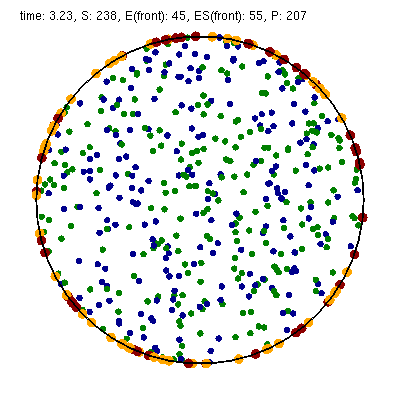
\includegraphics[height=5 cm]{figures/image1}
\caption{Graphical output of template.txt.}
\label{fig:template}
\end{figure}

This file shows enzymatic catalysis, in which green dots are substrate, blue dots are product, enzyme is dark red, and enzyme-substrate complexes are orange. The substrate and product molecules are ``solution phase'', while the enzyme and enzyme-substrate complexes are ``surface-bound'' (e.g. the enzyme is an integral membrane protein).

Note that you can zoom in or out with the ``='' and ``-'' keys and you can pan with shift-arrow keys (arrow keys enable rotating with 3D simulations, but not here because this is a 2D simulation). Pressing ``0'' returns to the default view. You can also press shift-``T'' to take a snapshot of the output, the space bar to pause the simulation, or shift-``Q'' to quit the simulation.

Here is the complete Smoldyn input file for the template.txt simulation. This file includes most of Smoldyn's core features.

\begin{lstlisting}[style=SSAC]
# Smoldyn configuration file template.
# List basic file information here, including your name, the development date,
# what this file does, the model name if you want one, the file version, distribution
# terms, etc. Also, importantly, list the units used in this file, e.g. microns and
# milliseconds. This template file is here to be edited. There is no need to maintain
# any of the current text, or to keep any references to Steve Andrews, or the history
# of this file.

# Enzymatic reactions on a surface, by Steve Andrews, October 2009.
# This model is in the public domain. Units are microns and seconds.
# The model was published in Andrews (2012) Methods for Molecular Biology, 804:519.
# It executes a Michaelis-Menten reaction within and on the surface of a 2D circle.


# Model parameters
define K_FWD 0.001		# substrate-enzyme association reaction rate
define K_BACK 1			# complex dissociation reaction rate
define K_PROD 1			# complex reaction rate to product
#define TEXTOUTPUT		# uncomment this line for text output

# Graphical output
graphics opengl_good		# level of graphics quality (or none)
frame_thickness 0		# turns off display of the system boundaries

# System space and time definitions
dim 2				# 2D system
boundaries x -1 1		# outermost system boundaries on x axis
boundaries y -1 1		# outermost system boundaries on y axis
time_start 0			# simulation starting time
time_stop 10			# simulation stopping time
time_step 0.01			# simulation time step

# Molecular species and their properties
species S E ES P		# species. S=substrate, E=enzyme, ES=complex, P=product
difc S 3			# diffusion coefficients
difc P 3
color S(all) green		# colors for graphical output
color E(all) darkred
color ES(all) orange
color P(all) darkblue
display_size all(all) 0.02	# display sizes for graphical output
display_size E(all) 0.03
display_size ES(all) 0.03

# Surfaces in the system and their properties
start_surface membrane		# start definition of surface
 action all both reflect	# all molecules reflect at both surface faces
  color both black		# surface color for graphical output
  thickness 1			# surface display thickness for graphics
  panel sphere 0 0 1 50		# definition of the surface panel
end_surface

# Compartment definitions
start_compartment inside	# the area within the circle is a compartment
  surface membrane		# a surface that defines the compartmet bounds
  point 0 0			# a point that is within the compartment
end_compartment

# Chemical reactions
reaction fwd E(front) + S(bsoln) -> ES(front) K_FWD	# association reaction
reaction back ES(front) -> E(front) + S(bsoln) K_BACK 	# dissociation reaction
product_placement back pgemmax 0.2			# for reversible reactions
reaction prod ES(front) -> E(front) + P(bsoln) K_PROD	# product formation reaction

# Place molecules for initial condition
compartment_mol 500 S inside	# puts 500 S molecules in the compartment
surface_mol 100 E(front) membrane all all	# puts 100 E molecules on surface

# Output and other run-time commands
text_display time S E(front) ES(front) P	# displays species counts to graphics
ifdefine TEXTOUTPUT				# only run this if needed
  output_files templateout.txt			# file names for text output
  cmd B molcountheader templateout.txt		# text output run at beginning
  cmd N 10 molcount templateout.txt		# text output run every 10 time steps
endif

end_file			# end of this file
\end{lstlisting}

\subsection*{Comments}

All text after a ``\#'' character is a comment and is ignored by Smoldyn.  In these comments, it is good practice to list basic information about the model such as what it represents, the model units, who wrote the file, and distribution terms.  This particular file has comments on almost every line in order to explain what's happening, but this is typically more annoying than useful.

\subsection*{Measurement units}

Notably absent from input file are any measurement units. Instead, you need to choose a single set of units and to then use these throughout the file. For example, cgs units (centimeter-gram-second) and mks units (meter-kilogram-second) are two standard unit systems. These are too large-scale to be convenient for most Smoldyn simulations, so micron-second and nanometer-microsecond tend to be preferable. The following table lists reasonably typical values for different processes in several different unit systems.

\begin{longtable}[c]{llllll}
&& Diffusion & Unimolec. & Bimolecular & Adsorption\\
& Concentration & coefficient & reactions & reactions & rates\\
\hline \\
Typical value & 10 $\mu$M & 10 $\mu$m$^2$s$^{-1}$ & 1 s$^{-1}$ & $10^5$ M1s$^{-1}$ & 1 $\mu$m s$^{-1}$\\
mks & $6\cdot10^{21}$ m$^{-3}$ & $10^{-11}$ m$^2$s$^{-1}$ & 1 s$^{-1}$ & $1.7\cdot10^{-22}$ m$^3$s$^{-1}$ & $10^{-6}$ m s$^{-1}$\\
cgs & $6\cdot10^{15}$ cm$^{-3}$ & $10^{-7}$ cm$^2$s$^{-1}$ & 1 s$^{-1}$ & $1.7\cdot10^{-16}$ cm$^3$s$^{-1}$ & $10^{-4}$ cm s$^{-1}$\\
$\mu$m-ms & 6000 $\mu$m$^{-3}$ & $10^{-2}$ $\mu$m$^2$ms$^{-1}$ & $10^{-3}$ ms$^{-1}$ & $1.7\cdot10^{-7}$ $\mu$m$^3$ms$^{-1}$ & $10^{-3}$ $\mu$m ms$^{-1}$\\
$\mu$m-s & 6000 $\mu$m$^{-3}$ & 10 $\mu$m$^2$s$^{-1}$ & 1 s$^{-1}$ & $1.7\cdot10^{-4}$ $\mu$m$^3$s$^{-1}$ & 1 $\mu$m s$^{-1}$\\
nm-ms & $6\cdot10^{-6}$ nm$^{-3}$ & $10^4$ nm$^2$ms$^{-1}$ & $10^{-3}$ ms$^{-1}$ & 170 nm$^3$ms$^{-1}$ & 1 nm ms$^{-1}$\\
nm-$\mu$s & $6\cdot10^{-6}$ nm$^{-3}$ & 10 nm$^2$$\mu$s$^{-1}$ & $10^{-6}$ $\mu$s$^{-1}$ & 0.17 nm$^3$$\mu$s$^{-1}$ & $10^{-3}$ nm $\mu$s$^{-1}$\\
px-ms & $6\cdot10^{-3}$ px$^{-3}$ & 100 px$^2$ms$^{-1}$ & $10^{-3}$ ms$^{-1}$ & 0.17 px$^3$ms$^{-1}$ & 0.1 px ms$^{-1}$\\
\end{longtable}

A pixel, abbreviated px, is defined as a length of 10 nm. In the concentration column, ``6'' is short for 6.022045. In the bimolecular reactions column, 1.7 is short for 1.660565.

\subsection*{Model parameters}

It is easier to read and edit Smoldyn files if the model parameters that you might want to vary are not hard-coded into the model, but are collected at the top of the file in a collection of define statements. These statements instruct Smoldyn to perform simple text replacement, replacing every subsequent instance of the matching text with the following substitution text. The statement  \ttt{define K\_FWD 0.001}, for example, tells Smoldyn to replace any subsequent  \ttt{K\_FWD} text with  \ttt{0.001}; in this case, this is a reaction rate constant. The substitution text can be a number, multiple numbers, a string, or even nothing at all.

\subsection*{Graphical output}

Graphical output can be displayed with several levels of quality. At the bottom end is no output at all, achieved with the  \ttt{graphics none} statement or by using a  \ttt{-t} flag on the command line (e.g.  \ttt{smoldyn template.txt -t}). Next the  \ttt{graphics opengl} level produces crude graphics,  \ttt{graphics opengl\_good} is passable, and  \ttt{opengl\_better} is reasonably good. Improving the graphics quality slows simulations down, so a good approach is to use the plain  \ttt{opengl} level for model development, no graphics when generating simulation results, and  \ttt{opengl\_better} when preparing publication figures.

As used here, the framethickness statement tells Smoldyn to not show a frame around the entire simulation volume. There are also other statements for controlling the background color, the frame display, etc.

\subsection*{Space and time}

Smoldyn can run simulations in 1, 2, or 3 dimensions. Here, the  \ttt{dim 2} statement says that this is a 2D simulation. The following two  \ttt{boundaries} statements define the system volume, showing that it extends from -1 to 1 on the x axis, and then the same on the y axis. Smoldyn still tracks any molecules beyond these boundaries but it becomes less efficient if there are substantial dynamics there.

Simulations use fixed time steps. They start at the time given with  \ttt{time\_start}, stop at the time given with  \ttt{time\_stop} and have steps with the size given with  \ttt{time\_step}. For typical simulations of subcellular processes, 10 ms is often a reasonable time step. Longer time steps make the simulation run faster and shorter time steps produce more accurate results. Before starting a long series of simulations, it is good practice to run several tests first to ensure that the time step is short enough to produce results of the desired accuracy but also long enough for adequate efficiency.

\subsection*{Molecules}

All of the chemical species in the simulation need to be declared with a  \ttt{species} statement before they can be used in the simulation (except when using rule-based modeling, as explained later on).

The following  \ttt{difc},  \ttt{color}, and  \ttt{display\_size} statements define the diffusion coefficients, graphical display colors, and graphical display sizes for these different species. These parameters can vary for different molecule states, meaning whether the molecule is in solution or bound to a surface; the latter case, it can be bound to a surface in any of the ``front'', ``back'', ``up'', or ``down'' states. If no molecule state is listed, such as in the statement  \ttt{difc S 3}, this applies to only the solution state; if one of these substrate molecules were to bind to a surface, it would not diffuse because the surface-bound diffusion coefficients are all still equal to 0. For convenience, these species parameters can be defined for all of the states at once by using ``all'' as the state, such as in the statement  \ttt{color S(all) green}.

The behavior of the \ttt{display\_size} statement depends on the graphical output style. For the ``opengl'' graphics level, the display size value is in pixels. Here, numbers from 2 to 4 are typically good choices. For the two better graphics options, the display size value is the radius with which the molecule is drawn, using the same units as elsewhere in the input file.

\subsection*{Surfaces}

Smoldyn surfaces are infinitesimally thin structures that can be used to represent cell membranes, obstructions, system boundaries, or other things. They are 2D structures in 3D simulations, or 1D lines or curves in 2D simulations (or 0D points in 1D simulations). Each surface has a ``front'' and a ``back'' face, so molecules can interact differently with the two sides of a surface. Each surface is composed of one or more ``panels'', where each panels can be a rectangle, triangle, sphere, hemisphere, cylinder, or a disk. Surfaces can be disjoint, with separate non-connected portions. However, all portions of a given surface type are displayed in the same way and interact with molecules in the same way.

Surfaces get defined in ``surface blocks,'' which start with  \ttt{start\_surface} and the surface name, and end with  \ttt{end\_surface}. Within the surface block, define molecule interactions with this surface using the  \ttt{action} or  \ttt{rate} statements. In this case, the statement  \ttt{action all both reflect} states that molecules of all species should reflect off of this surface upon collision with either of the two faces. Other action options are  \ttt{absorb} and  \ttt{transmit}, for absorption by the surface, and transmission through the surface, respectively. Use the  \ttt{rate} statement, which is not used in this file, for adsorption, desorption, or partial transmission through a surface.

Define surface graphics using the color and thickness statements. For 3D simulations, the  \ttt{polygon} statement is useful as well. With it, you can specify whether you want Smoldyn to draw just the panel edges (typically the best choice), the entire panel face, or other options.

Surface panels definitions list each panel within the surface, including details about the panel location, orientation, and display. The sequence of these parameters is hard to remember but is described in the reference section of this manual. In this particular case, the statement  \ttt{panel sphere 0 0 1 50} indicates that there should be a single spherical panel (actually a circle because this is a 2D simulation) with its center at the coordinates (0,0). This circle should have radius of 1 and get drawn with 50 straight line segments. The front face of this circle is on the outside and the back face is on the inside (this can be reversed by giving the radius with a negative value).

\subsection*{Compartments}

Compartments are defined regions of space. They have essentially no role in the actual functioning of the simulation but can be useful for placing and observing molecules. Their only simulation role is that reactions can be qualified so that they only occur within specific compartments (which does not happen in this input file).

As with surfaces, compartments are defined with blocks of text. Each block starts with  \ttt{start\_compartment} and the compartment name and ends with  \ttt{end\_compartment}. Within the block, list the surface or surfaces that form the boundaries to this compartment. Also, list at least one ``interior-defining point'' (a set of coordinates) that is inside the compartment, so Smoldyn knows which region is the inside and which is the outside. In this file, the circle is the compartment bounding surface and a point at the center of the circle is the interior-defining point, so the compartment represents the entire region within the circle.

Intuitively, the region of a compartment should be defined as everywhere in space to which one can ``walk'' from the interior-defining point, without crossing any of the bounding surfaces. However, for computational efficiency, Smoldyn uses a slightly different definition. In Smoldyn, the region of a compartment is everywhere in space from which one can ``see'' the interior-defining point using a straight line, without crossing any of the bounding surfaces. The difference between the definitions is minimal is many cases, but can be important.

\subsection*{Reactions}

Smoldyn only simulates elementary chemical reactions, such as unimolecular conversions and bimolecular associations. Multistep reactions, like Michaelis-Menten reactions, need to be constructed from their elementary reactions. List each reaction with the  \ttt{reaction} statement followed by: the reaction name, the reactants, a forward arrow, the products, and the reaction rate constant.

Both reactant and product names can be followed by their states, listed in parentheses. These states are essentially the same as those for the molecule diffusion coefficient and color statements. The difference is that the solution state now subdivides into the two pseudo-states ``fsoln'' and ``bsoln'', where these indicate the solution state that is on the front or back, respectively, of the relevant surface. In this file, for example, the reaction  \ttt{reaction fwd E(front) + S(bsoln) -> ES(front) K\_FWD} occurs between enzyme molecules that are surface-bound in their front state and substrate molecules that are in the solution on the back side of the surface, meaning inside the circle. The product is in the front state. If any state is not listed, Smoldyn assumes the ``fsoln'' state (which is identical to the normal solution state).

To simulate unimolecular reactions, Smoldyn computes a reaction probability per time step. Then, during the simulation, it reacts molecules of the given species with the computed probability at each time step. For bimolecular reactions, Smoldyn combines the reaction rate constant, the reactant diffusion coefficients, and the simulation time step to compute a ``binding radius''. Larger reaction rate constants lead to larger binding radii. During the simulation, if two reactants end up within this binding radius of each other at the end of a time step, then Smoldyn performs the reaction. It is also possible to specify that these reactions should only happen with some probability, but this has very little benefit and so is not standard.

Reversible association/dissociation reactions have the additional complexity that the dissociation product molecules start out in close proximity and so have a high probability of rapidly reacting with each other in a so-called ``geminate recombination''. Smoldyn controls the probability of geminate recombinations, as opposed to products diffusing apart and not re-reacting, by initially separating products by an ``unbinding radius''. There is extremely little information in the scientific literature about what the probability of geminate recombinations should be. As a result, Smoldyn sets this probability to a maximum value of 0.2 by default. I chose this to balance the physical situation that product molecules should be produced reasonably close together with the simulation practicality that simulating geminate recombinations is computationally costly. Because this default value is a very rough guess, Smoldyn emits a warning if it is not over-ridden by the input file. The line  \ttt{product\_placement back pgemmax 0.2} prevents this warning by explicitly specifying that the products of the reaction named back should be placed so that the maximum probability of geminate recombination is 0.2.

Similar reaction statements can be used for other molecule-molecule interactions, such as excluded volume interactions and ``conformational spread reactions''; in the latter case, the proximity of one molecule affects the unimolecular reactions of another molecule.

\subsection*{Initial molecule placement}

Place molecules in a simulation at the starting time using several  \ttt{mol} statements. The plain  \ttt{mol} statement place molecules with random or specific positions in the simulation volume, the  \ttt{compartment\_mol} statement places molecules randomly in a given compartment, and the  \ttt{surface\_mol} statement places molecules with random or specific positions on a given surface. In the last case, the molecule state needs to be specified. In the example file, the statement  \ttt{surface\_mol 100 E(front) membrane all all} instructs Smoldyn to place 100 enzyme molecules onto the membrane surface in their front state, and that these molecules should be placed randomly on all panel shapes and all panels of those shapes (which, in this case, was only one panel).

\subsection*{Output and Commands}

Smoldyn supports a few general output statements. One of those is  \ttt{text\_display}, which can display the time and molecule counts to the graphical output window. Other output statements can save TIFF files of the graphical output for recording snapshots of the simulation or complete movies.

Commands are also useful for output, and for many other things. These run-time commands can be thought of as a virtual experimenter who has permission to manipulate or observe the simulated system in a wide variety of ways. Whereas the rest of the simulation is supposed to be physically accurate, there are no such restrictions for commands.

If commands are used to output text to files, then Smoldyn needs to know what those files are beforehand, which is the purpose of the  \ttt{output\_files} statement. If those files already exist, then Smoldyn checks with the user first before overwriting them. To suppress this warning, run Smoldyn with a  \ttt{-w} option on the command line (e.g.  \ttt{smoldyn template.txt -w}).

Each command is entered with the same general format. They start with  \ttt{cmd}, list the times when the command should be executed, give the name of the specific command, and then give the parameters of that command. For example,  \ttt{cmd B molcountheader templateout.txt} indicates that the command should be run before the simulation starts, the command is  \ttt{molcountheader} (which writes out a list of the species names), and the command should send its output to the file templateout.txt. Similarly,  \ttt{cmd N 10 molcount templateout.txt} indicates that the command should be run every 10 time steps, the command is molcount (which counts the molecules of each species), and the command should also send its output to templateout.txt.

Smoldyn supports quite a lot of commands, all of which are listed in the second half of the reference section, at the back of this manual.

In this particular example file, note the use of the  \ttt{ifdefine TEXTOUTPUT} statement. This is used to easily turn on or turn off text output by commenting the  \ttt{define TEXTOUTPUT} statement at the top of the file.

\section{Conclusions}

This chapter has presented most of what you know to read and write Smoldyn input files. If you have not done so already, I recommend stopping here and experimenting with Smoldyn. At a minimum, it is helpful to edit and run some of the example files. Ideally, this is a good time to copy an example file into your own directory and then completely rewrite it to create your own model. As you go along, refer to the reference section for the details of how specific statements and commands work. Also, read other chapters in this manual as questions arise.

If you start using Smoldyn for actual research, then it is important that you understand what the software is actually doing. It is also helpful to learn about Smoldyn's more advanced features, how to automate simulations, and what makes simulations fast or slow. The rest of this manual addresses these topics.

% Part II: Smoldyn Components
\addcontentsline{toc}{chapter}{Part II: Smoldyn Components}

% The Configuration File
\chapter{The Configuration File}

This is the first of the chapters that focuses on a specific aspect of Smoldyn, in this case the configuration or input file. These chapters are arranged with more elementary material first and more advanced material afterwards.

\section{Runtime flags}

When starting Smoldyn from the command line, you can follow the filename with runtime flags, of which the options are listed below. Any combination of flags may be used, and in any order.

\begin{longtable}[c]{lll}
Command & Smoldyn\\
line & query & Result\\
\hline\\
 & - & normal: parameters displayed and simulation run\\
\ttt{-o} & o & suppress output: text output files are not opened\\
\ttt{-p} & p & parameters only: simulation is not run\\
\ttt{-q} & q & quiet: parameters are not displayed\\
\ttt{-t} & t & text only: no graphics are displayed\\
\ttt{-V} & V & display version number and quit\\
\ttt{-v} & v & verbose: extra parameter information is displayed\\
\ttt{-w} & w & suppress warnings: no warnings are shown\\
\ttt{--define }\param{x=y} &  & set a text macro definition\\
\end{longtable}

\section{Configuration file syntax}

Configuration files, such as bounce3.txt, are simple text files. The format is a series of text lines, each of which needs to be less than 256 characters long. On each line of input, the first word describes which parameters are being set, while the rest of the line lists those parameters, separated by spaces. If Smoldyn encounters a problem with a line, it displays an error message and terminates. Possible problems include missing parameters, illegal parameter values, too many parameters, unrecognized molecule, surface, or reaction names, unrecognized statements, or others.

In most cases, statements may be entered in any order, although some are required to be listed after others. The required sequence is not always obvious, so it is usually easiest to just try what seems most reasonable and then fix any errors that Smoldyn reports. Also, a few instructions can only be entered once, whereas others can be entered multiple times. If a parameter is entered more than once, the latter value overwrites the prior one. Parameters that are not defined in the configuration file are assigned default values.

\section{Variables and formulas}

Smoldyn supports numeric variables. Set them using the variable statement, such as \ttt{variable x = 100} (spaces are required here). Also, essentially all numeric inputs can be entered with a formula. For example, if you want a reaction rate to be two times the value of \ttt{x}, enter it as \ttt{2*x} (spaces are not allowed within formulas). Smoldyn's formula processing supports arithmetic (+,-,*,/), modulo division (\%), powers (\^{}), and all levels of parentheses. It also supports many standard functions, such as exp, sin, sqrt, etc.

\section{Statements about the configuration file}

A few statements control the reading of the configuration file, which are now described in more detail. The first, shown in the first line of bounce3.txt, is a comment. A \# symbol indicates that the remainder of the line should be ignored, whether it is the whole line as it is in bounce3.txt or just the end of the line. It is also possible to comment out entire blocks of the configuration file using \ttt{/*} to start a block-comment and \ttt{*/} to end it. For these, the \ttt{/*} or \ttt{*/} symbol combinations are each required to be at the beginning of configuration file lines. The remainder of those lines is ignored, along with any lines between them.

It is possible to separate configuration files into multiple text files. This is done with the statement \ttt{read\_file}, which simply instructs Smoldyn to continue reading from some other file until that one ends with \ttt{end\_file}, which is followed by more reading of the original file. The \ttt{read\_file} statement may be used anywhere in the configuration file, including within reaction definition and surface definition blocks (described below) and within files that were themselves called with a \ttt{read\_file} statement. The configuration file examples/S2\_config/config.txt illustrates these statements.

\section{Text substitution macros}

You can use \ttt{define} statements to instruct Smoldyn to perform simple text substitution as it reads in a configuration file. As a typical example, you might define your reaction rate constants at the top of a configuration file using define statements (e.g. \ttt{define k1 100}) and then use the key later on in the file rather than the actual number. This leads to a file that is more readable and easier to modify. One definition is set automatically: \ttt{FILEROOT} is replaced by the current file name, without path information and without any text that follows a ``.''. Prior definitions are overwritten with new ones without causing errors or warnings. These definitions have local scope, meaning that they only lead to text replacement within the current configuration file, and not to those that it reads with \ttt{read\_file}. To create a definition with broader scope, use \ttt{define\_global}; the scope of these definitions is throughout the current configuration file, as well as any file or sub-file that is called by the current file. A configuration file that calls the current one is not affected by a \ttt{define\_global}. To remove a definition, or all definitions, use \ttt{undefine}.

\ttt{define} statements can also be used for conditional configuration file reading. In this case, a definition is made as usual, although there is no need to specify any substitution text. Later in the file, the \ttt{ifdefine}, \ttt{else}, and \ttt{endif} statements lead to reading of different portions of file, depending on whether the definition was made or not. A variant of the ifdefine statement is the \ttt{ifundefine} statement. These conditional statements should work as expected if they are used in a normal sort of manner (see any programming book for basic conditional syntax), which includes support for nested \ttt{if} statements. They can also be used successfully with highly abnormal syntaxes (for example, an \ttt{else} toggles reading on or off, regardless of the presence of any preceding \ttt{ifdefine} or \ttt{ifundefine}), although this use is discouraged since it will lead to confusing configuration files, as well as files that may not be compatible with future Smoldyn releases.

Text substitution can also be directed from the command line. If you include the command line option \ttt{--define}, followed by text of the form \param{key = replacement} (do not include spaces, although if you want spaces within the replacement text, then enclose it in double quotes), this is equivalent to declaring text substitution using the define\_global statement within a configuration file. For example, to the file cmdlinedefine.txt includes the macro key \ttt{RDIFC} but does not define it. To run this file, define the macro key on the command line like

$$\ttt{smoldyn examples/S2\_config/cmdlinedefine.txt --define RDIFC=5}$$

This feature simplifies running multiple simulations through a shell script. Essentially any number of definitions can be made this way. If the same key text is defined both on the command line and in the configuration file, the former takes priority.

\section{Running multiple simulations using scripts}

It is often useful to simulations over and over again, whether to collect statistics, to look for rare events, or to scan over parameter ranges. This is easily accomplished by writing a short Python script, or a script in some other high level language such as R, MatLab, Mathematica, etc. The following Python script is at S2\_config/pyscript.py. It runs the file paramscan.txt several times using different parameter values, with results sent to the standard output and also saved to different files.

\begin{lstlisting}[style=SSAPython]
# A python script for scanning a parameter
import os

simnum=0
for rxnrate in [0.01,0.02,0.05,0.1,0.2,0.5,1]:
	simnum+=1
	string='smoldyn paramscan.txt --define RXNRATE=%f --define SIMNUM=%i -tqw' %(rxnrate,simnum)
	print(string)
	os.system(string)
\end{lstlisting}
Run this script by entering \ttt{python pyscript.txt}.

Another method for running batches of simulations is for your script to generate a Smoldyn-readable text file with the appropriate parameters, say with the file name myparams.txt. Then, in your master Smoldyn file, which might also be called from the same script, include the line \ttt{read\_file myparams.txt}, which reads in the necessary parameters.

\section{Summary}

The following table summarizes the statements that deal with the configuration file.

\begin{longtable}[c]{ll}
Statement & meaning\\
\hline\\
\ttt{\#} & single-line comment\\
\ttt{/*} � \ttt{*/} & multi-line comment\\
\ttt{read\_file} \param{filename} & read filename, and then return\\
\ttt{end\_file} & end of this file\\
\ttt{define} \param{key substitution} & local macro replacement text\\
\ttt{define\_global} \param{key substitution} & global macro replacement text\\
\ttt{undefine} \param{key} & undefine a macro substitution\\
\ttt{ifdefine} \param{key} & start of conditional reading\\
\ttt{ifundefine} \param{key} & start of conditional reading\\
\ttt{else} & else condition for conditional reading\\
\ttt{endif} & ends conditional reading\\
\end{longtable}



% Space and time
\chapter{Space and time}

\section{Space}

Smoldyn simulations can be run in a system that is 1, 2, or 3-dimensional. These can be useful for accurate simulations of systems that naturally have these dimensions. For example, a 2-dimensional system can be useful for investigating diffusional dynamics and interactions of transmembrane proteins. Smoldyn does not permit 4 or more dimensional systems because it is not clear that they would be useful. Define the system dimensionality with the dim statement, which needs to be one of the first statements in a configuration file.

Along with the system dimensionality, it is necessary to specify the outermost boundaries of the system. In most cases, it is best to design the simulation so that all molecules stay within the system boundaries, although this is not required. All simulation processes are performed outside of the system boundaries exactly as they are within the boundaries. Boundaries are used by Smoldyn to allow efficient simulation and for scaling the graphical display. They are typically defined with the boundaries statement, as seen in the example S1\_intro/bounce3.txt. Boundaries may be reflective, transparent, absorbing, or periodic. Reflective means that all molecules that diffuse into a boundary will be reflected back into the system. Transparent, which is the default type, means that molecules just diffuse through the boundary as though it weren't there. With absorbing boundaries, any molecule that touches a boundary is immediately removed from the system. Finally, with periodic boundaries, which are also called wrap-around or toroidal boundaries, any molecule that diffuses off of one side of space is instantly moved to the opposite edge of space; these are useful for simulating a small portion of a large system while avoiding edge effects.

On rare occasion, it might be desirable to have asymmetric system boundary types. For example, one side of a system might be reflective while the other is absorbing. To accomplish this, use the \ttt{low\_wall} and \ttt{high\_wall} statements instead of a \ttt{boundary} statement. This is illustrated in the example file S3\_space/bounds1.txt.

These boundaries of the entire system are different from surfaces, which are described below. However, they have enough in common that Smoldyn does not work well with both at once. Thus, \textit{if any surfaces are used, the system boundaries will always behave as though the types are transparent, whether they are defined that way or not}. Thus, if there are surfaces, it is usually best to use the boundaries statement without a type parameter, which will lead to the default transparent type. To account for the transparent boundaries, an outside surface may be needed that keeps molecules within the system. The one exception to these suggestions arises for systems with both surfaces and periodic boundary conditions. To accomplish this with the maximum accuracy, set the boundary types to periodic (although they will behave as though they are transparent) and create jump type surfaces, described below, at each outside edge that send molecules to the far sides. The reason for specifying that the boundaries are periodic is that they will then allow bimolecular reactions that occur with one molecule on each side of the system. This will probably yield a negligible improvement in results, but nevertheless removes a potential artifact. This is illustrated in the example S3\_space/bounds2.txt.

\section{Time}

A simulation runs for a fixed amount of simulated time, using constant length time steps. The simulation starting time is set with \ttt{time\_start} and the stopping time is set with \ttt{time\_stop}. For simulations that are interrupted and then continued, the \ttt{time\_now} statement allows the initial time to be set to a value that is intermediate between the starting and stopping times.

The size of the time step is set easily enough with \ttt{time\_step}, although knowing what value to use is an art. Smoldyn always becomes more accurate, and runs more slowly, as shorter time steps are used. Thus, an important rule for picking a time step size is to compare the results that are produced for one value with those produced with a time step that is half as long; if the results are identical, within stochastic noise, then the longer time step value is adequate. If not, then a smaller time step needs to be used.

As an initial guess for what time step to use, time steps can be chosen from the spatial resolution that is required. The average displacement of a molecule, which has diffusion coefficient $D$, during one time step is $s = \sqrt{2D \Delta t}$, where $\Delta t$ is the time step. Turning this around, to achieve spatial resolution of $s$, the time step needs to obey
$$\Delta t < \frac{s^2}{2D_{max}}$$ 
where $D_{max}$ is the diffusion coefficient of the fastest diffusing species. The overall spatial resolution for a simulation, which is the largest rms step length, is displayed in the ``molecule parameters'' section of the configuration file diagnostics output. For good accuracy, the spatial resolution should be significantly smaller than geometric features or than radii of curvature, for curved objects.

Other considerations for choosing the time step are the characteristic time scales of the unimolecular and bimolecular reactions. For good accuracy, the time step should generally be significantly shorter than the characteristic time scale of any reaction. Using $k$ as the reaction rate constants, unimolecular and bimolecular reactions lead to the respective time step constraints
$$\Delta t < \frac{1}{k}$$
$$\Delta t < \frac{[\textrm{A}]+[\textrm{B}]}{k[\textrm{A}][\textrm{B}]}$$
The latter equation is for the reaction A + B $\rightarrow$ products. These values are displayed in the ``reaction parameters'' section of the configuration file diagnostics output. While the time scale for unimolecular reactions is independent of concentrations, the time scale for bimolecular reactions clearly depends on concentrations. Thus, the time scale that is displayed for bimolecular reactions is only a rough guide at best; it does not account for the changing concentrations of the reactants nor for local variations in concentrations.
As an initial guess, the time step that is chosen should be the smallest of those that are suggested here for all of these processes. Afterwards, it is usually worth running several trial simulations with longer or shorter time steps to see what the longest time step is that still yields sufficiently accurate results.

\section{Summary of statements that define space and time}

The following table summarizes the statements for defining space and time.

\begin{longtable}[c]{ll}
Statement & function\\
\hline\\
\ttt{dim} \param{dim} & system dimensionality: 1, 2, or 3\\
\ttt{boundaries} \param{dim pos1 pos2} & system boundaries on dimension \param{dim}\\
\ttt{boundaries} \param{dim pos1 pos2} type & same, for systems without surfaces\\
\ttt{low\_wall} \param{dim pos type} & specify single low-side boundary\\
\ttt{high\_wall} \param{dim pos type} & specify single high-side boundary\\
\ttt{time\_start} \param{time} & starting time of simulation\\
\ttt{time\_stop} \param{time} & stopping time of simulation\\
\ttt{time\_step} \param{time} & time step for the simulation\\
\ttt{time\_now} \param{time} & current time of the simulation
\end{longtable}

\section{Technical discussion of time steps}

A major focus of the design of Smoldyn has been to make it so that results are indistinguishable from those that would be obtained if the simulated time increased continuously. This goal cannot be achieved perfectly. Instead, the algorithms are written so that the simulation approaches the Smoluchowski description of reaction-diffusion systems as the time step is reduced towards zero. Also, it maintains as much accuracy as possible for longer time steps. This topic is discussed in detail in the research paper ``Stochastic simulation of chemical reactions with spatial resolution and single molecule detail'' by Steven Andrews and Dennis Bray (Physical Biology 1:137-151, 2004).

In concept, the system is observed at a fixed time, then it evolves to some new state, then it is observed again, and so forth. This leads to the following sequence of program operations:

\begin{longtable}[c]{l}
--------------- time = $t$ ---------------\\
observe and manipulate system\\
graphics are drawn\\
molecules diffuse\\
desorption and surface-state transitions\\
surface or boundary interactions\\
0th order reactions\\
1st order reactions\\
2nd order reactions\\
reaction products are added to system\\
surface interactions of reaction products\\
------------- time = $t + \Delta t$ -------------
\end{longtable}

After commands are run, graphics are displayed to OpenGL if that is enabled. The evolution over a finite time step starts by diffusing all mobile molecules. In the process, some end up across internal surfaces or the external boundary. These are reflected, transmitted, absorbed, or transported as needed. Next, reactions are treated in a semi-synchronous fashion. They are asynchronous in that all zeroth order reactions are simulated first, then unimolecular reactions, and finally bimolecular reactions. With bimolecular reactions, if a molecule is within the binding radii of two different other molecules, then it ends up reacting with only the first one that is checked, which is arbitrary (but not necessarily random). Reactions are synchronous in that reactants are removed from the system as soon as they react and products are not added into the system until all reactions have been completed. This prevents reactants from reacting twice during a time step and it prevents products from one reaction from reacting again during the same time step. As it is possible for reactions to produce molecules that are across internal surfaces or outside the system walls, those products are then reflected back into the system. At this point, the system has fully evolved by one time step. All molecules are inside the system walls and essentially no pairs of molecules are within their binding radii (the exception is that products of a bimolecular reaction with an unbinding radius might be initially placed within the binding radius of another reactant).

Each of the individual routines that is executed during a time step exactly produces the results of the Smoluchowski description, or yields kinetics that exactly match those that were requested by the user. However, the simulation is not exact for all length time steps because it cannot exactly account for interactions between the various phenomena. For example, if a system was simulated that only had unimolecular reactions and the products of those reactions did not react, then the simulation would yield exactly correct results using any length time step. However, if the products could react, then there would be interactions between reactions and there would be small errors. In this case, the error arises because Smoldyn does not allow a molecule to be in existence for less than the length of one time step.

% Molecules
\chapter{Molecules}

\section{About molecules}

In Smoldyn, each individual molecule is represented as a separate point-like particle. These particles have no volume, so they do not collide with each other when they are simply diffusing (however, see ``excluded volume reactions'' in the reactions section, below, which can give molecules excluded volume). Because of the rapid collisions that occur for solvated molecules, both rotational correlations and momentum correlations damp out rapidly in most biochemical systems, so orientations and momenta are ignored in Smoldyn as well.

Each molecule has a molecular species. Enter the names for these species with the species statement. You can refer to these species by the same names afterwards, or you can refer to multiple species at a time using either wildcard symbols or by defining species groups.

Each molecule is allowed to exist in any of five states: (1) not bound to any surface (called solution state), (2) bound to the front of a surface, (3) bound to the back of a surface, (4) bound across a surface in the ``up'' direction, or (5) bound across a surface in the ``down'' direction. While the surface-bound states are intended to represent specific molecule attachments to membranes, they can also be used for other purposes; for example, you can specify that a trans-membrane protein is normally in its ``up'' state, but that it's in its ``down'' state when it is in a lipid raft.

Molecules that are not bound to surfaces are added with the mol statement. This is a reasonably versatile statement in that, on each axis, it allows molecules to be placed randomly within the simulation volume, randomly within some smaller region, or at a specific location. The \ttt{surface\_mol} statement is used to add molecules that are bound to surfaces, although it cannot be entered in the configuration file until the appropriate surface has been set up. Similarly, \ttt{compart\_mol} is used to add molecules to compartments, which are regions between surfaces, but it also cannot be entered until more things have been set up. The statements about molecules mentioned thus far, with the exception of the last two, are shown in either S1\_intro/bounce3.txt or S4\_molecules/molecule.txt.

\section{Diffusion}

Molecules in Smoldyn diffuse according to the diffusion coefficient that is entered for the appropriate species and state. These coefficients are entered with the \ttt{difc} statement. Although it has not proven to be particularly useful, it is also possible for Smoldyn to simulate anisotropic diffusion, meaning that molecules diffuse more rapidly in some directions than in others. Anisotropic diffusion is specified with a diffusion coefficient matrix using the \ttt{difm} statement.

Isotropic diffusion rates were tested quantitatively with the diffi.txt configuration file. In this file, all molecules start in the center of space, the boundaries are made transparent so molecules diffuse completely freely, and red, green, and blue molecules diffuse with different diffusion coefficients. Using a runtime command in the configuration file, described below, Smoldyn outputs the moments of the molecular distributions to text files. They were analyzed with the Excel file diffi.xls, which is also in the S4\_molecules folder. From this Excel file, the graphical and numerical results are shown below, along with theoretical predictions.

\begin{figure}[h]
\centering
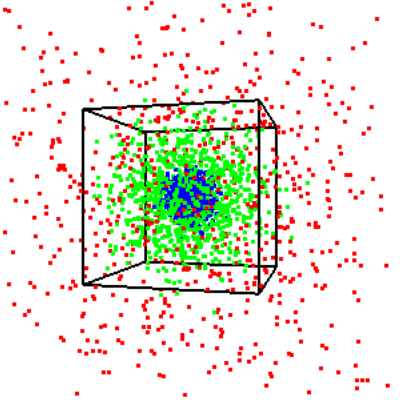
\includegraphics[height=5 cm]{figures/image5}
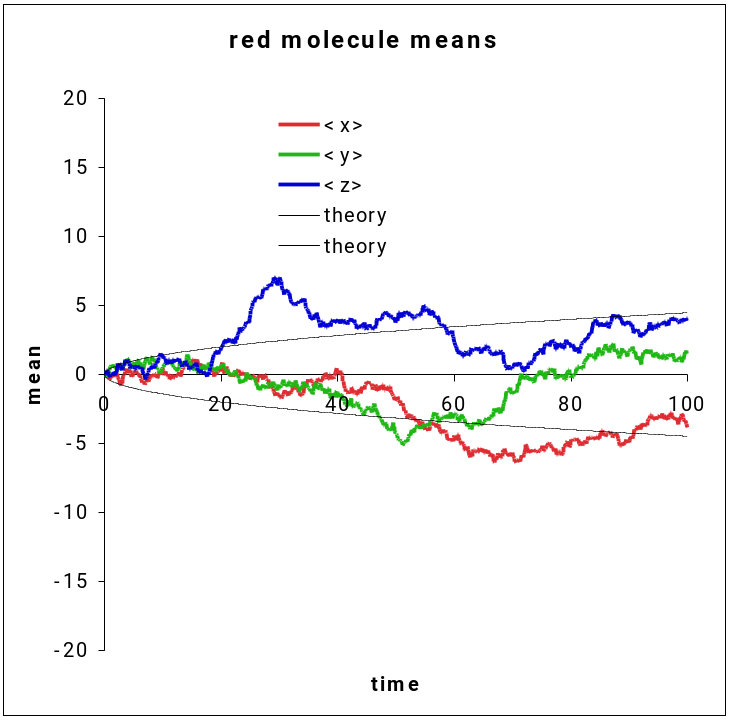
\includegraphics[height=5 cm]{figures/image6}
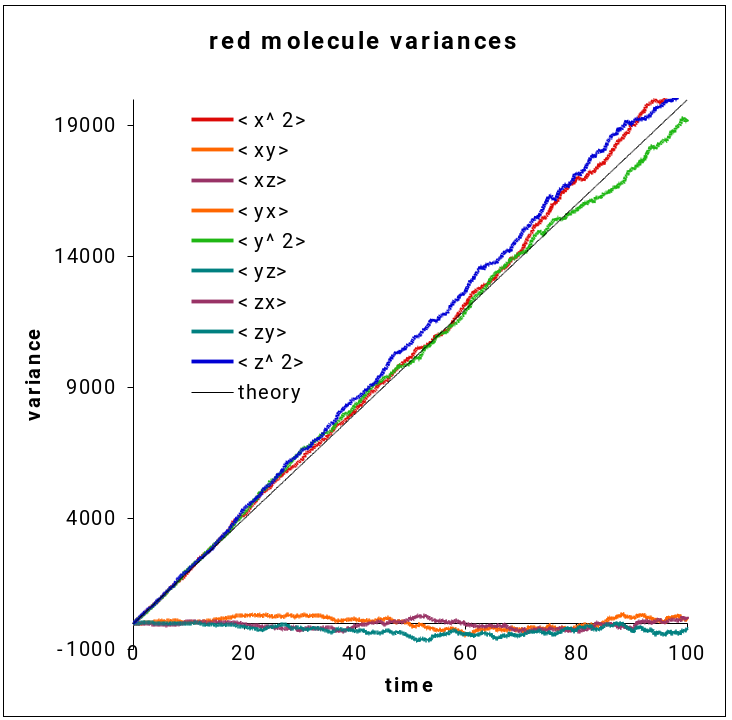
\includegraphics[height=5 cm]{figures/image7}
\caption{Output from file diffi.txt showing quantiatively accurate isotropic diffusion.}
\label{fig:diffi}
\end{figure}

The middle panel of the figure shows that the mean position of the red molecules, on each of the three coordinates, stays near zero although with fluctuations. This is as expected for free diffusion. The expected fluctuation size, shown in the panel with light black lines, is given with
$$|\textrm{mean}-\textrm{starting point}| \approx \sqrt{\frac{2Dt}{n}}$$
where $D$ is the diffusion coefficient, $t$ is the simulation time, and $n$ is the number of molecules. This equation agrees well with simulation data. The second moment of the molecule displacements is a matrix quantity which gives the variance on each pair of axes of the distribution of positions, shown in the third panel. For example, the variance matrix element for axes $x$ and $y$ is
$$v_{xy} = \frac{1}{n} \sum_{i=1}^{n} (x_i - \bar{x})(y_i - \bar{y})$$
The overbars indicate mean values for the distribution. Because diffusion on different axes is independent, the off-diagonal variances ($v_{xy}$, $v_{xz}$, and $v_{yz}$) are expected to be about 0, but with some fluctuations, as is seen in the figure. The diagonal variances ($v_{xx}$, $v_{yy}$, and $v_{zz}$) are each expected to increase as approximately
$$v_{xx} \approx v_{yy} \approx v_{zz} \approx 2Dt$$
Again, this is seen in the figure. Similar figures for the green and blue molecules, which are not presented, showed similarly good agreement between the simulation data and theory.

Anisotropic diffusion was investigated with the example file diffa.txt. In this case, the diffusion equation is
$$\dot{u} = \nabla \cdot \mathbf{D} \nabla u$$
Here, $u$ can be interpreted as either the probability density for a single molecule or as the concentration of a macroscopic collection of molecules, and $\mathbf{D}$ is the diffusion matrix. $\mathbf{D}$ is symmetric. The matrix that is entered in the configuration file for anisotropic diffusion, using the \ttt{difm} statement, is the square root of the diffusion matrix because the square root is much more convenient for calculating expectation molecule displacements. Matrix square roots can be calculated with MatLab, Mathematica, or other methods. Note that the symmetric property of $\mathbf{D}$ implies some symmetry properties for its square root as well (for example, a symmetric square root leads to a symmetric $\mathbf{D}$). If $\mathbf{D}$ is diagonal, the square root of the matrix is found by simply replacing each element with its square root. If $\mathbf{D}$ is equal to the identity matrix times a constant, $D$, the equation reduces to the standard isotropic diffusion equation. The example file diffa.txt illustrates the use of the \ttt{difm} statement; the relevant lines are
\begin{lstlisting}[style=SSAC]
difm red 1 0 0 0 0 0 0 0 2
difm green 1 2 3 2 0 4 3 4 1
\end{lstlisting}
The former line leads to anisotropic diffusion of red molecules with a diffusion coefficient of 1 on the $x$-axis, 0 on the $y$-axis, and 4 on the $z$-axis. The latter leads to anisotropic diffusion with off-diagonal components. This matrix is interpreted to be
$$\sqrt{\mathbf{D}} = \left[ \begin{array}{ccc} 1 & 2 & 3\\ 2 & 0 & 4\\ 3 & 4 & 1 \end{array} \right]$$
Results are shown below

\begin{figure}[h]
\centering
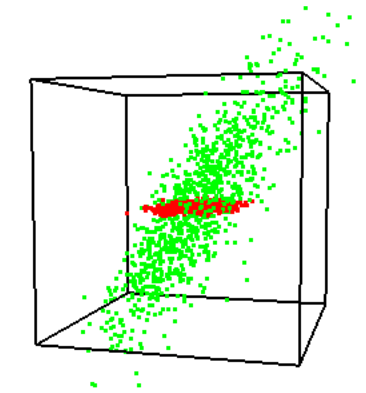
\includegraphics[height=5 cm]{figures/image13}
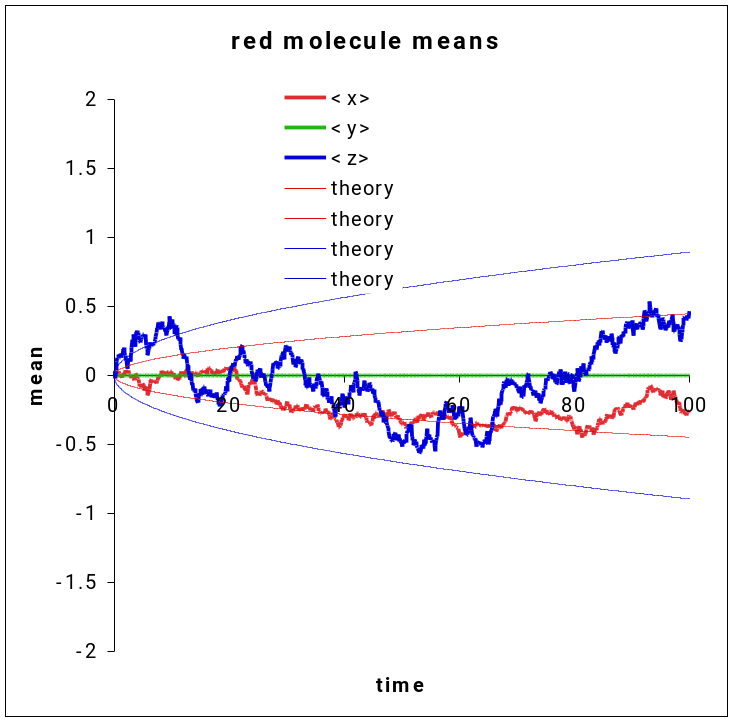
\includegraphics[height=5 cm]{figures/image14}
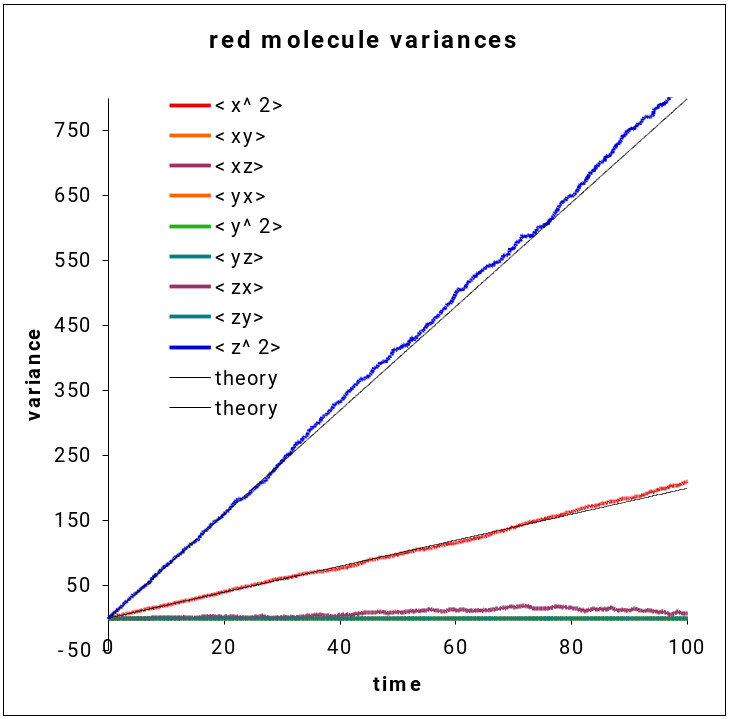
\includegraphics[height=5 cm]{figures/image15}
\caption{Output from diffa.txt showing quantitatively accurate anisotropic diffusion.}
\label{fig:diffa}
\end{figure}

In the figure, it can be seen that the red molecules diffuse only on the $x$-$z$-plane, whereas the green molecules diffuse into an elliptical pattern that is not aligned with the axes. The red molecule data are graphed, where it is shown that $x$-values diffuse slowly, $y$-values don't diffuse at all, and $z$-values diffuse rapidly. The means and variances agree well with theory.

\section{Drift}

In addition to diffusion, molecules can drift, meaning that they move with a fixed speed and in a fixed direction. Up to version 2.26, drift could only be defined relative to the global system coordinates. For this method, which is supported in subsequent versions as well, enter the drift rate using the \ttt{drift} statement, followed by the velocity vector. Surface-bound molecules drift as well, although they are constrained to surfaces, so their actual velocity depends on the overlap of the drift vector and the surface orientation (e.g. a molecule's velocity is zero if the local surface is perpendicular to the drift vector and it equals the drift vector if that vector can lie within the the local surface orientation).

New in version 2.27, surface-bound molecules can also drift relative to the coordinates of their surface panel. Specify this with the \ttt{surface\_drift} statement. For a 2-D system, surfaces are 1-D objects, so the surface-bound drift vector is a single number. It is the drift rate along ``rectangles,'' ``triangles,'' ``spheres,'' etc., all of which are really just different shape lines. For a 3-D system, surfaces are 2-D objects, so the surface-bound drift vector includes two values, which generally use the most obvious orthogonal coordinates for each panel shape. For a cylinder, for example, the former number is the drift rate parallel to the cylinder axis and the latter is the drift rate around the cylinder. A possible use of surface-bound drift would be to simulate molecular motor motion along a cylinder that represents a microtubule.

\section{Molecule lists}

From a user's point of view, Smoldyn molecules follow a Western life trajectory: some chemical reaction causes a new molecule to be born from nothing, it diffuses around in space for a while, and then it undergoes a reaction and vanishes again into nothingness (or maybe goes to molecule heaven). Internally though, the situation is closer to a Wheel of Life: there are a fixed number of molecules that cycle indefinitely between ``live'' and ``dead'' states and which are assigned a new species type at each reincarnation. The dead molecule list is of no importance to the functioning of the simulation, but merely stores molecules when they are not currently active in the simulated system. The size and current population of the dead list are displayed in the molecule section of the configuration file diagnostics if you choose verbose output.

Active molecules in a simulation are stored in one or more live lists. As a default, all live molecules that diffuse, meaning that the diffusion coefficient is non-zero, are stored in a list called ``diffuselist'' while all fixed molecules are stored in a separate live list called ``fixedlist.'' The separation of the molecules into these two lists speeds up the simulation because all molecules in fixedlist can be safely ignored during diffusion calculations or surface checking.

Additional live lists can be beneficial as well. For example, consider the equilibrium chemical reaction A + B $\leftrightarrow$ C. The only bimolecular reaction possible is between A and B molecules, so there is no need to check each and every A-A, B-B, A-C, B-C, and C-C molecule pair as well to look for more possible reactions. In this case, storing A, B, and C molecules in three separate lists means that potential A-B reactions can be checked without having to scan over all of the other combinations too. This is done in the example file S4\_molecules/mollist.txt, where it is found that using three molecule lists for A, B, and C leads to a simulation that runs 30\% faster than using just one molecule list. With a Michaelis-Menten reaction, the difference was found to be closer to a 4-fold improvement.

While it might seem best to have one molecule list per molecular species, it is not quite so simple. It is often the case in biology modeling that many chemical species will exist at very low copy number. In particular, a protein that can bind any of several ligands needs to be defined as separate molecular species for each possible combination of bound and unbound ligands. This number grows exponentially with the number of binding sites, leading to a problem called combinatorial explosion. Because there are so many molecular species, there are relatively few molecules of each one. Returning to the Smoldyn molecule lists, each list slows the simulation speed by a small amount. Thus, adding lists is worthwhile if each list has many molecules in it, but not if most lists are nearly empty.

At least for the present, Smoldyn does not automatically determine what set of molecule lists will lead to the most efficient simulation, so it is up to the user make his or her best guess. Molecule lists are defined with the statement \ttt{molecule\_lists} and molecule species are assigned to the lists with \ttt{mol\_list}. Any molecules that are unassigned with the \ttt{mol\_list} statement are automatically assigned to new a list called ``unassignedlist''.

\section{Statements about molecules}

The following table summarizes the statements about molecules.

\begin{longtable}[c]{ll}
Statement & function\\
\hline \\
\ttt{species} $name_1\ name_2\ �\ name_n$ & names of species\\
\ttt{difc} $species(state)\ value$ & diffusion coefficient\\
\ttt{difm} $species(state)\ m_0\ m_1\ �\ m_{dim*dim-1}$ & diffusion matrix\\
\ttt{drift} $species(state)\ v_0\ v_1\ �\ v_{dim1}$ & global drift vector\\
\ttt{surface\_drift} $species(state)\ surface\ pshape\ v_0\ v_1$ & surface-relative drift vector\\
\ttt{mol} $nmol\ species\ pos_0\ pos_1\ �\ pos_{dim-1}$ & solution molecules placed in system\\
\multicolumn{2}{l}{
\ttt{surface\_mol} $nmol\ species(state)\ surface\ pshape\ panel\ [pos_0\ pos_1\ �\ pos_{dim-1}]$}\\
 & surface-bound molecules placed in system\\
\ttt{compartment\_mol} $nmol\ species\ compartment$ & molecules placed in compartment\\
\ttt{molecule\_lists} $listname_1\ listname_2\ �$ & names of molecule lists\\
\ttt{mol\_list} $species(state)\ listname$ & assignment of molecule to a list
\end{longtable}

\section{Wildcards}

Most statements that work with molecular species allow you to specify multiple species using wildcard characters, such as ``?'' and ``*''. A question mark can represent exactly one character and an asterisk can represent zero or more characters. For example, if you want protein Fus3 to have a different diffusion coefficient in the cytoplasm as in the nucleus, you might define it as two species, \ttt{Fus3\_cyto} and \ttt{Fu3\_nucl}. Then, you could specify that they are both colored red using \ttt{color Fus3\_* red}.

Smoldyn supports many other wildcards as well. The logical operators are ``$|$'' for OR and ``\&'' for AND, along with braces to enforce an order of operation. Use the former operator to enumerate a set of options. Continuing with the above example, you could specify that both species should be red with \ttt{Fus3\_\{cyto$|$nucl\}}, where this is now more specific than using the asterisk wildcard character. Use the ampersand to specify that multiple terms are in a species name but that the order of the terms is unimportant. For example, \ttt{a\&b\&c} represents any of the 6 species: abc, acb, bac, bca, cab, and cba. The ``\&'' operator takes precedence over the ``$|$'' operator so, for example, \ttt{a$|$b\&c} represents any of: a, bc, and cb. On the other hand, \ttt{\{a$|$b\}\&c} represents any of: ac, bc, ca, and cb. The following table summarizes Smoldyn's wildcard options.

\begin{longtable}[c]{llll}
Symbol & meaning & matching example & reaction example\\
\hline \\
\ttt{?} & any 1 character & \ttt{A?} matches Ax and Ay & \ttt{A? + B -> A?B}\\
\ttt{*} & any 0 or more characters & \ttt{A*} matches A, Ax, Axy & \ttt{A + B* -> AB*}\\
\ttt{A$|$B} & either A or B & \ttt{A$|$B} matches A, B & \ttt{A$|$B + C -> D}\\
\ttt{A\&B} & either AB or BA & A\&B matches AB, BA & \ttt{A\&B + C -> D}\\
\ttt{\{\}} & order of operation & \ttt{A\&{B$|$C}} matches AB, BA, AC, CA & \ttt{A\&{B$|$C} -> 0}\\
\ttt{[ad]} & any 1 character in list & \ttt{A[ad]} matches Aa and Ad & \ttt{A[1-4] -> B[1-4]}\\
\ttt{[a-d]} & any 1 character in range & \ttt{A[ac-e]} matches Aa, Ac, Ad, Ae & \ttt{A[1-4] -> B[1-4]}\\
\ttt{\$}$n$ & $n$'th match on left side &  & \ttt{A? + B? -> C\$1C\$2}
\end{longtable}

\section{Species groups}

You can create your own groups of species by defining species groups. This allows you to set the properties of multiple species at once. It also enables the results for multiple species to be added together for many of the observation commands. Species groups function essentially identically to groups of species that are designated using wildcard characters or using the BioNetGen module. Define a species group with the \ttt{species\_group} statement. 


% Graphics
\chapter{Graphics}

\section{Graphics display}

Graphics are useful for designing and debugging configuration files, for understanding the results of a simulation, and for communicating simulation results to others.

Graphical output, and the overall type of graphics, is enabled with the graphics statement which is included at the beginning of most of the example files. Smoldyn supports the graphics options: ``none'', ``opengl'', ``opengl\_good'', and ``opengl\_better''. The ``none'' option means that no graphics are displayed, which is convenient for running batches of quantitative simulations. The ``opengl'' option shows molecules as small squares that don't account for which is in front of others. This is poor rendering quality but is fast to simulate. The ``opengl\_good'' option replaces these squares with circles that are a little better looking, that account for depth-testing, and are much slower to render. Finally, the ``opengl\_better'' option allows for the placement of light sources, for molecules to be shiny spheres, and for surfaces to be shiny. This yields fairly good quality results.

Graphical rendering can be as computationally intensive as the simulation itself, so it can be prudent to not display the system at every simulation time step, but only every $n$'th time step. This is done with the \ttt{graphic\_iter} statement. Alternatively, exactly the opposite may be wanted. It may be that the simulation runs too quickly for one to understand what's being shown in the graphics window as it happens. To slow the simulation down, use the \ttt{graphic\_delay} statement.

If you use the graphical output, then Smoldyn does not stop when the simulation is complete, but it instead lets you continue manipulating the graphics. When you are done, press ``Q'' (shift and ``q'' key). You can also stop using command-q, but that is less good because it forces Smoldyn to quit immediately rather than simply telling Smoldyn to finish its tasks (such as closing files and freeing memory) and then quit. If you want Smoldyn to stop as soon as the simulation is complete, use the \ttt{quit\_at\_end} statement (alternatively, create and set the shell environment variable \ttt{SMOLDYN\_NO\_PROMPT} to any value for the same result).

The graphical display can be manipulated during the simulation using the keyboard. These keys and their actions are listed in the table shown below. Note that it is possible to rotate the system about either the viewing axes with the arrow keys, or about the object axes with the x, y, and z keys.

\begin{longtable}[c]{lll}
Key press & dimensions & function\\
\hline()
space & 1,2,3 & toggle pause mode between on and off\\
Q & 1,2,3 & quit\\
T & 1,2,3 & save image as TIFF file\\
0 & 1,2,3 & reset view to default\\
arrows & 3 & rotate object\\
shift + arrows & 1,2,3 & pan object\\
= & 1,2,3 & zoom in\\
- & 1,2,3 & zoom out\\
x,y,z & 3 & rotate counterclockwise about object axis\\
X,Y,Z & 3 & rotate clockwise about object axis\\
\end{longtable}

\section{Drawing the system}

Several statements control the drawing of the system. The background color is set with \ttt{background\_color}, the system boundaries are drawn with the line thickness that is set with \ttt{frame\_thickness} and the color that is set with \ttt{frame\_color}. Although the feature is usually turned off, the \ttt{grid\_thickness} and \ttt{grid\_color statements} can be used to display the virtual boxes into which the system is divided (see the optimization section). Molecules are drawn with a size that is set with \ttt{display\_size} and a color set with color. All of the statements that set colors require either color words chosen from the table below, or numbers for the red, green, and blue color channels. Regarding the molecule display size, dimensions are in pixels if the output style is just ``opengl'' and are in the same length units are used in the rest of the configuration file if the output style is ``opengl\_good''.

\section{Colors}

Colors can be entered with color coordinates or names. Color coordinates are for the red, green and blue channels, with each value ranging between 0 (fully off) and 1 (fully on). Surfaces also allow a fourth color channel, the alpha channel, which is the surface opacity. Here, a value of 0 indicates a transparent surface and 1 indicates an opaque surface. Smoldyn does not support this feature very well, so it's generally best to stick with opaque surfaces.

The following table lists the available color names.

\begin{longtable}[c]{llll}
maroon & olive & royal & darkred\\
red & green & sky & darkorange\\
scarlet & chartrouse & aquamarine & darkyellow\\
rose & khaki & violet & darkgreen\\
brick & purple & mauve & darkblue\\
pink & magenta & orchid & darkviolet\\
brown & fuchsia & plum & lightred\\
tan & lime & azure & lightorange\\
sienna & teal & black & lightyellow\\
orange & aqua & gray & lightgreen\\
salmon & cyan & grey & lightblue\\
coral & blue & silver & lightviolet\\
yellow & navy & slate\\
gold & turquoise & white\\
\end{longtable}

\section{Text display to the graphics window}

A few text items can be written to the graphics window during the simulation, all of which are displayed in the upper left corner of the graphics window. These are the simulation time and the numbers of different molecular species in the simulation. Use the \ttt{text\_color} and \ttt{text\_display} statements to control this output.

\section{TIFF files and movies}

Graphical images may be saved as TIFF images that are copied from the graphical display. Thus, the saved image size and resolution are the same as they are on the screen. A single snapshot can be saved during a simulation by pressing ``T'' (uppercase). As a default it is saved as ``OpenGL001.tiff'', which will be in the same file directory as the configuration file. Alternatively, the configuration file statements \ttt{tiff\_name} can be used to set the basic name of the file (a name of ``picture'' will end up being saved as ``picture001.tiff''). The numerical suffix of the name can be set with \ttt{tiff\_min} and \ttt{tiff\_max}. The \ttt{tiff\_max} value can be set to arbitrarily large numbers, although reasonable values are recommended so that vast numbers of useless tiff files can't be saved by accident.

A sequence of TIFF files can be saved automatically with the \ttt{tiff\_iter} statement, allowing one to save an image sequence for later compilation into a movie. TIFF files can also be saved automatically with the keypress T command, which allows more versatile timing than the \ttt{tiff\_iter} statement. Compiling an image sequence into a movie is easy with Apple's QuickTime Pro or with various other programs.

\section{Summary of basic graphics statements}

The following images show Smoldyn's graphics for 1D, 2D, and 3D systems, made with the files graphics1.txt, graphics2.txt, and graphics3.txt. All of these use the ``opengl\_good'' graphics quality.

\begin{figure}[h]
\centering
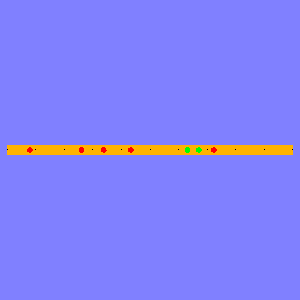
\includegraphics[height=5 cm]{figures/image16}
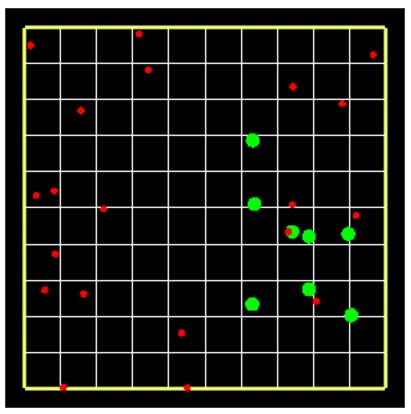
\includegraphics[height=5 cm]{figures/image17}
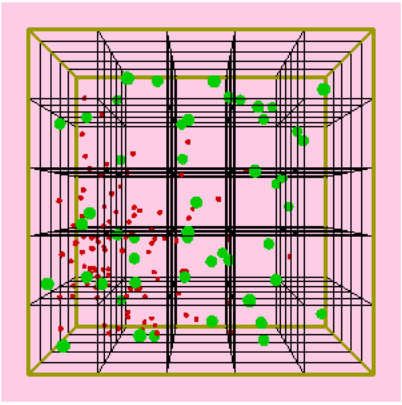
\includegraphics[height=5 cm]{figures/image18}
\caption{Output from graphics1.txt, graphics2.txt, and graphics3.txt showing some graphics options.}
\label{fig:graphics1}
\end{figure}

The following table lists the graphics statements

\begin{longtable}[c]{ll}
Statement & function\\
\hline\\
\ttt{graphics} $str$ & graphical output method\\
\ttt{graphic\_iter} $int$ & time steps run between renderings\\
\ttt{graphic\_delay} $float$ & additional delay between renderings\\
\ttt{quit\_at\_end} \ttt{yes/no} & Smoldyn should quit when it's done\\
\ttt{frame\_thickness} $int$ & thickness of system frame\\
\ttt{frame\_color} $color$ & color of system frame\\
\ttt{grid\_thickness} $int$ & thickness of virtual box grid\\
\ttt{grid\_color} $color$ & color of virtual box grid\\
\ttt{background\_color} $color$ & background color\\
\ttt{display\_size} $name float$ & size of display for a molecule species\\
\ttt{color} $color$ & color for a molecule species\\
\ttt{text\_color} $color$ & color for text display\\
\ttt{text\_display} $item$ & item that should be displayed with text\\
\ttt{tiff\_iter} $int$ & time steps between TIFF savings\\
\ttt{tiff\_name} $name$ & root name of TIFF files\\
\ttt{tiff\_min} $int$ & initial suffix for TIFF files\\
\ttt{tiff\_max} $int$ & largest possible TIFF suffix\\
\end{longtable}
The $color$ parameter can be either a color name, or the red, green, and blue color coordinates.

\section{Better graphics}

Smoldyn's better graphics, selected with the graphics \ttt{opengl\_better} statement, are intended to be adequate for publication-quality figures. With them, you can define a ``room'' light and up to 8 point lights. The room light is non-directional. Define its color with the \ttt{ambient} option. Each point light has a position and then colors for its ambient light, diffuse light, and specular light. To make the light position as a 3-dimensional point in space, enter 4 values for the position, and make the last value equal to 1. Alternatively, you can make the light directional but not arising from a specific position. To do this, keep all of the x, y, and z values between 0 and 1, and set the 4th value to 0. Ambient light is non-directional and does not reflect off of a surface. Diffuse light is directional (from the light source) but lights the illuminated side of a surface evenly, as though it is a non-shiny surface. Specular light is also directional and reflects off of a surface as though it is shiny.

Within each surface block, you can set the shininess of the surface with the \ttt{shininess} statement.


% Runtime commands
\chapter{Runtime commands}

\section{Command basics}

The design of a simulation can be broken down into two portions. One portion represents the physical system, including its boundaries, surfaces, molecules, and chemical reactions. These are the core components of Smoldyn and are simulated by the main program. The other portion represents the action of the experimenter, which include observations and manipulations of the system. As with the parameters of the physical system, these actions are also listed in the configuration file. They are listed as a series of commands and execution times.

There are no rules regarding what commands can and cannot do. Thus, in principle, commands could be used to measure any aspect of the simulated system at any time. Or, other commands could be used to manipulate any aspect of the system, regardless of whether the manipulations have any physical basis. In practice, there is a limited set of commands that have been written (listed below in the reference section) so the range of what can actually be done with commands is limited to what those in this list can do. Alternatively, a somewhat adventurous user can write his or her own source code to create a new command, as explained below. Because commands do not have to follow the rules that the rest of the code does, they are easy to add and are powerful, but they also tend to be less stable and less well optimized than the core program.

Commands are entered in a configuration file with the statement cmd, followed by some information about the execution timing, the specific command name, and finally any parameters for the command. Here are some examples:

\begin{lstlisting}[style=SSAC]
cmd b pause
cmd e ifno ATP stop
cmd n 100 molcount outfile.txt
\end{lstlisting}

The first one instructs the simulation to pause before it starts running, the second says that the simulation should stop if there are no molecules named ATP, and the third tells Smoldyn to print a count of all molecules to the file called outfile.txt every 100 iterations. In contrast to the statements that define the physical system, runtime commands are not parsed or interpreted until the simulation time when they are supposed to be executed. When a command is executed, Smoldyn processes it with a runtime command interpreter. If there are errors in command parameters, such as a missing or nonsensical parameter, these are not caught until the command is executed during the simulation.

Command execution timing works in either of two ways. A command can be performed at real-valued simulation times, such as before the simulation starts, at some particular time, or repeatedly at fixed time intervals. Alternatively, a command can be performed after some specified number of time steps. This avoids minor timing problems that can arise from round-off error. Commands for these two methods are stored in the continuous-time and integer command queues, respectively. If two commands are entered with the exact same timing instructions, then, at each invocation, they are performed in the same order as they are listed in the configuration file. On the other hand, the order may differ if their timing instructions differ; to be precise, they are executed in the order from the one that was least recently performed to the one that was most recently performed. If both integer and continuous time queue commands are supposed to execute at the same time step, then all of integer queue commands are performed first. Command timing is demonstrated with the configuration files S6\_commands/cmdtime1.txt and S6\_commands/cmdtime2.txt.

The following table shows the command timing options.

\begin{longtable}[c]{lll}
Code & parameters & execution timing\\
\hline\\
\multicolumn{3}{l}{continuous time queue}\\
\ttt{b} &  & runs once, before simulation starts\\
\ttt{a} &  & runs once, after simulation ends\\
\ttt{@} & $time$ & runs once, at $\geq time$\\
\ttt{i} & $on\ off\ dt$ & runs every $dt$, from $\geq on$ until $\leq off$\\
\ttt{x} & $on\ off\ dt\ xt$ & geometric progression\\
\multicolumn{3}{l}{integer queue}\\
\ttt{B} &  & runs once, before simulation starts\\
\ttt{A} &  & runs once, after simulation ends\\
\ttt{\&} & $i$ & runs once, at iteration $i$\\
\ttt{I} & $on_i\ off_i\ dt_i$ & runs every $dt_i$ iteration, from $\geq on_i$ to $\leq off_i$\\
\ttt{E} &  & run every time step\\
\ttt{N} & $n$ & runs every $n$ time steps
\end{longtable}

A few deprecated codes, which are in addition to the codes listed above, are that \ttt{j} is equivalent to \ttt{I}, \ttt{e} is equivalent to \ttt{E}, and \ttt{n} is equivalent to \ttt{N}. Although these are deprecated, they are commonly used, so they will probably be supported indefinitely.

Each command is one of three main types: control, observe, or manipulate. Control commands control the simulation operation. For example, a command called keypress, followed by a letter, causes the simulation to act as though that key had been pressed by the user. This can be useful for modifying the display automatically. Observation commands read information from the simulation data structures, analyze the data some, and output results to text files. The precision of numerical output values can be set using the \ttt{output\_precision} statement. Neither control nor observation commands modify any aspect of the simulation. Manipulation commands modify the simulation parameters, such as the addition, removal, or replacement of molecules, or the modification of reaction rate constants. These commands do not produce any output. Yet a fourth type of command is the conditional command. These test for certain simulation conditions, such as there being more than some number of some molecule species, and then run a second command if the conditions are met. Each conditional command is characterized as being one of the three main types based on the type of its second command.

\section{Output format and files}

Most observation commands output a series of data values. The default format is ``ssv'', which is space-separated vectors. These are easy for a person to read but are not as convenient when using most software. Thus, you can also use the \ttt{output\_format} statement to specify that you want ``csv'' output, which are comma-separated vectors.

For observation commands to work, one typically needs to declare the output file names with the statements \ttt{output\_files} or \ttt{append\_files}. The exception to this is if output should go to the standard output or standard error location, which are typically the terminal window. These are called ``stdout'' and ``stderr'', respectively, exactly as in C or C++. These can be declared with the \ttt{output\_files} statement but don't need to be.

To save output files in a subdirectory, the subdirectory path is declared with the \ttt{output\_root} statement. Note that the path needs to end with a ``/'', if you're working on a Mac or Linux system, or ``\\'' for Windows. This subdirectory path is concatenated on the end of the path that was used for the configuration file. It is possible to save a stack of files in which there is a separate file for each of many sequential observations. These are created with the \ttt{output\_file\_number} statement, which defines the starting suffix number for the file stack. Zero, which is the default, indicates no suffix number, whereas other numbers lead to a 3 digit suffix. The suffix number is incremented with the command incrementfile. The complete output filename is a concatenation of: the path for the configuration file, the string declared with \ttt{output\_root}, the file name declared with \ttt{output\_files} minus any suffix that starts with a ``.'', an underscore and the suffix number declared with \ttt{output\_file\_number}, and finally any suffix that starts with a ``.''. Here is an example, using Mac and Linux path notation:

\begin{longtable}[c]{ll}
working directory: & \ttt{theory}\\
configuration file: & \ttt{theory/expt1/myconfig.txt}\\
desired output files: & \ttt{theory/expt1/results/outfile\_001.txt}\\
 & \ttt{theory/expt1/results/outfile\_002.txt}\\
 & ...
\end{longtable}

Configuration file excerpt:
\begin{lstlisting}[style=SSAC]
output_root results/
output_files outfile.txt
output_file_number outfile.txt 1
cmd n 100 incrementfile outfile.txt
cmd e molcount outfile.txt
\end{lstlisting}
Starting Smoldyn: \ttt{smoldyn expt1/myconfig.txt}\\

Because of the potential for confusion with output file names, complete pathnames (relative to the working directory) are displayed at start-up with the simulation parameters.

An example that is essentially identical to the one shown above is in given in the example file S6\_commands/cmdfile.txt. Upon running it and looking at the results, you will discover that the first output file, cmdfileout\_001.txt, is empty, whereas all of the others are full, as expected. The empty file arises because the file number is incremented at the very beginning, before the molcount command is invoked for the first time. This could be remedied by using slightly more sophisticated command timing with the ``i'' or ``j'' timing codes.

\section{Specific commands}

All of the commands are listed below in the reference section, which is the definitive source of information about them. Most of the commands are also demonstrated in the example files S6\_commands/cmdobserve.txt and S6\_commands/cmdmanipulate.txt. Of the full list of commands, some are quite useful, some are rarely used, and some have been superceded by newer code. The last category includes several that implement rudimentary reflecting surfaces, which were written before a good treatment of surfaces was added to the core program. Of the more useful commands, a few deserve special mention.

The molcount command, and several variations of it, are used to save the numbers of each kind of molecule as a function of time. These are often the most useful text output commands from Smoldyn.
The savesim command causes the entire simulation state to be saved to a file as a configuration file that can be read by Smoldyn. With it, one can save a simulation mid-run and then continue running it later. This can be useful as a backup for intermediate results or for building starting states for complex simulations in several stages.

The keypress command creates an event that the program responds to, as though the user had pressed this key. For example, at the end of a simulation that uses graphics, the graphics window is left on the screen until the user selects quit from the menu or presses ``Q''. This quitting can also be programmed into the configuration file with ``cmd a keypress Q''. Arrows and other keypress options can be entered as well.

The set command enables you to enter essentially any configuration file statement mid-simulation. For example, the command \ttt{set species green} creates the species named ``green'' when the command is invoked, rather than at the beginning of the simulation. It's also possible to create surfaces, add reactions, etc. mid-simulation.

\section{Summary of statements about commands}

The following table summarizes the statements used for commands.

\begin{longtable}[c]{ll}
Statement & function\\
\hline\\
\ttt{output\_root} $str$ & root of path for text output\\
\ttt{output\_files} $str_1\ str_2\ �\ str_n$ & file names for text output\\
\ttt{output\_precision} $int$ & precision for numerical output\\
\ttt{append\_files} $str_1\ str_2\ �\ str_n$ & file names for text output\\
\ttt{output\_file\_number} $int$ & starting suffix number for file name\\
\ttt{output\_format} $str$ & output format; either ssv or csv\\
\ttt{cmd b,a,e} $string$ & command run times and strings\\
\ttt{cmd @} $time\ string$\\
\ttt{cmd n} $int\ string$\\
\ttt{cmd i} $on\ off\ dt\ string$\\
\ttt{cmd x} $on\ off\ dt\ xt\ string$
\end{longtable}


% Surfaces
\chapter{Surfaces}

\section{Surface basics}

A large fraction of biochemistry does not happen in free solution, but at or across cellular membranes. To model these interactions, Smoldyn supports surfaces within the simulation volume. Typically, one Smoldyn surface is used to model each type of membrane. For example, a bacterium might be modeled with one surface for the inner membrane and another for the outer membrane, while a eukaryotic cell would use separate surfaces for the plasma membrane, the nuclear membrane, and for each type of organelle. Smoldyn supports disjoint surfaces as well, such as for a collection of vesicles.

Each Smoldyn surface comprises many panels. These panels have simple geometries: for three-dimensional systems, a panel may be a rectangle, triangle, sphere, cylinder, hemisphere, or a disk. For one- and two-dimensional systems, lower dimensional analogs of these panel shapes can be used. There are two main reasons that Smoldyn supports this variety of primitive shapes rather than just the triangle meshes that are more common. First, these are much easier to use for simple models. For example, it is much easier to specify a simple spherical nucleus for a cell than it is to build an approximate sphere out of 20 or more triangles. Second, it is faster to simulate molecular collisions with one sphere or other simple curved objects than with a lot of triangles. In general, more geometric primitives are better. (Although, from the Smoldyn programmer's point of view, each one also requires a significant amount of math before it can be supported by Smoldyn).

Each surface includes a set of rules that dictate how molecules interact with it. This includes molecules that diffuse into it from solution, as well as molecules that are bound to the surface. All panels on a single surface interact with molecules in the same ways. Molecules that are bound to a surface are designed to represent membrane-bound proteins and trans-membrane proteins. For example, they can model signaling receptors or ion channels.

\section{Defining surfaces}

Surfaces are typically entered with one or more blocks of statements that start with \ttt{start\_surface} and end with \ttt{end\_surface}. Between these, only surface statements are recognized. A single surface may be broken up into multiple blocks of statements, and each block may describe multiple surfaces. The surface name may be given after the \ttt{start\_surface} statement, or it can be given afterwards with the name statement; this specifies which surface is being defined, and starts a new one if required.

As was mentioned before, Smoldyn surfaces do not work well in conjunction with the system boundaries that were defined with the boundaries, \ttt{low\_wall}, or \ttt{high\_wall} statements. If a configuration file includes any surface statement, even if no surfaces are actually defined, then all wall-type boundaries automatically behave as though they are transparent. To keep molecules within the system, an outermost surface needs to be defined. It may be a set of rectangular panels that are coincident with the system walls, a sphere that encloses the system, or something else. Molecules could also be allowed to escape the system although that is usually undesirable and can slow the simulation down (see below for the \ttt{unbounded\_emitter} statement, which provides an efficient alternative to escaping molecules).

The \ttt{action} or \ttt{rate} statements set the rules that molecules follow when they interact with a surface. For molecules in solution that collide with one of the surface faces, which are called front and back, there are three basic actions: reflection off of the surface, transmission through the surface, or absorption by the surface. It is also possible for a surface to be a ``jumping'' surface, such that if a molecule collides with it in one place, the molecule will be magically transported to a pre-defined destination. This is described below, as is another type of special surface called a ``porting'' surface. Yet another action option is ``multiple'', meaning that there any of several outcomes are possible and that there are specific rates for each. These rates are set with the rate statement (if rate is entered, the only possible action is ``multiple'', so the action statement may be omitted). For example, a membrane might be somewhat permeable to a molecular species, in which case one would set some rate for transmission; molecules that are not transmitted are reflected. Using the rate statement, it is also possible to cause a molecule to change species when it interacts with a surface. This is designed for molecules that behave sufficiently differently in different regions of space that it is most convenient to treat them with two different species; a typical use is for spatially-dependent diffusion coefficients.

The \ttt{action} and \ttt{rate} statements also apply to collisions of surface-bound molecules with other surfaces. This can arise when molecules diffuse along surfaces and two surfaces cross each other. For example, one way to create a lipid raft is to create a single surface for a cell membrane and then a short cylinder that intersects the membrane, creating an inner circular region and an other region (a Gaussian pillbox). Then, surface-bound molecules change species names when they cross the cylinder. An exception to the normal behavior arises when a surface-bound molecule collides with a panel that has been declared to be a neighbor of the molecule's panel. In this case, there are two options, which are selected with the \ttt{neighbor\_action} statement. The default behavior is that the molecule simply ignores the panel and diffuses through it. Alternatively, the molecule can be allowed to hop onto the new panel, with a 50\% probability of doing so. This latter possibility is helpful for allowing diffusion on a surface where the panels don't necessarily meet at their edges.

Sometimes, one wants a modeled system to be unbounded, such as for the simulation of pheromones that diffuse freely between cells, but that can also diffuse away towards infinity. While Smoldyn can simulate such unbounded systems with unbounded space, this can be very computationally intensive because it tracks every molecule, no matter how far it is from the region of interest. A better solution is to define a surface that surrounds the portion of the system that is of interest, where these surface panels absorb molecules at a rate that causes the system to behave as though it were unbounded. Smoldyn calculates this absorption rate automatically, from information that the user specifies with the \ttt{unbounded\_emitter} statement. This statement declares the positions and the production rates for each emission source within the simulation volume. The new absorption coefficients completely replace any other actions that might be defined for interactions between this surface and molecular species.

\section{Defining surface panels}

Individual surface panels are defined with one panel statement for each individual panel. These statements are used to specify panel locations, dimensions, orientations, and, sometimes, drawing information. Each panel also has a name, for which the default is simply the panel shape followed a number, although it is also possible for the name to be defined by the user at the end of the panel statement. These names are used for jumping surfaces and diffusion of surface-bound molecules. For a surface to work in a consistent manner, it is worth making sure that all panel front sides face the same way. The drawing information, such as the numbers of slices and stacks for a sphere, is only used for graphical rendering. As far as the simulation is concerned, a sphere, regardless of how it is drawn, is always a mathematically perfect sphere.

In general, panels should not be defined that are coincident with each other because this can lead to unreliable behavior. The rule is that if multiple panels are exactly coincident, whether they are members of the same surface or different ones, then only the one that is defined last in the configuration file is in effect. For example, one could define a washer-shaped surface using a large disk that reflects all molecules and a small disk, which has the same center and is parallel to the large disk, that transmits all molecules. However, computer round-off error often makes exact coincidence impossible; at best, it is most likely to work if the panels are parallel to the system axes or if they share the same center point. If two panels are very nearly but not exactly coincident (separations between 0 and $10^{-12}$ distance units), Smoldyn treats them as though they are reflective, which it has to do in order to prevent unintentional leaks where panels cross each other. Graphical rendering of coincident panels is unpredictable but rarely good.

Several configuration files were written to test the surface actions with all dimensions and all panel shapes. They are in the examples/S7\_surfaces directory and are called reflect\#.txt, transmit\#.txt, and absorb\#.txt, where the ``\#'' is 1, 2, or 3 for the system dimensionality. Additionally, the three surf\#.txt files show the basic actions in single files. Following is an excerpt from reflect3.txt, which shows how a surface and its panels can be defined:

\begin{lstlisting}[style=SSAC]
start_surface surf
action all both reflect
color both purple 0.5
thickness 2
polygon front face
polygon back edge
panel rect +0 40 40 40 20 20
panel rect -0 60 40 40 20 20
panel rect +1 40 40 40 20 20
panel rect -1 40 60 40 20 20
panel rect +2 40 40 40 20 20
panel rect -2 40 40 60 20 20
panel tri 60 15 70 80 15 70 70 15 86     # 1 2 3
panel tri 60 15 70 70 15 86 70 31 77     # 1 3 4
panel tri 70 15 86 80 15 70 70 31 77     # 3 2 4
panel tri 80 15 70 60 15 70 70 31 77     # 2 1 4
panel sph 20 20 20 8 20 20
panel cyl 20 75 20 80 75 80 5 20 20
panel cyl 20 30 70 20 50 70 4 20 20
panel hemi 20 75 20 5 1 0 1 20 20
panel hemi 80 75 80 5 -1 0 -1 20 20
panel disk 20 30 70 4 0 -1 0 20
panel disk 20 50 70 4 0 1 0 20
end_surface
\end{lstlisting}

Several statements control the drawing of surfaces to the graphics window. The \ttt{color} statement specifies the color of the front and/or back of the surface with either color words or red, green, blue, and alpha (opacity) values. As mentioned above in the graphics section, OpenGL does not render well with alpha values between 0 and 1. Thickness defines the line width that should be used for drawing surface edges, or for surfaces in 2-dimensional systems. The polygon statement is used to set the drawing mode for showing just the panel edges, only panel vertices, or complete panel faces. It also allows filling of regions for surfaces in 2-dimensions.

\section{Jumping surfaces}

There are a few situations in which one might reasonably want to have molecules move discontinuously, leaping from one place to another. One is for periodic boundaries in which molecules that diffuse off of one side of the system immediately diffuse onto the other side, thus keeping the composition of the system constant while avoiding effects that can arise from edges. Another situation is for building complex surface structures from the Smoldyn panel primitives without resorting to triangulated meshes. For example, one might want to have two spherical cells whose cytoplasms are linked by a narrow cylindrical channel, making a dumbbell shape. This would be easy to design in Smoldyn, except that there is no way to cut holes in the spheres where the cylinder should be attached. The solution is to put small disk-shaped ``jumping'' panels on each side of the spot where the hole is wanted so that molecules can be transported across the barrier (see examples/S7\_surfaces/dumbbell.txt).

To define a jumping surface, the action for each molecule that is to be jumped (usually set to all molecules, although fewer is permissible too), for the active face of the surface, is set to ``jump.'' Next, the active face of each panel needs to be assigned a destination panel and face using the jump statement. The source and destination panels are required to be the same shape and to be parallel to each other although, for certain shapes, they may differ in size.

Jumping surfaces are demonstrated with the files jump1.txt, jump2.txt, and jump3.txt, all in the S7\_surfaces directory.

Surface-bound molecules used to jump when they diffused onto panels that had surface-bound jump actions. However, this feature was removed in version 2.37 because it was complicated and there were better ways of accomplishing the same result.

\section{Membrane-bound molecules}

In Smoldyn, molecules can be in free solution or bound to surfaces. The bound ones can be attached on the front of the surface or on the back, called the ``front'' and ``back'' states, or they can be transmembrane molecules in either an ``up'' orientation or a ``down'' orientation. The precise meanings of these states are decided by the user. As an example, if a receptor is oriented such that the ligand binding site is on the outside of the cell, as usual, it could be called ``up,'' whereas if it were in the membrane in a reversed orientation, it could be called ``down.'' In all, there are five states that molecules can be in: ``solution,'' ``front,'' ``back,'' ``up,'' or ``down,'' of which the last four are the surface-bound states. In practice, all four surface-bound states are essentially equivalent. A molecule in any of these states is allowed to interact with solution-phase molecules that are on either side of the surface, and it can desorb to either side of the surface. The only real difference between these states is that Smoldyn ensures that molecules in the ``front'' state have coordinates that are slightly on the front side of the surface and those in the ``back'' state have coordinates that are slightly on the back side of the surface. Smoldyn does not fix the coordinates to be on any particular side for molecules in the ``up'' or ``down'' states, which makes these states simulate very slightly faster.

Additionally, it is sometimes necessary to specify the position of a solution-state molecule relative to a surface. For this, the pseudo-states ``fsoln'' (which is identical to ``solution'') and ``bsoln'' specify that it is solution state and on the front or back of the relevant surface.

The \ttt{surface\_mol} statement, which was mentioned in the section on molecules, is used to specify that there are molecules bound to a surface at the start of a simulation. The statement is quite versatile, allowing one to specify that molecules are scattered randomly over an entire surface, over specific panel shapes, over specific panels, or even over all surfaces. Also, of course, it is possible to specify exact molecule locations.

The \ttt{rate} statement, mentioned before in the context of partially permeable surfaces, is also used for transition rates for surface-bound molecules. It can be used for specifying the rate at which a solution-state molecular species is adsorbed onto a surface. It can also be used for the release rate, from surface to solution. In this situation, the release side of the surface is identified by giving the destination state as either ``fsoln'' or ``bsoln'', for the front and back, respectively. Rate is also used for transition rates between the different surface-bound states, such as from ``front'' to ``back.''

Surface-bound molecules diffuse within the plane of the surface according to the diffusion coefficient that was entered with the \ttt{difc} statement for the respective molecule state. To allow molecules to diffuse between neighboring surface panels, whether they are part of the same surface or different surfaces, these neighbors have to be declared with the \ttt{neighbors} statement. Diffusion on surfaces is reasonably quantitatively accurate, which is best understood with an explanation of the algorithm (most of which was new in version 2.37). Considering a three-dimensional system, a surface-bound molecule is initially diffused in all three dimensions. It is then moved back to the local plane of the panel that it is bound to. If this puts the molecule within the area of its panel, then the diffusion step is done and no further actions are taken. This approach is exact for flat panels and reasonably good for curved panels (and becomes exact in the limit of short time steps). If the new position is not within the area of the molecule's panel, Smoldyn determines where the line of the molecule's trajectory exits the current panel. Smoldyn then determines if there are other panels at this point (it actually checks for panels within an extremely small distance called $neighdist$ from this position, which is just large enough to prevent problems from computer round-off error). If so, it chooses one of these panels at random and rotates the molecule's trajectory that extends beyond the original panel into the plane of the new panel, thus preserving the length of the trajectory. If the end point of the new trajectory is within the new panel, then the diffusion step is done. If not, Smoldyn repeats the procedure until the trajectory is used up. Returning to a prior condition, if the molecule's trajectory leaves the molecule's current panel but there is no neighbor near the exiting point, then the molecule does not continue onto a neighbor. Instead, it reflects off of the panel edge, so that the trajectory continues on the original panel. This procedure should be exact for flat panels and extremely good for curved panels.

Note that molecules only transition from one panel to another when they diffuse off the edge of the initial panel. Thus, for example, a molecule can never diffuse off an edge of a sphere, with the result that molecules cannot diffuse from one sphere to another, even if these spheres intersect. If diffusion between panels is desired in these cases, then use the \ttt{neighbor\_action} statement, as described above. However, be forewarned that diffusion between neighboring panels can interact badly with the \ttt{neighbor\_action} hopping, which is why this hopping is turned off as a default. For example, suppose several 2D panels (which are lines) meet at a single point. A molecule diffusing along one of the panels correctly transitions to a new randomly chosen panel when it gets to that point. However, if \ttt{neighbor\_action} is set to hopping, then the trajectory during this transition might be discovered to cross yet another one of the panels in the process, so the molecule would then get moved onto this new panel. The probability of this outcome is biased by the precise panel positions and by round-off errors, with the result that the molecule position statistics would be incorrect.

Files that demonstrate surface-bound molecules are: S7\_surfaces/stick2.txt and cellmesh.txt (which reads cellmeshfile.txt). Surface diffusion is demonstrated with the files in S7\_surfaces/surfacediffuse/.

\section{Smoldyn bugs}

As far as I know, there are no bugs currently in Smoldyn that cause surfaces to behave other than requested. However, leaking surfaces have been a recurring problem with Smoldyn. In this problem, which can be caused by any of a vast number of small mistakes in the source code, molecules that shouldn't go through a surface are found to have done so. Some commands that were written to test for it are: \ttt{warnescapee} and \ttt{killmoloutsidesystem}. If you suspect that Smoldyn isn't working right, or if you just want to verify that it is working right (a good idea if you don't use graphical output), then it might be worth running these or other commands. The former one has to be run at every time step to be useful. The latter one has no output directly, but will identify problems if it is bracketed by \ttt{molcount} commands. The command \ttt{killmolinsphere} can be used in a similar manner.

\section{Statements about surfaces}

The following table summarizes the statements about surfaces.

\begin{longtable}[c]{ll}
Statement & function\\
\hline\\
\ttt{max\_surface} $int$ & (optional) maximum number of surfaces\\
\ttt{start\_surface} $name$ & start of a surface block\\
\ttt{name} $name$ & optional statement for the surface name\\
\ttt{action} $species(state)\ face\ action\ [new\_spec]$ & action for when a molecule contacts surface\\
\ttt{rate} $molec\ state_1\ state_2\ value\ [new\_spec]$ & transition rate\\
\ttt{neighbor\_action} $action$\\
\ttt{rate\_internal} $molec\ state_1\ state_2\ value\ [new\_spec]$\\
\ttt{color} face $color\ [alpha]$\\
\ttt{thickness} $float$\\
\ttt{polygon} $face\ drawmode$\\
\ttt{shininess} $face\ value$\\
\ttt{max\_panels} $char\ int$ & (optional)\\
\ttt{panel} $char\ float\ �\ float$\\
\ttt{panel} $char\ float\ �\ float\ name$\\
\ttt{jump} $name\ face\ ->\ name_2\ face_2$\\
\ttt{jump} $name\ face\ <->\ name_2\ face_2$\\
\ttt{neighbors} $panel\ neigh_1\ neigh_2\ �$\\
\multicolumn{2}{l}{
\ttt{unbounded\_diffusion} $face\ species\ amount\ pos_0\ pos_1\ �\ pos_{dim-1}$}\\
\ttt{end\_surface}
\end{longtable}

\section{Rates of surface interactions}

For an interaction to occur between a solution-state molecule and a surface, the molecule has to (1) contact the surface and (2) interact based on some probability. There are subtleties both in the determination of contacts and in the calculation of these probabilities.

Starting with the contacts, a molecule clearly contacted a surface during the preceding time step if it ended up across the surface from where it began, which I'll call a direct collision. It is also possible for a molecule to start and end on the same side of a surface, but to have contacted the surface at some point during the time step, labeled here as an indirect collision. The probability of an indirect collision occurring is (Andrews and Bray, Phys. Biol. 2004)
$$\exp\left({-\frac{l_1l_2}{D \Delta t}} \right)$$
Here, $l_1$ and $l_2$ are the perpendicular distances to the surface before and after the time step, $D$ is the diffusion coefficient, and $\Delta t$ is the time step. These indirect collisions are implemented in Smoldyn for simulating absorption of molecules to the bounding walls of the system (the boundaries).

However, for interactions between diffusing molecules and all surfaces, Smoldyn only accounts for direct collisions, thus ignoring the indirect collisions. This decreases the accuracy of Smoldyn slightly but is done because indirect collisions were found to be difficult to code, computationally demanding, and made essentially no difference to results.

The probability of interaction given that a collision has occurred is difficult to calculate. While it is presented in a recent paper by Erban and Chapman (Phys. Biol. 4:16-28, 2007) for adsorption interactions, their equation turns out to only be accurate in the limit of short time steps. Thus, I found the necessary relationships between the adsorption, desorption, or transmission coefficients and the corresponding adsorption, desorption, and transmission probabilities. They are implemented in the SurfaceParam.c source code file of Smoldyn and have been thoroughly tested. I plan to write these algorithms up and submit them for publication during the next few months.

The adsorption coefficient, $\kappa$ has units of length/time. The product $\kappa c$, where $c$ is a concentration (units of length$^{-3}$), is the adsorption rate in molecules adsorbed per unit of time, per unit of surface area. If the surface is in equilibrium with the solution, where there is a sticking coefficient of $\kappa$, and an unsticking rate of $k$, then the equilibrium surface density of molecules is
$$C_{surface} = \frac{\kappa}{k} C_{solution}$$
Surface sticking rates were tested with the example file stickrate.txt. Here, a collection of molecules diffuses freely in solution, but sticks with rate 0.5 on one side. This situation can be solved analytically as well from equations in Crank, allowing for a good comparison. Comparison between simulation and theory are shown in the figure below.

\begin{figure}[h]
\centering
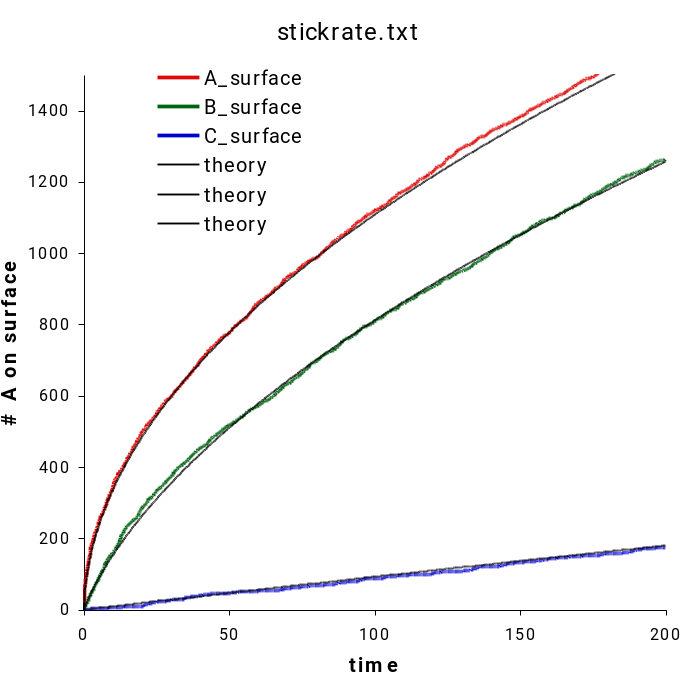
\includegraphics[height=5 cm]{figures/image21}
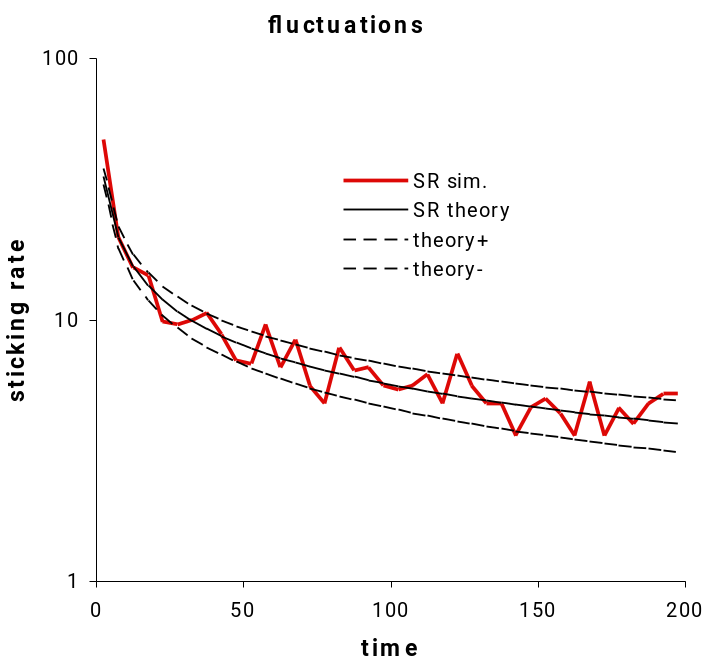
\includegraphics[height=5 cm]{figures/image22}
\caption{Output from stickrate.txt, showing quantitatively accurate adsorption.}
\label{fig:stickrate}
\end{figure}

Results from example stickrate.txt, shown in red, are compared with the analytic solution for the sticking rate. The left panel shows the total number of molecules stuck to the surface. The right panel shows the average sticking rate with a 5 time unit averaging window, with comparisons to the expectation sticking rate shown with a solid line and the 1 standard deviation range shown with dashed lines.

\section{Simulating effective unbounded diffusion}

The example files in S7\_surfaces/unbounded\_diffusion illustrate and verify the use of a partially absorbing bounding surface to simulate effective unbounded diffusion. These files use the Smoldyn file sphere.txt, which describes a sphere; I created it by using Mathematica to define a sphere, triangulate it, and save it as a ``wrl'' (Virtual Reality Modeling Language) file. Then, I used the wrl2smol utility program to convert it to the Smoldyn-readable file sphere.txt. Other Smoldyn configuration files specify either one or multiple emitters within this sphere and then save concentration line profiles as functions of time. The theoretical concentration distributions for these situations is expressed with a slight extension of eq. 3.5b from Crank, which leads to
$$C(\mathbf{r}) = \sum_i \frac{q_i}{4 \pi D |\mathbf{r} - \mathbf{r}_i} \erfc \frac{|\mathbf{r}-\mathbf{r}_i |}{2 \sqrt{Dt}}$$
Here, $C(\mathbf{r})$ is the concentration at position $\mathbf{r}$, $q_i$ is the emission rate of source $i$, $D$ is the diffusion coefficient, $\mathbf{r}_i$ is the location of source $i$, and $t$ is the time since the sources started emitting. At steady-state, this concentration equation simplifies to
$$C(\mathbf{r}) = \sum_i \frac{q_i}{4 \pi D |\mathbf{r} - \mathbf{r}_i} $$ 
The figure below shows results from the emitter1.txt Smoldyn simulation, in which an emitter at location $\mathbf{r}_1 = (-4.5,0,0)$ microns emits $q_1 = 500$ molecules per second, these molecules have a diffusion coefficient of $D = 3 \mu \textrm{m}^2/\textrm{s}$, and the system is surrounded by a triangulated sphere that is centered at the origin and has radius 10 microns. Absorption to this sphere was set to make the molecules diffuse as though the system were unbounded. Close agreement between simulation and theory show that the algorithm works well.

\begin{figure}[h]
\centering
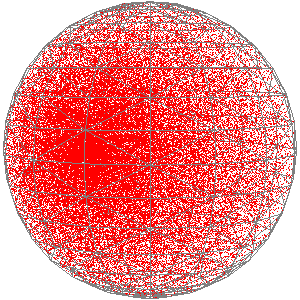
\includegraphics[height=4 cm]{figures/image25}
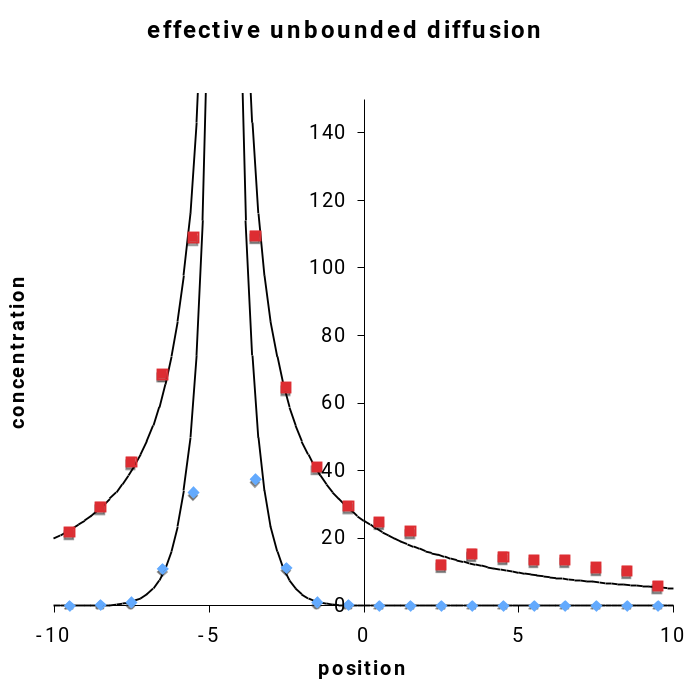
\includegraphics[height=5 cm]{figures/image26}
\caption{Output from emitter1.txt, showing quantitatively accurate effective unbounded diffusion.}
\label{fig:emitter1}
\end{figure}

The left panel shows a snapshot from example emitter1.txt where it is seen that the emitter center is somewhat left of the sphere center and the sphere is triangulated. The right panel shows line profiles across the middle of the sphere, from (-10,0,0) to (10,0,0) at times $t = 0.3$ s (blue) and $t = 100$ s (red), with simulation data shown with points and theoretical results, from the equations above, in solid lines.


% Reactions
\chapter{Reactions}

\section{Reaction basics}

There are three types of chemical reactions in Smoldyn: zeroth order, first order, and second order, where the order is simply the number of reactants. Synonyms for the latter two are unimolecular and bimolecular reactions. In addition, Smoldyn simulates a couple of additional interaction types using reactions; these are conformational spread reactions and excluded volume reactions, both of which are described below.

With zeroth order reactions, there are no reactants at all. Instead, products appear spontaneously at random locations in the system volume (or within a compartment) at a roughly constant rate. This is unphysical because particles are being created from nothing. However, since Smoldyn explicitly ignores many chemical species, the assumption here is that some unmodeled chemicals are being converted into the zeroth order product. Thus, it is assumed that there is a legitimate underlying chemical reaction that produces the products that are seen, but it just isn't part of the model. (At least, this is the typical use of zeroth order reactions; using them to model the magical production of matter is fine too.)

First order reactions involve the conversion of one molecular species into another. This includes spontaneous conformational changes of proteins and chemical rearrangements of small molecules. Also, many reactions are pseudo-first order, meaning that one of two reactants has a sufficiently constant concentration and distribution that it can be left out of the model and its effect is lumped into the rate constant of a first order reaction. Protein phosphorylation by ATP is a good example of this. In Smoldyn, reactants of first order reactions have a certain probability of converting to products at each time step.

Second order reactions occur when two reactants collide and react (conformational spread reactions are an exception, as described below). In Smoldyn, a reaction radius is defined for each pair of molecular species. For those that do not react with each other, the reaction radius is 0. For those that can react, the reaction radius is some small distance on the order of the molecular radii, with values that increase monotonically with the standard mass action reaction rate. To simulate each time step, molecules are first diffused and then, typically, all reactant pairs that are closer than their reaction radii are reacted. Thus, the stochasticity in simulated bimolecular reactions arises solely from diffusion and not from the reaction step of the algorithm. It is also possible for the reaction probability upon collision to be some value less than one if desired, which can be useful for adjusting the extent to which a reaction is diffusion- or activation-limited.

If a reaction has multiple products, they are usually all added to the system at the same point. They can also be separated from each other by a small amount, called the unbinding radius if there are two products, which reduces the likelihood of their immediate recombination in a new reaction. This recombination is called a geminate recombination.

It is possible to specify that a reaction should only occur within a spatial compartment (defined below), or if one of the reactants is bound to a specified surface. For example, it is possible to declare that a zeroth order reaction should only produce product within a specific compartment, or that a first order reaction is only active when the reactant is within the specified compartment. In many cases, these rules are unphysical, although they can be very useful for treating interactions with spatially localized unmodeled chemical species. These restrictions can slow down simulations, so only use them if they are needed.

Conformational spread reactions are only intended to be used with stationary reactants and are only permitted in reactions with two reactants and two products. A conformational spread reaction is possible if the reactants are closer together than the conformational spread radius, which is analogous to the binding radius of normal second order reactions (although its value is constant, regardless of the time step). For a conformational spread reaction, the reaction rate has units of inverse time, as it is for a first order reaction. If a reaction occurs, the first entered reactant is replaced by the first product, and the second reactant with the second product.
Excluded volume reactions use the reaction concept to simulate excluded volume interactions. Here, the typical reaction is of the form A + B $\rightarrow$ A + B, with the ``binding radius'' set to the sum of the physical molecular radii and the product placement type set to ``bounce''. There are several options for simulating these reactions. The default and usually best approach is called the reflection method. Here, if molecules are found to be within a binding radius after diffusion, their positions are recomputed by reflecting the molecules off of each other based upon their straight-line trajectories during the course of the time step; the collision point is at the position along the trajectories where the center-to-center distance equals the binding radius. A different approach is the overlap method. Here, if molecules are found to be closer than their binding radius after diffusion, then the distance by which they are closer is added to the binding radius to compute the new separation. The molecules are separated by this amount, while keeping the molecule centers on the same line as they were on before they were moved.

Each molecule has a serial number that can be used to uniquely identify it. In most reactions, the reactants are simply removed from the system and the reaction products are new molecules with new serial numbers. However, this is not the case for conformational spread and excluded volume reactions because the reactants and products are conceptually the same molecules, so these products have the same serial numbers as the reactants. It can also be helpful to maintain serial numbers in other situations, such as for single molecule tracking. In these situations, use the \ttt{reaction\_serialnum} statement to define rules for the product serial number assignments.

\section{Defining reactions}

To define a reaction, enter the statement reaction, followed by the reaction name, the reaction, and the rate constant. Here are some examples:

\begin{lstlisting}[style=SSAC]
reaction r1 A + B -> C 10
reaction bind receptor(up) + ligand(fsoln) -> complex(up) 1
reaction ingest complex(up) -> receptor(up) + ligand(bsoln) 5
reaction tca 0 -> ATP 100
reaction decay fluorophore(all) -> 0 0.01
\end{lstlisting}

For molecule states that are not specified, as in the first example above, it is assumed that the reaction only applies to molecules that are in solution. Reactions that only occur in specified compartments are entered in the same way, but with the \ttt{reaction\_cmpt} statement. Versions of Smoldyn prior to 1.82 allowed reactions to be entered in definition blocks; this is still permitted for backward compatability, but is discouraged because this format is not being maintained and may be eliminated in future versions.

For most applications, the \ttt{reaction} statement is sufficient for entering the reaction rate. However, other methods are possible as well. It is possible to leave the rate constant off of the reaction line and enter it separately with the statement \ttt{reaction\_rate}. The reaction rate is the macroscopic reaction rate, which is converted into parameters that Smoldyn can use for the simulation. For zeroth order reactions, the reaction rate is converted to the average number of molecules that should be added to the entire simulation volume at each time step. To enter this internal value directly, use the statement \ttt{reaction\_production}. For first order reactions, the reaction rate is converted to the probability that a reactant molecule will react during one time step. This can be entered directly with the statement \ttt{reaction\_probability}. For second order reactions, the reaction rate is converted into a reaction binding radius, which can be entered directly with \ttt{binding\_radius}.

If a reaction has multiple products, they are usually placed at the location where the reaction was determined to have occurred. However, offsets from the reaction location are possible as well, which are necessary for reversible reactions so as to avoid certain geminate recombinations. Offsets can be entered directly or can be calculated by Smoldyn in many different ways. All of them are entered with the \ttt{product\_placement} statement.

Conformational spread reactions are a special type of bimolecular reactions. For these, there is a domain of interaction, which is entered with the statement \ttt{confspread\_radius}; this also specifies that the reaction uses conformational spread. Reaction rate constants for conformational spread reactions have units of inverse time, like a first order reaction rate constant. They indicate the rate at which a reaction occurs, for reactants that are continuously closer to each other than the conformational spread radius. As with first order reactions, this rate value is converted to a reaction probability at each time step, and can be entered directly with the \ttt{reaction\_probability} statement. The two products of conformational spread reactions are placed at the exact same locations as the two reactants, using the same ordering of reactants and products as they are listed with the reaction statement.

To simulate second order reactions with reaction probabilities that are not equal to one (called the lambda-rho algorithm), you can set the reaction probability with the \ttt{reaction\_probability} statement. Alternatively, you can set the reaction $\chi$ value, which is the ratio of the actual reaction rate constant to the diffusion-limited reaction rate constant, using \ttt{reaction\_chi}.

\section{Statements about reactions}

The following table summarizes the statements about reactions.

\begin{longtable}[c]{l}
Statement\\
\hline\\
\ttt{reaction} $rname\ reactant_1\ +\ reactant_2\ ->\ product_1\ +\ product_2\ rate$\\
\ttt{reaction} $rname\ reactant_1\ +\ reactant_2\ <->\ product_1\ +\ product_2\ rate_{fwd}\ rate_{rev}$\\
\ttt{reaction compartment}$=cname\ rname\ reactant_1\ +\ reactant_2\ ->\ product_1\ +\ product_2\ rate$\\
\ttt{reaction surface}$=sname\ rname\ reactant_1\ +\ reactant_2\ ->\ product_1\ +\ product_2\ rate$\\
\ttt{reaction\_rate} $rname\ rate$\\
\ttt{confspread\_radius} $rname\ radius$\\
\ttt{binding\_radius} $rname\ radius$\\
\ttt{reaction\_probability} $rname\ prob$\\
\ttt{reaction\_chi} $rname\ chi$\\
\ttt{reaction\_production} $rname\ value$\\
\ttt{reaction\_serialnum} $rname\ rules\_list$\\
\ttt{product\_placement} $rname\ type\ parameters$
\end{longtable}

\section{Reactions with a block format}

Although now discouraged and deprecated, the block format for entering reactions is similar. The block starts with the statement \ttt{start\_reaction} and ends with \ttt{end\_reaction}, between which only instructions that are relevant to reactions are allowed. The first statement within a reaction block is order to define the reaction order of this block. The \ttt{max\_rxn} statement used to be required next, but is no longer functional as of version 1.82. Basic reactions are entered with a \ttt{reactant} statement, a \ttt{rate} statement, and a \ttt{product} statement. It is also possible to enter the internal value that Smoldyn uses with \ttt{rate\_internal}. It is possible to turn states on or off with the \ttt{permit} statement. If there are multiple products, and if these products can react with each other (most often a reversible reaction), then Smoldyn may need some information about the product unbinding radii, which is entered with the \ttt{product\_param} statement. It is discussed at length below.

Conformational spread reactions are slightly different. Enter the conformational spread radius with the \ttt{confspread\_radius} statement and the reaction rate (which is analogous to a first order rate) with rate. This rate value is converted to a reaction probability at each time step. To enter the latter value directly, do so with the \ttt{probability} statement. The \ttt{rate\_internal} statement is ignored.

\section{Zeroth order reactions}

Zeroth order reactions have no reactants and yet produce products at a rate that is constant except for stochastic fluctuations. They can be used to simulate the production of molecules that are of interest from sub-systems that are not of interest and thus are not explicitly part of the model. As mentioned above, zeroth order reactions have not proven to be particularly useful.
The zeroth order reaction 0 $\rightarrow$ A proceeds according to the mass action rate equation
$$\frac{d[\textrm{A}]}{dt} = k$$
$k$ is the reaction rate constant. Solving for the number of A molecules in volume $V$ as a function of time yields the deterministic solution
$$n(t) = n(0)+kt$$ 
$n(0)$ and $n(t)$ are the initial and time-dependent numbers of A molecules. There are also fluctuations due to the stochastic nature of chemical processes. Smoldyn assumes that each molecule created in a zeroth order reaction is created independently of each other, which allows Poisson statistics to be used. As an example of a limitation, this is not a perfect description of biochemical protein production because that involves sequential stochastic DNA transcription followed by many relatively rapid mRNA translations, thus leading to stochastic bursts of protein production.

Zeroth order reactions were tested with the file zeroreact.txt. The reaction portion of the configuration file is

\begin{lstlisting}[style=SSAC]
reaction slow 0 -> red 0.001
reaction med 0 -> green 0.01
reaction fast 0 -> blue 0.1
\end{lstlisting}

As seen in the figure below, simulation results conform closely to corresponding theoretical results, using a wide range of reaction rates. As expected, stochastic deviations from the deterministic theoretical predictions are seen.

\begin{figure}[h]
\centering
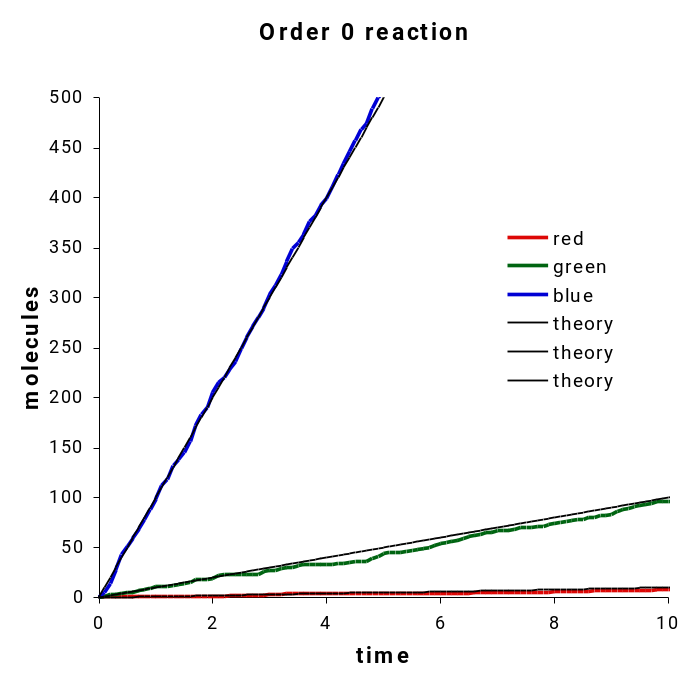
\includegraphics[height=5 cm]{figures/image29}
\caption{Output from zeroreact.txt, showing quantitatively accurate zeroth order reactions.}
\label{fig:zeroreact}
\end{figure}

This shows zeroth order reaction molecule production with data simulated from the example file S8\_reactions/zeroreact.txt. Shown are the numbers of molecules produced as a function of time with three different production rates along with the deterministic theory for how many molecules would be expected.

\section{Unimolecular reactions}

Order 1 reactions follow the general reaction equation A $\rightarrow$ B. The mass action kinetics for the loss of reactant are described with the differential equation
$$\frac{d[\textrm{A}]}{dt} = -k [\textrm{A}]$$ 
where $k$ is the first order reaction rate. This is solved to yield the deterministic solution for the number of A molecules as a function of time,
$$n(t) = n(0) e^{-kt}$$ 
n(0) is the number of A molecules at time 0 and n(t) is the number at time t.

The example file S8\_reactions/unireact1.txt was used to check unimolecular reaction rates using a wide range of reaction rates. The reaction portion of the configuration file is

\begin{lstlisting}[style=SSAC]
reaction slow red -> 0 0.1
reaction med green -> 0 1
reaction fast blue -> 0 10
\end{lstlisting}
As seen in the figure below there is good agreement between simulation and theory. As always, stochastic fluctuations are apparent, which is particularly true when there are few molecules.

First order reactions in which a reactant can react through multiple possible pathways requires slightly more complicated calculations for the reaction probabilities. However, the mass action differential equation, shown above, is unchanged. This situation was tested with the configuration file unireactn.txt. The reaction portion of the configuration file is

\begin{lstlisting}[style=SSAC]
reaction r1 A -> A + B 0.1
reaction r2 A -> A + C 0.05
reaction r3 A -> A + D 0.01
\end{lstlisting}
The system is started with only A molecules, so the theoretical number of A molecules as a function of time is
$$n_A(t) = n_A(0) e^{-(k_B+k_C+k_D)t}$$
The number of B molecules as a function of time is
$$n_B(t) = n_A(0) \frac{k_B}{k_B+k_C+k_D} \left[1-e^{-(k_B+k_C+k_D)t} \right]$$
Analogous equations hold for C and D. Simulation results closely matched these theoretical equations, as shown in the figure below.

\begin{figure}[h]
\centering
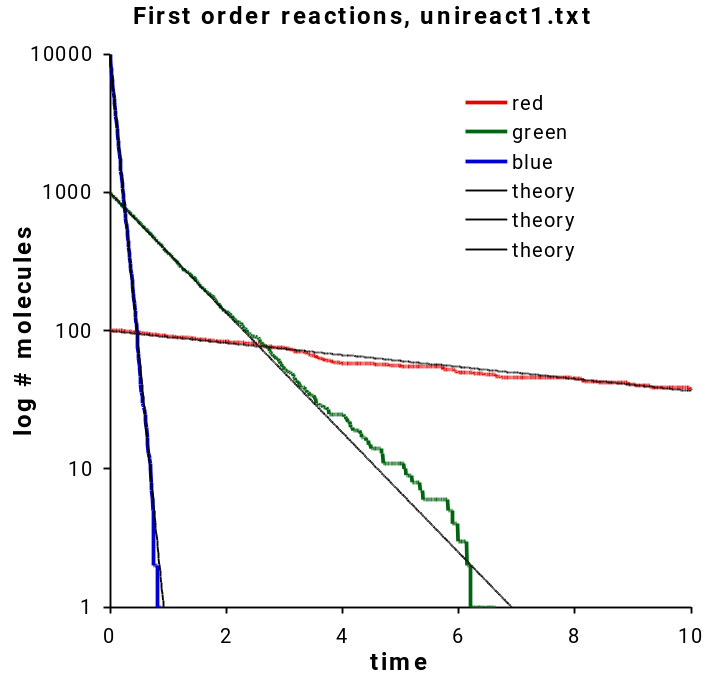
\includegraphics[height=5 cm]{figures/image34}
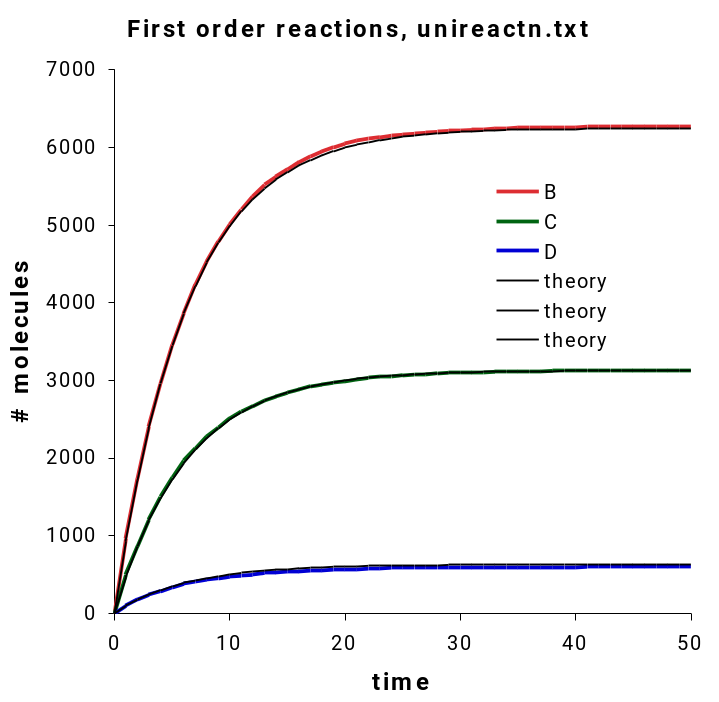
\includegraphics[height=5 cm]{figures/image35}
\caption{Output from unireact1.txt and unireactn.txt, showing quantitatively accurate first order reactions.}
\label{fig:unireact1}
\end{figure}

The panel on the left shows results from the configuration file unireact1.txt. First order reactions occur at rates that are in good agreement with theory over a wide range of rate values. The panel on the right shows results from the file unireactn.txt. Again, there is good agreement with theory.

\section{Bimolecular reactions}

Bimolecular reactions have the generic reaction equation A + B $\rightarrow$ C, for which the mass action kinetics are described by the deterministic differential equations
$$\frac{d[\textrm{A}]}{dt} = \frac{d[\textrm{B}]}{dt} = -\frac{d[\textrm{C}]}{dt} = -k [\textrm{A}] [\textrm{B}]$$
The reaction rate constant, $k$, is only actually constant if: (i) the reaction kinetics are purely activation-limited, or (ii) the reaction has proceeded long enough that a steady-state reactant distribution has formed.

This equation is not quite as trivial to solve as prior ones were. With the condition that there are the same numbers of A and B molecules initially, the solution for the number of A molecules (or B molecules) as a function of time is
$$n(t) = \left(\frac{1}{n(0)} + \frac{kt}{V} \right)^{-1}$$
As before, $n(0)$ is the initial number of A or B molecules, $n(t)$ is the number of A or B molecules as a function of time, $k$ is the reaction rate constant and $V$ is the volume of the system. This was tested with three different reaction rates with the configuration file reactAB.txt, for which the reaction portion of the file is

\begin{lstlisting}[style=SSAC]
reaction slow As + Bs -> Cs 1
reaction med Am + Bm -> Cm 10
reaction fast Af + Bf -> Cf 100
\end{lstlisting}
The Smoldyn diagnostics output shows how these different reaction rates are converted into simulation parameters. They are converted into binding radii, which is small for the slow reaction and large for the fast reaction. Because the reaction kinetics depend on the ratio of the reactant rms steps lengths to the binding radii, the slow one has relatively long steps compared to the binding radius and thus behaves as though it is activation-limited. In contrast, the fast reaction has short rms step lengths compared to the binding radius and so behaves as though it is diffusion-limited. Shortening the simulation time step would make all of these more diffusion-limited.

Activation-limited reactions follow the mass action kinetics shown in the equations for all times. Thus, the slow and medium reaction rate simulations agree well with the mass-action theory, as shown in the figure, below. In contrast, the diffusion-limited simulation does not agree with the mass-action theory. This is because the simulation starts with molecules randomly distributed whereas the analytical result assumes a steady-state distribution. However, after enough time has passed for a steady state reactant distribution to be formed, it is shown that the simulated results agree well with the analytical results (orange line in the figure).

\begin{figure}[h]
\centering
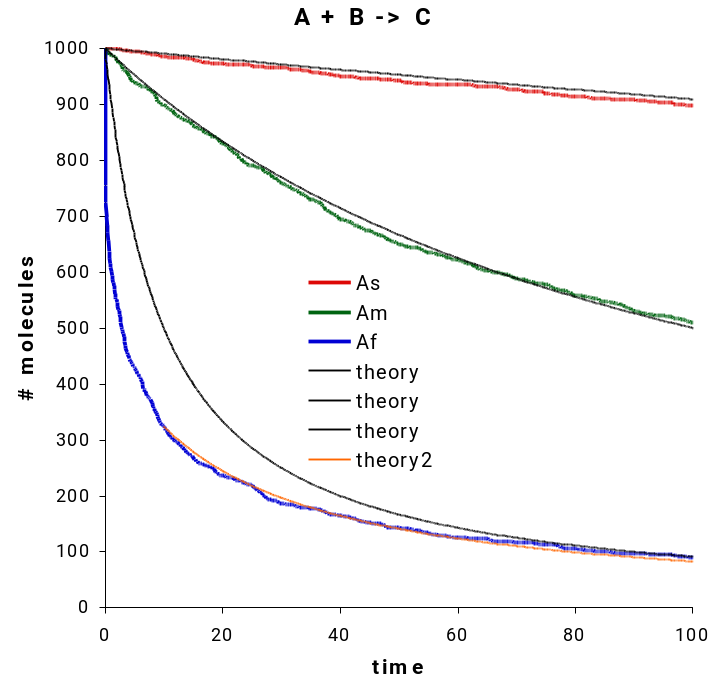
\includegraphics[height=5 cm]{figures/image38}
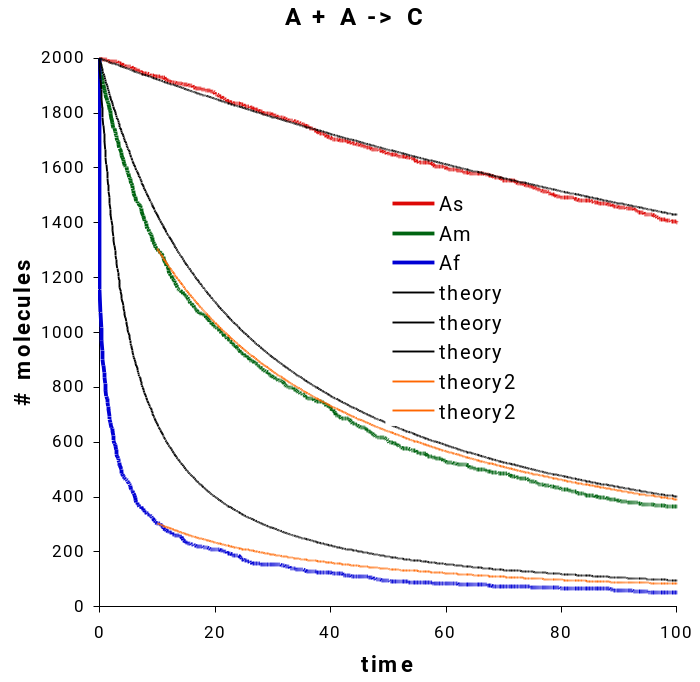
\includegraphics[height=5 cm]{figures/image39}
\caption{Output from bireactAB.txt and bireactAA.txt, showing quantitatively accurate second order reactions.}
\label{fig:bireactAB}
\end{figure}

The panel on the left shows reactant numbers for the reaction A + B $\rightarrow$ C for three different reaction rates and with equal initial numbers of A and B molecules. The panel on the right is similar but for the reaction 2A $\rightarrow$ C. Light black lines are solutions to the deterministic steady-state mass action rate equations. Deviations arise for the faster reactions (blue lines) because those start far from steady-state. Light orange lines are the steady-state theory, starting with time 10 rather than 0, so as to start at times when reactants are closer to steady-state distributions.

\section{Reactions with identical reactants}

Although there are no conceptual or simulation algorithm differences for bimolecular reactions in which two reactants are the same, there are a few quantitative differences. Consider a situation with 1000 A molecules and 1000 B molecules. Despite the fact that each A molecule has about 1000 potential collision partners, whether the reactants are A + A or A + B, there are twice as many A-B collisions as A-A collisions. This is because each A-A pair can be counted in either of two ways, but is still only a single possible collision. To achieve the same reaction rate for A + A reactants as for A + B, despite the fact that there are fewer collisions, Smoldyn uses a larger binding radius for the former.

The analytical solution for the number of A molecules as a function of time is also slightly different from before,
$$n(t) = \left(\frac{1}{n(0)} + \frac{2kt}{V} \right)^{-1}$$
The reaction description portion of the configuration file S8\_reactions/bireactAA.txt is

\begin{lstlisting}[style=SSAC]
reaction slow As + As -> C 1
reaction med Am + Am -> C 10
reaction fast Af + Af -> C 50
\end{lstlisting}
Results are similar to those seen before. Simulation results agreed well with the analytical equations if the reaction is activation-limited or once the reactant distributions have reached steady-state, but agreement is not good for diffusion-limited reactions away from steady-state. It should be emphasized that these discrepancies are not errors by Smoldyn, but are quite the opposite: they are approximations made in the steady-state equations which people are used to making but which are nevertheless incorrect, which are being compared to accurate simulations by Smoldyn.

\section{Diffusion-limited reactions}

Diffusion-limited reactions can be simulated well by Smoldyn. The example file bireactABB.txt again simulates the reaction A + B $\rightarrow$ C, but now with a lot more B molecules than A ones, and with a time step that is sufficiently short that the reaction simulates as though it is diffusion-limited. As is shown in the figure below, results conform closely to the Smoluchowski prediction for this reaction.

\begin{figure}[h]
\centering
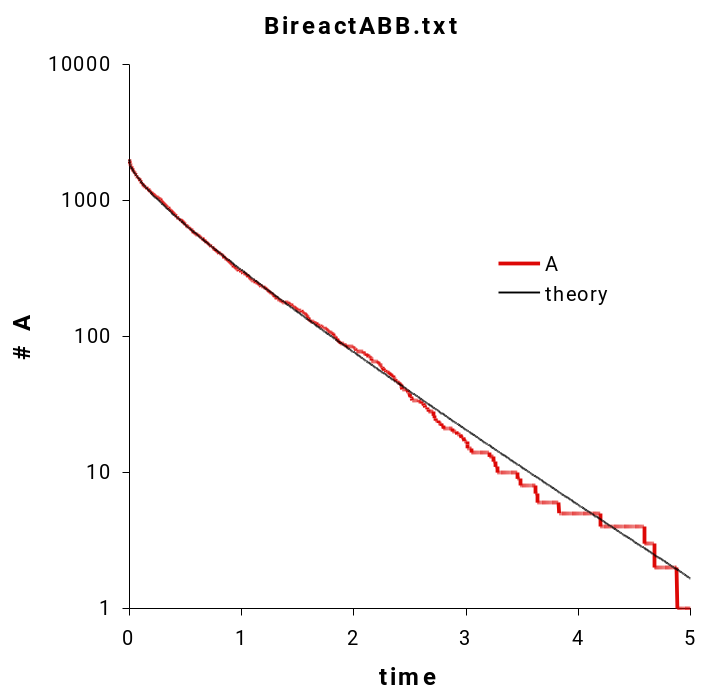
\includegraphics[height=5 cm]{figures/image41}
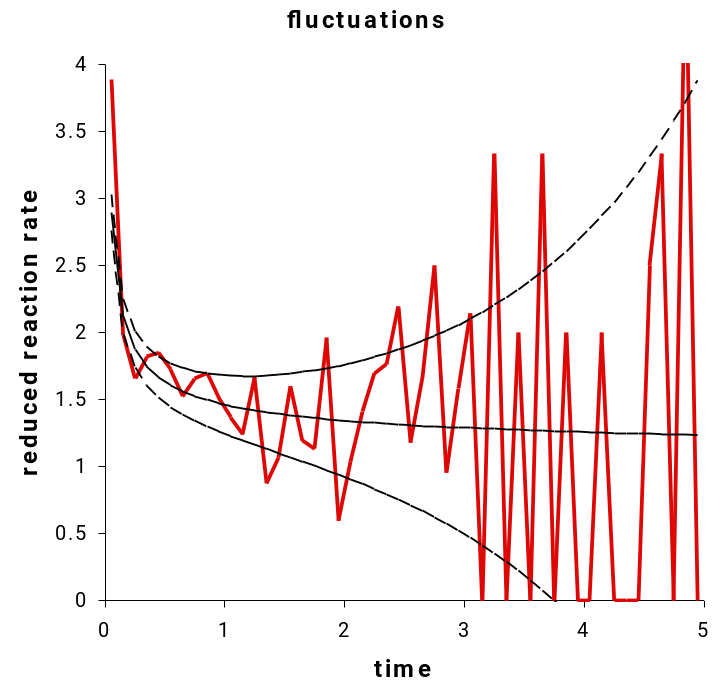
\includegraphics[height=5 cm]{figures/image42}
\caption{Output from bireactABB.txt, showing accurate diffusion-limited reactions.}
\label{fig:bireactABB}
\end{figure}

This example shows diffusion-limited bimolecular reactions from the configuration file bireactABB.txt, which simulates the reaction that is described in Figure 7 of Andrews and Bray, 2004. The left panel shows the number of surviving A molecules as a function of time with comparison to the time-dependent Smoluchowski equation. The right panel shows the reaction rate per A molecule per time unit as a function of time along with the Smoluchowski prediction with the solid black line and predicted fluctuations with the dashed lines.

\section{Reversible reactions}

Reversible reactions, where at least one has multiple products, involve geminate recombination issues, as discussed below. The accuracy of reversible reaction rates using the default reverse parameter type and parameter was investigated with the configuration file S8\_reactions/equil/equil.txt. Here, an equilibrium is set up for the reaction A + B $\leftrightarrow$ C.

From standard chemistry, the equilibrium constant is related to the ratio of product to reactant concentrations and to the ratio of the forward to reverse rate constants,
$$K=\frac{n_C V}{n_A n_B} = \frac{k_f}{k_r}$$
where $V$ is the total system volume. The configuration file equil.txt starts with equal numbers of A and B molecules and no C molecules. Using the above equation and this starting point, the solution for the equilibrium number of A molecules is
$$n_A = \frac{-V + \sqrt{V^2+4Kn_A(0) V}}{2K}$$
where $n_A(0)$ is the initial number of A molecules. It was verified that the simulation result approached this value.

\begin{figure}[h]
\centering
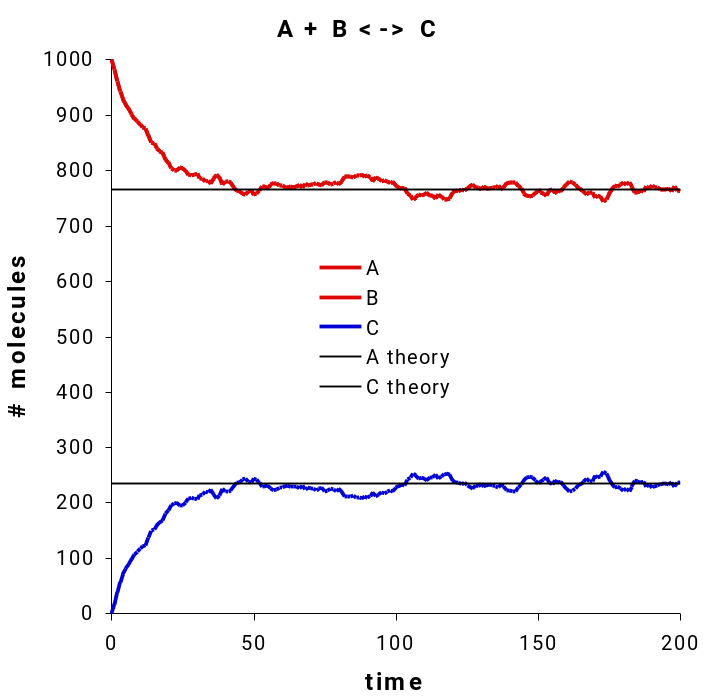
\includegraphics[height=5 cm]{figures/image45}
\caption{Output from equil.txt, showing accurate reversible reactions and equilibrium.}
\label{fig:equil}
\end{figure}

This figure shows the equilibrium result from example file S8\_reactions/equil/equil.txt.

\section{Multi-step reactions}

Many biochemical models include reactions that do not fall neatly into the 0th, 1st, or 2nd order reaction categories, but are instead complex reactions that include multiple elementary steps. Whereas these complex reactions can be well-defined for models that are either deterministic or non-spatial, they simply don't make sense when individual molecules are modeled. Thus, to include them in a Smoldyn model, one has to explicitly define each of the steps.

Taking the Michaelis-Menten reaction as an example, consider substrate S, enzyme E, and product P. The full reaction system is

All three of these reactions, along with the enzyme-substrate complex ES, need to be defined in a Smoldyn file. Of course, this means that you also need to give the three reaction rate constants $k_1$, $k_{-1}$, and $k_2$. Assume you know the Michaelis constant $K_M$ and the maximum reaction velocity $V_{max}$. As can be found in any biochemistry textbook, these are connected to the underlying rate constants as
$$K_M = \frac{k_{-1} + k_2}{k_1} \qquad V_{max} = k_2 [\textrm{E}]_0$$
where $[\textrm{E}]_0$ is the total enzyme concentration. These two equations are not sufficient to solve for the three rate constants, so let us define the unitless reaction efficiency ratio, $r$, as the fraction of ES that goes to P,
$$r=\frac{k_2}{k_{-1}+k_2}$$
This value can range between 0 and 1, where small values represent rapid equilibration between E, S, and ES, and high values represent rapid reaction of ES to P. Typical Michaelis-Menten analyses assume the former situation, so we might guess that $r$ is 0.1. Solving these equations for the reaction rate constant yield:
$$k_1 = \frac{V_{max}}{[\textrm{E}]_0 K_M r} \qquad k_{-1} = \frac{V_{max} (1-r)}{[\textrm{E}]_0 r} \qquad k_2 = \frac{V_{max}}{[\textrm{E}]_0}$$
Other multi-step reactions can be broken down to elementary reactions in a similar manner. The need to include additional assumptions, as we did here with $r$, is typical when converting from a low-detail reaction rate equation to a high-detail reaction mechanism.

\section{Reaction networks}

The reaction types presented above can be combined to create essentially unlimited varieties of reaction networks. A particularly simple one is shown here as an example. It is the classic Lotka-Volterra reaction network, which was originally designed to explain observed oscillations in ecological predator-prey systems but is also analogous to many natural biochemical oscillators. The terminology used here borrows from the ecology application, although all numbers were chosen solely to make for an interesting simulation result. The complete file S8\_reactions/lotvolt/lotvolt.txt is:

\begin{lstlisting}[style=SSAC]
# Simulation file for Lotka-Voltera reaction

graphics opengl
graphic_iter 5

dim 3
names rabbit fox
max_mol 20000
molperbox 1

difc all 100
color rabbit 1 0 0
color fox 0 1 0
display_size rabbit 2
display_size fox 3

molecule_lists rlist flist
mol_list rabbit rlist
mol_list fox flist

time_start 0
time_stop 100
time_step 0.001

boundaries x -100 100 p
boundaries y -100 100 p
boundaries z -10 10 p

mol 1000 rabbit u u u
mol 1000 fox u u u

cmd b pause
#output_files lotvoltout.txt
#cmd i 0 5 0.01 molcount lotvoltout.txt

reaction r1 rabbit -> rabbit + rabbit 10
reaction r2 rabbit + fox -> fox + fox 8000
reaction r3 fox -> 0 10

end_file
\end{lstlisting}

This involves several statements that make the simulation run efficiently. Graphics are only displayed every 5 iterations, the simulation is set up with only 1 molecule per virtual box, and the rabbit and fox molecules are stored in separate molecule lists. Results from this file are shown in the figure below.

\begin{figure}[h]
\centering
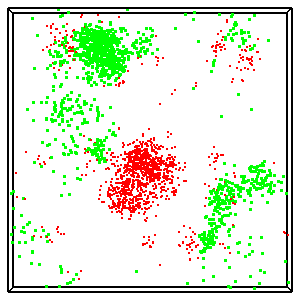
\includegraphics[height=5 cm]{figures/image53}
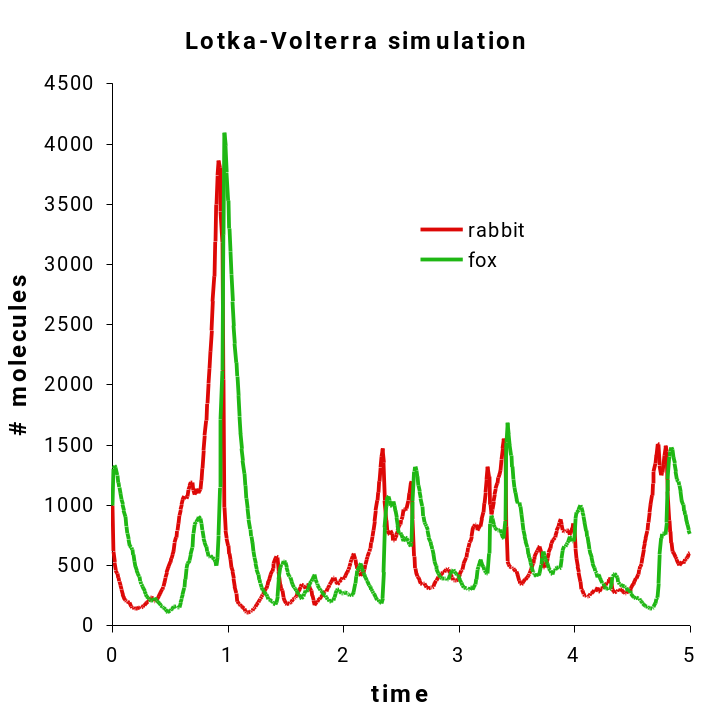
\includegraphics[height=5 cm]{figures/image54}
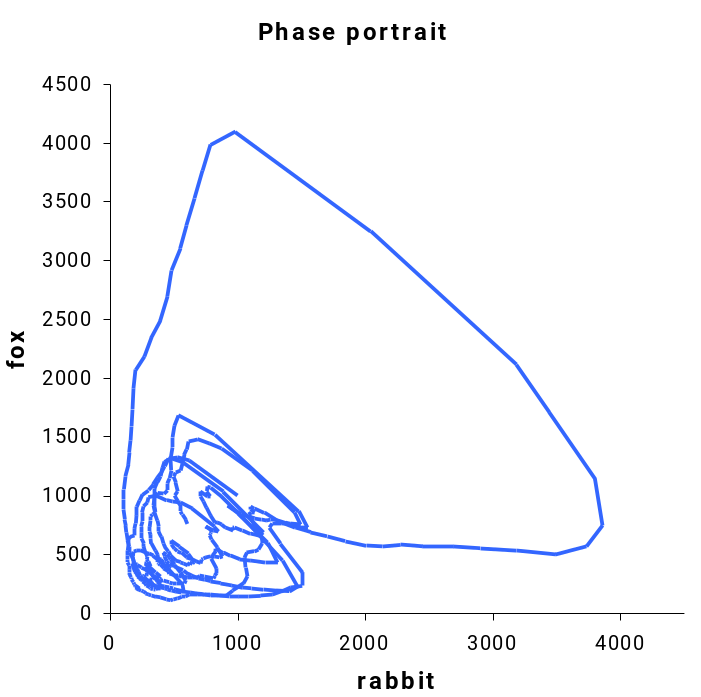
\includegraphics[height=5 cm]{figures/image55}
\caption{Output from lotvolt.txt, showing a simple reaction network with Lotka-Volterra dynamics.}
\label{fig:lotvolt}
\end{figure}

These figures show results from Lotka-Volterra simulation. The first panel shows of snapshot of the simulation after it has run for long enough for the regular boom-and-bust pattern to develop. Red dots are ``rabbits'' and green dots are ``foxes''. The next panel shows the numbers of ``rabbit'' and ``fox'' molecules as a function of time, with the same colors, again illustrating the boom-and-bust pattern. The panel on the right is a phase portrait of the data shown in the center; oscillations lead to cycles in the phase portrait and the initial large spike is seen as the large diameter cycle.

\section{Conformational spread reactions}

Currently, Smoldyn only allows second order reactions that have exactly two products to be declared a conformational spread reaction. Defining them as a conformational spread reaction, which is done with the \ttt{confspread\_radius} statement, implies a few things. Typically, the diffusion coefficients of both reactants are zero, although this is not required. The reaction rate constant that is entered is a \textit{first order} rate constant, meaning that it has units of inverse time. It is interpreted as the rate at which a reaction will occur, given that both reactants are continuously closer to each other than the conformational spread radius. Finally, the products of a conformational spread reaction are placed in the exact same locations as the reactants, and in the spots that correspond to the order in which the reactants and products were listed in the configuration file. For example, consider the conformational spread reaction defined with the statements
\begin{lstlisting}[style=SSAC]
reaction rxn1 A + B -> C + D 10
confspread_radius rxn1 5
\end{lstlisting}
This states that a conformational spread reaction can occur between any A and B molecules that are closer than 5 distance units apart. At each time step, the probability of its occurring is found from the reaction rate of 10 inverse time units according to the same formulae that were described above for unimolecular reactions. If it occurs, the A molecule will be replaced by a C molecule and the B molecule will be replaced with a D molecule.

Conformational spread processes are frequently symmetric such that activity can be spread from an active molecule to its neighbor, and also inactivity can spread from an inactive molecule to its neighbor. This can be entered in Smoldyn with a pair of conformational spread reactions:
\begin{lstlisting}[style=SSAC]
reaction rxna inactive + active -> active + active 10
reaction rxni active + inactive -> inactive + inactive 10
confspread_radius rxna 5
confspread_radius rxni 5
\end{lstlisting}
This will yield a warning in Smoldyn about there being multiple bimolecular reactions listed with the same reactants, but it is the right way to list these symmetric effects. In this example, the convention was followed that the latter reactant (and latter product) is the neighbor molecule, while the former reactant is the one that changes state.

If a molecule has simultaneous conformational spread interactions with more than one other molecule, the simulated reaction rates may be too low; this effect is reduced to zero for short time steps and increases with longer time steps. Consider a potential reaction with two reaction channels and the probability of it happening by either channel individually is $p$. When the two channels are considered sequentially, the probability for the first happening should be p, while the probability for the second should $p/(1p)$, because it is the conditional probability of the second reaction happening, given that the first one did not happen. However, Smoldyn uses probability $p$ for all conformational spread reaction channels, which leads to a reaction rate that is too low. While this identical effect is addressed correctly for first order reactions and for state conversions of surface-bound molecules, it is not addressed for conformational spread reactions because it is nearly impossible for Smoldyn to figure out how many reaction channels are available for any particular conformational spread reaction.

Conformational spread reactions were tested with the configuration file confspread.txt. It simulates two reactions:
\begin{lstlisting}[style=SSAC]
reaction back green -> red 10
reaction fwd red + blue -> green + blue 10
confspread_radius fwd 5
\end{lstlisting}
While it is simplistic for most conformational spread situations, it leads to a simple equilibrium between red and green molecules which allows for easy analytical calculations of the correct outcome. If each red/green molecule is within a conformational spread radius of one blue molecule (accomplished by setting the conformational spread radius to 3), the forward and reverse rates are each 10 and an equal number of red and green molecules should be observed. On the other hand, an increased conformational spread radius (5, as shown above) implies that each red/green molecule is within reach of two blue molecules, so the forward rate doubles, as does the equilibrium constant. Both of these behaviors were confirmed. As described above, conformational spread reaction probabilities that were greater than about 0.05 for each reaction led to conformational spread reaction rates that were observed to be slightly too low for the case in which each red molecule was within the conformational spread radius of two blue molecules.

\begin{figure}[h]
\centering
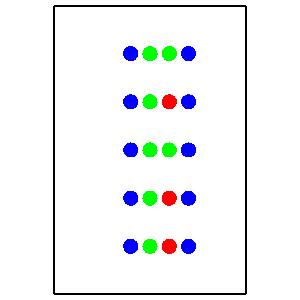
\includegraphics[height=5 cm]{figures/image56}
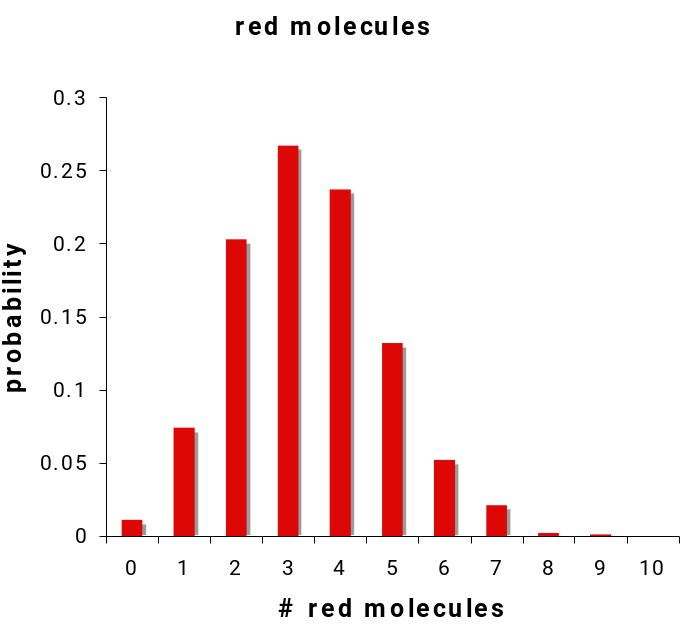
\includegraphics[height=5 cm]{figures/image57}
\caption{Output from confspread.txt, showing accurate conformational spread interactions.}
\label{fig:confspread}
\end{figure}

This figure show output from confspread.txt configuration file. There are conformational spread reactions between blue molecules and red molecules, which convert red to green; reversion is a simple reaction. The panel on the right shows the average probability of molecules being in their red states, for a situation in which rate constants are equal for the forward and reverse reactions, but each red/green molecule is within a conformational spread radius of two blue molecules, thus doubling the red $\rightarrow$ green reaction rate.

\section{Excluded volume reactions}

Smoldyn can treat molecules as though they have excluded volume using the same reaction concept that was developed for bimolecular reactions. The user specifies the collision radius (using the \ttt{binding\_radius} statement) for each pair of species that is supposed to respect each others' excluded volume and then makes this an excluded volume reaction with the \ttt{product\_placement} statement, with the bounce option. If molecules of those two species end up within their collision radius at the end of a time step, they are then moved apart. The reactants and products may be the same molecular species, in which case the molecules are simply pushed apart. They can also be different species. Molecules maintain their serial numbers. There are several options for the \ttt{product\_placement} parameter value. Setting it to a positive value (which should be larger than the binding radius) causes the two products to be placed at this distance apart, along the same vector as the molecules were on before they were moved apart. Setting it to -1 is generally more accurate; here, the products are separated by the binding radius plus the distance that the reactants had been inside of the binding radius. This separation is along the vector that separated the reactants. Setting it to -2, or leaving the value blank because this is the default method, is better yet. Here, the molecules bounce ballistically off of each other. This is the most accurate method. In all cases, the reaction rate value is largely meaningless for excluded volume reactions.

If molecules are not supposed to pass by each other, which can be simulated using excluded volume reactions and a one-dimensional system, then it is important to make the excluded volume binding radius significantly larger than the rms step lengths of the molecules. Because molecules move during diffusion with Gaussian-distributed displacements, and Gaussians have long tails, it is likely to be very difficult to ensure that absolutely no molecules cross that should not.

I illustrate excluded volume reactions with several examples, all of which are in the S8\_reactions/bounce directory. In one, bounce.txt, molecules are confined to a line and maintain their ordering. The configuration file statements that declare the excluded volume reactions are:
\begin{lstlisting}[style=SSAC]
reaction rxn1 red(up) + green(up) -> red(up) + green(up)
binding_radius rxn1 1
product_placement rxn1 bounce -2
\end{lstlisting}
A second example involves a crowded system and is in the same directory and the file crowding.txt.

\begin{figure}[h]
\centering
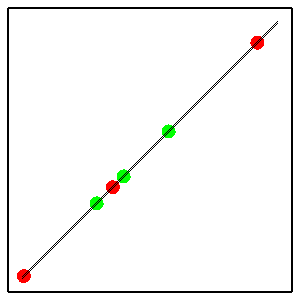
\includegraphics[height=5 cm]{figures/image58}

\includegraphics[height=5 cm]{figures/image59}
\caption{Output from bounce.txt and crowding.txt, showing excluded volume for surface-bound and solution phase molecules.}
\label{fig:crowding}
\end{figure}

These figures show output from bounce.txt and crowding.txt. In the former, red and green molecules, both of which are confined to the diagonal line, bounce off of each other. This has the result that the ordering of red and green molecules does not change during the simulation. The latter file shows that this crowding method works even with relatively high molecule densities. These molecules clearly do not overlap each other. During the simulation, molecules diffuse within the confines set by their neighbors.

\section{Binding and unbinding radii}

For every bimolecular reaction, Smoldyn has to calculate the correct binding radius from the reaction rate that is given in the configuration file. Also, for every reaction that leads to multiple products, Smoldyn has to determine the correct unbinding radius, using whatever product parameter is supplied, if any. Product parameters are listed in the table, below. While these binding and unbinding radii are well defined microscopic parameters (at least within the context of the Smoluchowski model system that is simulated), the meanings of the experimental rate constants, including those given in the configuration file, are not nearly as well defined. Instead, those rate constants depend on the conditions under which they were measured. Smoldyn accounts for this by attempting to guess the experimental conditions, using a process described here. If Smoldyn's guess is correct, the simulated reaction rates should exactly match the experimental rates (not including edge effects, which are typically negligible unless one reactant is fixed at or near an edge).

The following table shows product parameters for reactions with multiple products.

\begin{longtable}[c]{lll}
\multicolumn{3}{l}{Special product types}\\
\ttt{i} & \ttt{irrev} & reaction is declared irreversible ($\sigma_u=0$).\\
\ttt{a} & \ttt{confspread} & conformational spread reaction (entered automatically for you).\\ \\
\multicolumn{3}{l}{Use these if reversible reactions were measured at equilibrium}\\
\ttt{p} & \ttt{pgem} & probability of geminate reaction ($\phi$).\\
\ttt{x} & \ttt{pgemmax} & maximum probability of geminate reaction ($\phi_{max}$).\\
\ttt{r} & \ttt{ratio} & unbinding radius relative to binding radius ($\sigma_u/\sigma_b$).\\
\ttt{b} & \ttt{unbindrad} & fixed length unbinding radius ($\sigma_u$).\\ \\
\multicolumn{3}{l}{Use these if reversible reactions were measured with all product removed as it was formed}\\
\ttt{q} & \ttt{pgem2} & probability of geminate reaction ($\phi$).\\
\ttt{y} & \ttt{pgemmax2} & maximum probability of geminate reaction ($\phi_{max}$).\\
\ttt{s} & \ttt{ratio2} & unbinding radius relative to binding radius ($\sigma_u/\sigma_b$).\\
\ttt{o} & \ttt{offset} & fixed offset of products, rotationally randomized ($\sigma_u$).\\
\ttt{f} & \ttt{fixed} & fixed offset of products, not rotationally randomized ($\sigma_u$).
\end{longtable}

Either the single-letter code or the full word may be used to define the product parameter type, although the latter is suggested for readability. The default type is \ttt{pgemmax} with a value of 0.2.

In all cases, Smoldyn assumes that rate constants were measured using an effectively infinite number of reactant molecules, in an infinite volume, that were started well mixed and that then were allowed to react until either an equilibrium was reached for reversible reactions, or a steady-state reaction rate was reached for irreversible reactions. Only in these cases is mass action kinetics correct and is the reaction rate constant actually constant. The precise experimental assumptions are clarified with the following examples.

\begin{description}
\item{1. A + B $\rightarrow$ C}

The rate constant is assumed to have been measured at steady state, starting with a well-mixed system of A and B. No product parameter is required. At steady-state, the simulation matches mass action kinetics.

\item{2. X $\rightarrow$ A + B}

There is no bimolecular reaction, so no binding radius is calculated. The default unbinding radius is 0, although it is possible to define a different one. If the product parameter type is \ttt{pgem}, \ttt{pgem2}, \ttt{ratio}, or \ttt{ratio2}, an error is returned due to the lack of a binding radius. If the parameter type is not given or is \ttt{irrev}, \ttt{pgemmax}, or \ttt{pgemmax2}, the unbinding radius is set to 0. If it is \ttt{unbindrad}, \ttt{fixed}, or \ttt{offset}, the requested separation is used. At steady-state, the simulation matches mass action kinetics.

\item{3. A + B $\leftrightarrow$ C}

If the reversible parameter is \ttt{pgem}, \ttt{pgemmax}, \ttt{unbindrad}, or \ttt{ratio}, the forward rate constant is assumed to have been measured using just this system of reactions after the system had reached equilibrium. The product parameter is used to yield the correct probability of geminate recombination if possible, or the desired unbinding radius. In this case, the simulation matches mass action kinetics at equilibrium. If the product parameter is \ttt{pgem2}, \ttt{pgemmax2}, \ttt{ratio2}, \ttt{offset}, \ttt{fixed}, or \ttt{irrev}, then it is assumed that the forward rate constant was measured at steady-state and with all C removed as it was formed, thus preventing any geminate reactions. The unbinding radius is set as requested, using the binding radius if needed. In this case, the simulated forward reaction rate is higher than requested due to geminate rebindings.

\item{4. A + B $\leftrightarrow$ C $\rightarrow$ Y}

The second reaction is ignored for determining parameters for A + B. Instead, the first reaction is considered as though the rates were determined experimentally using just the system given in example 3. If the product parameter is \ttt{pgem}, \ttt{pgemmax}, \ttt{ratio}, or \ttt{unbindrad}, the simulated reaction rate for the forward reaction A + B $\rightarrow$ C will be lower than the requested rate because there are fewer geminate reactions than there would be with the equilibrium system. Alternatively, it will be higher than the requested rate if the product parameter is \ttt{pgem2}, \ttt{pgemmax2}, \ttt{ratio2}, \ttt{offset}, \ttt{fixed}, or \ttt{irrev}, because there are some geminate reactions.

\item{5. X $\rightarrow$ A + B $\leftrightarrow$ C}

The binding radius for the second reaction is treated as in example 1, without consideration of the first reaction. The unbinding radius for the first reaction is found using the binding radius of the second reaction. Here, product parameters \ttt{pgem} and \ttt{pgem2} are equivalent, \ttt{pgemmax} and \ttt{pgemmax2} are equivalent, and \ttt{ratio} and \ttt{ratio2} are equivalent. The actual reaction rate for the second reaction, found with a simulation, will be higher than the requested value due to geminate rebindings that occur after the dissociation of X molecules.

\item{6. X $\rightarrow$ A + B $\leftrightarrow$ C}

The A + B $\leftrightarrow$ C binding and unbinding radii are treated as in example 3. Another unbinding radius is required for the first reaction, which is found as in example 5, using the binding radius from the second reaction. Mass action kinetics are not followed.

\item{7. X $\leftrightarrow$ A + B $\leftrightarrow$ C}

The binding radii and unbinding radii for each bimolecular reaction are found as in example 3, independent of the other bimolecular reaction. The simulated rates may be different from those requested because of differing unbinding radii.

\item{8. X $\rightarrow$ A + B $\rightarrow$ C,   A + B $\rightarrow$ D}

The binding radii for the two bimolecular reactions are each found as in example 1. The unbinding radius for the first reaction cannot be determined uniquely, because the two forward reactions from A + B are equivalent and are likely to have different binding radii. Smoldyn picks the binding radius for the first forward reaction that is listed. Thus, if the product parameter for dissociation of X is \ttt{pgem}, the requested geminate rebinding probability will be found for the reaction A + B $\rightarrow$ C, but a different value will be found for the reaction A + B $\rightarrow$ D.

\item{9. C $\leftrightarrow$ A + B $\leftrightarrow$ C}

This reaction scheme might represent two different pathways by which A and B can bind to form an identical complex. However, Smoldyn cannot tell which reverse reaction corresponds to which forwards reaction. Instead, for both determining the binding and unbinding radii, it uses the first reverse reaction that is listed.
\end{description}

The general principle for calculating binding radii is that Smoldyn first looks to see if a reaction is directly reversible (i.e. as in example 3, without any consideration of reaction network loops or other possible causes of geminate reactions). If it is and if the reversible parameter is \ttt{pgem}, \ttt{pgemmax}, \ttt{ratio}, or \ttt{unbindrad}, then the binding radius is found under the assumption that the rate constant was measured using just this reaction, at equilibrium. If not, or if the reversible parameter is \ttt{pgem2}, \ttt{pgemmax2}, \ttt{ratio2}, \ttt{offset}, \ttt{fixed}, or \ttt{irrev}, then Smoldyn calculates the binding radius with the assumption that the rate constant was measured using just that reaction at steady-state and with all product removed as it is formed.

Unbinding radii typically require a reversible parameter (except as in example 2). If the parameter is \ttt{unbindrad}, \ttt{offset}, or \ttt{fixed}, the requested unbinding radius is used. If it is irrev, the unbinding radius is set to 0. Otherwise, it can only be calculated with the knowledge of the binding radius. If the reaction is directly reversible, the binding radius for the reverse reaction is used. If it is not directly reversible but the products can react, as in examples 5, 6, and 8, then the binding radius for the first reaction that is listed is used.

\section{Bimolecular reactions and surfaces}

Does a bimolecular reaction occur if there is a surface between the reactants? This turns out to be a somewhat complex question. The simple answer is that it does occur if the surface is transparent to both molecular species and it does not occur if the surface is reflective or absorptive to both molecular species. In principle, reactions should be possible across pairs of jump surfaces, although they are not performed by the current Smoldyn version which treats jump surfaces as though they are opaque with respect to reactions.

Smoldyn determines where the reaction location is using a weighted average of the reactant diffusion coefficients. The reaction takes place only if both reactants can get to the reaction position, considering any intervening surfaces. Absorption on the opposite side of a surface is not worried about, the logic being that molecules are already in contact when a reactant traverses the surface, and so opposite-side absorption is no more important than the reaction. For partially transparent surfaces, reactions occur depending on the probability of transparency.

When molecules have excluded volume, which they do not in Smoldyn, even inert impermeable surfaces can affect the local concentrations of chemicals. An obvious effect is that a molecule cannot be closer to a surface than its radius, leading to a concentration of zero closer than that. In a mixture of large and small molecules, Brownian motion tends to push the large molecules up against surfaces while the small molecules occupy the center of the accessible volume, thus creating more complex concentration effects. These effects do not occur when excluded volume is ignored, as it is in Smoldyn, in which case surfaces do not affect local concentrations.

While surfaces do not affect concentrations of non-reacting molecules, they do affect reaction rates. Consider the reaction A + B ? C, where A is fixed and B diffuses. If essentially all A molecules are far from a surface, the diffusion limited reaction rate is found by solving the diffusion equation for the radial diffusion function (RDF) with the boundary conditions that the RDF approaches 1 for large distances and is 0 at the binding radius (see the paper by myself and Dennis Bray titled ``Stochastic simulation of chemical reactions with spatial resolution and single molecule detail''). This leads to the Smoluchowski rate equation
$$k=4 \i D \sigma_b$$
However, for an A molecule that is near a surface, an additional boundary condition is that the gradient of the 3 dimensional RDF in a direction perpendicular to the surface is zero at the surface. This makes the solution of the reaction rate sufficiently difficult that I have not attempted to solve it, but the result is different from the simple result given above. This surface effect is an issue whenever the A molecule is within several binding radii of a surface and is especially pronounced when it is closer to the surface than its binding radius. For cases in which the A molecule is more than one binding radius from the surface, B molecules are going to take longer than usual to reach the region between the A and the surface, leading to a decreased reaction rate. It is suspected that the reaction rate decreases monotonically as the A molecule approaches and then crosses a surface.

A special case that can be solved exactly occurs when the A molecule is exactly at the surface, such that half of the binding volume is accessible to B molecules and half is inaccessible. Now, the RDF inside the system volume is identical to the RDF for the case when the A molecule is far from a surface. The logic is to assume that this is true and to then observe that it already satisfies the additional boundary condition. Using this RDF, the diffusive flux is half of the diffusive flux for an A molecule far from a surface, because only half of the binding surface is exposed to the system. Thus, the diffusion limited reaction rate for the situation in which a reactant is fixed exactly at a surface is
$$k = 2 \pi D \sigma_b$$

The situation changes some when simulation time steps are sufficiently long that rms step lengths are much longer than binding radii. Now, the probability of a reaction occurring during a time step is a function of only the binding volume. Thus, there are no surface effects at all when an A molecule is fixed anywhere in the simulation volume that is greater than or equal to one binding radius away from a surface. As the A molecule is moved closer to the surface, the reaction rate decreases in direct proportion to the binding volume that is made inaccessible to B molecules. An especially easy situation is that when the A molecule is exactly at the surface, the reaction rate is half of its value when the A molecule is far from a surface, which is the same as the diffusion limited result.

These results can be turned around to solve for the binding radius. If the reaction is diffusion limited, the binding radius should double when a reactant is placed exactly at the surface to maintain the same reaction rate. If it is activation limited, the binding radius should increase by $\sqrt[3]{2}$ to maintain the same reaction rate. As usual though, the binding radius is more closely related to the fundamental physical properties of the molecule than is the rate constant, so it is essential to consider the experimental conditions that were used for measuring the rate constant.

In conclusion, reaction rates are reduced near surfaces and the effect is different for diffusion limited and activation limited reactions. However, for both cases, and almost certainly for all cases in between, the reaction rate is exactly half when an A molecule is fixed at a surface, compared to when it is far from a surface. A few tests with Smoldyn using the files wallreact.txt, suggested that these surface effects are likely to be minimal for most situations, although it is good to be aware of their potential. The exception is that there are large surface effects when molecules are fixed with a significant portion of the binding volume outside the simulation volume.


% Compartments
\chapter{Compartments}

\section{Compartment basics}

Compartments are regions of volume that are bounded by surfaces. In general, they do not include their bounding surfaces. Compartments are useful for input or output and, as mentioned above, zeroth and first order reactions can be made to be only active within specified compartments. Compartments can also be moved around using various commands, thus providing support for moving surfaces. In addition, compartments are used for communication with the MOOSE simulator.

The inside of a compartment is defined to be all points from which one can draw a straight line to one of the ``inside-defining points'' without crossing any bounding surface. For example, to create a spherical compartment, one would define a spherical surface as the boundary and some point inside the sphere (the center, or any other internal point) to be the inside-defining point. This definition allows a wide variety of options. For example, it allows disjoint compartments and compartments that are not inside closed surfaces. To set a sharp edge to a compartment, but one which does not affect molecule diffusion, just add a surface that is transparent to all molecules but which serves as one of the compartment's bounding surfaces.

In addition, compartments can be composed from previously defined compartments using logic arguments. This way, for example, a cell cytoplasm compartment can be defined as the region that is within a cell compartment but that is not also within a nucleus compartment. Or, the region that is outside of a cell can be simply defined as the region that is not inside the cell.

\section{Defining compartments}

The definition style for compartments is much like it is for other portions of the code. Compartment statements for specific compartments are entered in blocks that start with \ttt{start\_compartment} and end with \ttt{end\_compartment}. The compartment name, which is given after \ttt{start\_compartment}, is used to start a new compartment definition, or to continue defining a previously started one. Bounding surfaces and interior-defining points are added with the surface and point statements, respectively. The compartment command, used within a compartment block, is used to define one compartment in terms of others. Using this command one can, for example, define a compartment as the union or the intersection of two previously defined compartments.

To state that molecules start in a compartment, use the \ttt{compartment\_mol} statement that was listed in the molecules section. To read the numbers of molecules in a compartment, use the commands \ttt{molcountincmpt} or \ttt{molcountincmpt2}.
Following are excerpts from configuration files that use compartments:

\begin{lstlisting}[style=SSAC]
# Compartment defined with surfaces and points
start_compartment middle
surface surf
point 50 75
point 50 25
point 75 50
point 25 50
end_compartment

compartment_mol 500 red middle
\end{lstlisting}

\begin{lstlisting}[style=SSAC]
# Compartments defined with other compartments
start_compartment intersection
compartment equal left
compartment and right
end_compartment

start_compartment either
compartment equal left
compartment xor right
end_compartment

start_compartment outside
compartment equalnot left
compartment andnot right
end_compartment

compartment_mol 500 red intersection
compartment_mol 500 green either
compartment_mol 500 blue outside
\end{lstlisting}

These files are in the examples folder in S9\_compartments. The first is called compart.txt and the second is compartlogic.txt. They yield the following results:

\begin{figure}[h]
\centering
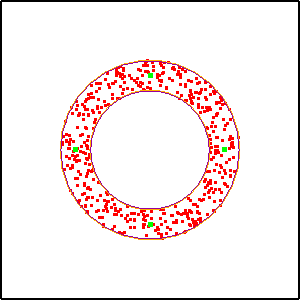
\includegraphics[height=5 cm]{figures/image62}
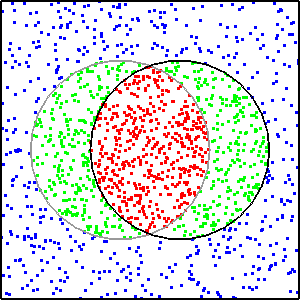
\includegraphics[height=5 cm]{figures/image63}
\caption{Output from compart.txt and compartlogic.txt, showing behavior of compartments.}
\label{fig:compart}
\end{figure}

This figure shows examples of compartments. In the left panel, green dots are the interior-defining points and red molecules were added randomly to the compartment. In the right panel, each circle was defined as a compartment and then the red, green, and blue molecule regions were defined with logical combinations of the left and right compartments.
For logically combining compartments, the logical options are: ``equal'', ``equalnot'', ``and'', ``andnot'', ``or'', ``ornot'', or ``xor''. These obey the standard logical rules. Note that the sequence of statements matters. For example, the region defined by A-andnot-B is the portion of A is that is not within B, whereas B-andnot-A is the portion of B that is not within A.

\section{Compartments and efficiency}

To test whether a given point is within a given compartment, Smoldyn starts by computing a line between that point and one of the interior-defining points. Smoldyn then tests whether this line crossed any of the panels of any of the compartment's bounding surfaces. If so, Smoldyn moves on to the next interior-defining point and repeats. The procedure stops as soon as a line can be drawn without crossing any surface panel, if that happens. This procedure is rapid for compartments with one panel and one interior-defining point, but can become extremely slow for surfaces with many panels and/or many interior-defining points. As a result, it is helpful to design compartments for efficient simulation. Also, it's best to avoid compartments if they aren't needed. For example, don't use the \ttt{reaction\_compartment} statement if you don't actually need the compartment testing.

\section{Statements about compartments}

The following table summarizes the statements about compartments.

\begin{longtable}[c]{ll}
Statement\\
\hline \\
\ttt{max\_compartment} $int$ & (optional statement)\\
\ttt{start\_compartment} $name$\\
\ttt{surface} $surface$\\
\ttt{point} $pos_0\ ...\ pos_{dim-1}$\\
\ttt{compartment} $logic\ compart$\\
\ttt{end\_compartment}
\end{longtable}

% Simulation settings
\chapter{Simulation settings}

\section{Simulation settings basics}

Several statements define how the simulation should be run. There are defaults for each of these settings, so the user does not need to set them directly. However, they can be useful for optimizing simulation performance. These settings include the random number generator seed, virtual boxes that partition the simulation volume, and some settings for diffusion on surfaces.

The simulation volume is partitioned into an array of virtual boxes, each of which is the same size and shape. In addition, each box that is on the edge of the simulation volume actually extends out to infinity in that direction, such that every location in space, whether in the simulation volume or not, is in some virtual box. These boxes do not affect the performance of the simulation, except for allowing computational efficiencies that speed it up.

\section{Random number seed}

As a default, the random number generator seed is set to the time at which the simulation is started. This is virtually certain to yield a unique random number sequence each time the simulation is run, so no two simulations will be identical. However, it can also be useful to set the random number generator seed, which can be done with the \ttt{random\_seed} statement. This statement can also be used to set the random number seed to the current time.

Smoldyn uses the Mersenne Twister random number generator, which has become a standard generator for many applications because it is fast and very high quality. Because Smoldyn uses this method rather than built-in generators, Smoldyn simulations that are run with the same seed produce the same results, regardless of the operating system or computer.

\section{Virtual boxes}

The box sizes can be left undefined, in which case a default is used, or they can be defined with either the \ttt{molperbox} or \ttt{boxsize} statements. The former statement sets the box sizes so that the average number of molecules per box, at simulation initiation, is close to the requested number. Good numbers tend to be between 3 and 6, although more or fewer may be appropriate, depending on how the number of molecules in the simulation is likely to change over time (the default box size is computed for an average of 4 molecules per box). The \ttt{boxsize} statement requests the length of one side of a box, which should be in the same units that are used for the boundary statements. Either way, the boxes that are actually created are unlikely to exactly match the requested values, but are sized to be as close to cubical as possible (or square for a 2-D simulation) and to exactly fill the simulation volume.

Box sizes that are too large will cause slow simulations, but no errors. Warnings that say that there are a lot of molecules or surface panels in a box are suggestions that smaller boxes may make the simulation run faster, but do not need to be heeded. Box sizes that are too small may cause errors. Several warnings can be generated for this, including that the diffusive step lengths are larger than the box size, etc. However, the only warning that really matters is if box sizes are smaller than the largest bimolecular reaction binding radius. If this happens, some bimolecular reactions are likely to be ignored, which will lead to a too slow reaction rate. If simulation speed is important, it is a good idea to run a few trial simulations with different box sizes to see which one leads to the fastest simulations.

The \ttt{accuracy} statement sets which neighboring boxes are checked for potential bimolecular reactions. Consider the reaction A + B $\rightarrow$ C and suppose that A and B are within a binding radius of each other. This reaction will always be performed if A and B are in the same virtual box. If accuracy is set to at least 3, then it will also occur if A and B are in nearest-neighbor virtual boxes. If it is at least 7, then the reaction will happen if they are in nearest-neighbor boxes that are separated by periodic boundary conditions. And if it is 9 or 10, then all edge and corner boxes are checked for reactions, which means that no potential reactions are overlooked. Overall, increasing accuracy numbers lead to improved quantitative bimolecular reaction rates, along with substantially slower simulations. If qualitative simulations are wanted, then lower accuracy values are likely to be preferable.

\section{Surface-bound molecule settings}

Several settings affect simulation of surface-bound molecules, described here. The default settings are nearly always good, although they can be modified if desired.

Molecules that are bound to a surface are given locations that are extremely close to that surface. However, this position does not need to be exactly at the surface, and in fact it usually cannot be exactly at the surface due to round-off error. The tolerance for how far a surface-bound molecule is allowed to be away from the surface can be set with the epsilon statement.

When a surface-bound molecule diffuses off of one surface panel, it can sometimes diffuse onto the neighboring surface panel. It does so only if the neighboring panel is declared to be a neighbor, as described above in the surfaces section, and also the neighbor is within a distance that is set with the \ttt{neighbor\_dist} statement. This value is set to an extremely small value by default, just large enough to prevent round-off error, and generally should not need changing. In some cases, moving a molecule to a point that is exactly on a panel edge can cause problems with round-off errors, so it is actually moved just inside the edge by a distance that can be set by the margin statement. Again, this should not need changing.

\section{Statements for simulation settings}

The following table summarizes the statements for simulation settings.

\begin{longtable}[c]{ll}
Statement & Description\\
\hline \\
\ttt{random\_seed} $int$ & random number seed\\
\ttt{accuracy} $float$ & accuracy code, from 0 to 10\\
\ttt{molperbox} $float$ & target molecules per virtual box\\
\ttt{boxsize} $float$ & target size of virtual boxes\\
\ttt{epsilon} $float$ & for surface-bound molecules\\
\ttt{margin} $float$ & for diffusing surface-bound molecules\\
\ttt{neighbor\_dist} $float$ & for diffusing surface-bound molecules
\end{longtable}


% Ports
\chapter{Ports}

\section{Port basics}

Ports are data structures that are used for importing and exporting molecules between a Smoldyn simulation and another simulation. In particular, they are designed for the incorporation of Smoldyn into MOOSE, but they could also be used to connect multiple Smoldyn simulations or for other connections.

A port is essentially a surface and a buffer. Smoldyn molecules that hit the porting surface are removed from the Smoldyn simulation and are put into the buffer for export. Once exported, they are removed from the buffer. Also, molecules may be added to the Smoldyn simulation at the porting surface by other programs.

\section{Defining ports}

Using the standard format, port statements are given in blocks that start with \ttt{start\_port} and end with \ttt{end\_port}. A port name is declared after \ttt{start\_port}. The porting surface is specified with surface and the active face of that surface is specified with face.

Also, in the definition of the surface that is to be used for porting (the surface has to be defined first), one has to specify that the active face of the surface has action ``port''.

\section{Statements about ports}

The following table lists statements about ports.

\begin{longtable}[c]{l}
Statement\\
\hline \\
\ttt{start\_port} $name$\\
\ttt{surface} $surface$\\
\ttt{face} $face$\\
\ttt{end\_port}
\end{longtable}

\section{Porting rate}

Some care is required to make ports work accurately. In particular, a port behaves for a Smoldyn simulation as an absorbing surface. The absorption rate depends on the simulation time step and molecular rms step length, as I described in Andrews, Physical Biology, 2009.


% Rule-based modeling with BioNetGen
\chapter{Rule-based modeling with BioNetGen}

\section{Rule-based modeling basics}

In many biochemical systems, proteins bind together into multimeric complexes and/or can be modified with phosphates, methyls, or other moieties. Each possible complex or protein state needs to be treated as a distinct chemical species in Smoldyn, as in many other simulators. However, even a fairly small list of complexation or modification reactions can lead to a large number of distinct species, and even more reactions that interconvert these species, making it impractical to enumerate all of the species and reactions manually. The solution is rule-based modeling, in which the user specifies the protein subunits and their binding rules, and then the software generates the species and reaction lists.

Smoldyn offers two types of rule-based modeling. First, you can use wildcards, which are explained in the Molecules chapter. Wildcards are very convenient but not good for complicated reaction networks. Secondly, you can use Smoldyn's BioNetGen module, which uses the BioNetGen software. This software has been thoroughly validated and is widely used. BioNetGen generates the entire reaction network at once, as opposed to ``on-the-fly,'' in which the network is only expanded as needed.

To use BioNetGen rule-based modeling with Smoldyn, you need to write a rules file in the BioNetGen language, called BNGL, and save it as a plain text file but with a .bngl suffix. Once you have a rules file, you can either convert it to a reaction network yourself, using the BioNetGen BNG2.pl program (a perl script), or you can tell Smoldyn to convert it to a reaction network, which it does by calling the same BNG2.pl program. The former approach has the advantage of separating the steps more cleanly, which might be easier for debugging, understanding the output, or setting up multiple simulations more efficiently. The latter approach is a little more automated, which might be better for making the code simpler for yourself or other users. Either way, BNG2.pl saves the reaction network as a plain text file that has a .net suffix (which is fairly easy to understand). Then, Smoldyn reads in this reaction network, adding the generated species and reactions to its internal lists. During the process, Smoldyn also computes diffusion coefficients, default states, display colors, display sizes, and molecule-surface interactions for the new species, as explained below.

\section{Writing rules in BNGL}

The BNGL language is relatively simple to use for most models. The language also has many more sophisticated portions, for which interested readers should refer to the BioNetGen website and publications by the BioNetGen team; the most relevant publication, which is included in the documentation directory of the download package, is ``Rule-Based Modeling of Biochemical Systems with BioNetGen'' by Faeder, Blinov, and Hlavacek, Methods in Molecular Biology, Systems Biology 500:113, 2009.

The following example file is called abba.bngl, named for the structure of the complete complex (A-B-B-A).

\begin{lstlisting}[style=SSAC]
# BioNetGen file, run in Smoldyn with abbasim.txt

setOption("SpeciesLabel","HNauty")

begin model
begin parameters
	Anumber   100
	Bnumber   100
	kab_on	200
	kab_off	2
	kbb_on	80
	kbb_off	1
end parameters

begin seed species
	A(a2b)		Anumber
	B(b2a,b2b)	Bnumber
end seed species

begin reaction rules
	# A bind to B
	A(a2b) + B(b2a) <-> A(a2b!1).B(b2a!1) kab_on,kab_off
	# B bind to B
	B(b2b) + B(b2b) <-> B(b2b!1).B(b2b!1) kbb_on,kbb_off
end reaction rules
end model

## actions ##
generate_network({overwrite=>1})
\end{lstlisting}

The \ttt{setOption} statement tells BioNetGen how to do graph isomorphism checking. The HNauty method, used here, is always a good approach. The model definition portion of the file, which is essentially the entire file, starts with begin model and ends with end model statements. Within this are three blocks: ``parameters'' in which you can define the values of variables, ``seed species'' in which you define the monomers of the multimeric complexes and how many the simulation should start with, and ``reaction rules'' in which you define the rules for the possible complexation reactions, along with their reaction rates. Each block begins with a begin statement and ends with an end statement.

The parameters block defines parameters and lists their values. In the seed species definitions, each line lists one subunit and all of its binding sites. Here, the A species has only one binding site, called a2b and the B species has two binding sites, called b2a and b2b. These species are followed by the number of molecules to include in the simulation (which will be randomly placed within the simulation volume). Although not done here, it is typically easiest to set these molecule counts to 0 and to then add monomers to the simulation with mol, \ttt{surface\_mol}, or \ttt{compartment\_mol} statements in the Smoldyn input file. The reaction rules describe how things can bind together. In the first rule, for example, A can bind to B using the a2b site on A molecules and the b2a site on B molecules. The b2b site of B molecules does not affect this binding, so it is ignored in the rule (alternatively, this rule could have specified that the b2b site must be bound, or unbound, for this reaction to occur). On the right hand side of the rule, the period between the species indicates a bond and the ``!1'' text labels the bond number; this latter notation is useful for distinguishing bonds when there are multiple bonds in a single rule. Finally, the reaction rate is followed by forward and reverse reaction rate constants. The last line of the file tells BioNetGen to generate the network and to overwrite any previous output file. Note that BioNetGen can also do quite a lot of other things in addition to simply generating the network, including running non-spatial simulations; see the BioNetGen documentation for these.

\section{Writing the Smoldyn file to read the rules or generated network}

The following Smoldyn file reads and simulates the abba network.

\begin{lstlisting}[style=SSAC]
# Smoldyn configuration file to run abba.bngl BioNetGen network.

# Graphical output
graphics opengl_good

# System space and time definitions
dim 2
boundaries x 0 100 p
boundaries y 0 100 p
time_start 0
time_stop 1000
time_step 0.01

# Molecular species and their properties
species A B
difc A 3
difc B 1
color A green
color B red
display_size all(all) 2

start_bng abba
multiply unimolecular_rate 1
multiply bimolecular_rate 1
#BNG2_path ../../../source/BioNetGen/BNG2.pl
expand_rules abba.bngl
read_file abba.net
end_bng

text_display time A B A.1.B.1.0 B.2.0 A.1.B.2.0 A.2.B.2.0

end_file
\end{lstlisting}

This file declares the A and B species with a species statement and then gives their diffusion coefficients and graphical display parameters. Later on, while parsing the BioNetGen output, Smoldyn will assign these same values to the A and B monomers.

The BioNetGen portion of this file is in the ``bng'' block. It starts with the \ttt{start\_bng} statement and the network name (you can also name the block using the name statement) and ends with \ttt{end\_bng}. Within this block, Smoldyn recognizes some statements that are specific to Smoldyn, as well as text from the BioNetGen .net file (i.e. you can just copy and paste the .net file into here if you like). The \ttt{multiply} statements shown here enable you to enter factors with which Smoldyn will multiply the unimolecular or bimolecular reaction rates. This is useful to make unit conversions in case you used different units for reaction rates in the rules file and in the rest of the Smoldyn configuration file. The \ttt{BNG2\_path} statement, which is commented out here, specifies the directory path to the BNG2.pl software. Ideally, the default path (set to /usr/local/bin for Macs and Linux), will be correct and you won't need to specify it here. However, if the default does not work correctly, then you can give it here instead. The \ttt{expand\_rules} statement, with the filename of the rules file, tells Smoldyn to call BNG2.pl, which will then expand the reaction network and save the result as a .net file; Smoldyn does not parse the results at this point. Finally, \ttt{read\_file} is a standard Smoldyn statement, which in this case reads in the .net file, adding the species and reactions to the simulation in the process. The last line of this file tells Smoldyn to display the species counts to the display.

When you run this configuration file in Smoldyn, you should, as always, look at Smoldyn's diagnostic text output. In this case, the BioNetGen portion of the output includes the following:

\begin{lstlisting}[style=SSAC]
 species allocated: 7, defined: 7
   1 A (solution), count: 100, longname: A(a2b)
   2 B (solution), count: 100, longname: B(b2a,b2b)
   3 A.1.B.1.0 (solution), count: 0, longname: A(a2b!1).B(b2a!1,b2b)
   4 B.2.0 (solution), count: 0, longname: B(b2a,b2b!1).B(b2a,b2b!1)
   5 A.1.B.2.0 (solution), count: 0, longname:
						A(a2b!1).B(b2a!1,b2b!2).B(b2a,b2b!2)
   6 A.2.B.2.0 (solution), count: 0, longname:
						A(a2b!1).A(a2b!2).B(b2a!2,b2b!3).B(b2a!1,b2b!3)
  reactions allocated: 15, defined: 13
   1 A + B -> A.1.B.1.0  rate: 200
   2 B + B -> B.2.0  rate: 80
   3 A + B.2.0 -> A.1.B.2.0  rate: 400
   4 A.1.B.1.0 -> A + B  rate: 2
   5 B + A.1.B.1.0 -> A.1.B.2.0  rate: 80
   6 A.1.B.1.0 + A.1.B.1.0 -> A.2.B.2.0  rate: 80
   7 B.2.0 -> B + B  rate: 1
   8 A + A.1.B.2.0 -> A.2.B.2.0  rate: 200
   9 A.1.B.2.0 -> A + B.2.0  rate: 2
   10 A.2.B.2.0 -> A + A.1.B.2.0  rate: 4
   11 A.1.B.2.0 -> B + A.1.B.1.0  rate: 1
   12 A.2.B.2.0 -> A.1.B.1.0 + A.1.B.1.0  rate: 1
\end{lstlisting}

The species list shows that each species has both a short name and a long name. The long names were generated by BioNetGen and give the full binding information. The short names were shortened by Smoldyn for more convenient use. They list only the numbers of each monomer type in a species, followed by an ``isomer index'' in case there are multiple complexes with the same stoichiometry. The reaction list is shown using the short names. Note that the reaction rates account correctly for the species' binding sites; for example, reaction 3 has rate 400, rather than the value of 200 that was given in the rules file for A-B binding, due to the fact that the A molecule in this reaction can bind to either of two B monomers.

\section{Creating species groups in BioNetGen}

It is often helpful to be able to output not just the number of a molecules of individual species, but the number of molecules of all species that share some specific property. For example, one might want the total number of molecules that include at least one AB group, independent of what else is bound to them. To do so, you can define a species group using an ``observables'' section in the BNGL file. These observables become species groups in the main Smoldyn program, as described above the in the Molecules chapter. Each observable needs to have a name and then a species pattern that tells which species are included. For example, adding these lines to the ABBA.bngl file would create a species group called ABgroup:

\begin{lstlisting}[style=SSAC]
begin observables
  Species ABgroup A(a2b!1).B(b2a!1)
end observables
\end{lstlisting}

Species groups defined in this way can be used in most Smoldyn statements and commands.

\section{Statements for rule-based modeling}

The following list summarizes the statements for rule-based modeling.

\begin{longtable}[c]{l}
Statement\\
\hline\\
\ttt{start\_bng} $name$\\
\ttt{end\_bng}\\
\ttt{name} $name$\\
\ttt{multiply unimolecular\_rate} $value$\\
\ttt{multiply bimolecular\_rate} $value$\\
\ttt{monomer\_state} $monomer\ state$\\
\ttt{BNG2\_path} $path$\\
\ttt{bng\_file} $filename$
\end{longtable}

\section{A ligand-receptor-messenger system in BioNetGen}

The following BioNetGen and Smoldyn files represent a ligand-receptor-messenger signaling system. In it, both an extracellular ligand and an intracellular messenger protein can bind to opposite sides of a trans-membrane receptor. When a receptor binds both at once, it causes the messenger to become phosphorylated, thus transmitting the ligand-binding event to an intracellular signal. The messenger protein dephosphorylates spontaneously. This is substantially more complicated than the above ABBA simulation because it uses monomer modification sites and surface-bound molecules. The following sections discuss these files.

\begin{lstlisting}[style=SSAC]
# BNGL file, saved as lrm.bngl.
# BioNetGen file, run in Smoldyn with surfacestatessim.txt

setOption("SpeciesLabel","HNauty")

begin model
begin parameters
	krl_on	20
	krl_off	0.01
	krm_on	10
	krm_off	0.02
	k_phos	2
	k_unphos 2
end parameters

begin molecule types
	L(l2r)
	R(r2l,r2m)
	M(m2r,psite~u~p)
end molecule types

begin seed species
	L(l2r)		0
	R(r2l,r2m)	0
	M(m2r,psite~u)	0
end seed species

begin reaction rules
	L(l2r) + R(r2l) <-> L(l2r!1).R(r2l!1)	krl_on,krl_off
	R(r2m) + M(m2r) <-> R(r2m!1).M(m2r!1)	krm_on,krm_off
	R(r2l!+,r2m!1).M(m2r!1,psite~u) -> R(r2l!+,r2m!1).M(m2r!1,psite~p)
								k_phos
	M(psite~p) -> M(psite~u)	k_unphos
end reaction rules

begin observables
	Species Rbound R(r2l!+)
end observables
end model

## actions ##
generate_network({overwrite=>1})
\end{lstlisting}

Following is another Smoldyn file, saved as lrmsim.txt:

\begin{lstlisting}[style=SSAC]
#Smoldyn file, saved as lrmsim.txt
# Smoldyn configuration file to run abba.bngl BioNetGen network.

# Graphical output
graphics opengl_good

# System space and time definitions
dim 2
boundaries x 0 100
boundaries y 0 100
time_start 0
time_stop 1000
time_step 0.05

# Molecular species and their properties
species L R M.1.0 M.1.1
difc L 3
difc R(up) 0.2
difc M.1.0 2
difc M.1.1 1.5
color L(all) green
color R(all) blue
color M.1.0(all) orange
color M.1.1(all) red
display_size all(all) 2

# BioNetGen parameters
start_bng lrm
multiply unimolecular_rate 1
multiply bimolecular_rate 1
#BNG2_path ../../../source/BioNetGen/BNG2.pl
monomer_state L fsoln
monomer_state R up
monomer_state M bsoln
expand_rules lrm.bngl
read_file lrm.net
end_bng

# Surface parameters
start_surface membrane
action both all(all) reflect
panel rect +1 0 50 100
end_surface

start_surface outsides
action both all(all) reflect
panel rect +x 0 0 100
panel rect -x 100 0 100
panel rect +y 0 0 100
panel rect -y 0 100 100
end_surface

# initial molecules
surface_mol 20 R(up) membrane all all
mol 20 L 50 80
mol 20 M.1.0 50 20

end_file
\end{lstlisting}

\section{Network expansion with monomer modifications}

Monomers can have modification sites, such as sites that can accept phosphate or methyl groups. Using these modification sites can be preferable to treating them as complexation reactions with phosphate or methyl molecules because doing so avoids needing to treat the additional molecules explicitly.

Enter modification sites in the BNGL language by defining the monomers in a ``molecule types'' block. This block is optional when not using modification sites. In this block, list the different monomers, along with their binding sites. List modification sites similarly to binding sites, but follow the site name with a sequence of tildes and the possible modifications. In the lrm example, \ttt{M(m2r,psite$\sim$u$\sim$p)} declares the monomer M, which has a binding site called m2r and a modification site called psite. This modification site can adopt either the ``u'' or the ``p'' condition. In this case, the seed species block specifies that network expansion should start with unphosphorylated M using \ttt{M(m2r,psite$\sim$u)}, but does not include phosphorylated M.

The molecule types and seed species blocks appear to be essentially the same, but aren't actually. The molecule types block is used to define each of the monomers, including all of their binding sites and modification sites. The seed species block includes a list of species (which are typically, but not necessarily monomeric). When expanding the reaction network, BioNetGen starts with each of these seed species, finds their reactions and reaction products, then finds the reactions and products of the newly generated species, and so on, eventually generating the entire reaction network. If a portion of the network cannot be reached from the given list of seed species, then BioNetGen does not generate it. Nevertheless, there is high overlap between the two blocks, which is why the molecule types block is optional when there are no modification sites.
Note the use of modification sites in the reaction rules. Also, the third reaction rule has the reactant \ttt{R(r2l!+,r2m!1).M(m2r!1,psite$\sim$u)}. The notation !+ indicates that the r2l site needs to be bound to something, but does not specify the binding partner.

Smoldyn interprets modification sites as creating different isomers of a species. For this reason, there is no species called just M in this simulation, because it would be unclear which modification state that would represent. Instead, the two species are M.1.0 and M.1.1, where the former 1 denotes that there is 1 M monomer and the latter 0 or 1 denotes the isomer number (which, in this case, corresponds to the ``u'' and the ``p'' condition, respectively). This Smoldyn file defines the diffusion coefficient, color, and display size for both M isomers, which are then used in the simulation. If the file did not define them, Smoldyn would have looked for these attributes for a species named M or one called M.$x$.$y$, where $x$ and $y$ are any numbers, and used those instead.

\section{Network expansion with surface-bound states}

The lrm simulation also uses surface-bound states. These do not appear in the BioNetGen file at all. Instead, they show up in the Smoldyn file in a couple of places. First, trivially, they are used in the diffusion coefficient and graphical display statements, where they ensure that the attributes get assigned to the correct states of the species. They also appear in the bng block, in the \ttt{monomer\_state} statement. This specifies the state (solution, ``bsoln,'' or a surface-bound state) in which each monomer is typically found. Smoldyn uses these to infer states for reaction products.

For example, this file says that ligands are in fsoln state, receptors in the up state, and messenger proteins in the bsoln state. From these, Smoldyn assigns states to some of the reactions as:

\begin{lstlisting}[style=SSAC]
L + R (up) -> L.1.R.1.0 (up)
L.1.R.1.0 (up) -> L + R (up)

R (up) + M.1.0 (bsoln) -> M.1.R.1.0 (up)
M.1.R.1.0 (up) -> R (up) + M.1.0 (bsoln)
\end{lstlisting}

Smoldyn uses the method that the state for a species is the highest precedence of the states for the species' subunits. In the first reaction, for example, the species L.1.R.1.0 has an L monomer with state fsoln and an R monomer with state up, and the up state takes precedence, so the species is assigned state up. The precedence order is: solution, ``bsoln,'' and then surface-bound states in the order front, back, up, and down.

\section{Short names, diffusion coefficients, and graphical parameters}

Smoldyn assigns short names to each species that BioNetGen generates. As mentioned briefly above, the format is that it lists each monomer and the number of copies of that monomer in the species, and then an isomer number at the end, with the items separated by periods. Smoldyn gets the monomer names from the species' long names, which BioNetGen generates. The monomers are listed in alphabetical order. If a species has only a single monomer in it and there are no modification sites for this monomer, then Smoldyn abbreviates the short name to just the same name as the monomer. Note that a monomer and a species that has just a single monomer can have the same names and are chemically identical, but are conceptually different in the software; one is a monomer, which only exists in the context of parsing BioNetGen files, and the other is a species, which is part of a Smoldyn simulation. Smoldyn assigns isomer numbers based on the order in which it encounters the species in the BioNetGen output file. Thus, there is no a priori way to know what the isomer number will be. The best approach is to figure out which is which by reading the long name portion of the bng output.

For each monomer, Smoldyn looks for information with which it can assign diffusion coefficients and graphical parameters. First, it sees whether the user assigned these using \ttt{monomer\_difc}, \ttt{monomer\_color}, or \ttt{monomer\_display\_size} statements (very similar to the \ttt{monomer\_state} statement). If not, Smoldyn sees whether the user created a species that has the same name as the monomer, and then uses its attributes. If this fails, then Smoldyn sees whether there is a species that has the monomer name followed by a .$x$.$y$ suffix, where $x$ and $y$ are additional text, and uses its attributes. If all of these fail, then Smoldyn simply assigns the monomer diffusion coefficient to 0, the color to black, and the display size to 0.

For species, Smoldyn again starts by looking for definitions given in the input file. If none were given, then it computes diffusion coefficients and graphics parameters based upon the values for the monomers that compose the species. In doing so, it assumes that the mass of a species is the sum of the monomer masses and also that both monomers and complexes of monomers are roughly spherical and have similar densities. From these assumptions, the radius of a complex is the cube root of the sum of the cubes of the monomer radii. Based on this, Smoldyn assigns a species display size as
$$S_{species} = \left( \sum_i S_i^3 \right)^{\frac{1}{3}}$$
where $S_i$ is the display size of the $i$'th monomer. Smoldyn also assumes that the diffusion coefficient scales as the inverse of the species radius, from the Stokes-Einstein equation. From this, it computes the diffusion coefficient for a complex using
$$D_{species} = \left( \sum_i D_i^{-3} \right)^{-\frac{1}{3}}$$
where $D_i$ is the diffusion coefficient of the $i$'th monomer. Smoldyn computes colors for species by computing the arithmetic average of the red, green, and blue color values for each of the monomers.

\section{Surface-molecule interactions}

If your block of BioNetGen statements comes before your surface definitions in your Smoldyn input file, then all of the species will have been generated before Smoldyn starts defining surfaces. In this case, you can set surface actions or rates for the newly generated species yourself. In the surface action or rate statements, you can list these species individually, all at once using the ``all'' option, or selectively using species groups or wildcards.

The other option is to define surfaces before expanding the reaction network with BioNetGen. In this case, Smoldyn infers the molecule-surface interactions for the newly generated species, much as Smoldyn computes diffusion coefficients, colors, and display sizes for them. As for those other species properties, Smoldyn considers the monomers that compose the new species and looks at the molecule-surface interactions for those monomeric species. The surface action for a multimeric complex is that of the component monomer that has the greatest action. In order of increasing action, the possibilities are: transmit, multiple actions, reflect, jump, absorb, and port. Multiple actions mean that there is some rate, such as for adsorption or desorption. If Smoldyn needs to choose between two monomers with multiple actions, then Smoldyn chooses the one with the faster rate constant. The polymer\_endsim.txt file illustrates this, although in a fairly minimal manner.


% Filaments
\chapter{Filaments}

\section{Status}

I am working on adding simulation support for filaments to Smoldyn, but have only just begun. At present, it is possible to define filaments and specify their geometries by adding monomers to them. These filaments can move by treadmilling, and they interact with surfaces. They do not exhibit Brownian motion. See the examples in the S13\_filaments directory.


% Hybrid simulation
\chapter{Hybrid simulation}

Most of the Smoldyn software is developed around the Smoluchowski level of detail. Here, each individual molecule of interest in the simulation is represented as a small sphere that has a precisely defined position in continuous space. This offers spatial accuracy down to nanometer size scales for typical systems, which is more detailed than that offered by most other comparable simulation software, but is necessary when studying biophysical processes that take place on these spatial scales. The cost of this high level of detail is that simulations become computationally demanding, both in terms of the number of processes that have to be run at each simulation time step and in terms of the memory required to store all of the molecular information. Hybrid simulations can offer solutions for simulating models with both high levels of detail and high speed, which they accomplish by representing high levels of detail only as needed.

The hybrid methods that are particularly important here combine particle-based simulation with lattice-based simulation. The particle-based simulation methods are Smoldyn's standard methods, which work at the Smoluchowski level of detail. The lattice-based methods represent spatially compartmentalized versions of the chemical master equation, typically simulated using one of the spatial Gillespie methods (partial differential equations or spatial Langevin methods are also appropriate). Hybrid methods can use either overlapping space or adjacent space methods. In the former case, the physical space represented by the lattice-based methods is the same as that by the particle-based methods; molecules in one representation can interact with spatially proximate molecules that are in the other representation. Smoldyn has been added to Virtual Cell in this manner, where VCell provides the lattice representation and Smoldyn provides the particle representation. Here, the lattice representation is best for abundant or rapidly diffusing species where exact molecule positions don't matter, and the particle representation for rare species where the extra computational effort is necessary. In the latter case, the particle-based and lattice-based methods represent adjacent regions of physical space. Molecules can diffuse back and forth between the two regions, changing representations as they do so. This approach is best in cases where one region of space needs to be simulated in detail, while surrounding regions can be simulated more coarsely. The remainder of this section focuses on this latter adjacent space approach.

\section{Hybrid simulation basics}

The lattice module incorporated into Smoldyn is fairly simple. It represents lattices using an axis-aligned rectangular array of subvolumes. It simulates chemical reactions using the next subvolume (NSV) method, which treats molecules as discrete objects (i.e. not continuously variable concentrations) and captures reaction stochasticity accurately. Whereas simulation time advances with fixed length time steps in the particle-based methods, it advances with unequal steps, from event to event, in the NSV method. The lattice region of space can be bounded by a few different boundary types, but the lattice code does not currently address interactions between molecules and any surfaces that are within the lattice region of space. The junction between the particle-based region of space and the lattice region of space is created using a Smoldyn ``port'', explained above.

\section{Defining lattices}

To include a lattice in a model, you need to add a lattice, obviously. This is entered using a block of statements that starts with \ttt{start\_lattice} and ends with \ttt{end\_lattice}, much like similar blocks for surfaces, compartments, and other things. The definitions that can be entered within this block are discussed below. In addition to adding a lattice, you also need to define a port, which will form the junction between the particle space and the lattice space. And to create a port, you will need to define at least one surface. The examples/S14\_lattices/diffusion.txt file shows a very simple example of model that uses a lattice.

First, it's a good idea to define the lattice type using the type statement. In principle, this will enable you to choose whether the lattice region is simulated with discrete numbers of molecules using NSV algorithm, with continuous concentrations using PDE algorithms, or with other methods. In practice though, only NSV is currently implemented, and NSV is the default, so you don't actually need to define the type. On the other hand, you do need to define the port that separates particle space from lattice space, using the port statement.
Define the boundaries of the lattice space using the boundaries statement. It is essentially identical to the boundaries statement for the main portion of the configuration file, but that one only applies to the particle region of space and this one only applies to the lattice region of space. The two sets of boundaries are typically strictly adjacent to each other, with no gap and no overlap, but it is also just fine if they overlap. The port should obviously be at the intersection of the two sets of boundaries, or somewhere within the overlap region. By default, the lattice boundaries are reflective, but they can also be periodic. These are entered with optional characters after the rest of the statement, exactly as for the particle side boundaries statement.

Lattice partitioning is defined using the \ttt{lengthscale} statement. The values entered here should be even divisors of the \ttt{boundaries} dimensions. Also, make sure that the port is at a partition boundary and make sure that there is at least one partition on either side of the port. Note that misalignments can arise from round-off errors. To avoid this, use boundaries, port positions, and lattice compartment sizes that are integers, or that use an integer power of two decimal (e.g. 0.5, 0.25, 0.375, etc., but not 0.1, 0.2, 0.3, etc.).

Use the \ttt{species} and \ttt{reactions} statements to tell a lattice which species and reactions it should work with. Often, ``all'' is used, meaning that the lattice should know about all of the same species and/or reactions as the particle side of the simulation uses. However, it's also possible to specify a subset of the total species and reactions lists. This is useful because the lattice code runtime increases with more species and with more reactions, unlike the particle side, which increases with numbers of individual molecules. Lattices cannot work with any species or reactions that are not also defined in the particle side. However, it is possible to have a reaction only perform on the lattice side. In this case, define the reaction on the particle side, with a rate constant as usual. Then, when listing the reactions that the lattice side should work with, use the keyword ``move'' to indicate that all subsequent reactions in the list should be ``moved'' to the lattice side and disabled on the particle side.

Finally, use the \ttt{mol} statement to add molecules to the lattice side. This is essentially identical to the statement of the same name in the main portion of the configuration file, but only applies to the lattice side of space.

\section{Lattice output}

Several commands output information from lattices. \ttt{printLattice} outputs some basic information about the lattice, including the low and high corners of the lattice space, the subvolume partition spacing, and the total number of each species in the lattice. This is the same output that is displayed with the simulation diagnostics.

\ttt{molcount} and \ttt{molcountspace} are functions that are often used with non-lattice simulations. In addition to counting molecules in the particle region of space, they also count molecules in the lattice region; there is no way to select just particle region or just lattice region. \ttt{molcountspace} does not count molecules that are in transit between representations (if you select a single species and state; it does if you select all species and/or all states), so it will miss a few molecules. \ttt{savesim} saves the full simulation state; it saves the lattice state as well as the rest. Other molecule counting commands do not include lattice molecules.

Finally, \ttt{writeVTK} produces VTK output for both the particle and lattice regions of space. It does not include surface information. The output is saved as a stack of files that have names that follow the format $filename$Lattice00\_00001.vtu and $filename$Molecules00001.vtu, and that have incremented numbers for subsequent snapshots. This output can be viewed using Paraview, Visit, or other VTK viewers. It doesn't appear that any of them are trivial to use.

\section{Statements about lattices}

The following table summarizes the statements about lattices.

\begin{longtable}[c]{ll}
Statement & Description\\
\ttt{start\_lattice} $name$ & start defining a lattice\\
\ttt{type} $type$ & type of the lattice (``nsv'')\\
\ttt{port} $port$ & port for exchanging molecules\\
\ttt{boundaries} $dim\ pos_1\ pos_2\ type$ & boundaries of the lattice region of space\\
\ttt{lengthscale} $x_1\ x_2\ x_3$ & partition spacing for lattice subvolumes\\
\ttt{species} $species_1\ species_2\ ...$ & species that the lattice should recognize\\
\ttt{reaction} $[move]\ reaction_1\ reaction_2\ ...$ & reactions that the lattice should recognize\\
\ttt{mol} $nmol\ name\ pos_0\ pos_1\ �\ pos_{dim-1}$ & starting molecules in the lattice space\\
\ttt{end\_lattice} & end the lattice block
\end{longtable}


% Python and C/C++ interfaces
\chapter{Python and C/C++ interfaces}

Libsmoldyn is a C, C++, and Python interface to the Smoldyn simulator. It complements the stand-alone Smoldyn program in that it is a little more difficult to use, but it provides much more flexibility. Libsmoldyn provides: (1) an application programming interface (API) that will be relatively stable, even as Smoldyn is updated and improved, (2) function names that are relatively sensible and that shouldn't collide with other function names in other software, and (3) reasonably thorough error checking in every function which helps ensure that the user is using the function in a sensible way and in a way that won't crash Smoldyn. Libsmoldyn was originally written as a C API, but should work with C++ as well. It also offers Python bindings, which are still quite new but generally work well and are more convenient for most applications.

\section{Installing}

It's best to install Smoldyn twice. First, download the latest package from \url{http://www.smoldyn.org} and run the install script. This will install the stand-alone program, the C/C++ libraries, and the BioNetGen code, and will also give you the documentation and example files.

Next, install the Python components from PyPI with:
\begin{lstlisting}[style=SSAC]
pip install smoldyn
\end{lstlisting}
If this doesn't work, then a different possibility is:
\begin{lstlisting}[style=SSAC]
python3 -m pip install smoldyn --user --pre
\end{lstlisting}
Either of these should install the smoldyn nightly package, from: \url{https://pypi.org/project/smoldyn/}. For Windows, Python is often called ``py'', so try this if the above doesn't work (or your computer asks you to download Python from the Windows store, which probably isn't necessary). For those who are curious, the ``-m'' option means to run pip as a python module, the ``--user'' option means to install to the user directory, and the ``--pre'' option means to include pre-release versions. Feel free to try more or fewer options, of course. Also, some other useful pip options are: ``pip uninstall smoldyn'', ``pip cache purge'' (pip installs from its cached version if it already has one, so this is useful if you want to force it to download the online version), and ``pip search smoldyn''.

Alternatively, the Mac distribution, downloaded from \url{http://www.smoldyn.org/downloads/} comes with a Python wheel, called something like smoldyn-2.62-py3-none-any.whl. After installing with the software with the ``install.sh'' script, you should be able to write ``pip install smoldyn...whl'' and that will install it for you as well.

After installing, it might just run. If not, then the next challenge is to get your system to know that it's allowed to run the files. There are a few ways to do this. (1) You can navigate to one directory above where the ``\_\_init\_\_.py'' file gets stored and work from there. To try this out, go there and start Python; then try \ttt{import smoldyn} and see if it works. (2) You can set \ttt{PYTHONPATH} environment variable to the install location. However, this only works for the current command-line session and needs to be reset for the next one. To see its current value, for Mac or Linux, enter \ttt{echo \$PYTHONPATH}. (3) You can modify your sys.path variable to include a path to the install location, which then lasts for new command-line sessions as well. To see its current value, start Python and enter: \ttt{import sys; print(sys.path)}.

\section{Current limitations}

The Python interface has a few limitations that users should be aware of. We are working on fixing them.

\begin{itemize}

\item{Rule-based modeling}. Rule-based modeling support, including both BioNetGen and Smoldyn wildcards, has not been added to Libsmoldyn yet, including its Python API.

\textbf{Hybrid simulation}. Smoldyn has built-in support for multiscale simulation in which part of the model volume is simulated with particle-based methods and part with spatial Gillespie methods. These parts are typically adjacent to each other but can also overlap. This functionality has not been added to Libsmoldyn yet, including its Python API.

\item{Python quits after simulation if graphics are used}. A benefit of running Smoldyn through the Python interface is that the simulation and data analysis code can be included in the same Python file. Unfortunately, the OpenGL glut library that Smoldyn uses to display its graphical output does not return control to Smoldyn after the user quits the graphics but returns to the operating system, making it impossible to continue with further Python code. The only good solution for now is to display graphics while developing a simulation, and then re-run simulations with graphics turned off when collecting quantitative data. Note that the random number seed can be set to the same value in each case so that the simulation will be exactly the same.

\textbf{TIFF output doesn't work on some computers.} For some reason, Smoldyn cannot output TIFF files when run through the Python interface, at least on some computers. The Smoldyn code itself runs just fine, but it calls the \ttt{TIFFOpen} function in the libtiff library, which somehow refuses to open a new TIFF file. Alternative options for exporting graphics are: (1) rewrite the model without the Python interface, (2) save the current model and state using the savesim command, and then run that using the stand-alone Smoldyn software (i.e. the Smoldyn application, without the Python interface), (3) pause the simulation and capture the graphics using a screen grab, (4) use the VTK graphical output option. Yet another option is to convince a Smoldyn developer to add png export support for Smoldyn, such as with the ``Tiny PNG Output'' project, which looks fairly easy but hasn't been done yet.

\end{itemize}

% Python API example
\section{Python API example}

The following example, template.py, is from the ``examples'' directory in the Smoldyn download. It simulates a Michaelis-Menten reaction in which substrates and products diffuse freely within a circular membrane (it's simulated in two dimensions, for simplicity) and enzymes are bound to the membrane.

\begin{lstlisting}[style=SSAPython]
1   """Template for writing Smoldyn model in Python
2   
3   Use standard docstring to list basic file information here, including your
4   name, the development date, what this file does, the model name if you want
5   one, units used, the file version, distribution terms, etc.
6   
7   Enzymatic reactions on a surface, by Steve Andrews, October 2009. Modified by
8   Dilawar Singh, 2020. This model is in the public domain. Units are microns and seconds.
9   The model was published in Andrews (2012) Methods for Molecular Biology, 804:519.
10  It executes a Michaelis-Menten reaction within and on the surface of a 2D circle.
11  """
12   
13  __author__ = "Dilawar Singh"
14  __email__ = "dilawars@ncbs.res.in"
15  
16  import smoldyn 
17  
18  # Model parameters
19  K_FWD = 0.001    # substrate-enzyme association reaction rate
20  K_BACK = 1       # complex dissociation reaction rate
21  K_PROD = 1       # complex reaction rate to product
22   
23  # Simulation starts with declaring a Simulation object with the system boundaries.
24  s = smoldyn.Simulation(low=[-1, -1], high=[1, 1])
25  
26  # Molecular species and their properties
27  # Species: S=substrate, E=enzyme, ES=complex, P=product
28  # Type `help(smoldyn.Species)` in Python console to see all parameters.
29  S = s.addSpecies("S", difc=3, color=dict(all="green"), display_size=dict(all=0.02))
30  E = s.addSpecies("E", color=dict(all="darkred"), display_size=dict(all=0.03))
31  P = s.addSpecies("P", difc=3, color=dict(all="darkblue"), display_size=dict(all=0.02))
32  ES = s.addSpecies("ES", color=dict(all="orange"), display_size=dict(all=0.03))
33  
34  # Surfaces in and their properties. Each surface requires at least one panel.
35  # Add action to `both` faces for surface. You can also use `front` or `back`
36  # as well. Here, `all` molecules reflect at both surface faces.
37  sph1 = smoldyn.Sphere(center=(0, 0), radius=1, slices=50)
38  membrane = s.addSurface("membrane", panels=[sph1])
39  membrane.setAction('both', [S, E, P, ES], "reflect")
40  membrane.setStyle('both', color="black", thickness=1)
41  
42  # Define a compartment, which is region inside the 'membrane' surface.
43  inside = s.addCompartment(name="inside", surface=membrane, point=[0, 0])
44  
45  # Chemical reactions. Here, E + S <-> ES -> P
46  r1 = s.addBidirectionalReaction(
47      "r1", subs=[(E,"front"), (S,"bsoln")], prds=[(ES,"front")], kf=K_FWD, kb=K_BACK)
48  r1.reverse.productPlacement("pgemmax", 0.2)
49  
50  r2 = s.addReaction(
51      "r2", subs=[(ES, "front")], prds=[(E, "front"), (P, "bsoln")], rate=K_PROD)
52  
53  # Place molecules for initial condition
54  inside.addMolecules(S, 500)
55  membrane.addMolecules((E, "front"), 100)
56  
57  # Output and other run-time commands
58  s.setOutputFile('templateout.txt', True)
59  s.addCommand(cmd="molcountheader templateout.txt", cmd_type="B")
60  s.addCommand(cmd="molcount templateout.txt", cmd_type="N", step=10)
61  
62  s.setGraphics(
63      "opengl_good", bg_color="white", frame_thickness=1,
64      text_display=["time", S, (E, "front"), (ES, "front"), P] )
65  s = s.run(stop=10, dt=0.01)
\end{lstlisting}

\begin{description}

\item{1-11.} The file starts with a docstring, which is a useful way to provide information about the model, authors, etc. Smoldyn does not handle units at all, so it's the user's responsibility to make sure that all units are consistent with each other. The best approach is simply to make sure that all lengths use the same units, such as nanometers or microns, and all times use the same units, such as milliseconds. This also applies to derived units, such as volumes and rate constants.

\item{13-14.} Entering the author and email address with double underscores follows good Python form.

\item{16.} Import the Smoldyn Python API with ``import smoldyn''. If you want the low-level Python API, then import it with ``import smoldyn.\_smoldyn''.

\item{18-21.} This file defines some variables, which are just regular variables and not part of Smoldyn at all. The file uses upper case variable names to stay consistent with the stand-alone Smoldyn example file with the same name, but this isn't really the best convention in Python.

\item{23-24.} All models start by creating a Simulation object, which includes the boundaries of the system space. The dimensionality of the space, whether 1D, 2D, or 3D, is inferred from the number of boundary coordinates given. Smoldyn actually tracks molecules outside of this volume, too, but it runs most efficiently if most of the action in the simulation occurs within the system volume. It's possible to create multiple simulation objects if you want.

\item{26-32.} Add species to a simulation with ``sim.addSpecies''. Each species is required to have a name. The diffusion coefficient, given with ``difc'', defaults to a value of 0, such as for the ``E'' species. The color, which is only used for graphical output, can often be given with a simple assignment, such as ``color='green'''. However, that's not used here because these molecules can have multiple states, including in solution or bound to the surface. Instead, the colors are specified here with ``dict()'' functions, showing that these colors apply to all of the molecule states. Similarly, the ``display\_size'' argument is only used for graphical output, and is given with ``dict()'' functions here because of the multiple states.

\item{34-40.} This model includes surface, called ``membrane''. This surface is composed of one circular panel, which is called a sphere here because Smoldyn names its panels based on analogous 3D shapes. The panel is created first by defining its center and radius. The ``slices'' parameter refers to how many sides should be drawn on the circle for graphical output, since Smoldyn doesn't actually draw perfect circles. Internally, a circle or sphere is defined using the mathematical definition of a circle or sphere, so it doesn't have flat sides. Each surface has a front and back face; for a spherical panel, as used here, the front face is the outside by default. After defining the panel, the code defines a surface and the panel is added to it. Then, the surface actions are defined, meaning what happens to molecules that diffuse into it. In this case, for both the front and back faces of the surface, any molecule of the given list of species (which happens to be all of them) is reflected back toward where it came from. Finally, the surface drawing style is defined, here showing that both the front and back faces should be black and have a thickness of 1 pixel.

\item{42-43.} Compartments are regions of space that are bounded by surfaces, in this case ``membrane''. Also, they have ``interior-defining points'', which define which side of the surface represents the inside of the compartment.

\item{45-51.} Chemical reactions have names, substrates, products, and rate constants. Here, each of the substrates and products are listed with both species and states, although states are assumed to be solution if not given. Because the front face of a spherical panel is the outside, the fact that the substrates enter from the back side of the surface is specified by specifying that they have ``bsoln'' states, meaning in solution on the back side. The products are similar. For reversible reactions, there is always some probability that the two product molecules of one of the reaction directions will diffuse back together and bind back together again, which is called a geminate recombination. It's not essential, but it's good practice to tell Smoldyn how likely this recombination should be. Here, it's set to a maximum probability of 0.2, which generally works well.

\item{53-55.} Add molecules to the simulation with the ``addMolecules'' function, where its used here both for adding molecules into the compartment and onto the surface.

\item{57-60.} Run-time commands are used for manipulating or observing the simulated system as it runs, effectively acting as the experimenter. In this case, an output file is declared, called ``templateout.txt''. Then, right before the simulation runs, given by command type `B', the command called ``molcountheader'' is run with parameter ``templateout.txt'', which is the file name that it should write to. This prints out a header for the molcount command, which is just a list of species names. The other command is type `N', which means that it runs every n time steps, which is this case is every 10 steps. It is the ``molcount'' command with parameter ``templateout.txt'', which prints out the number of each molecule type to the same file.

\item{62-64.} Smoldyn run-time graphics show the simulation as it runs, always using the OpenGL library. Here, the ``opengl\_good'' method is used, which produces nice output but without any lighting effects. The background color is white and the frame thickness is 1. Also, this statement says to show text on the graphics window listing the time and numbers of the different molecule types.

\item{65.} Finally, the simulation is run, here for 10 time units in steps of 0.01 time units.

\end{description}

% Callback functions
\section{Callback functions}

The Python API offers a callback function that enables Smoldyn setup functions to be called repeatedly and automatically.

For example, suppose we have the following function, ``computeVm'', which generates a noisy value using the current time, ``t'', and a list of arguments, ``args''. Also, we have a molecular species, ``ca''. The output of the ``computeVm'' function can be connected to the ``ca.difc'' parameter, which is called every 10th step in this case.

\begin{lstlisting}[style=SSAPython]
def computeVm(t, args):
    x, y = args 
    return math.sin(t) + x * y + random.random()
...
import smoldyn
sim = smoldyn.simulation(low=[0, 0], high=[10, 10])
ca = sim.addSpecies('ca', difc=1, color='blue', display_size=1)
...
sim.connect(func = computeVm, target = 'ca.difc', step=10, args=[1,2.1])
\end{lstlisting}

Both source and target in the connect function must be global variables. In the example below, a global variable is made before it is used it in connect because otherwise there would be a runtime error.

\begin{lstlisting}[style=SSAPython]
import smoldyn
import random

a = None

def new_dif(t, args):
    global a
    x, y = args
    print(a.difc)
    return t + random.random()

def test_connect():
    global a
    sim = smoldyn.Simulation(low=(0, 0), high=(10, 10))
    a = sim.addSpecies('a', color='red', difc=1)
    sim.connect(func = new_dif, target = 'a.difc', step=10, args=[0, 1])
    sim.run(100, 1)
    print('All done')

test_connect()
\end{lstlisting}

The following example shows that connect accepts a function.

\begin{lstlisting}[style=SSAPython]
def new_dif(t, args):
    global a, avals
    x, y = args
    # note that b.difc is not still updated.
    avals.append((t, a.difc["soln"]))
    return x * math.sin(t) + y

def update_difc(val):
    global a
    a.difc = val

def test_connect():
    global a, avals
    sim = smoldyn.Simulation(low=(0, 0), high=(10, 10))
    a = sim.addSpecies('a', color='black', difc=0.1)
    sim.connect(new_dif, update_difc, step=10, args=[1, 1])
    sim.run(100,1)
    for a, b in zip(avals[1:], expected_a[1:]):
        print(a, b)
        assert math.isclose(a[1], b[1], rel_tol=1e-6, abs_tol=1e-6), (a[1], b[1])

test_connect()
\end{lstlisting}

Additional examples of ``connect'' are included in S15\_python/change\_env.py, which simulates a pre-synaptic bouton with n synaptic vesicles. These vesicles fuse with the bottom of the bouton (red surface). Upon fusion, one vesicle releases 1000 neurotransmitters which decay with time-constant $\tau$. The rate of release is controlled by a function that is set by ``connect''. The function generates a spike 0 or 1; if the value is 1, the rate is set to 1000, else it is 0.


% Use with C/C++
\section{Use with C/C++}

% Compiling
\subsection*{Compiling}

\subsubsection*{Header files}
To enable a C or C++ program to call Libsmoldyn, it has to include the Libsmoldyn header file. Libsmoldyn comes with one header file, libsmoldyn.h, which has function declarations for all of the Libsmoldyn functions. For most Libsmoldyn applications, this is the only header file that you will need to include. For Mac and Linux, it is typically installed to /usr/local/include. This is one of the standard system paths, so include it with

\begin{lstlisting}[style=SSAC]
#include <libsmoldyn.h>
\end{lstlisting}

If the libsmoldyn.h header file is in some other directory or if your system isn't seeing its path as a system path, then include the file using double quotes rather than angle brackets and/or include more information about the path. For example, \lstinline{#include "/user/local/include/libsmoldyn.h"}.

Libsmoldyn.h calls a second header file, smoldyn.h, which is also typically installed to /usr/local/include/. If you plan to access the Smoldyn data structure directly, then you will also need to include it with \lstinline{#include <smoldyn.h>}. In general, it is safe to read from this data structure but it can be dangerous to write to it unless you really know what you are doing. Also, working with this data structure directly bypasses one of the benefits of using Libsmoldyn, which is that the interface should be relatively immune to future Smoldyn developments, because different aspects of the internal data structure get changed once in a while.

The smoldyn.h header calls yet another header file, smoldynconfigure.h, which is also installed by default in /usr/local/include/. That file is automatically generated by the build system. It describes what Smoldyn components are included in the build, what system the build was compiled for, etc. This might be helpful to include for some applications.

\subsubsection*{Compiling example}
In the \ttt{examples/S97\_libsmoldyn/testcode/} directory, you'll find the testcode.c program. To compile this source code to object code, enter:

\begin{quote}
\lstinline{gcc -Wall -O0 -g -c testcode.c}
\end{quote}

The compile flags \ttt{-O0 -g} aren't necessary but can be useful for debugging purposes. If compiling doesn't work at this stage, it's probably because you're missing the header files. Make sure that you have libsmoldyn.h, smoldyn.h, and smoldyn\_config.h in the \ttt{/usr/local/include} directory.

% Linking
\subsection*{Linking}

Linking the different object files together to create an executable that actually runs is often one of the greatest frustrations of using software libraries. It should be easy but usually isn't.

The Libsmoldyn library can be linked statically, meaning that the Libsmoldyn code will be copied into the final result, or it can be linked dynamically, so that the final result will simply reference the Libsmoldyn code that is stored separately. Dynamic linking is somewhat more elegant in that it doesn't create unnecessary copies of the compiled code. It can also be easier. On the other hand, it's less convenient if you plan to distribute your software, because then you need to make sure that you distribute the Libsmoldyn header file and library code along with your own software. Also, I can only get the gdb debugger to help find errors within Libsmoldyn if the library is statically linked.

The Libsmoldyn static library is called libsmoldyn\_static.a and the Libsmoldyn dynamic library is called libsmoldyn\_shared.so (on Linux; the .so suffix is replaced by .dylib on a Mac and by .dll on Windows). By default, these libraries are installed to /usr/local/lib/.

\subsubsection*{Linking examples}

Following are several example for static and dynamic linking. They are shown for C; if you use C++, then link with g++ instead of gcc. The linking options for Smoldyn compiled with OpenGL are shown for Macintosh; these lines are simpler for other systems.

I have had a hard time getting static linking working on a Mac, although apparently it works fine on Ubuntu. The problem is that it doesn't find the standard C++ library. The solution is to build the Smoldyn library without NSV, so that the standard C++ library isn't needed. I also commented out a few ``throw'' statements from smolsim.c and libsmoldyn.c for this purpose.

Static link, no OpenGL:
\begin{lstlisting}[style=SSAC]
gcc testcode.o /usr/local/lib/libsmoldyn_static.a -o testcode
\end{lstlisting}

Static link, with OpenGL:
\begin{lstlisting}[style=SSAC]
gcc testcode.o /usr/local/lib/libsmoldyn_static.a -I/System/Library/Frameworks/OpenGL.framework/Headers -I/System/Library/Frameworks/GLUT.framework/Headers -framework GLUT -framework OpenGL -framework Cocoa -L/System/Library/Frameworks/OpenGL.framework/Libraries -o testcode -ltiff}
\end{lstlisting}

Dynamic link, no OpenGL:
\begin{lstlisting}[style=SSAC]
gcc testcode.o -o testcode -lsmoldyn_shared
\end{lstlisting}

Dynamic link, with OpenGL:
\begin{lstlisting}[style=SSAC]
gcc test1.o -L/usr/local/lib -I/System/Library/Frameworks/OpenGL.framework/Headers -I/System/Library/Frameworks/GLUT.framework/Headers -framework GLUT -framework OpenGL -framework Cocoa -L/System/Library/Frameworks/OpenGL.framework/Libraries -o test1 -lsmoldyn_shared -ltiff
\end{lstlisting}


% Memory management
\subsection*{Memory management}

None of the Libsmoldyn functions allocate memory, except within the simulation data structure. This means, for example, that all functions that return strings do not allocate these strings themselves, but instead write the string text to memory that the library user allocated and gave to the function. That memory clearly needs to be freed, by the library user, when it is done being used. When the simulation is complete, the simulation data structure should be freed, which will automatically free all substructures in the process.

Nearly all strings are fixed at \ttt{STRCHAR} characters, where this constant is defined in string2.h to 256 characters.


% Error trapping
\subsection*{Error trapping}

Every function in Libsmoldyn checks that its input values are acceptable and also that no errors arise in the function execution. These errors are returned to the host library in a number of ways. Most Libsmoldyn functions (e.g. \ttt{smolRunSim}) return any error codes directly, which makes it easy to see if an error arose. However, a few functions (e.g. \ttt{smolNewSim}) return other types of values and so return some other indication of success or failure (e.g. \ttt{NULL}). In addition, some functions can raise warnings, which indicate that behavior is unusual but not incorrect.

For all of these errors and warnings, get the details of the problem using the function \ttt{smolGetError}, which will return the error code, the name of the function where the error arose, and a descriptive error string. This will also clear the error, if desired. If errors are not cleared, they are left until they are overwritten by subsequent errors. Warnings are also left until they are cleared or overwritten.

When writing code that calls Libsmoldyn, it can be helpful to put Libsmoldyn into its debugging mode using the \ttt{smolSetDebugMode} function. Doing this causes any errors that arise to be displayed to stderr.

The possible error codes are declared in libsmoldyn.h with:

\begin{lstlisting}[style=SSAC]
enum ErrorCode {ECok=0, ECnotify=-1, ECwarning=-2, ECnonexist=-3, ECall=-4, ECmissing=-5, ECbounds=-6, ECsyntax=-7, ECerror=-8, ECmemory=-9, ECbug=-10, ECsame=-11}
\end{lstlisting}

Their interpretations are:

\begin{longtable}[c]{cll}
value & code & interpretation\\
\hline
0 & \ttt{ECok} & no error\\
-1 & \ttt{ECnotify} & message about correct behavior\\
-2 & \ttt{ECwarning} & unusual but not incorrect behavior\\
-3 & \ttt{ECnonexist} & a function input specifies an item that doesn't exist\\
-4 & \ttt{ECsame} & error code should be unchanged from a prior code\\
-5 & \ttt{ECall} & an argument of ``all" was found and may not be permitted\\
-6 & \ttt{ECmissing} & a necessary function input parameter is missing\\
-7 & \ttt{ECbounds} & a function input parameter is out of bounds\\
-8 & \ttt{ECsyntax} & function inputs don't make syntactical sense\\
-9 & \ttt{ECerror} & unspecified error condition\\
-10 & \ttt{ECmemory} & Smoldyn was unable to allocate the necessary memory\\
-11 & \ttt{ECbug} & error arose which should not have been possible\\

\end{longtable}

% Error checking internal to libsmoldyn.c
\subsection*{Error checking internal to libsmoldyn.c}

This section describes how to write Libsmoldyn functions using error checking. While it is an essential part of all Libsmoldyn functions, these details are not important for most Libsmoldyn users.

\begin{enumerate}
\item The first line of every Libsmoldyn function should be \ttt{const char *funcname="}\emph{function\_name}\ttt{";}. This name will be returned with any error message to tell the user where the error arose.
\item Within the function, check for warnings or errors with either the \ttt{LCHECK} or \ttt{LCHECKNT} macros. In both cases, the macro format is \ttt{LCHECK(}\emph{condition}\ttt{, funcname, }\emph{error\_code}\ttt{, "}\emph{message}\ttt{");}. The macros check that the test \emph{condition} is true, and calls either \ttt{smolSetError} or \ttt{smolSetErrorNT} to deal with it if not. The \emph{message} should be a descriptive message that is under 256 characters in length. Use the regular version (not the ``no throw'' or ``NT'') version for errors that arise within the function, and the ``NT'' version for errors that arise is subroutines of the function, so that only a single error message is displayed to the output.
\item Most functions return an ``\ttt{enum ErrorCode}". If this is the case for your function, and your function might return a notification and/or a warning, then end the main body of the function with \ttt{return libwarncode;}. If it cannot return a notification or a warning, then end it with \ttt{return ECok;}. Finally, if it does not return an ``\ttt{enum ErrorCode}", then it needs to return some other error condition that will tell the user to check for errors using \ttt{smolGetError}.
\item After the main body of the function, add a goto target called \ttt{failure:}.
\item Assuming the function returns an ``\ttt{enum ErrorCode}", end the function with \ttt{return liberrorcode;}.
\end{enumerate}

The \ttt{smolSetTimeStep} function provides an excellent and simple example of how Libsmoldyn functions typically address errors. It is:

\begin{quote}
\begin{lstlisting}[style=SSAC]
enum ErrorCode smolSetTimeStep(simptr sim, double timestep) {
	const char *funcname="smolSetTimeStep";

	LCHECK(sim, funcname, ECmissing, "missing sim");
	LCHECK(timestep>0, funcname, ECbounds, "timestep is not > 0");
	simsettime(sim, timestep, 3);
	return ECok;
 failure:
	return liberrorcode; }
\end{lstlisting}
\end{quote}

The \ttt{smolGet...Index} functions are worth a comment. Each of these functions returns the index of an item, such as a species or a surface, based on the name of the item. If the name is not found or other errors arise, then these functions return the error code, cast as an integer. Also, if the name is ``all", then these functions return the error code \ttt{ECall} and set the error string ``species cannot be `all'", or equivalent. A typical use of these functions is seen in \ttt{smolSetSpeciesMobility}, which includes the following code:

\begin{quote}
\begin{lstlisting}[style=SSAC]
i=smolGetSpeciesIndex(sim, species);
if(i==(int)ECall) smolClearError();
else LCHECK(i>0, funcname, ECsame, NULL);
\end{lstlisting}
\end{quote}

In this particular case, this function permits an input of ``all", so it clears errors that arise from this return value, and leaves \ttt{i} as a negative value for later use.

% Part III: Reference
\addcontentsline{toc}{chapter}{Part III: Reference}

% Math operations and functions
\chapter{Math operations and functions}

\subsection*{Mathematics operations, listed in order of precedence}

\begin{longtable}[c]{ll}
Operator & Meaning\\
\hline \\
Functions & see list below\\
(), [], \{\} & parentheses, brackets, and braces (e.g. $x*[y+z]$)\\
\^{} & powers (e.g. $x^y$)\\
* / \% & multiplication, division, modulo (e.g. $x/y$)\\
+ - & addition, subtraction (e.g. $x+y$)
\end{longtable}

\subsection*{Functions of one variable}

\begin{longtable}[c]{lll}
cos($x$) & acos($x$) & cosh($x$)\\
sin($x$) & asin($x$) & sinh($x$)\\
tan($x$) & atan($x$) & tanh($x$)\\
exp($x$) & log($x$) & log10($x$)\\
sqrt($x$) & fabs($x$)\\
floor($x$) & ceil($x$)
\end{longtable}

\subsection*{Functions of two variables}

\begin{longtable}[c]{l}
atan2($x,y$)\\
pow($x,y$)\\
rand($x,y$)
\end{longtable}


% Quick function guide
\chapter{Quick function guide}

The following table lists all of the Smoldyn statements on the left and their corresponding Libsmoldyn functions on the right. Statements preceded by asterisks need to be either entered in statement blocks or preceded by the statement's context (e.g. with \ttt{surface} $name$). Where correspondence does not apply, the table lists ``N/A". The Libsmoldyn functions are available either through the C/C++ API or through the low-level Python API, with essentially identical input styles.

\begin{longtable}[c]{ll}
Statement & Function\\
\hline
\multicolumn{2}{l}{\hspace{0.3in}\textbf{About the input}}\\
\hline
\# & N/A\\
/* ... */ & N/A\\
read\_file & \ttt{LoadSimFromFile}\\
& \ttt{ReadConfigString}\\
end\_file & N/A\\
quit\_at\_end \\ % NEW
define & N/A\\
define\_global & N/A\\
undefine & N/A\\
ifdefine & N/A\\
ifundefine & N/A\\
else & N/A\\
endif & N/A\\
display\_define & N/A\\
variable & N/A\\ % NEW
N/A & \ttt{SetError}\\
N/A & \ttt{GetError}\\
N/A & \ttt{ClearError}\\
N/A & \ttt{SetDebugMode}\\
N/A & \ttt{ErrorCodeToString}\\
\hline
\multicolumn{2}{l}{\hspace{0.3in}\textbf{Space and time}}\\
\hline
dim & \ttt{NewSim}\\
boundaries & \ttt{NewSim}\\
& \ttt{SetBoundaryType}\\
low\_wall & \ttt{NewSim}\\
& \ttt{SetBoundaryType}\\
high\_wall & \ttt{NewSim}\\
& \ttt{SetBoundaryType}\\
time\_start & \ttt{SetSimTimes}\\
& \ttt{SetTimeStart}\\
time\_stop & \ttt{SetSimTimes}\\
& \ttt{SetTimeStop}\\
time\_step & \ttt{SetSimTimes}\\
& \ttt{SetTimeStep}\\
time\_now & \ttt{SetTimeNow}\\
\hline
\multicolumn{2}{l}{\hspace{0.3in}\textbf{Molecules}}\\
\hline
species & \ttt{AddSpecies}\\
species\_group\\ % NEW
N/A & \ttt{GetSpeciesIndex}\\
N/A & \ttt{GetSpeciesName}\\
difc & \ttt{SetSpeciesMobility}\\
difc\_rule \\ % NEW
difm & \ttt{SetSpeciesMobility}\\
difm\_rule & \\ % NEW
drift & \ttt{SetSpeciesMobility}\\
drift\_rule \\ % NEW
surface\_drift \\ % NEW
surface\_drift\_rule \\ % NEW
mol & \ttt{AddSolutionMolecules}\\
surface\_mol & \ttt{AddSurfaceMolecules}\\
compartment\_mol & \ttt{AddCompartmentMolecules}\\
molecule\_lists & \ttt{AddMolList}\\
mol\_list & \ttt{AddSpecies}\\
& \ttt{SetMolList}\\
mol\_list\_rule \\ % NEW
N/A & \ttt{GetMolListIndex}\\
N/A & \ttt{GetMolListName}\\
max\_mol & \ttt{SetMaxMolecules}\\
N/A & \ttt{GetMoleculeCount}\\
\hline
\multicolumn{2}{l}{\hspace{0.3in}\textbf{Graphics}}\\
\hline
graphics & \ttt{SetGraphicsParams}\\
graphic\_iter & \ttt{SetGraphicsParams}\\
graphic\_delay & \ttt{SetGraphicsParams}\\
quit\_at\_end \\ % NEW
frame\_thickness & \ttt{SetFrameStyle}\\
frame\_color & \ttt{SetFrameStyle}\\
grid\_thickness & \ttt{SetGridStyle}\\
grid\_color & \ttt{SetGridStyle}\\
background\_color & \ttt{SetBackgroundStyle}\\
display\_size & \ttt{SetMoleculeStyle}\\
color & \ttt{SetMoleculeStyle}\\
tiff\_iter & \ttt{SetTiffParams}\\
tiff\_name & \ttt{SetTiffParams}\\
tiff\_min & \ttt{SetTiffParams}\\
tiff\_max & \ttt{SetTiffParams}\\
light & \ttt{SetLightParams}\\
text\_color & \ttt{SetTextStyle}\\
text\_display & \ttt{AddTextDisplay}\\
\hline
\multicolumn{2}{l}{\hspace{0.3in}\textbf{Run-time commands}}\\
\hline
output\_root & \ttt{SetOutputPath}\\
output\_files & \ttt{AddOutputFile}\\
output\_data \\ % NEW
output\_precision \\ % NEW
append\_files & \ttt{AddOutputFile}\\
output\_file\_number & \ttt{AddOutputFile}\\
output\_format \\ % NEW
cmd & \ttt{AddCommand}\\
& \ttt{AddCommandFromString}\\
\hline
\multicolumn{2}{l}{\hspace{0.3in}\textbf{Surfaces}}\\
\hline
start\_surface & \ttt{AddSurface}\\
new\_surface & \ttt{AddSurface}\\
{*} name & \ttt{AddSurface}\\
N/A & \ttt{GetSurfaceIndex}\\
N/A & \ttt{GetSurfaceName}\\
{*} action & \ttt{SetSurfaceAction}\\
{*} action\_rule \\ % NEW
{*} rate & \ttt{SetSurfaceRate}\\
{*} rate\_rule \\ % NEW
{*} rate\_internal & \ttt{SetSurfaceRate}\\
{*} rate\_internal\_rule \\ % NEW
{*} neighbor\_action \\ % NEW
{*} color & \ttt{SetSurfaceFaceStyle}\\
& \ttt{SetSurfaceEdgeStyle}\\
{*} thickness & \ttt{SetSurfaceEdgeStyle}\\
{*} stipple & \ttt{SetSurfaceEdgeStyle}\\
{*} polygon & \ttt{SetSurfaceFaceStyle}\\
{*} shininess & \ttt{SetSurfaceFaceStyle}\\
{*} panel & \ttt{AddPanel}\\
N/A & \ttt{GetPanelIndex}\\
N/A & \ttt{GetPanelName}\\
{*} jump & \ttt{SetPanelJump}\\
{*} neighbors & \ttt{AddPanelNeighbor}\\
{*} unbounded\_emitter & \ttt{AddSurfaceUnboundedEmitter}\\
{*} end\_surface & N/A\\
epsilon & \ttt{SetSurfaceSimParams}\\
margin & \ttt{SetSurfaceSimParams}\\
neighbor\_dist & \ttt{SetSurfaceSimParams}\\
\hline
\multicolumn{2}{l}{\hspace{0.3in}\textbf{Compartments}}\\
\hline
start\_compartment & \ttt{AddCompartment}\\
new\_compartment & \ttt{AddCompartment}\\
{*} name & \ttt{AddCompartment}\\
N/A & \ttt{GetCompartmentIndex}\\
N/A & \ttt{GetCompartmentName}\\
{*} surface & \ttt{AddCompartmentSurface}\\
{*} point & \ttt{AddCompartmentPoint}\\
{*} compartment & \ttt{AddCompartmentLogic}\\
{*} end\_compartment & N/A\\
\hline
\multicolumn{2}{l}{\hspace{0.3in}\textbf{Reactions}}\\
\hline
reaction & \ttt{AddReaction}\\
N/A & \ttt{GetReactionIndex}\\
N/A & \ttt{GetReactionName}\\
reaction compartment=... & \ttt{SetReactionRegion}\\
reaction surface=... & \ttt{SetReactionRegion}\\
reaction\_rule \\ % NEW
reaction\_rate & \ttt{AddReaction}\\
& \ttt{SetReactionRate}\\
reaction\_multiplicity \\ % NEW
confspread\_radius & \ttt{SetReactionRate}\\
binding\_radius & \ttt{SetReactionRate}\\
reaction\_probability & \ttt{SetReactionRate}\\
reaction\_chi \\ % NEW
reaction\_production & \ttt{SetReactionRate}\\
product\_placement & \ttt{SetReactionProducts}\\
expand\_rules \\ % NEW
reaction\_serialnum \\ % NEW
reaction\_intersurface \\ % NEW
reaction\_log \\ % NEW
reaction\_log\_off \\ % NEW
\hline
\multicolumn{2}{l}{\hspace{0.3in}\textbf{Ports}}\\
\hline
start\_port & \ttt{AddPort}\\
new\_port & \ttt{AddPort}\\
{*} name & \ttt{AddPort}\\
N/A & \ttt{GetPortIndex}\\
N/A & \ttt{GetPortName}\\
{*} surface & \ttt{AddPort}\\
{*} face & \ttt{AddPort}\\
{*} end\_port & N/A\\
N/A & \ttt{AddPortMolecules}\\
N/A & \ttt{GetPortMolecules}\\
\hline
\multicolumn{2}{l}{\hspace{0.3in}\textbf{Rule-based modeling with BioNetGen}}\\
\hline
start\_bng \\ % NEW
end\_bng \\ % NEW
name \\ % NEW
BNG2\_path \\ % NEW
multiply unimolecular\_rate \\ % NEW
multiply bimolcular\_rate \\ % NEW
monomer \\ % NEW
monomers \\ % NEW
monomer\_difc \\ % NEW
monomer\_display\_size \\ % NEW
monomer\_color \\ % NEW
monomer\_state \\ % NEW
expand\_rules \\ % NEW
\hline
\multicolumn{2}{l}{\hspace{0.3in}\textbf{Lattices}}\\
\hline
start\_lattice \\ % NEW
{*} name \\ % NEW
{*} type \\ % NEW
{*} port \\ % NEW
{*} boundaries \\ % NEW
{*} lengthscale \\ % NEW
{*} species \\ % NEW
{*} make\_particle \\ % NEW
{*} reaction \\ % NEW
{*} reaction move \\ % NEW
{*} mol \\ % NEW
{*} end\_lattice \\ % NEW
\hline
\multicolumn{2}{l}{\hspace{0.3in}\textbf{Simulation settings}}\\
\hline
random\_seed & \ttt{SetRandomSeed}\\
accuracy & not supported\\
molperbox & \ttt{SetPartitions}\\
boxsize & \ttt{SetPartitions}\\
gauss\_table\_size & not supported\\
epsilon & \ttt{SetSurfaceSimParams}\\
margin & \ttt{SetSurfaceSimParams}\\
neighbor\_dist & \ttt{SetSurfaceSimParams}\\
\hline
\multicolumn{2}{l}{\hspace{0.3in}\textbf{Libsmoldyn actions}}\\
\hline
N/A & \ttt{UpdateSim}\\
N/A & \ttt{RunTimeStep}\\
N/A & \ttt{RunSim}\\
N/A & \ttt{RunSimUntil}\\
N/A & \ttt{FreeSim}\\
N/A & \ttt{DisplaySim}\\
N/A & \ttt{PrepareSimFromFile}\\
\end{longtable}


% Statements
\chapter{Statements}

\section{Statements about the configuration file}

\begin{description}

\item{\ttt{\#} $text$}

Single-line comment. A \ttt{\#} symbol indicates that the rest of the line is a comment.

\item{\ttt{/*} $text$ \ttt{*/}}

Multi-line comment. All lines between \ttt{/*} and the following \ttt{*/} are ignored. These must be the first ``words'' on a line. Additional text on these lines is ignored as well. In future versions, the syntax of these may be changed so as to be identical to C-style block comments.

\item{\ttt{read\_file} $filename$}

Read some other configuration file, returning to the present one when that one has been read.

\item{\ttt{end\_file}}

End of configuration file. This line is optional (but good programming practice), as Smoldyn can also just read until the file ends.

\item{\ttt{quit\_at\_end} $value$}

Use a $value$ of ``yes'' to tell the simulator to quit the program at the end of the simulation, during simulations that use graphics. This has no effect if simulations do not use graphics. Use ``no'' to turn this off, which is the default behavior. This same behavior can also be achieved by creating and setting the shell environment variable \ttt{SMOLDYN\_NO\_PROMPT} to any value.

\item{\ttt{define} $key\ substitution$}

Definition of macro replacement text. Throughout the remainder of this configuration file, but not files that are called by it, all incidents of the string $key$ are replaced with the string $substitution$ before further parsing is performed. It is permissible to not include any substitution text.

\item{\ttt{define\_global} $key\ substitution$}

Definition of macro replacement text, which is identical to \ttt{define}, except that this definition applies throughout both this file and all files that are called by it. Global definitions can also be entered on the command line using the \ttt{--define} option.

\item{\ttt{undefine} $key$}

Removes a macro substitution definition that was made previously, whether global or local. Global undefines apply to this file and all files that are called by it, but not to a file that called this one. Entering $key$ as ``all'' undefines all definitions.

\item{\ttt{ifdefine} $key$}

The following lines of the configuration file are read only if $key$ is a term that was defined with \ttt{define} or \ttt{define\_global} (or was defined automatically, which includes \ttt{FILEROOT}). Reading, or not reading, continues to any \ttt{else} statement. The end of the condition is given with the \ttt{endif} statement.

\item{\ttt{ifundefine} $key$}

This is identical to \ttt{ifdefine}, except that reading continues only if $key$ has not been defined.

\item{\ttt{else}}

This is the else condition which is supposed to follow an \ttt{ifdefine} or \ttt{ifundefine} statement.

\item{\ttt{endif}}

This ends a condition that is started by an \ttt{ifdefine} or \ttt{ifundefine} statement.

\item{\ttt{display\_define}}

Causes all current definitions to be displayed to the standard output. This is only useful for debugging define issues in configuration files.

\end{description}

\section{Statements about variables}

\begin{description}

\item{\ttt{variable} $var = value$}

Sets the value of variable $var$ to $value$, which needs to evaluate to a numerical value. Note that spaces and the equals sign are required.

\end{description}

\section{Statements about space and time}

\begin{description}

\item{\ttt{dim} $dim$}

Dimensionality of the system, between 1 and 3.

\item{\ttt{boundaries} $dim\ pos_1\ pos_2$\\
\ttt{boundaries} $dim\ pos_1\ pos_2\ type$}

Creates lower and upper boundaries to define the simulation volume on dimension $dim$. The $dim$ value should be ``x'', ``y'', or ``z'' (however, 0, 1, and 2 work as well). These boundaries are located at $pos_1$ and $pos_2$. Using the first format, which is advised for systems that include surfaces, boundaries are created that are transparent to molecules, meaning that they do not contain or otherwise interact with molecules. Surfaces need to be defined to keep molecules in the system. The second format is preferable for systems that do not include any surfaces. In this case, the boundary type can be ``r'' for reflective, ``t'' for transparent, ``a'' for absorbing, or ``p'' for periodic. For most purposes, this statement replaces the \ttt{low\_wall} and \ttt{high\_wall} statements.

\item{\ttt{low\_wall} $dim\ pos\ type$}

This statement has been largely superseded by boundaries. This creates a lower boundary for the simulation volume. This wall is perpendicular to the dimension $dim$ (``x'', ``y'', or ``z'') such that all locations between $pos$ and the position of the corresponding upper boundary are considered to be within the simulation volume. The type of wall is given in $type$, which should be one of four single letter codes: ``r'' means a reflecting wall, ``p'' means a periodic wall (also called wrap-around or toroidal), ``a'' means an absorbing wall, and ``t'' means a transparent wall. Transparent walls imply an unbounded system and may lead to slow simulations. If any surfaces are defined for the simulation, then walls still must be entered to define the system volume, but these walls are essentially non-functional (the sole exception is that reactions can occur across periodic walls). Additional surfaces need to be defined to serve as the system boundaries.

\item{\ttt{high\_wall} $dim\ pos\ type$}

This statement has been largely superseded by boundaries. This is identical to the definition for \ttt{low\_wall}, although this creates the upper boundary for the simulation volume.

\item{\ttt{time\_start} $time$}

Starting point for simulated time.

\item{\ttt{time\_stop} $time$}

Stopping time of simulation, using simulated time. The simulation continues past the \ttt{time\_stop} value by less than one time step.

\item{\ttt{time\_step} $time$}

Time step for the simulation. Longer values lead to a faster runtime, while shorter values lead to higher accuracy. Also, longer values lead to bimolecular reactions that behave more as though they are activation limited, rather than diffusion limited.

\item{\ttt{time\_now} $time$}

Another starting time of simulation. Default value is equal to \ttt{time\_start}. If this time is before \ttt{time\_start}, the simulation starts at \ttt{time\_start}; otherwise, it starts at \ttt{time\_now}.

\end{description}

\section{Statements about molecules}

\begin{description}

\item{\ttt{species} $name_1\ name_2\ �\ name_n$}

Names of one of more molecular species present in the system. Standard naming conventions are followed, in that the name should start with a letter and spaces are not permitted.

\item{\ttt{species\_group} $group\ species_1\ species_2\ ...$}

Defines a group of species called $group$ and adds $species_1$, $species_2$, and potentially other species to this group. Empty groups are allowed. Any number of species can be added. If the group already exists, the named species will be added to the existing group. These groups can be used in most statements and commands that have species inputs, where they enable operations on multiple species at once. However, they cannot be used in reactions.

\item{\ttt{difc} $species\ value$\\
\ttt{difc} $species(state)\ value$\\
\ttt{difc\_rule} $species(state)\ value$}

Isotropic diffusion coefficient of molecule type $species$. Default value is 0. The state, which is optional, refers to the surface-bound state of the molecule: solution, front, back, up, or down; if omitted, only the solution state is set with this statement. $name$ may be ``all'' and/or $state$ may be ``all'' to set diffusion coefficients for multiple species at once. If the rule form is used (generally with wildcard characters), then the statement is not applied immediately but is stored for use during rule expansion; during rule expansion, it is applied to all species that match the given species pattern.

\item{\ttt{difm} $species\ float_0\ float_1\ �\ float_{dim*dim-1}$\\
\ttt{difm} $species(state)\ float_0\ float_1\ �\ float_{dim*dim-1}$\\
\ttt{difm\_rule} $species(state)\ float_0\ float_1\ �\ float_{dim*dim-1}$}

Square root of diffusion matrix of $species$ and maybe state $state$ (the dot product of this matrix and itself is the anisotropic diffusion matrix). The matrix has $dim^2$ terms ($dim$ is the system dimensionality), listed row by row of the matrix; the matrix is supposed to be symmetric. If this line is not entered, isotropic diffusion is assumed, which leads to a faster runtime. While a matrix is used for diffusion if one is given, the value stored with \ttt{difc} is used for reaction rate calculations. If \ttt{difc} is not entered, the trace of the square of this matrix, divided by the system dimensionality, is used as a proxy for the isotropic diffusion coefficient to allow reaction rates to be estimated. This line is most useful for restricting diffusion to a plane or a line, in which case the square root of the diffusion coefficient is given for each diagonal element of the matrix where there is diffusion and 0s are place on diagonal elements for axes where diffusion is not possible, as well as on off-diagonal elements. $species$ and or $state$ may be ``all'' to set diffusion matrices for multiple species at once. If the rule form is used (generally with wildcard characters), then the statement is not applied immediately but is stored for use during rule expansion; during rule expansion, it is applied to all species that match the given species pattern.

\item{\ttt{drift} $species\ float_0\ float_1\ �\ float_{dim-1}$\\
\ttt{drift} $species(state)\ float_0\ float_1\ �\ float_{dim-1}$\\
\ttt{drift\_rule} $species(state)\ float_0\ float_1\ �\ float_{dim-1}$}

Drift velocity vector for molecules of type $species$ and maybe state $state$. The vector has $dim$ terms ($dim$ is the system dimensionality). If this line is not entered, there is no net drift. $species$ and/or $state$ may be ``all'' to set drift vectors for multiple species at once. If the rule form is used (generally with wildcard characters), then the statement is not applied immediately but is stored for use during rule expansion; during rule expansion, it is applied to all species that match the given species pattern.

\item{\ttt{surface\_drift} $species(state)\ surface\ panel-shape\ float_0\ �\ float_{dim-2}$\\
\ttt{surface\_drift\_rule} $species(state)\ surface\ panel-shape\ float_0\ �\ float_{dim-2}$}

Drift velocity vector for molecules of type $species$ and state $state$, relative to the local coordinates of the panel to which these molecules are bound. The vector has $dim-1$ terms ($dim$ is the system dimensionality), which are for the natural coordinate system of the local panel. $species$ and/or $state$ may be ``all'' to set drift vectors for multiple species and surface-bound states at once. If the rule form is used (generally with wildcard characters), then the statement is not applied immediately but is stored for use during rule expansion; during rule expansion, it is applied to all species that match the given species pattern.

\item{\ttt{mol} $nmol\ species\ pos_0\ pos_1\ �\ pos_{dim-1}$}

Simulation starts with $nmol$ type $species$ molecules at location $pos$. Each of the $dim$ elements of the position may be a number to give the actual position of the molecule or molecules; or the letter ``u'' to indicate that the position for each molecule should be a random value between the bounding walls, chosen from a uniform density; or a position range which is given as two numbers separated with a hyphen.

\item{\ttt{surface\_mol} $nmol\ species(state)\ surface\ pshape\ panel\ pos_0\ pos_1\ �\ pos_{dim-1}$\\
\ttt{surface\_mol} $nmol\ species(state)\ surface\ pshape\ panel$}

Creates surface-bound molecules. $nmol$ molecules of type $species$ are created on the surface named $surface$, on the panel with shape $pshape$ and name $panel$. They are all put in state $state$, which can be ``front'', ``back'', ``up'', or ``down''. If additional text is entered, it needs to be the Cartesian coordinates of the molecules, all of which are put at the same spot and on the same panel. If the coordinates are not given, the molecules are placed randomly on the surface with a constant density, on average. For randomly placed molecules, it is permissible to enter ``all'' for the panel, the $pshape$, and/or the surface.

\item{\ttt{compartment\_mol} $nmol\ species\ compartment$}

Creates $nmol$ solution-phase molecules of type $species$ in the compartment named $compartment$.

\item{\ttt{molecule\_lists} $listname_1\ listname_2\ �$}

Creates and names a set of molecule lists, for molecules that are in the system. This statement may be called multiple times.

\item{\ttt{mol\_list} $species\ listname$\\
\ttt{mol\_list} $species(state)\ listname$\\
\ttt{mol\_list\_rule} $species(state)\ listname$}

Assigns all molecules that are in the system and of type $species$ and state $state$ (if $state$ is not specified, then only the solution state is assigned) to the list called $listname$. If the rule form is used (generally with wildcard characters), then the statement is not applied immediately but is stored for use during rule expansion; during rule expansion, it is applied to all species that match the given species pattern.

\item{\ttt{max\_mol} $int$}

Optional statement (it was required up to version 2.22). This tells Smoldyn to terminate if more than this many molecules end up being used for the simulation.

\end{description}

\section{Statements about graphics}

\begin{description}

\item{\ttt{graphics} $str$}

Type of graphics to use during the simulation. The options are ``none'' for no graphics, ``opengl'' for basic and fast OpenGL graphics, ``opengl\_good'' for fair quality OpenGL graphics, and ``opengl\_better'' for pretty good graphics. Runtime gets slower with better quality. If this line is not entered, no graphics are shown.

\item{\ttt{graphic\_iter} $int$}

Number of time steps that should be run between each update of the graphics. Default value is 1.

\item{\ttt{graphic\_delay} $float$}

Minimum amount of time in milliseconds that Smoldyn should pause between successive graphics updates. Default is 0.

\item{\ttt{quit\_at\_end} $yes/no$}

Whether Smoldyn should quit running as soon as the simulation is complete or not. Enter \ttt{yes} (or 1) if it should and \ttt{no} (or 0) if not. The same behavior can be achieved by creating and setting the shell environment variable \ttt{SMOLDYN\_NO\_PROMPT}.

\item{\ttt{frame\_thickness} $int$}

Thickness of the frame that is drawn around the simulation volume, in points. Default value is 2.

\item{\ttt{frame\_color} $color\ [alpha]$
\ttt{frame\_color} $red\ green\ blue\ [alpha]$}

Color of the frame. All values should be between 0 and 1; use all 0s for black and all 1s for white (default). The $alpha$ value is optional and also useless.

\item{\ttt{grid\_thickness} $int$}

Thickness of the grid lines that can be drawn to show the virtual boxes. Default value is 0, so that the grid is not drawn.

\item{\ttt{grid\_color} $color\ [alpha]$\\
\ttt{grid\_color} $red\ green\ blue\ [alpha]$}

Color of the grid. All values should be between 0 and 1; use all 0s for black and all 1s for white (default). The $alpha$ value is optional and also useless.

\item{\ttt{background\_color} $color\ [alpha]$\\
\ttt{background\_color} $red\ green\ blue\ [alpha]$}

Color of the background. All values should be between 0 and 1; use all 0s for black and all 1s for white (default). The $alpha$ value is optional and may not work anyhow.

\item{\ttt{display\_size} $species\ float$\\
\ttt{display\_size} $species(state)\ float$\\
\ttt{display\_size\_rule} $species(state)\ float$}

Size of molecule of type $species$ for display to the graphical output. If the surface $state$ is omitted, as in the first form shown, this display size applies to all molecule states; otherwise it applies to only the state listed. These states may be ``solution'', ``front'', ``back'', ``up'', ``down'', or ``all''. The default value is 3, indicating that each molecule is displayed with a small square; 0 indicates that a molecule should not be displayed and larger numbers yield larger squares. If the rule form is used (generally with wildcard characters), then the statement is not applied immediately but is stored for use during rule expansion; during rule expansion, it is applied to all species that match the given species pattern.

\item{\ttt{color} $species(state)\ color\ [alpha]$\\
\ttt{color} $species(state)\ red\ green\ blue\ [alpha]$\\
\ttt{color\_rule} $species(state)\ red\ green\ blue\ [alpha]$}

Color for displaying molecules of type $species$. If the surface $state$ is omitted, this color applies to just the solution state. States may be ``solution'', ``front'', ``back'', ``up'', ``down'', or ``all''. Colors can be words, or can be given with red, green, and blue values, each of which should be between 0 and 1. Default values are 0 for each parameter, which is black. Entering $alpha$ is optional and useless. If the rule form is used (generally with wildcard characters), then the statement is not applied immediately but is stored for use during rule expansion; during rule expansion, it is applied to all species that match the given species pattern.

\item{\ttt{tiff\_iter} $int$}

Number of time steps that should be run between each automatic saving of a TIFF file. Default value is 0, meaning that TIFFs should not be saved automatically.

\item{\ttt{tiff\_name} $name$}

Root filename for TIFF files, which may include path information if desired. Default is \ttt{OpenGL}, which leads to the first TIFF being saved as ``OpenGL001.tif''.

\item{\ttt{tiff\_min} $int$}

Initial suffix number of TIFF files that are saved. Default value is 1.

\item{\ttt{tiff\_max} $int$}

Largest possible suffix number of TIFF files that are saved. Once this value has been reached, additional TIFFs cannot be saved. Default value is 999.

\item{\ttt{light} $number\ parameter\ color\ [value4]$\\
\ttt{light} $number\ parameter\ value_1\ value_2\ value_3\ [value_4]$}

Set the parameters for a light source, for use with ``opengl\_better'' quality graphics. The light $number$ should be between 0 and 7. The $parameter$ may be one of four strings: ``ambient'', ``diffuse'', ``specular'', or ``position''. The first three parameters are for the light's colors, which are then specified with either a word or in the $value$s as red, green, blue, and optionally alpha. The last parameter type is for the light's 3-dimensional position, which is specified as $x$, $y$, and $z$ in the $value$s. Lights specified this way are automatically enabled (turned on).

\item{\ttt{text\_color} $color$\\
\ttt{text\_color} $red\ green\ blue$}

Color for text displayed on the graphics window.

\item{\ttt{text\_display} $item_1\ item_2\ ...$}

Turns on text display of the listed items, which are listed as strings. Possible items are ``time'', which is the simulation time, and species names and states (entered as $species(state)$), for which the number of molecules of that species and state are displayed. Wildcards are permitted.

\end{description}

\section{Statements about run-time commands}

\begin{description}

\item{\ttt{output\_root} $str$}

Root of path where text output should be saved. Spaces are permitted. Output files are saved in the same folder as the configuration file, modified by this string. See the description for \ttt{output\_files}. Make sure that the destination folder has been created and that the string is terminated with a colon (and started with a colon if needed).

\item{\ttt{output\_files} $str_1\ str_2\ �\ str_n$}

Declaration of filenames that can be used for output of simulation results. Spaces are not permitted in these names. Any previous files with these names will be overwritten. The path for these filenames starts from the configuration file and may be modified by a root given with \ttt{output\_root}. For example, if the configuration file was called with ``folder/config.txt'' and \ttt{output\_root} was not used, then the output file ``out.txt'' will appear in the directory ``folder'' too. If the configuration file was called with ``folder/config.txt'' and the output root was given as ``results/'', then the output file goes to the results sub-directory of the directory ``folder''. The filename ``stdout'' results in output being sent to the standard output (this does not need to be declared with the \ttt{output\_files} statement).

\item{\ttt{output\_data} $str_1\ str_2\ ...\ str_n$}

Declaration of data names that can be used for output of simulation results. These are like output files but are stored in memory rather than as separate files, and they go away when Smoldyn ends. These data files are primarily designed for use with Libsmoldyn, as opposed to the stand-alone software.

\item{\ttt{output\_precision} $int$}

The precision that will be used for numerical output from commands, meaning the number of digits displayed after a decimal point. Enter a negative number for the default and a positive number for fixed precision. For example, if you enter 5, then the output format string will be ``\%.5g''.

\item{\ttt{append\_files} $str_1\ str_2\ ...\ str_n$}

Identical to \ttt{output\_file}, except that the prior contents of these files are not overwritten, but are appended to.

\item{\ttt{output\_file\_number} $int$}

Starting number of output file name. The default is 0, meaning that no number is appended to a name (e.g. the file name ``out.txt'' is saved as ``out.txt''). A value larger than 0 leads to an appended file name (if 1 is used, then ``out.txt'' is actually saved as ``out\_001.txt''). Note that the command \ttt{incrementfile} increments the file number before it runs the rest of the command.

\item{\ttt{output\_format} $str$}

Set the output format for all observation commands. Options are the string ``ssv'', which is the default, or the string ``csv''.

\item{\ttt{cmd b,a,e} $string$\\
\ttt{cmd @} $time\ string$\\
\ttt{cmd n} $int\ string$\\
\ttt{cmd i} $on\ off\ dt\ string$\\
\ttt{cmd j} $on_{it}\ off_{it}\ dt_{it}\ string$\\
\ttt{cmd x} $on\ off\ dt\ xt\ string$}

Declaration of a command to be run by the run-time interpreter, where the final portion labeled $string$ is the actual command. The character following \ttt{cmd} is the command type, which may be ``b'' for before the simulation, ``a'' for after the simulation, ``e'' for every time step during the simulation, ``@'' for a single command execution at time $time$, ``n'' for every $n$'th iteration of the simulation, ``i'' for a fixed time interval, ``x'' for a fixed time multiplier, or ``j'' for every $dt_{it}$ step with a set starting iteration and stopping iteration. For type ``i'', the command is executed over the period from on to off with intervals of at least $dt$ (the actual intervals will only end at the times of simulation time steps). For type ``x'', the command is executed at $on$, then $on+dt$, then $on+dt*xt$, then $on+dt*xt^2$, and so forth. See section 2.4 for the commands that are available.

\item{\ttt{max\_cmd} $int$ (obsolete statement)}

Maximum length of command queue. Default value is 10. As of version 1.55, this statement is no longer needed in configuration files, because the command queue is now expanded as needed.

\end{description}

\section{Statements about surfaces}

The statements shown below that are preceded by an asterisk need to be entered within surface blocks, which start with \ttt{start\_surface} and end with \ttt{end\_surface}. These statements can also be entered directly, meaning not in a surface block, by preceding the statement with surface and then the surface name.

\begin{description}

\item{\ttt{max\_surface} $int$ (obsolete statement)}

As of version 2.19, this statement is optional. If used, it specifies the maximum number of surfaces that will be defined. Each surface may have many panels, including disjoint panels.

\item{\ttt{start\_surface} $[name]$}

Start of surface definition block. The surface name may be given with $name$, or it may be given afterward with the \ttt{name} statement. If the name has not been used yet for a surface, then a new surface is started. Between this instruction and \ttt{end\_surface}, all lines need to pertain to surfaces. Parameters of one surface can be listed in multiple blocks, or parameters for many surfaces can be listed in one block.

\item{\ttt{new\_surface} $name$}

Defines a new surface called $name$, but does not start a surface block. This statement is largely redundant with \ttt{start\_surface}.

\item{\ttt{* name} $name$}

Name of the surface for editing. This statement is not required because the surface name can also be given with \ttt{start\_surface}. This statement gives the name of the current surface for editing, and creates a new surface if needed.

\item{\ttt{* action} $species(state)\ face\ action\ [new\_spec]$\\
\ttt{* action\_rule} $species(state)\ face\ action\ [new\_spec]$}

The behavior of molecules named $species$ (and in state $state$, which is assumed to be solution if it's not entered) when they collide with the face $face$ of this surface. $face$ can be ``front'', ``back'', or ``both''. If $species$ is ``all'', then this action applies to all molecules. The action can be ``reflect'', ``absorb'', ``transmit'', ``jump'', ``port'', or ``periodic.'' If $new\_spec$ is entered, then the molecule changes to this new species upon surface collision. In addition, it's permissible to enter the action as ``multiple,'' in which case the rates need to be set with \ttt{rate}; alternatively, just setting the rates will automatically set the action to ``multiple.'' The default is transmission for all molecules. If the rule form is used (generally with wildcard characters), then the statement is not applied immediately but is stored for use during rule expansion; during rule expansion, it is applied to all species that match the given species pattern.

\item{\ttt{* rate species(state)} $state_1\ state_2\ value\ [new\_spec]$\\
\ttt{* rate\_rule} $species(state)\ state_1\ state_2\ value\ [new\_spec]$}

The rate constant for transitions from $state_1$ to $state_2$ of molecules named $species$ at this surface. For the species name, in $species$, ``all'' is permitted; however, ``all'' is not permitted anywhere else. Usually, $state$ is omitted, but see below for where it is needed. $state_1$ and $state_2$ can be any of: fsoln, bsoln (in solution, hitting the front or back of the panel, respectively), front, back, up, or down. $value$ is the rate constant or rate coefficient. If $new\_spec$, which is an optional parameter, is entered, then molecules change to the listed species at the same time as changing states. If the rule form is used (generally with wildcard characters), then the statement is not applied immediately but is stored for use during rule expansion; during rule expansion, it is applied to all species that match the given species pattern.

To specify interaction rates for molecules that collide with surface B, while diffusing along surface A, use the first $state$ parameter. In this case: $state$ is the starting surface-bound state on surface A; $state_1$ is fsoln to indicate collision with the front side of surface B or bsoln to indicate collision with the back side of surface B; and $state_2$ is fsoln or bsoln to indicate transmission through surface B and still bound to surface A (but cannot equal $state_1$) or $state_2$ can be a surface-bound state to indicate that the molecule hops from surface A to surface-bound on surface B.

\item{\ttt{* rate\_internal} $species(state)\ state_1\ state_2\ value\ [new\_spec]$\\
\ttt{* rate\_internal\_rule} $species(state)\ state_1\ state_2\ value\ [new\_spec]$}

This is identical to \ttt{rate}, except that a slightly different value is entered. Instead of entering the surface action rate, enter the probability of the action at each collision. Probabilities for reflection are ignored since they are calculated as the probability that the molecule does not transmit, absorb, or jump. If the rule form is used (generally with wildcard characters), then the statement is not applied immediately but is stored for use during rule expansion; during rule expansion, it is applied to all species that match the given species pattern.

\item{\ttt{*neighbor\_action} $action$}

Behavior of surface-bound molecules when they collide with a panel that is a neighbor of the panel that they are bound to. There are only two options: ``hop'' indicates that the molecule should hop onto the new panel with a 50\% probability and stay with a 50\% probability, and ``stay'' indicates that the molecule should stay on its own surface. The default is ``stay''.

\item{\ttt{* color} $face\ color\ [alpha]$\\
\ttt{* color} $face\ red\ green\ blue\ [alpha]$}

Color of the face $face$ of the surface. $face$ can be ``front'', ``back'', or ``both''. In the first format, $color$ is a single word color, such as ``red'', ``green'', ``magenta'', ``cyan'', etc. In the second format, color values are numbers between 0 and 1, where 1 is maximum intensity a 0 is minimum (1 1 1 is white). The $alpha$ value is optional and describes the opacity of the surface. If entered, it also needs to be between 0 and 1, where 1 is an opaque object (the default) and 0 is transparent. OpenGL graphics do not work well with non-integer alpha values, so don't expect good results.

\item{\ttt{* thickness} $float$}

Boldness of the surface in pixels for drawing purposes. This is only relevant for 1-D and 2-D simulations, and for 3-D simulations in which surfaces are drawn with just vertices or edges and not faces.

\item{\ttt{* stipple} $factor\ pattern$}

Stippling of the surface edges, for drawing purposes. This is only relevant for 3-D simulations in which surfaces are drawn with just edges and not faces, and with ``opengl\_good'' or better display method. In $factor$, which is an integer, enter the repeat distance for the entire stippling pattern (1 is a good choice). In $pattern$, which is a hexadecimal integer, enter the stippling pattern between 0x0000 and 0xFFFF. 0x00FF has long dashes, 0x0F0F has medium dashes, 0x5555 has dots, etc. Turn stippling off with 0xFFFF.

\item{\ttt{* polygon} $face\ drawmode$}

Drawing method for the face $face$ of the surface. $face$ can be ``front'', ``back'', or ``both''. $drawmode$ may be ``none'', ``vertex'', ``edge'', ``face'', or combinations of ``v'', ``e'', or ``f'' for multiple renderings of vertices, edges, and/or faces. 2-D spheres and hemispheres are either filled or are outlined depending on the polygon front character. If multiple renderings are chosen in 3D, then panel faces are shown in the requested color and other renderings are shown in black.

\item{\ttt{* shininess} $face\ value$}

Shininess of the surface for drawing purposes. This value can range from 0 for visually flat surfaces to 128 for very shiny surfaces. This is only relevant for some simulations.

\item{\ttt{* max\_panels} $shape\ int$ (obsolete statement)}

Optional statement. This can be used to allocate memory for $int$ panels of shape $shape$ for this surface, although it is usually best to let Smoldyn allocate memory as needed. The shape may be ``rect'' for a rectangle, ``tri'' for a triangle, ``sph'' for a sphere, ``cyl'' for a cylinder, ``hemi'' for a hemisphere, or ``disk'' for a disk. The surface can include panels with different shapes.

\item{\ttt{* panel} $shape\ float\ �\ float\ [name]$}

Defines a new panel for the surface, where the panel has shape $shape$.  The shape may be ``rect'' for a rectangle, ``tri'' for a triangle, ``sph'' for a sphere, ``cyl'' for a cylinder, ``hemi'' for a hemisphere, or ``disk'' for a disk. Following the shape are numbers for the panel position, where these depend on the shape. At the end, it is possible to enter a string to name the panel, although this is optional (default names are the numbers 0, 1, 2, �; names are used for jump surfaces). If the name was used before, then this does not create a new panel, but modifies the existing panel.

For ``rect'', enter the axis number that the rectangle is perpendicular to, preceded by a ``+'' if the panel front faces the positive axis and a ``-'' if it faces the negative axis (these signs must be entered); then enter the coordinates of a corner point; then enter the dimensions of the rectangle in sequential order of the axes, omitting the one that it is perpendicular to. These dimensions are better called displacements because they are added to the corner that is entered, so they may be positive or negative. For example, for a square in a 3-D system that is perpendicular to the y-axis, has sides of length 10 and is centered about the origin, enter: ``panel rect +1 -5 0 -5 10 10''. This same square could be entered as ``panel rect +1 5 0 5 -10 -10'', or with other descriptions. A rectangle is always perpendicular to an axis.

For ``tri'', enter the coordinates of the corners of the triangle. This is one number for 1-D; 4 for 2-D, and 9 for 3-D. For 1-D, the front of the triangle always faces the positive axis; rectangles are completely equivalent and more versatile. For 2-D, triangles are really lines and the front side of the line is the side on the right when traveling in sequential order of the points that are entered. For 3-D, the triangle front is determined by the winding direction of the corners: if one is facing the front, the points wind counterclockwise. Unlike rectangles, triangles do not have to be perpendicular to axes.

For ``sph'', enter the coordinates of the sphere center followed by the sphere radius and some drawing information. For 1-D, the center coordinate is a single number and the radius is entered next. For 2-D, the center coordinates are 2 numbers and then enter the radius followed by the number of sides on the polygon that should be drawn to represent the circle. For 3-D, the center coordinates are 3 numbers and then enter the radius, followed by the number of slices (longitude lines) and stacks (latitude lines) that are used for drawing the sphere. In the 2-D and 3-D cases, the drawing entries are used only for drawing; the circle or sphere functions as an accurate smooth shape. For all dimensions, enter a positive radius to have the front of the surface on the outside and a negative radius for it to be on the inside.

For ``cyl'', enter the coordinates of the cylinder-axis start point and the cylinder-axis end point, then the radius, and then drawing information if appropriate. Cylinders are not permitted in 1-D. In 2-D, two numbers give the start point and two give the end point, followed by the radius. No drawing information is needed. In 3-D, enter three numbers for the start point, three for the end point, the radius, and then the number of slices and the number of stacks. For all dimensions, enter a positive radius to have the front of the surface on the outside and a negative radius for it to be on the inside.

For ``hemi'', enter the coordinates of the hemisphere center, the radius, and then the vector that points straight out of the hemisphere. Hemispheres are not permitted in 1-D. In 2-D, the center coordinates are 2 numbers, the radius is 1 number, the outward vector is 2 numbers, and finally enter the number of slices. For 3-D, the center is 3 numbers, the radius is 1 number, the outward vector is 3 numbers, and then enter 2 numbers for the numbers of slices and stacks. The outward pointing vector does not need to be normalized to unit length. For all dimensions, enter a positive radius to have the front of the surface on the outside and a negative radius for it to be on the inside.

For ``disk'', enter the coordinates of the disk center, the radius, a vector that points away from the front of the disk, and drawing information if appropriate. Disks are not permitted in 1-D. In 2-D, the center coordinates are 2 numbers, the radius is 1 number, and the normal vector is 2 numbers. For 3-D, the center coordinates are 3 numbers, the radius is 1 number, the normal vector is 3 numbers, and the number of drawing slices is entered last. Normal vectors do not need to have unit length.

\item{\ttt{* jump} $panel_1\ face_1$\ttt{ -> }$panel_2\ face_2$\\
\ttt{* jump} $panel_1\ face_1$\ttt{ <-> }$panel_2\ face_2$}

Defines a molecule jumping condition for a face of a single panel. This panel has name $panel_1$, and face $face_1$. The name of a panel can be defined with the panel statement, or the default is just the shape and panel number (rect0, sph5, etc.). A molecule that hits this face of the panel, and that has ``jump'' action for this face, gets translated to the face $face_2$ of the panel $panel_2$ (which needs to be the same shape as the originating panel). A unidirectional arrow implies just jumping from the first panel to the second, whereas a double-headed arrow implies jumping in both directions.

\item{\ttt{* neighbors} $panel\ neigh_1\ neigh_2\ �$}

Defines a list of panels that neighbor the panel named $panel$. Surface-bound molecules can only diffuse from a panel to its neighbor if the neighbors are defined in this way. This statement is unidirectional in that it only sets, for example, $neigh_1$ as a neighbor of panel $panel$ but not vice versa. If the neighboring panel is not part of the same surface as the origin panel, then specify the neighboring panel using $surface:panel$.

\item{\ttt{* unbounded\_emitter} $face\ species\ amount\ pos_0\ pos_1\ � pos_{dim-1}$}

Declares a molecular source for which this surface should absorb molecules so as to yield a concentration distribution that is the same as that which would arise with unbounded diffusion. This statement does not create the molecular source, but only sets the panel absorption coefficients to yield the correct concentrations, assuming the emitter is created elsewhere (such as with a command or a zeroth order reaction). $face$ is the side of the surface that faces the emitter, $species$ is the emitted molecular species, $amount$ is the emission rate (it only matters if there is more than one emitter for this surface and species, and then it is only the relative rates of the different emitters that matters), and $pos$ is the system-dimensional position of the emitter. This statement is designed to be used with all emitters strictly inside a closed surface and all of them with positive amount values; however, neither of these criteria are checked, so other options can be used although no promises are made regarding their behaviors.

\item{\ttt{* end\_surface}}

End of a block of surface definitions. Surface statements are no longer recognized but other simulation statements are.

\item{\ttt{epsilon} $float$}

See ``simulation settings'' section. This is not entered in a surface block.

\item{\ttt{margin} $float$}

See ``simulation settings'' section. This is not entered in a surface block.

\item{\ttt{neighbor\_dist} $float$}

See ``simulation settings'' section. This is not entered in a surface block.

\end{description}

\section{Statements about compartments}

The statements shown below that are preceded by an asterisk need to be entered within compartment blocks, which start with \ttt{start\_compartment} and end with \ttt{end\_compartment}. Most of these statements can also be entered directly, preceded by the statement compartment and then the compartment name. Both forms are shown below.

\begin{description}

\item{\ttt{start\_compartment} $name$}

Start of compartment definition block. The compartment name may be given with $name$, or it may be given afterwards with the \ttt{name} statement. If the name has not been used yet for a compartment, then a new compartment is started. Between this instruction and \ttt{end\_compartment}, all lines need to pertain to compartments. Parameters of one compartment can be listed in multiple blocks, or parameters for many compartments can be listed in one block.

\item{\ttt{new\_compartment} $name$}

Defines a new compartment called $name$, but does not start a compartment block. This statement is largely redundant with \ttt{start\_compartment}.

\item{\ttt{* name} $name$}

Name of the compartment for editing. This statement is not required because the compartment name can also be given with \ttt{start\_compartment}. This statement gives the name of the current compartment for editing, and creates a new compartment if needed.

\item{\ttt{* surface} $surface$}

Name of a bounding surface for this compartment.

\item{\ttt{* point} $pos_0\ ...\ pos_{dim-1}$}

An interior-defining point for this compartment.

\item{\ttt{* compartment} $logic compartment$}

Logically combines the compartment being defined as it has been defined so far with the compartment that is listed in this statement. The logic options are: ``equal'', ``equalnot'', ``and'', ``andnot'', ``or'', ``ornot'', and ``xor''.

\item{\ttt{* end\_compartment}}

End of a block of compartment definitions. Compartment statements are no longer recognized but other simulation statements are.

\end{description}

\section{Statements about reactions}

\begin{description}

\item{\ttt{reaction} $rname\ reactant_1\ +\ reactant_2$\ttt{ -> }$product_1\ +\ product_2\ rate$\\
\ttt{reaction} $rname\ reactant_1\ +\ reactant_2$\ttt{ <-> }$product_1\ +\ product_2\ ratefwd\ raterev$\\
\ttt{reaction compartment}$=cname\ rname\ reactant_1\ +\ reactant_2$\ttt{ -> }$product_1\ +\ product_2\ rate$\\
\ttt{reaction surface}$=sname\ rname\ reactant_1\ +\ reactant_2$\ttt{ -> }$product_1\ +\ product_2\ rate$}

The first form defines a new reaction which is named $rname$, has a list of reactants, a list of products, and rate equal to $rate$. If there are no reactants, meaning that it is zeroth order, enter ``0'' as the reactant. Similarly, if there are no products, enter ``0'' as the sole product. The rate value is optional. As usual, enter species states in parentheses after the species names; ``all'' is permitted for reactant states, but not for product states.

The second form shows that reversible reactions can be defined using essentially the same statement, but with \ttt{<->} for the arrow and, optionally, with two rate constants. In this case, the reaction name is appended with ``fwd'' for the forward reaction and with ``rev'' for the reverse reaction. Entering a reversible reaction in this way is completely equivalent to entering it as two one-way reactions; it has no effect on the product placement, the binding radius, or other parameters.

If this reaction should only occur in a specific compartment, enter it with the format ``\ttt{compartment=}$cname$'' (no spaces) as one of the first parameters. Likewise, if this reaction should only occur on a specific surface, enter it with the format ``\ttt{surface=}$sname$'' as one of the first parameters. These restrictions can be combined.

\item{\ttt{reaction\_rule} $rname\ reactant_1\ +\ reactant_2$\ttt{ -> }$product_1\ +\ product_2\ rate$}

This is essentially identical to the \ttt{reaction} statement, including that it allows the same reversibility notation and compartment and surface restrictions. It differs in that any products that are listed here but that have not been declared previously using the \ttt{species} statement, get created at this point. When used with wildcards, this statement enables rule-based modeling.

\item{\ttt{reaction\_rate} $rname\ rate$}

Sets the rate constant to rate for reaction named $rname$.

\item{\ttt{reaction\_multiplicity} $rname\ multiplicity$}

Sets the multiplicity value to $multiplicity$ for reaction named $rname$. This value is set to 1 by default, but can be changed if there are multiple different ways for a single reaction to occur. The requested reaction rate is multiplied by the multiplicity to give the total reaction rate. Internally, this is an important parameter for rule-based modeling, but the value should generally not be set using this statement.

\item{\ttt{confspread\_radius} $rname\ rad$}

Defines reaction $rname$ as a conformational spread reaction. This reaction must have two reactants and up to two products. If it has two products, which is the most common case, then the first reactant gets replaced by the first product, and the second with the second. They keep their serial numbers and locations. The reaction domain extends over the radius that is listed here (this is effectively a binding radius). If this is entered, the reaction rate constant is interpreted as a first order rate constant.

\item{\ttt{binding\_radius} $rname\ rad$}

Sets the binding radius of reaction $rname$ to $rad$.

\item{\ttt{reaction\_probability} $rname\ prob$}

A fixed probability value for unimolecular or bimolecular reactions. For unimolecular reactions, this is the probability of a reaction during one time step. For bimolecular reactions, this is the probability of a reaction occurring, given that the reactants are already closer than their binding radius. Here, the default value is 1, which is assumed in all rate calculations. For conformational spread reactions, this value can be used to directly enter the reaction probability at each time step, rather than letting it be calculated from the rate value. For regular bimolecular reactions, this can be used to adjust the effective reaction activation energy, although the theory has not been derived for that yet.

\item{\ttt{reaction\_chi} $rname\ chi$}

The diffusion-limited fraction ($\chi$) of a bimolecular reaction. This value is the ratio of the actual reaction rate constant to the diffusion-limited reaction rate constant.

\item{\ttt{reaction\_production} $rname\ value$}

Molecule production rate for zeroth order reactions. Instead of entering the reaction rate with \ttt{reaction\_rate}, this allows on to enter the expectation number of molecules per time step in the entire simulation volume.

\item{\ttt{product\_placement} $rname\ type\ parameters$}

Placement method and parameters for the products of reaction rname. This also affects the binding radius of the reverse reaction, as explained in the text. The type irrev requires no parameters. Types ``pgem'', ``pgemmax'', ``pgemmaxw'', ``ratio'', ``unbindrad'', ``pgem2'', ``pgemmax2'', and ``ratio2'' each require one parameter. Types ``offset'' and ``fixed'' each require first a product molecule name and then a $dim$-dimensional vector as the parameter list. If multiple products are identical, then this placement instruction will only be applied to the first of the identical products. For this reason, you can also specify that this statement applies to the $n$'th product by entering the product name as \ttt{product\_}$n$ (e.g. \ttt{product\_2} for the second product). The default placement method for reversible reactions is ``pgemmaxw'' (the terminal ``w'' implies that a warning will be issued) with a parameter of 0.2. While it is suggested that placement types be entered with full words, single letter codes work as well.

To create a ``bounce'' type reaction, for simulating excluded volume, enter the $type$ as ``bounce''. In this case, enter no parameter for the default algorithm or one parameter. The default algorithm, also entered with a -2 parameter, performs ballistic reflection for spherical molecules. Enter a parameter of -1 for an algorithm in which the reactant edges get separated by the same amount as they used to overlap, along their separation vector (e.g. consider two reactants each of radius 1, so the binding radius is set to 2; then, if the center-to-center distance is found to be 1.6, the molecules get separated to make the center-to-center distance equal to 2.4). Alternatively, you can use the parameter value to define the new separation, which should be larger than the binding radius.

\item{\ttt{expand\_rules} $iterations$}

Expands all of the current reaction rules by iterations times. Enter iterations as -1 for expansion to continue until all rules are fully up-to-date (which will run for a very long time and then cause a termination if the rules create an infinite list of species).

\item{\ttt{reaction\_serialnum} $rname\ rule\_list$}

Define rules for product molecule serial number assignments during reaction rname. There should be as many rule values as there are products for this reaction. The codes can be separated by ``+'' symbols, as in the reaction definition, but this isn't required. Product options include: ``new'' for a new serial number (the default), ``r1'' or ``r2'' for the serial number of the first or second reactant, or ``p1'' to ``p4'' for the serial number of the given product, or an integer greater than zero for that value as the serial number. To use two-part serial numbers, combine these with a dot, so for example, \ttt{r1.r2} means that serial numbers for reactants 1 and 2 should be concatenated (only pairwise concatenation is supported). Specify a half of a two-part serial number by suffixing the code with ``R'' for the right half (the default) or ``L'' for the left half. For example, \ttt{r1L} and \ttt{r1R} are the left and right halves of the serial number for reactant 1. Some of these options can lead to multiple molecules having the same serial numbers, which is allowed but may lead to unexpected behavior in some runtime commands. This statement cannot be used together with the \ttt{reaction\_intersurface} statement for the same reaction.

\item{\ttt{reaction\_intersurface} $rname\ rule\_list$}

Define rules to allow bimolecular reaction named $rname$ to operate when its reactants are on different surfaces. In general, there should be as many rule values as there are products for this reaction. For each product choose ``r1'' if it should be placed on the first reactant's surface or relative to that surface, and ``r2'' if it should be placed on the second reactant's surface or relative to that surface (the relative conditions are for ``soln'' or ``bsoln'' state products). The codes can be separated by ``+'' symbols, as in the reaction definition, but this isn't required. To turn off intersurface reactions, which is the default behavior, give $rule\_list$ as ``off''. To turn on intersurface reactions for reactions that have no products, give $rule\_list$ as ``on''. This statement cannot be used together with the \ttt{reaction\_serialnum} statement for the same reaction.

\item{\ttt{reaction\_log filename} $rxnname\ serial\_numbers$}

Turns on reaction logging for all occurrences of the reaction $rxnname$ and for molecules with serial numbers that are in the serial number list. The logging is sent to the file called $filename$. If the file is not ``stdout'', then it should be declared with the \ttt{output\_files} statement. Enter $rxnname$ as ``all'' if all reactions should be logged. Likewise, enter the serial number list as ``all'' if reactions with all molecules should be logged. In the logging file, the output will be a single line of text for each occurrence of the reaction with the following items: the current simulation time, the name of the reaction, the location of the reaction (2 numbers for 2D, 3 for 3D), the serial numbers of each reactant, and the serial numbers of each product. If you request logging for a specific serial number, then an entry will be created if a molecule with this serial number is either a reactant or a product of the reaction (however, if it is the second or higher product, then the log entry will be missing the prior product serial numbers because these are not recorded as they are generated). A specific reaction can only be logged to a single place (e.g. either standard output or some file, but not both at once).

\item{\ttt{reaction\_log\_off} $rxnname\ serial\_numbers$}

Turns off reaction logging for the reaction $rxnname$ and for molecules with serial numbers that are listed in the serial number list. Either or both of $rxnname$ and the serial number list can be ``all''.

\end{description}

\section{Statements about ports}

The statements shown below that are preceded by an asterisk need to be entered within port blocks, which start with \ttt{start\_port} and end with \ttt{end\_port}. Most of these statements can also be entered directly, preceded by the statement port and then the port name. Both forms are shown below.

\begin{description}

\item{\ttt{start\_port} $name$}

Start of port definition block. The port name may be given with $name$, or it may be given afterward with the \ttt{name} statement. If the name has not been used yet for a port, then a new port is started. Between this instruction and \ttt{end\_port}, all lines need to pertain to ports. Parameters of one port can be listed in multiple blocks, or parameters for many ports can be listed in one block.

\item{\ttt{new\_port} $name$}

Defines a new port called $name$, but does not start a port block. This statement is largely redundant with \ttt{start\_port}.

\item{\ttt{* name} $name$}

Name of the port for editing. This statement is not required because the port name can also be given with \ttt{start\_port}. This statement gives the name of the current port for editing, and creates a new port if needed.

\item{\ttt{* surface} $surface$}

Name of the porting surface for this port.

\item{\ttt{* face} $face$}

Face of the surface that is active for porting. Enter ``front'' or ``back'' for $face$.

\item{\ttt{* end\_port}}

End of a block of port definitions. Port statements are no longer recognized but other simulation statements are.

\item{\ttt{max\_port} $int$} (optional)

Maximum number of ports that may be defined.

\end{description}

\section{Statements for rule-based modeling with BioNetGen}

The statements shown below that are preceded by an asterisk need to be entered within bng blocks, which start with \ttt{start\_bng} and end with \ttt{end\_bng}. Most of these statements can also be entered directly, preceded by the statement \ttt{bng} and then the bng network name. Both forms are shown below.

\begin{description}

\item{\ttt{start\_bng} $name$}

Start of BioNetGen block. The $name$ is the network name. It may be given here or it may be given afterwards with the \ttt{name} statement. If the name has not been used yet for a network, then a network is started. Between this instruction and \ttt{end\_bng}, all lines need to pertain to BioNetGen complexes. Parameters of one network can be listed in multiple blocks, or parameters for many networks can be listed in one block.

\item{\ttt{end\_bng}}

End of a block of bng definitions. Bng statements are no longer recognized but other simulation statements are.

\item{\ttt{name} $name$}

Name of the bng network for editing. This statement is not required because the network name can also be given with \ttt{start\_bng}. This statement gives the name of the current network for editing, and creates a new network if needed.

\item{\ttt{BNG2\_path} $path$}

Directory path and complete filename of BNG2.pl software. The default path for Mac and Linux systems is /usr/local/bin/BioNetGen/BNG2.pl and for Windows is C:\\Program Files\\Smoldyn\\BioNetGen\\BNG2.pl. The $path$ parameter is allowed to have spaces in it.

\item{\ttt{multiply unimolecular\_rate} $value$\\
\ttt{multiply bimolecular\_rate} $value$}

Factor that will be multiplied with unimolecular and bimolecular reaction rates that are listed in the current network. This statement is useful for converting units if the rules file and Smoldyn file were written with different unit systems.

\item{\ttt{monomer} $monomer_1\ monomer_2\ ...$\\
\ttt{monomers} $monomer_1\ monomer_2\ ...$}

Declares one or more monomer names. This statement is optional because monomer names are also inferred from the species long names and can be given using \ttt{monomer\_state} or other monomer functions. This is primarily useful for enabling the use of the ``all'' designation for monomers in other monomer statements.

\item{\ttt{monomer\_difc} $monomer\ difc$}

The diffusion coefficient for monomer called $monomer$. The monomer value can be a single monomer or can be ``all'' for all currently declared monomers. A monomer has a single diffusion coefficient, independent of its state.

\item{\ttt{monomer\_display\_size} $monomer\ size$}

The display size for monomer called $monomer$. The monomer value can be a single monomer or can be ``all'' for all currently declared monomers. A monomer has a single display size, independent of its state.

\item{\ttt{monomer\_color} $monomer\ color$\\
\ttt{monomer\_color} $monomer\ red\ green\ blue$}

The color for monomer called $monomer$. The monomer value can be a single monomer or can be ``all'' for all currently declared monomers. The color can be either a color word or the red, green, and blue color values. A monomer has a single color, independent of its state.

\item{\ttt{monomer\_state} $monomer\ state$}

The default state for a monomer. States can be any of: soln (same as fsoln), bsoln, front, back, up, and down (this list is ordered from lowest to highest precedence). These states are used when Smoldyn assigns states to reaction products, which are often composed of many monomers.

\item{\ttt{expand\_rules} $filename$}

Filename for a rules file written in the BNGL language, which should have a .bngl suffix. When Smoldyn encounters this statement, Smoldyn calls BNG2.pl to expand the file and save it as a .net file but does not then read the result. After this line, include a \ttt{read\_file} statement and list the filename, now with a .net suffix, so that Smoldyn reads in the expanded network. There is typically very little error reporting if BNG2.pl encounters an error in the .bngl file. To see the errors, run Smoldyn with the -v command line option, for verbose operation, and then Smoldyn will display all of the BNG2.pl output.

\end{description}

\section{Statements for lattices}

The statements shown below that are preceded by an asterisk need to be entered within lattice blocks, which start with \ttt{start\_lattice} and end with \ttt{end\_lattice}. Most of these statements can also be entered directly, preceded by the statement lattice and then the lattice name. Both forms are shown below.

\begin{description}

\item{\ttt{start\_lattice} $name$}

Start of the lattice block. The lattice name may be given with $name$, or it may be given afterwards with the \ttt{name} statement. If the name has not been used yet for a lattice, then a new lattice is started. Between this statement and \ttt{end\_lattice}, all lines need to pertain to lattices. Parameters of one lattice can be listed in multiple blocks, or parameters for many lattices can be listed in one block.

\item{\ttt{* name} $name$}

Name of the lattice for editing. This statement is not required because the lattice name can also be given with \ttt{start\_lattice}. This statement gives the name of the current lattice for editing, and creates a new lattice if needed.

\item{\ttt{* type} $type$}

Type of the lattice. At present, this accepts two $type$ strings, ``nsv'' and ``pde'', which stand for next-subvolume method and partial differential equation method, respectively. However, only the NSV method has been implemented, so that's the only type that should be entered. This statement is optional, with NSV assumed if it is not entered.

\item{\ttt{* port} $port$}

Name of the port that the lattice uses to exchange molecules with the particle-based simulation.

\item{\ttt{* boundaries} $dim\ pos_1\ pos_2$\\
\ttt{* boundaries} $dim\ pos_1\ pos_2\ type$}

Creates lower and upper boundaries for the lattice region, where $dim$ is the dimension that is bounded in this statement, $pos_1$ is the lower bound, and $pos_2$ is the upper bound. In the second form, $type$ is a character that represents the boundary type, which may be ``r'' for reflective or ``p'' for periodic. This syntax is essentially identical to the \ttt{boundaries} statement that is used to define the particle-based simulation volume.

\item{\ttt{* lengthscale} $x_1$\\
\ttt{* lengthscale} $x_1\ x_2$\\
\ttt{* lengthscale} $x_1\ x_2\ x_3$}

Specifies the partition spacing within the lattice region of space. Use the first form for 1D systems, the second for 2D systems, and the third for 3D systems. The partition spacing values should be even divisors of the lattice dimensions that are given with the \ttt{boundaries} statement.

\item{\ttt{* species} $species_1\ species_2\ ...$}

List of species that should be used in the lattice region of space. These species need to have been declared previously in the particle region of space. This line may be entered multiple times. Rather than listing all species, the ``all'' keyword can be used to state that all of the current particle-side species should also be used on the lattice side.

\item{\ttt{* make\_particle} $face\ species_1\ species_2\ ...$}

Causes all molecules of the listed species to be converted from lattice representation to particle representation if they diffuse across the face called $face$ (front, back, or both) of the lattice's port.

\item{\ttt{* reaction} $reaction_1\ reaction_2\ ...$\\
\ttt{* reaction move} $reaction_1\ reaction_2\ ...$}

List of reactions that should be used in the lattice region of space. These reactions need to have been fully defined previously in the particle region of space. Rather than listing all reactions, the keyword ``all'' can be used to state that all of the current particle-side reactions should also be functional on the lattice side. If the keyword ``move'' is given in the list, as in the latter form above, then all subsequent listed reactions are ``moved'' to the lattice side, meaning that they are functional on the lattice side but become non-functional on the particle side. In this case, they are still defined on the particle side, but are simply disabled.

\item{\ttt{* mol} $nmol\ name\ pos_0\ pos_1\ �\ pos_{dim-1}$}

This adds molecules to the starting state of the simulation in the lattice region of space. This statement is essentially identical to the statement with the same name that is in the particle portion of the configuration file. The lattice regions starts with $nmol$ type $name$ molecules at location $pos$. Each of the $dim$ elements of the position may be a number to give the actual position of the molecule or molecules; or the letter ``u'' to indicate that the position for each molecule should be a random value between the bounding walls, chosen from a uniform density; or a position range which is given as two numbers separated with a hyphen.

\item{\ttt{* end\_lattice}}

End of a block of lattice definitions. Lattice statements are no longer recognized but other simulation statements are.

\end{description}

\section{Statements for simulation settings}

\begin{description}

\item{\ttt{random\_seed} $seed$}

Seed for random number generator, which can be any integer. If this line is not entered (or if you set the $seed$ value to ``time''), the current time is used as a seed, producing different sequences for each run. (This statement was called \ttt{rand\_seed} through version 2.28.)

\item{\ttt{accuracy} $float$}

A parameter that determines the quantitative accuracy of the simulation, on a scale from 0 to 10. Low values are less accurate but run faster. Default value is 10, for maximum accuracy. Bimolecular reactions are only checked for pairs of reactants that are both within the same virtual box when accuracy is 0 to 2.99, reactants in nearest neighboring boxes are considered as well when accuracy is 3 to 6.99, and reactants in all types of neighboring boxes are checked when accuracy is 7 to 10.

\item{\ttt{molperbox} $float$}

Virtual boxes are set up initially so the average number of molecules per box is no more than this value. The default value is 5. \ttt{boxsize} is an alternate way of entering comparable information.

\item{\ttt{boxsize} $float$}

Rather than using \ttt{molperbox} to specify the sizes of the virtual boxes, \ttt{boxsize} can be used to request the width of the boxes. The actual box volumes will be no larger than the volume calculated from the width given here.

\item{\ttt{gauss\_table\_size} $int$}

This sets the size of a lookup table that is used to generate Gaussian-distributed random numbers. It needs to be an integer power of 2. The default value is 4096, which should be appropriate for nearly all applications.

\item{\ttt{epsilon} $float$}

Maximum allowed distance separation between a surface-bound molecule and the surface. The default value, which is extremely small, is good for most applications.

\item{\ttt{margin} $float$}

The distance inside of a panel edge to which Smoldyn moves surface-bound molecules that diffuse off of a panel. The default value, which is extremely small, is good for most applications.

\item{\ttt{neighbor\_dist} $float$}

Maximum distance that surface-bound molecules will jump across space to diffuse from one panel to a neighboring panel. In Smoldyn 2.37 and higher versions, the default for this value is extremely small, just large enough to prevent round-off error. It should not need to be changed. In prior versions, the default value was 3 times the maximum rms step length of surface-bound molecules, which was necessary due to a different surface-bound molecule diffusion algorithm.

\end{description}



% Runtime commands
\chapter{Runtime commands}

\section{Simulation control commands}

\begin{description}

\item{\ttt{stop}}

Stop the simulation.

\item{\ttt{pause}}

This puts the simulation in pause mode. If opengl graphics are used, continuation occurs when the user presses the spacebar. When graphics are not used, the user is told to press enter.

\item{\ttt{beep}}

The computer beeps when this is reached. Nothing else is done.

\item{\ttt{keypress} $char$}

Send a signal to the graphics manipulation component of the program to execute the behavior that would occur when a key is pressed. For the arrows, and shift-arrows, the character should be ``r'' for right, ``l'' for left, ``u'' for up, ``d'' for down, and the respective upper case characters for the shift-arrows.

\item{\ttt{setflag} $number$}

Sets the global command flag value to $number$, which can be a floating point value. This is generally used after a conditional command, and is then queried by one or more \ttt{ifflag} commands.

\item{\ttt{setrandseed} $seed$}

Sets the random number seed to the specified integer value. If the seed listed is less than 0, the current time is used for the seed.

\item{\ttt{setgraphics} $type$}

Sets the display graphics to type $type$. If graphics were not set up initially, using the graphics statement, this command does nothing. Otherwise, options for type are ``opengl'' or ``opengl\_good''.

\item{\ttt{setgraphic\_iter} $timesteps$}

Sets the graphics update interval to $timesteps$ time steps. This is only functional if graphics were set up initially, using the \ttt{graphics} statement.

\item{\ttt{updategraphics}}

Update the graphics window.

\end{description}

\section{File manipulation commands}

\begin{description}

\item{\ttt{overwrite} $filename$}

Erases the output file called $filename$ but leaves it open for more writing.

\item{\ttt{incrementfile} $filename$}

A new output file is created based upon the $filename$. The first time this is called the filename is appended with a ``\_001'', which is then incremented with subsequent calls to ``\_002'', and so on. These numbers precede any suffix on the filename.

\end{description}

\section{Conditional commands}

\begin{description}

\item{\ttt{if} $value_1\ symbol\ value_2\ command$}

Runs command command, depending on the relative values of $value_1$ and $value_2$. The symbol character can be ``<'', ``>'' or ``=''.

\item{\ttt{ifflag} $symbol\ number\ command$}

Run command $command$, depending on the value of the global command flag. Enter $symbol$ as ``<'' if $command$ should be run if the flag value is less than $number$, as ``>'' for the flag value greater than $number$, and as ``='' for the flag value equal to $number$.

\item{\ttt{ifprob} $value\ command$}

Run command $command$ with probability $value$, which should be between 0 and 1. If you want to run multiple commands with this probability use the \ttt{setflag} and \ttt{ifflag} commands.

\item{\ttt{ifno} $species(state)\ command$}

Run command $command$ if no molecule of type $species$ remains. The molecule state $state$ is optional, with ``solution'' as a default. The name and/or the state may be ``all''.

\item{\ttt{ifless} $species(state)\ num\ command$}

Run command $command$ if there are fewer than $num$ molecules of type $species$ remaining. The molecule state $state$ is optional, with ``solution'' as a default. The name and/or the state may be ``all''.

\item{\ttt{ifmore} $species(state)\ num\ command$}

Run command $command$ if there are more than $num$ molecules of type $species$. The molecule state $state$ is optional, with ``solution'' as a default. The name and/or the state may be ``all''.

\item{\ttt{ifincmpt} $species(state)\ char\ number\ compartment\ command$}

Run command $command$ depending on how the number of molecules of type $species$ within compartment $compartment$ compares with $number$. Enter $char$ as ``<'' if $command$ should be run with less than $number$ molecules, as ``>'' for more than $number$, or as ``='' for equal to $number$. A space is required between this symbol and $number$. The molecules' state $state$ is optional, with ``solution'' as a default. The species and/or state may be ``all''.

\item{\ttt{ifchange} $species(state)\ char\ num\ command$}

Run command $command$ if the number of molecules of type $species$ changes (or doesn't change) relative to the previous time this command was called. The molecule state $state$ is optional, with ``solution'' as a default. The name and/or the state may be ``all''. Enter $char$ as ``>'' to respond to a difference that is greater than $num$, ``<'' to respond to a difference that is less than $num$, ``='' to respond to a difference that is exactly equal to $num$, or ``!'' to respond to a difference that does not equal $num$. For example, enter $char$ and $num as$ ``! 0'' to respond to any change in molecule numbers, or as ``< -10'' to respond to any decrease that exceeds 10 molecules.

\end{description}

\section{System observation commands}

For all of the observation commands, if $filename$ is the last parameter, then it may be omitted and results will be output to ``stdout''.

\begin{description}

\item{\ttt{warnescapee} $species(state)\ filename$}

Looks for molecules of type $species$ that are outside the system boundaries, printing results to $filename$. If there are none, nothing is printed. For each molecule that escaped during the last time step, this prints a line of text that says where the molecule was, where it is, and where it crossed the last surface. Setting $species$ to ``all'' allows all molecule types to be checked. This needs to be run at every time step to catch all escaping molecules.

\item{\ttt{warnescapeecmpt} $species(state)\ compartment\ filename$}

This is the same as warnescapee, but looks for molecules escaping from $compartment$.

\item{\ttt{echo} $filename "string"$}

Just prints the text within double quotes to the file, without any terminal newline. If you want a newline, include ``\\n'' at the end of the string. The quotes need to be plain quotes, not curly quotes.

\item{\ttt{evaluate} $filename\ expression$}

Evaluates the given mathematical expression, printing the result to the file. The results are only likely to be interesting if the expression is one of the Smoldyn functions.

\item{\ttt{molcountheader} $filename$}

This prints one line of display with the word ``time'' and then the name of each molecule species. This is intended to be used as a header line for the \ttt{molcount}, \ttt{molcountinbox}, etc. commands.

\item{\ttt{molcount} $filename$}

Each time this command is executed, one line of display is printed to the listed file, giving the time and the number of molecules for each molecular species. Molecule states are ignored. The ordering used is the same as was given in the species command. This command accounts for molecules in lattices and their associated ports.

\item{\ttt{molcountinbox} $low_x\ high_x\ filename$\\
\ttt{molcountinbox} $low_x\ high_x\ low_y\ high_y\ filename$\\
\ttt{molcountinbox} $low_x\ high_x\ low_y\ high_y\ low_z\ high_z\ filename$}

Each time this command is executed, one line of display is printed to the listed file, giving the time and the number of molecules that are within the box that is defined by the low and high parameter, for each molecular species. Molecule states are ignored. The ordering used is the same as was given in the species statement.

\item{\ttt{molcountincmpt} $compartment\ filename$}

Each time this command is executed, one line of display is printed to the listed file, giving the time and the number of molecules that are within the compartment $compartment$ for each molecular species. Only solution-phase molecules are listed. The ordering used is the same as was given in the \ttt{species} statement.

\item{\ttt{molcountincmpts} $compartment_1\ compartment_1\ �\ compartment_n\ filename$}

Each time this command is executed, one line of display is printed to the listed file, giving the time and the number of molecules that are within each of the compartments listed, for each molecular species. Up to 16 compartments may be listed. Only solution-phase molecules are reported to the output. The molecule ordering used is the same as was given in the species statement.

\item{\ttt{molcountincmpt2} $compartment\ state\ filename$}

Identical to \ttt{molcountincmpt} except that this counts molecules that are in state $state$. Entering $state$ as ``all'' means that molecules of all states are counted. Note that the surfaces that bound a compartment are included in that compartment.

\item{\ttt{molcountonsurf} $surface\ filename$}

Each time this command is executed, one line of display is printed to the listed file, giving the time and the number of molecules that are bound to the surface $surface$ for each molecular species. The molecule state is not printed. The ordering used is the same as was given in the species statement.

\item{\ttt{molcountspace} $species(state)\ axis\ low\ high\ bins\ average\ filename$\\
\ttt{molcountspace} $species(state)\ axis\ low\ high\ bins\ low\ high\ average\ filename$\\
\ttt{molcountspace} $species(state)\ axis\ low\ high\ bins\ low\ high\ low\ high\ average\ filename$}

This command measures a line profile of molecules. It only counts molecules of type $species$, with an optional state specification, although $species$ and/or $state$ can be ``all''. The line profile is along axis number $axis$, which is ``x'', ``y'', or ``z'' (or a number between 0 and the system dimensionality minus 1), extends from $low$ to $high$, and is composed of $bins$ equally spaced bins (i.e. it's a histogram). These bins extend exactly from $low$ to $high$, and thus do not count any molecules that are outside this range. For two dimensions, the line width and lateral position are specified with another pair of $low$ and $high$ values; for three dimensions, two more pairs of $low$ and $high$ values are required, which now specify the sides of a rectangular cross-section tube.

To illustrate the sequence of parameters, suppose the command is used in a 3-D system to show concentration variation along the $y$-axis. In this case, $axis$ is ``y'', the first $low$ and $high$ indicate the ends of the measurement range along the $y$-axis, the next $low$ and $high$ indicate the domain on the $x$-direction, and the third $low$ and $high$ indicate the domain on the $z$-direction. Set the $average$ input to 0 to not use averaging, in which case there is output at every command execution. Otherwise, this only produces an output every $average$ iterations, at which point it outputs means that were collected over the preceding iterations. At each output time, the command outputs a single line of text to $filename$ with the time followed by the numbers (or average numbers) of the specified molecules in each histogram bin. This command accounts for molecules in lattices, but not for molecules in ports.

\item{\ttt{molcountspace2d} $species(state)\ z\ low_x\ high_x\ bins_x\ low_y\ high_y\ bins_y\ average\ filename$\\
\ttt{molcountspace2d} $species(state)\ axis\ low\ high\ bins\ low\ high\ bins\ low\ high\ average\ filename$}

This command measures a 2D histogram of molecules. It is identical to \ttt{molcountspace}, but for 2D. The area is perpendicular to the listed $axis$ (must be entered as ``z'' for 2D simulations and selectable for 3D simulations). It extends from $low$ to $high$, and is composed of $bins$ equally spaced bins, entered separately for each of the two axes. For 3D simulations, region thickness is specified with another pair of $low$ and $high$ values. Set the $average$ input to 0 to not use averaging, in which case there is output at every command execution. Otherwise, this only produces an output every $average$ iterations, at which point it outputs means that were collected over the preceding iterations. At each output time, the command outputs the time to $filename$, followed by a grid of numbers of the molecules in each histogram bin. This command does not account for molecules in lattices or ports.

\item{\ttt{molcountspaceradial} $species(state)\ center_x\ radius\ bins\ average\ filename$\\
\ttt{molcountspaceradial} $species(state)\ center_x\ center_y\ radius\ bins\ average\ filename$\\
\ttt{molcountspaceradial} $species(state)\ center_x\ center_y\ center_z\ radius\ bins\ average\ filename$}

This command measures a radial profile of molecules. It is identical to \ttt{molcountspace}, except that counts molecules in radial rings, rather than along a line profile. It only counts molecules of type $species$, with an optional state specification, although $species$ and/or $state$ can be ``all''. Enter the center position in $center$, with the number of entries equal to the system dimensionality, and the investigated radius in $radius$. The histogram is comprised of $bins$ equally spaced bins. The volume investigated includes all edges. Set the $average$ input to 0 to not use averaging, in which case there is output at every command execution. Otherwise, this only produces an output every $average$ iterations, at which point it outputs means that were collected over the preceding iterations. At each output time, the command outputs a single line of text to $filename$ with the time followed by the numbers (or average numbers) of the specified molecules in each histogram bin. This command does not account for molecules in lattices or ports.

\item{\ttt{molcountspacepolarangle} $species(state)\ center_x\ center_y\ pole_x\ pole_y\ radius_{min}\ radius_{max}\ bins\ average\ filename$\\
\ttt{molcountspacepolarangle} $species(state)\ center_x\ center_y\ center_z\ pole_x\ pole_y\ pole_z\ radius_{min}\ radius_{max}\ bins\ average\ filename$}

This command measures a polar angle profile of molecules. It is identical to \ttt{molcountspace} (and \ttt{molcountspaceradial}), except that counts molecules in angular segments, rather than along a line profile. It only counts molecules of type $species$, with an optional state specification, although $species$ and/or $state$ can be ``all''. Enter the center position in $center$, with the number of entries equal to the system dimensionality. Enter the vector that points towards the pole in $pole$, again with the number of entries equal to the system dimensionality. All molecules between $radius_{min}$ and $radius_{max}$ will be included; set either or both to -1 to remove the respective constraint. The histogram is composed of $bins$ equally spaced bins. These bins extend from 0 to $2\pi$ for a 2D system and from 0 to $\pi$ in a 3D system. The volume investigated includes all edges. Set the $average$ input to 0 to not use averaging, in which case there is output at every command execution. Otherwise, this only produces an output every $average$ iterations, at which point it outputs means that were collected over the preceding iterations. At each output time, the command outputs a single line of text to $filename$ with the time followed by the numbers (or average numbers) of the specified molecules in each histogram bin. This command does not account for molecules in lattices or ports.

\item{\ttt{radialdistribution} $species_1(state)\ species_2(state)\ radius\ bins\ average\ filename$}

Computes the radial distribution function for molecules of $species_2$ about those of $species_1$. These are allowed to be the same species, can include wildcards, can be ``all'', etc. Enter the maximum radius to be considered in $radius$, the number of bins in the histogram in $bins$, the number of iterations to be averaged together in $average$ (or 0 for no averaging), and the output filename in $filename$. Outputs the time followed by the radial distribution function, where the radial distribution function values are the average molecule densities (units of inverse volume) in each radial bin. Divide these results by the overall average molecule density to get the conventional radial distribution function, which typically approaches 1 for large distances. This function accounts for periodic boundaries if they are used.

\item{\ttt{radialdistribution2} $species_1(state)\ species2(state)\ low_x\ high_x\ low_y\ high_y\ low_z\ high_z\ radius\ bins\ average\ filename$}

Identical to \ttt{radialdistribution} except that this also allows selection of a volume region. Enter the $low$ and $high$ values for as many dimensions as the simulation uses. This computes the radial distribution about all molecules of $species_1$ that are within the given volume; $species_2$ molecules are considered that are outside of this volume (up to distance $radius$ outside of it).

\item{\ttt{molcountspecies} $species(state)\ filename$}

Prints out a single line of text to $filename$ with time and the number of molecules of the listed species that are in state $state$. Either or both of $species$ and $state$ may be ``all''. If $state$ is not included, solution is assumed.

\item{\ttt{molcountspecieslist} $filename\ species(state)\ species(state)\ ...\ species(state)$}

Prints out a single line of text to $filename$ with time and the number of molecules of each of the listed species and states. Either or both of $species$ and $state$ may be ``all''. If $state$ is not included, solution is assumed.

\item{\ttt{mollistsize} $listname\ filename$}

Prints out a single line of text to $filename$ with the total number of molecules in the molecule list named $listname$. This is allowed to be ``all''.

\item{\ttt{listmols} $filename$}

This prints out the identity, state, location, and serial number of every molecule in the system to the listed file name, using a separate line of text for each molecule.

\item{\ttt{listmols2} $filename$}

This is very similar to \ttt{listmols} but has a slightly different output format. Each line of text is preceded by the ``time counter'', which is an integer that starts at 1 and is incremented each time the routine is called. Also, the species and state names of molecules are not printed, but instead the $species$ and $state$ numbers are printed.

\item{\ttt{listmols3} $species(state)\ filename$}

This is identical to \ttt{listmols2} except that it only prints information about molecules of type $species$. $state$ is optional; $species$ and/or $state$ can be ``all''.

\item{\ttt{listmols4} $species(state)\ filename$}

This is identical to \ttt{listmols3} except that it accounts for wrap-arounds when displaying molecule positions. In other words, if the $x$-axis ranges from 0 to 10, a molecule starts in the middle at $x = 5$ and diffuses to the right for a full lap, returning to the middle of the system, then its $x$ value is printed here as 15, rather than as 5 as it is for \ttt{listmols3}. $state$ is optional; $species$ and/or $state$ can be ``all''.

\item{\ttt{listmolscmpt} $species(state)\ cmpt\ filename$}

This prints out the time counter (see \ttt{listmols2}), species, state, and location, and serial number of every molecule that is within compartment $cmpt$. It only prints information about molecules of type $species$. $state$ is optional; $species$ and/or $state$ can be ``all''.

\item{\ttt{molpos} $species(state)\ filename$}

This prints out the time and then the positions of all molecules of type $species$ on a single line of text, to the listed $filename$. $state$ is optional; $species$ and/or $state$ can be ``all''.

\item{\ttt{trackmol} $serno\ filename$}

Outputs the time and the species, state, serial number, location, and inside vs. outside compartment status for each compartment of the single molecule with serial number $serno$. This stops after it finds the first molecule with the requested serial number. This supports two-part serial numbers (see \ttt{reaction\_serialnum}) in which a match occurs if $serno$ exactly matches either the whole molecule serial number or either half of it.

\item{\ttt{molmoments} $species(state)\ filename$}

This prints out the positional moments of the molecule type given to the listed file name. All the moments are printed on a single line of text; they are the number of molecules, the mean position vector (dim values), and the variances on each axis and combination of axes (dim2 values). $state$ is optional; neither $species$ nor $state$ can be ``all''.

\item{\ttt{savesim} $filename$}

This writes the complete state of the current system to the listed file name, in a format that can be loaded in later as a configuration file. Note that minor file editing is often desirable before simulating a file saved in this manner. In particular, the saved file will declare its own name as an output file name, which will erase the configuration file.

\item{\ttt{meansqrdisp} $species(state)\ dim\ filename$}

This function is used to measure mean square displacements (diffusion rates) of molecules of type $species$, along dimension $dim$ (``x'', ``y'', or ``z'', or 0, 1, or 2) printing the results to $filename$. When it is first invoked, it records the positions of all molecules of type $species$. Then, and every subsequent time it is called, it compares the current positions of all molecules that still exist to the old ones, calculates the average squared displacement ($\langle r^2 \rangle$), and prints the time and that number to a single line in the output file. If $dim$ is ``all'', this sums the mean square displacement for all dimensions, otherwise $dim$ should be a dimension number. This accounts for periodic boundaries. $state$ is optional; neither $species$ nor $state$ can be ``all''. This prints out three numbers in each line: time, $\langle r^2 \rangle$, and $\langle r^4 \rangle$. This command does not work if multiple molecules have the same serial number (which can only happen if you use the \ttt{reaction\_serialnum} statement). For molecules with two-part serial numbers, it determines molecule identity based on only the right part.

\item{\ttt{meansqrdisp2} $species(state)\ dim\ start\ report\ max\_mol\ max\_moment\ filename$}

This function is an expanded version of \ttt{meansqrdisp}. As above, it measures mean square displacements of molecules of type $species$, along dimension $dim$ (``x'', ``y'', or ``z'', or 0, 1, or 2), and prints the results to $filename$. The $start$ and $report$ arguments control when this command starts tracking molecules and when it reports their mean square displacements, respectively. For $start$, enter ``i'' to track molecules that exist when the command is initially invoked, enter ``c'' to track those that are created after the first call, and enter ``a'' (all) to track both sets of molecules. For $report$, enter ``e'' to report on every molecule that is being tracked, or ``r'' to report on only those that reacted since the command was last called. In this latter case, the position that is used for a reacted molecule is its most recently tracked position, since it no longer exists. For example, if you want to see how far molecules diffuse between their creation in one reaction and their destruction in another reaction, set $start$ to ``c'' and report to ``r''. Or, set $start$ to ``i'' and report to ``e'' for this function to be identical to \ttt{meansqrdisp}. It can track up to $max\_mol$ molecules. This function prints out the time and then results for all moments, even and odd, from $\langle r^0 \rangle$ (the number of molecules being reported on) to $\langle r^{max\_moment} \rangle$. This command accounts for periodic boundaries. $state$ is optional; neither $species$ nor $state$ can be ``all''. This command does not work if multiple molecules have the same serial number (which can only happen if you use the \ttt{reaction\_serialnum} statement). For molecules with two-part serial numbers, it determines molecule identity based on only the right part.

\item{\ttt{meansqrdisp3} $species(state)\ dim\ start\ report\ max\_mol\ change\ filename\ command$}

This function is quite similar to \ttt{meansqrdisp} and \ttt{meansqrdisp2}. It measures mean square displacements of molecules of type $species$, along dimension $dim$ (``x'', ``y'', or ``z'', or 0, 1, or 2). Then, this function divides these values by the molecules' ages to compute effective diffusion coefficients and prints the results to $filename$. The effective diffusion coefficient average is weighted using the molecule ages, so that old molecules have proportionately greater weight in the average than young molecules. The $start$ and $report$ arguments control when this command starts tracking molecules and when it reports their mean square displacements, respectively. For $start$, enter ``i'' to track molecules that exist when the command is initially invoked, enter ``c'' to track those that are created after the first call, and enter ``a'' (all) to track both sets of molecules. For $report$, enter ``e'' to report on every molecule that is being tracked, or ``r'' to report on only those that reacted since the command was last called. In this latter case, the position that is used for a reacted molecule is its most recently tracked position, since it no longer exists. It can track up to $max\_mol$ molecules. This function prints out the time, the number of molecules reported on, and the effective diffusion coefficient. Note that the first command run will always output an effective diffusion coefficient of ``NaN'' (or \#1.IND on Windows systems) due to a 0/0 division error arising from 0 displacement divided by 0 time difference. If the effective diffusion coefficient changed less than $change$ since the last time this function was executed, then the command $command$ is run (e.g. if $change$ is 0.01 then a fractional diffusion coefficient change of 1\% or less will cause $command$ to be run). See the example file called meansqrdisp3.txt. This command accounts for periodic boundaries. The $species$ cannot be ``all''. The $state$ is optional. If the $state$ is ``all'', then molecules for all states of this species must be stored in the same molecule list. No warning is issued if this is not the case, but some molecules simply won't be counted. This command does not work if multiple molecules have the same serial number (which can only happen if you use the \ttt{reaction\_serialnum} statement). For molecules with two-part serial numbers, it determines molecule identity based on only the right part.

\item{\ttt{residencetime} $species(state)\ start\ report\ summary\_out\ list\_out\ max\_mol\ filename$}

This function computes residence times of individual molecules of type $species$, thus showing how long they have existed in the system. As with \ttt{meansqrdisp2} and \ttt{meansqrdisp3}, the $start$ and $report$ arguments control when this command starts tracking molecules and when it reports their residence times, respectively. For $start$, enter ``i'' to track molecules that exist when the command is initially invoked, enter ``c'' to track those that are created after the first call, and enter ``a'' (all) to track both sets of molecules. For $report$, enter ``e'' to report on every molecule that is being tracked, or ``r'' to report on only those that reacted since the command was last called. It can track up to $max\_mol$ molecules. This function needs to be invoked at every time step so that molecules can be tracked accurately. However, output may not be wanted at every time step, so set $summary\_out$ to the number of invocations between when this should print a summary output, with the time number of molecules, and mean residence time, and set $list\_out$ to the number of invocations between when this should print a list output, with a list of all molecules with their IDs and their current ages. In both cases, set values to 0 or less to not have this type of output. $state$ is optional; neither $species$ nor $state$ can be ``all''. See the residencetime.txt example file. This command does not work if multiple molecules have the same serial number (which can only happen if you use the \ttt{reaction\_serialnum} statement).

\item{\ttt{diagnostics} $type$}

Displays diagnostics about various parts of the data structures to the screen. These are identical to those that are displayed at program initialization, but for later times. The options for the type word are: ``simulation'', ``wall'', ``molecule'', ``surface'', ``command'', ``box'', ``reaction'', ``compartment'', ``port'', ``check'', and ``all''.

\item{\ttt{executiontime} $filename$}

Prints a single line of text with the current simulation time and the number of seconds of real time that the simulation has taken to execute since the simulation was started.

\item{\ttt{printLattice} $filename$}

Displays diagnostics about all lattices.

\item{\ttt{writeVTK} $filepath/filename$}

Outputs VTK format data for viewing with applications such as Visit or Paraview. This creates a stack of files in the working directory, or somewhere else depending on the $filepath$, for which the names start with filenameLattice00\_00001.vtu and filenameMolecules00001.vtu, where $filename$ is the entered file name. The $filepath$ directory needs to have been created beforehand. In contrast to most filenames, this path and name should not be declared with the ``output\_files'' statement. The $filename$ numbers are incremented for each snapshot. If molecules have two-part serial numbers, this only considers the right part.

\item{\ttt{printdata} $data\ filename\ [erase]$}

Prints data that were recorded by some other command, and stored in data array data, to the output $filename$. Set the optional parameter erase to 0 to not have the original data erased after copying (the default) or to 1 to have the original data erased after copying.

\end{description}

\section{System manipulation commands}

\begin{description}

\item{\ttt{set} $statement$}

This command lets you use essentially any statement that can be entered in a configuration file. The statement can, for example, create new reactions, add surfaces, change rate constants, etc.

\item{\ttt{pointsource} $species\ num\ pos_x$\\
\ttt{pointsource} $species\ num\ pos_x\ pos_y$\\
\ttt{pointsource} $species\ num\ pos_x\ pos_y\ pos_z$}

Creates $num$ new molecules of type $species$ and at location $pos$. Molecule states are set to solution. This creates exactly $num$ molecules if $num$ is an integer and a Poisson-distributed random number of molecules with expected value equal to $num$ if $num$ is a non-integer.

\item{\ttt{volumesource} $species\ num\ pos_{x,low}\ pos_{x,high}\ pos_{y,low}\ pos_{y,high}\ pos_{z,low}\ pos_{z,high}$\\
\ttt{volumesource} $species\ num\ pos_{x,low}\ pos_{x,high}\ pos_{y,low}\ pos_{y,high}\ pos_{z,low}\ pos_{z,high}$\\
\ttt{volumesource} $species\ num\ pos_{x,low}\ pos_{x,high}\ pos_{y,low}\ pos_{y,high}\ pos_{z,low}\ pos_{z,high}$}

Creates $num$ new molecules of type $species$ and within the location bounded by $pos_{low}$ and $pos_{high}$. Molecule states are set to solution. This creates exactly $num$ molecules if $num$ is an integer and a Poisson-distributed random number of molecules with expected value equal to $num$ if $num$ is a non-integer.

\item{\ttt{gaussiansource} $species\ num\ mean_x sigma_x$\\
\ttt{gaussiansource} $species\ num\ mean_x sigma_x mean_y sigma_y$\\
\ttt{gaussiansource} $species\ num\ mean_x sigma_x mean_y sigma_y mean_z sigma_z$}

Creates $num$ new molecules of type $species$ with a Gaussian distribution centered at $mean$ and with standard deviation $sigma$ on each axis. Molecules are not placed beyond the system boundaries; any attempted placements are rejected and sampled again. Molecule states are set to solution. This creates exactly $num$ molecules if $num$ is an integer and a Poisson-distributed random number of molecules with expected value equal to $num$ if $num$ is a non-integer.

\item{\ttt{movesurfacemol} $species(state)\ prob\ surface_1:panel_1\ surface_2:panel_2\ [state2]$}

Moves molecules of type $species$ and state $state$, and which are bound to $panel_1$ of $surface_1$, to $panel_2$ of $surface_2$ with probability $prob$. If entered, the new molecular state becomes $state_2$, which may be any state including fsoln or bsoln; otherwise the molecule state is unchanged. The new molecule location is at a random location on $panel_2$ (which contrasts the behavior of the \ttt{jump} statement). Either or both of $panel_1$ and $panel_2$ can be ``all'' for all panels of the respective surface. Also, the species and/or the state may be ``all''.

\item{\ttt{killmol} $species(state)$}

Kills all molecules of type $species$. $state$ is optional; $species$ and/or $state$ may be ``all''.

\item{\ttt{killmolprob} $species(state)\ prob$}

Kills some molecules of type $species$; the probability of a molecule being killed is $prob$ (between 0 and 1). $state$ is optional; $species$ and/or $state$ may be ``all''. $prob$ can be a function of the molecule location using its $x$, $y$, and $z$ values.

\item{\ttt{killmolinsphere} $species(state)\ surface$}

Kill all molecules of type $species$ that are in any sphere that is a panel of surface $surface$. If $surface$ is ``all'' then every surface is scanned. $state$ is optional; $species$ and/or $state$ may be ``all''.

\item{\ttt{killmolincmpt} $species(state)\ compartment$}

Kill all molecules of type $species$ that are in compartment $compartment$. $state$ is optional; $species$ and/or $state$ may be ``all''.

\item{\ttt{killmoloutsidesystem} $species(state)$}

Kill all molecules of type $species$ that are outside of the system boundaries. $state$ is optional; $species$ and/or $state$ may be ``all''.

\item{\ttt{fixmolcount} $species\ num$}

Counts the number of solution-phase molecules of type $species$. If this count is more than $num$, then molecules of this type, chosen at random, are removed until $num$ is reached. Otherwise, molecules are added to random positions in the system to achieve a total count of $num$. This function considers the entire system volume.

\item{\ttt{fixmolcountrange} $species\ low\_num\ high\_num$}

Exactly like \ttt{fixmolcount}, except that the molecule count is unchanged if it is between $low\_num$ and $high\_num$, and is otherwise modified to bring it to within the range.

\item{\ttt{fixmolcountonsurf} $species(state)\ num\ surface$}

Counts the number of surface-bound molecules of type $species$ and state $state$. If this count is more than $num$, then molecules of this type, chosen at random, are removed until $num$ is reached. Otherwise, molecules with the proper state are added to random positions on the surface to achieve a total count of $num$.

\item{\ttt{fixmolcountrangeonsurf} $species(state)\ low\_num\ high\_num\ surface$}

Exactly like \ttt{fixmolcountonsurf}, except that the molecule count is unchanged if it is between $low\_num$ and $high\_num$, and is otherwise modified to bring it to within the range.

\item{\ttt{fixmolcountincmpt} $species\ num\ compartment$}

Counts the number of solution-phase molecules of type $species$ and in compartment $compartment$. If this count is more than $num$, then molecules of this type, chosen at random, are removed until $num$ is reached. Otherwise, molecules are added to random positions in the compartment to achieve a total count of $num$.

\item{\ttt{fixmolcountrangeincmpt} $species\ low\_num\ high\_num\ compartment$}

Exactly like \ttt{fixmolcountincmpt}, except that the molecule count is unchanged if it is between $low\_num$ and $high\_num$, and is otherwise modified to bring it to within the range.

\item{\ttt{equilmol} $species_1(state_1)\ species_2(state_2)\ prob$}

Equilibrate these molecules. All molecules of type $species_1$ and $species_2$ will be randomly replaced with one of the two types, where type $species_2$ has probability $prob$. $state_1$ and $state_2$ are optional; defaults are ``solution''. Neither species nor states may be ``all''. $prob$ can be a function of the molecule location using its $x$, $y$, and $z$ values.

\item{\ttt{replacemol} $species_1(state_1)\ species_2(state_2)\ prob$}

Molecules of type $species_1$ are replaced with ones of type $species_2$ with probability $prob$. States are optional and are solution by default; neither species nor states may be ``all''. $prob$ can be a function of the molecule location using its $x$, $y$, and $z$ values.

\item{\ttt{replacexyzmol} $species(state)\ pos_0\ pos_1\ �\ pos_{dim-1}$}

If there is a non-diffusing molecule at exactly position $pos$, it is replaced with one of type $species$. This command stops after one molecule is found. $state$ is optional and may not be ``all''; default is solution.

\item{\ttt{replacevolmol} $species_1(state_1)\ species_2(state_2)\ frac\ pos_{0,low}\ pos_{0,high}\ pos_{1,low}\ pos_{1,high}\ �\ pos_{dim-1,high}$}

Fraction $frac$ molecules of type $species_1$ in the volume bounded by $pos_{low}$, $pos_{high}$ are replaced with ones of type $species_2$. States are optional and are solution by default; neither species nor states may be ``all''. $frac$ can be a function of the molecule location using its $x$, $y$, and $z$ values.

\item{\ttt{replacecmptmol} $species_1(state_1)\ species_2(state_2)\ frac\ compartment$}

Fraction $frac$ molecules of type $species_1$ in the compartment named $compartment$ are replaced with ones of type $species_2$. States are optional and are solution by default; neither $species$ nor $states$ may be ``all''. $frac$ can be a function of the molecule location using its $x$, $y$, and $z$ values.

\item{\ttt{modulatemol} $species_1(state_1)\ species_2(state_2)\ freq\ shift$}

Modulates molecules of types $species_1$ and $species_2$, just like \ttt{equilmol}, but with a variable probability. Every time this command executes, any of the two types of molecules in the system are replaced with a molecule of type $species_1$ with probability $\cos(freq*t+shift)$, where $t$ is the simulation time, and otherwise with a molecule of type $species_2$. States are optional and are solution by default; neither $species$ nor $states$ may be ``all''.

\item{\ttt{react1} $species(state)\ rxn$}

All molecules of type $species$ are instantly reacted, resulting in the products and product placements given by the unimolecular reaction named $rxn$. Note that $species$ does not have to be the normal reactant for reaction $rxn$. The state is optional; $species$ and/or $state$ may be ``all''.

\item{\ttt{setrateint} $rxn\ rate$}

Sets the internal reaction rate of the reaction named $rxn$ to $rate$. See the description above for $rate\_internal$ for the meanings of $rate$ for the different reaction orders.

\item{\ttt{shufflemollist} $listname$}

Randomly shuffles the sequence of molecules in the molecule list called $listname$. Enter ``all'' for all lists. This is useful for systems that are especially ordered or for simulations with unusually long time steps, because these situations may make simulation results depend on the molecule list sequences.

\item{\ttt{shufflereactions} $reactant_1\ reactant_2$}

Randomly shuffles the sequence of bimolecular reactions that reactant species $reactant_1$ and $reactant_2$ can undergo (all states are indexed together). Either or both or $reactant_1$ and $reactant_2$ can be ``all''. 

\item{\ttt{settimestep} $dt$}

Changes the simulation time step to $dt$. This changes the diffusion step lengths, reaction binding and unbinding radii, and surface action probabilities. Caution should be used if the time step is increased to longer than the original value because no checks are made to ensure that the simulation will still yield accurate results.

\item{\ttt{porttransport} $port_1\ port_2$}

Transports molecules from the output buffer of $port_1$ to the input of $port_2$. These may be the same ports.

\item{\ttt{excludebox} $low_x\ high_x$\\
\ttt{excludebox} $low_x\ high_x\ low_y\ high_y$\\
\ttt{excludebox} $low_x\ high_x\ low_y\ high_y\ low_z\ high_z$}

This keeps all molecules from entering a rectanguloid box within the system volume. Use the first form for one dimension, the second for two dimensions, and the third for three dimensions. Molecules that start within the box can stay there, but any molecule that tries to diffuse into the box is returned to its location at the previous time step. This command needs to be run at every time step to work properly.

\item{\ttt{excludesphere} $x\ rad$\\
\ttt{excludesphere} $x\ y\ rad$\\
\ttt{excludesphere} $x\ y\ z\ rad$}

This keeps all molecules from entering a sphere within the system volume. Use the first form for one dimension, the second for two dimensions, and the third for three dimensions; the coordinates given are the sphere center and rad is the sphere radius. Molecules that start within the sphere can stay there, but any molecule that tries to diffuse into the sphere is returned to its location at the previous time step. This command needs to be run at every time step to work properly.

\item{\ttt{includeecoli}}

An \textit{E. coli} shape is defined as a cylinder with hemispherical endcaps, where the long axis of the bacterium extends the length of the $x$-axis within the system walls and the radius of both the cylinder and the endcaps is half the spacing between the walls that bound the $y$-axis. This command moves any molecule that diffuses out of the \textit{E. coli} shape back to its location at the previous time step, or to the nearest surface of the \textit{E. coli} if it was outside at the previous time step as well. This command does not need to be run at every time step to work properly. This only works with a 3 dimensional system.

\item{\ttt{setreactionratemolcount} $rxn\ c_0\ c_1\ species_1(state_1)\ c_2\ species_2(state_2)\ ...$}

This sets the rate of the reaction named $rxn$ to: $c_0$, plus $c_1$ times the number of molecules of $species_1$ and $state_1$, plus $c_2$ times the number of molecules of $species_2$ and $state_2$, plus any additional coefficients and species that are listed here. Species and/or states may be ``all'' and wildcards are permitted. If the reaction rate is computed to be a negative value, it is set to zero instead (and no warning is issued).

\item{\ttt{expandsystem} $expand_x expand_y expand_z$}

Expand, or contract, everything in system, which includes molecule locations and surfaces, about the center of the system. Expands by $expand_x$ along the $x$-coordinate, by $expand_y$ along the $y$-coordinate, and by $expand_z$ along the $z$-coordinate. Enter as many numbers as there are dimensions. Each number should be 1 for no change, a number larger than 1 for expansion and a number smaller than 1 for contraction. Negative numbers perform system inversion. This command can be used, for example, to mimic lengthwise or diameter growth of a cell. Warning: isotropic expansion or contraction, in which all three expansion values are equal, generally works well, with no unintentional transfer of molecules across surfaces. However, anisotropic expansion or contraction would normally cause some of Smoldyn's panel shapes to become distorted, including spheres, hemispheres, cylinders, and disks. Smoldyn does not support this, so these panels are expanded but not distorted. In the process, molecules often cross the surfaces unintentionally and need to be dealt with separately (e.g. killed off). See the expandsystem.txt example file.

\item{\ttt{translatecmpt} $compartment\ code\ \Delta x$\\
\ttt{translatecmpt} $compartment\ code\ \Delta x\ \Delta y$\\
\ttt{translatecmpt} $compartment\ code\ \Delta x\ \Delta y\ \Delta z$}

Translate the compartment called $compartment$ by the shift value given in $\Delta x$, $\Delta y$, and $\Delta z$ (with fewer values for lower dimensions). The $code$ value describes which attributes of the compartment should be moved; add the codes for the individual attributes for the final code value. The individual codes are: 1 for translating the compartment surfaces, 2 for translating the molecules that are bound to those surfaces, 4 for translating the molecules that are within the compartment, and 8 for shifting the molecules that are outside of the compartment but that get bumped into by the moving surfaces. Thus, use a code of 15 to get all of these behaviors at once. With code of 4, all molecules within the compartment are translated, regardless of their surface actions. With code of 8, all molecules that a compartment surface would bump into get translated, unless their surface action is ``transmit''. If a molecule gets ``squeezed'', meaning that it gets bumped into by the moving compartment, but then gets bumped back due to some other surface, then that molecule will end up inside of the compartment.

\item{\ttt{diffusecmpt} $compartment\ code\ stddev_x\ [cmpt\_bound\ radius\ nsample]$\\
\ttt{diffusecmpt} $compartment\ code\ stddev_x\ stddev_y\ [cmpt\_bound\ radius\ nsample]$\\
\ttt{diffusecmpt} $compartment\ code\ stddev_x\ stddev_y\ stddev_z\ [cmpt\_bound\ radius\ nsample]$}

This is similar to \ttt{translatecmpt}, except that this translates the compartment by a Gaussian distributed random amount that has standard deviation on each axis of $stddev_x$, $stddev_y$, and $stddev_z$. Also, this has three optional parameters: $cmpt\_bound$, $radius$, and $nsample$. If they are entered, then Smoldyn keeps the diffusing compartment within the bounding compartment called $cmpt\_bound$ (assuming it was inside initially). It does this by computing $nsample$ test points that are on a spherical shell of radius radius around each of the compartment's interior-defining points and determines if any of these test points would escape the bounding compartment during a move. If so, then the move is rejected, and Smoldyn tries again, up to 10 times. It's important that radius is slightly larger than the actual distance to the compartment edge and that $nsample$ is sufficiently large to cover the effective surface adequately because molecule behavior is unpredictable if a molecule is between two reflective surfaces that end up crossing each other, even if only briefly and by a small amount. 

\end{description}


% Chapter: C/C++ and Python API
\chapter{C/C++ and Python API}



% Enumerations
\section{Enumerations}

In C, enumerations are already defined, so they can be used as is. Here is an example of using an enumerated error code as an argument, 
\begin{lstlisting}[style=SSAC]
smolErrorCodeToString(ECwarning, mystring)
\end{lstlisting}

In Python, enumerations are most easily dealt with by defining a variable for the enumerated list and then choosing from it. Here is an example, 
\begin{lstlisting}[style=SSAC]
import smoldyn._smoldyn as S
EC=S.ErrorCode
S.errorCodeToString(EC.warning, mystring)
\end{lstlisting}

Surface actions (SrfAction)
\begin{longtable}[c]{llll}
Statement & Libsmoldyn & Python & Notes\\
\hline
reflect & SAreflect & reflect\\
transmit & SAtrans & trans\\
absorb & SAabsorb & absorb\\
jump & SAjump & jump\\
port & SAport & port\\
multiple & SAmult & mult & multiple actions\\
N/A & SAno & no & static surface-bound molecules\\
N/A & SAnone & none & none of the other options\\
N/A & SAadsorb & adsorb & internal use only\\
N/A & SArevdes & revdes & internal use only\\
N/A & SAirrevdes & irrevdes & internal use only\\
N/A & SAflip & flip & internal use only
\end{longtable}

Molecule state (MolecState)
\begin{longtable}[c]{llll}
Statement & Libsmoldyn & Python & Notes\\
\hline
soln & MSsoln & soln\\
front & MSfront & front\\
back & MSback & back\\
up & MSup & up\\
down & MSdown & down\\
bsoln & MSbsoln & bsoln & pseudo-state for surface interactions\\
all & MSall & all & for model creation by user\\
N/A & MSnone & none & internal use only
\end{longtable}

Panel face (PanelFace)
\begin{longtable}[c]{llll}
Statement & Libsmoldyn & Python & Notes\\
\hline
front & PFfront & front\\
back & PFback & back\\
N/A & PFnone & none & internal use only\\
both & PFboth & both & for model creation by user
\end{longtable}

Panel shape (PanelShape)
\begin{longtable}[c]{llll}
Statement & Libsmoldyn & Python & Notes\\
\hline
rect & PSrect & rect & rectangle\\
tri & PStri & tri & triangle\\
sph & PSsph & sph & sphere\\
cyl & PScyl & cyl & cylinder\\
hemi & PShemi & hemi & hemisphere\\
disk & PSdisk & disk & disk\\
all & PSall & all & for model creation by user\\
N/A & PSnone & none & internal use only
\end{longtable}

Libsmoldyn error code (ErrorCode)
\begin{longtable}[c]{llll}
Statement & Libsmoldyn & Python & Notes\\
\hline
N/A & ECok & ok & value 0\\
N/A & ECnotify & notify & value -1\\
N/A & ECwarning & warning & value -2\\
N/A & ECnonexist & nonexist & value -3\\
N/A & ECall & all & value -4\\
N/A & ECmissing & missing & value -5\\
N/A & ECbounds & bounds & value -6\\
N/A & ECsyntax & syntax & value -7\\
N/A & ECerror & error & value -8\\
N/A & ECmemory & memory & value -9\\
N/A & ECbug & bug & value -10\\
N/A & ECsame & same & value -11\\
N/A & ECwildcard & wildcard & value -12
\end{longtable}


% Miscellaneous
\section{Miscellaneous}

\begin{description}

\item[GetVersion]
\hfill \\
C/C++: \ttt{double smolGetVersion(void)}\\
Python: \ttt{float getVersion()}\\
Returns the Smoldyn version number.

\end{description}

% Errors
\section{Errors}

\begin{description}

\item[SetError]
\hfill \\
C/C++: \ttt{void smolSetError(const char *errorfunction, enum ErrorCode errorcode, const char *errorstring)}\\
C/C++: \ttt{void smolSetErrorNT(const char *errorfunction, enum ErrorCode errorcode, const char *errorstring)}\\
Python: N/A\\
These functions are probably not useful for most users. Sets the Libsmoldyn error code to \ttt{errorcode}, error function to \ttt{errorfunction}, and error string to \ttt{errorstring}. The sole exception is if \ttt{errorcode} is \ttt{ECsame} then this does nothing and simply returns. Back to it's normal operation, this also either sets or clears the Libsmoldyn warning code, as appropriate. If \ttt{errorstring} is entered as \ttt{NULL}, this clears the current error string, and similarly for \ttt{errorfunction}. For the regular version without the ``NT'', if the library is being run in debug mode, then this function prints the notification, warning, or error out to stderr. It would also ideally throw exceptions if the error code is more severe than the \ttt{LibThrowThreshold} value, but this throwing doesn't work at present because throwing exceptions to the host code is incompatible with static linking.

The ``NT'' version is the ``no throw'' version, which is the same as the regular version but doesn't display messages to stderr and doesn't throw exceptions. In general, library functions should call \ttt{smolSetError} for errors caught by that function itself, and \ttt{smolSetErrorNT} for errors caught by subroutines of that function, so that each error only leads to a single call of \ttt{smolSetError}.

\item[GetError]
\hfill \\
C/C++: \ttt{enum ErrorCode smolGetError(char *errorfunction, char *errorstring, int clearerror)}\\
Python: N/A\\
Returns the current LibSmoldyn error code directly, returns the function where the error occurred in \ttt{errorfunction} if it is not \ttt{NULL}, and returns the error string in \ttt{errorstring} if it is not \ttt{NULL}. Set \ttt{clearerror} to 1 to clear the error and 0 to leave any error condition unchanged.

\item[ClearError]
\hfill \\
C/C++: \ttt{void smolClearError(void)}\\
Python: N/A\\
Clears any error condition.

\item[SetDebugMode]
\hfill \\
C/C++: \ttt{void smolSetDebugMode(int debugmode)}\\
Python: \ttt{setDebugMode(int debugmode)}\\
Enter \ttt{debugmode} as 1 to enable debugging and 0 to disable debugging. When debug mode is turned on, all errors are displayed to stderr, as are all cleared errors. By turning on debug mode, you can often avoid checking for errors with additional code and you also typically don't need to call \ttt{smolGetError}.

\item[ErrorCodeToString]
\hfill \\
C/C++: \ttt{char* smolErrorCodeToString(enum ErrorCode erc, char *string)}\\
Python: \ttt{str errorCodeToString(enum ErrorCode erc, str string)}\\
Returns a string both directly and in \ttt{string} that corresponds to the error code in \ttt{erc}. For example, if \ttt{erc} is \ttt{ECmemory}, this returns the string ``memory". To do: The string is not needed or used in the Python version.

\end{description}

% Sim structure
\section{Sim structure}

\begin{description}

\item[NewSim]
\hfill \\
Python: \textit{sim} = \ttt{Simulation(low = List[float],high = List[float])}\\
Python: \ttt{simptr newSim(int dim, List[float] lowbounds, List[float] highbounds)}\\
C/C++: \ttt{simptr smolNewSim(int dim, double *lowbounds, double *highbounds)}\\
Creates and returns a new sim structure. The structure is initialized for a \ttt{dim} dimensional system that has boundaries defined by the points \ttt{lowbounds} and \ttt{highbounds}. Boundaries are transmitting (modify them with \ttt{smolSetBoundaryType}). Returns \ttt{NULL} upon failure.

\item[UpdateSim]
\hfill \\
Python: N/A\\
Python: \ttt{ErrorCode updateSim()}\\
C/C++: \ttt{enum ErrorCode smolUpdateSim(simptr sim)}\\
Updates the simulation structure. This calculates all simulation parameters from physical parameters, sorts lists, and generally does everything required to make a simulation ready to run. It may be called multiple times.\\
\textbf{Python low-level to do:} doesn't work. Python wants no argument, but Libsmoldyn then complains about no argument.

\item[RunTimeStep]
\hfill \\
C/C++: \ttt{enum ErrorCode smolRunTimeStep(simptr sim)}\\
Python: \ttt{ErrorCode runTimeStep()}\\
Runs one time step of the simulation. Returns an error if the simulation terminates unexpectedly during this time step or a warning if it terminates normally.\\
\textbf{Python to do:} doesn't work. Python wants no argument, but Libsmoldyn then complains about no argument.

\item[RunSim]
\hfill \\
C/C++: \ttt{enum ErrorCode smolRunSim(simptr sim)}\\
Python: \ttt{ErrorCode runSim()}\\
Python: \ttt{run(stop=None, start=None, step=None)}\\
Runs the simulation until it terminates. Returns an error if the simulation terminates unexpectedly during this time step or a warning if it terminates normally.\\
\textbf{Python to do:} doesn't work. Python wants no argument, but Libsmoldyn then complains about no argument.

\item[RunSimUntil]
\hfill \\
C/C++: \ttt{enum ErrorCode smolRunSimUntil(simptr sim, double breaktime)}\\
Python: \ttt{ErrorCode runSimUntil(float breaktime)}\\
Python: \ttt{runUntil(t, dt)}\\
Runs the simulation either until it terminates or until the simulation time equals or exceeds \ttt{breaktime}.\\
\textbf{Python to do:} doesn't work. Python wants no argument, but Libsmoldyn then complains about no argument.

\item[FreeSim]
\hfill \\
C/C++: \ttt{enum ErrorCode smolFreeSim(simptr sim)}\\
Python: \ttt{ErrorCode freeSim()}\\
Frees the simulation data structure.

\item[DisplaySim]
\hfill \\
C/C++: \ttt{enum ErrorCode smolDisplaySim(simptr sim)}\\
Python: \ttt{ErrorCode displaySim()}\\
Displays all relevant information about the simulation system to stdout.

\end{description}

% Read configuration file
\section{Read configuration file}

\begin{description}

\item[PrepareSimFromFile]
\hfill \\
C/C++: \ttt{simptr smolPrepareSimFromFile(char *filepath, char *filename, char *flags)}\\
Python: \ttt{simptr prepareSimFromFile(str filename, str flags)}\\
Reads the Smoldyn configuration file that is at \ttt{filepath} and has file name \ttt{filename}, sets it up, and outputs simulation diagnostics to stdout. Returns the sim structure, or \ttt{NULL} if an error occurred. \ttt{flags} are the command line flags that are entered for normal Smoldyn use. Either or both of \ttt{filepath} and \ttt{flags} can be sent in as \ttt{NULL} if there is nothing to report. After this function runs successfully, it should be possible to call \ttt{smolRunSim} or \ttt{smolRunTimeStep}.

\item[LoadSimFromFile]
\hfill \\
C/C++: \ttt{enum ErrorCode smolLoadSimFromFile(char *filepath, char *filename, simptr *simpointer, char *flags)}\\
Python: \ttt{ErrorCode loadSimFromFile(str filename, str flags)}\\
Loads part or all of a sim structure from the file that is at \ttt{filepath} and has file name \ttt{filename}. Send in \ttt{simpointer} as a pointer to sim, where sim may be an existing simulation structure that this function will append or \ttt{NULL} if it is to be created by this function. \ttt{flags} are the command line flags that are entered for normal Smoldyn use. Either or both of \ttt{filepath} and \ttt{flags} can be sent in as \ttt{NULL} if there is nothing to report. After this function runs successfully, call \ttt{smolUpdateSim} to calculate simulation parameters.

\item[ReadConfigString]
\hfill \\
C/C++: \ttt{enum ErrorCode smolReadConfigString(simptr sim, char *statement, char *parameters)}\\
Python: \ttt{ErrorCode readConfigString(str statement, str parameters)}\\
Reads and processes what would normally be a single line of a configuration file. The first word of the line is the statement name, entered here as \ttt{statement}, while the rest of the line is entered as \ttt{parameters}. Separate different parameters with spaces. The same parser is used as for normal Smoldyn configuration files. This function does not make use of block style input formatting, such as for surface definitions. This means that a new surface needs to declared with ``\ttt{new\_surface} \emph{name}" and all subsequent surface definitions need to start with ``\ttt{surface} \emph{name}". Analogous rules apply to compartments and port.

\end{description}

% Simulation settings
\section{Simulation settings}

\begin{description}

\item[SetSimTimes]
\hfill \\
C/C++: \ttt{enum ErrorCode smolSetSimTimes(simptr sim, double timestart, double timestop, double timestep)}\\
Python: \ttt{ErrorCode setSimTimes(float timestart, float timestop, float timestep)}\\
Sets all of the simulation time parameters to the values entered here. In addition the simulation ``time now" is set to \ttt{timestart}.

\item[SetTimeStart]
\hfill \\
C/C++: \ttt{enum ErrorCode smolSetTimeStart(simptr sim, double timestart)}\\
Python: \ttt{ErrorCode setTimeStart(float timestart)}\\
Sets the simulation starting time.

\item[SetTimeStop]
\hfill \\
C/C++: \ttt{enum ErrorCode smolSetTimeStop(simptr sim, double timestop)}\\
Python: \ttt{ErrorCode setTimeStop(float timestop)}\\
Sets the simulation stopping time.

\item[SetTimeNow]
\hfill \\
C/C++: \ttt{enum ErrorCode smolSetTimeNow(simptr sim, double timenow)}\\
Python: \ttt{ErrorCode setTimeNow(float timenow)}\\
Sets the simulation current time.

\item[SetTimeStep]
\hfill \\
C/C++: \ttt{enum ErrorCode smolSetTimeStep(simptr sim, double timestep)}\\
Python: \ttt{ErrorCode setTimeStep(float timestep)}\\
Sets the simulation time step, which must be greater than 0.

\item[SetRandomSeed]
\hfill \\
C/C++: \ttt{enum ErrorCode smolSetRandomSeed(simptr sim, double seed)}\\
Python: \ttt{ErrorCode setRandomSeed(int seed)}\\
Sets the random number generator seed to \ttt{seed} if \ttt{seed} is at least 0, and sets it to the current time value if \ttt{seed} is less than 0.

\item[SetAccuracy]
\hfill \\
C/C++: not supported\\
Python: \ttt{accuracy(accuracy: float)}\\
Sets or gets the simulation accuracy.

\item[SetPartitions]
\hfill \\
C/C++: \ttt{enum ErrorCode smolSetPartitions(simptr sim, char *method, double value)}\\
Python: \ttt{ErrorCode setPartitions(str method, float value)}\\
Python: \ttt{Partition(name: str, value: float)}\\
Sets the virtual partitions in the simulation volume. Enter \ttt{method} as ``molperbox" and then enter \ttt{value} with the requested number of molecules per partition volume; the default, which is used if this function is not called at all, is a target of 4 molecules per box. Or, enter \ttt{method} as ``boxsize" and enter \ttt{value} with the requested partition spacing. In this latter case, the actual partition spacing may be larger or smaller than the requested value in order to fit an integer number of partitions into each coordinate of the simulation volume.

The second Python option is its own class. I think this should be removed because partitions aren't physical objects and so don't really make sense here.

\item[MoleculePerBox]
\hfill \\
Python: \ttt{MoleculePerBox(size: float)}\\
This is only available in Python. Again, I think this should be removed because partitions aren't physical objects.

\item[Box]
\hfill \\
Python: \ttt{Box(size: float)}\\
This is only available in Python. Again, I think this should be removed because partitions aren't physical objects.


\end{description}

% Graphics
\section{Graphics}

\begin{description}

\item[SetGraphicsParams]
\hfill \\
C/C++: \ttt{enum ErrorCode smolSetGraphicsParams(simptr sim, char *method, int timesteps, double delay)}\\
Python: \ttt{ErrorCode setGraphicsParams(str method, int timesteps, int delay)}\\
Python: \ttt{setGraphics(method: str, timestep: int, delay: int = 0)}\\
Sets basic simulation graphics parameters. Enter \ttt{method} as ``none" for no graphics (the default), ``opengl" for fast but minimal OpenGL graphics, ``opengl\_good" for improved OpenGL graphics, ``opengl\_better" for fairly good OpenGL graphics, or as \ttt{NULL} to not set this parameter currently. Enter \ttt{timesteps} with a positive integer to set the number of simulation time steps between graphics renderings (1 is the default) or with a negative number to not set this parameter currently. Enter \ttt{delay} as a non-negative number to set the minimum number of milliseconds that must elapse between subsequent graphics renderings in order to improve visualization (0 is the default) or as a negative number to not set this parameter currently.

\item[SetTiffParams]
\hfill \\
C/C++: \ttt{enum ErrorCode smolSetTiffParams(simptr sim, int timesteps, char *tiffname, int lowcount, int highcount)}\\
Python: \ttt{ErrorCode setTiffParams(int timesteps, str tiffname, int lowcount, int highcount)}\\
Sets parameters for the automatic collection of TIFF format snapshots of the graphics window. \ttt{timesteps} is the number of simulation timesteps that should elapse between subsequent snapshots, \ttt{tiffname} is the root filename of the output TIFF files, \ttt{lowcount} is a number that is appended to the filename of the first snapshot and which is then incremented for subsequent snapshots, and \ttt{highcount} is the last numbered file that will be collected. Enter negative numbers for \ttt{timesteps}, \ttt{lowcount}, and/or \ttt{highcount} to not set these parameters, and enter \ttt{NULL} for \ttt{tiffname} to not set the file name.

\item[SetLightParams]
\hfill \\
C/C++: \ttt{enum ErrorCode smolSetLightParams(simptr sim, int lightindex, double *ambient, double *diffuse, double *specular, double *position)}\\
Python: \ttt{ErrorCode smolSetLightParams(int lightindex, List[float] ambient, List[float] diffuse, List[float] specular, List[float] position)}\\
Sets the lighting parameters that are used for the rendering method ``opengl\_better". Enter \ttt{lightindex} as -1 for the global ambient light (in which case \ttt{diffuse}, \ttt{specular}, and \ttt{position} should all be \ttt{NULL}) or as 0 to 8 for one of the 8 light sources. For each light source, you can specify the 4-value color vector for the light's ambient, diffuse, and specular properties (all values should be between 0 and 1). You can also specify the 3-dimensional position for the light. To not set a property, just enter the respective vector as \ttt{NULL}.

\item[SetBackgroundStyle]
\hfill \\
C/C++: \ttt{enum ErrorCode smolSetBackgroundStyle(simptr sim, double *color)}\\
Python: \ttt{ErrorCode setBackgroundStyle(string color)}\\
Sets the color of the graphics display background. \ttt{color} is a 4-value vector with red, green, blue, and alpha values (or, in Python, a color word).

\item[SetFrameStyle]
\hfill \\
C/C++: \ttt{enum ErrorCode smolSetFrameStyle(simptr sim, double thickness, double *color)}\\
Python: \ttt{ErrorCode setFrameStyle(float thickness, string color)}\\
Sets the thickness and the color of the wire frame that outlines the simulation system in the graphics window. Enter \ttt{thickness} as 0 for no frame, as a positive number for the number of points in thickness, or as a negative number to not set this parameter. Enter \ttt{color} as a 4-value vector with the frame color, or as \ttt{NULL} to not set it (or, in Python, a color word).

\item[SetGridStyle]
\hfill \\
C/C++: \ttt{enum ErrorCode smolSetGridStyle(simptr sim, double thickness, double *color)}\\
Python: \ttt{ErrorCode setGridStyle(float thickness, string color)}\\
Sets the thickness and the color of a grid that shows where the partitions are that separate Smoldyn's virtual boxes. Enter \ttt{thickness} as 0 for no grid, as a positive number for the number of points in thickness, or as a negative number to not set this parameter. Enter \ttt{color} as a 4-value vector with the grid color, or as \ttt{NULL} to not set it (or, in Python, a color word).

\item[SetTextStyle]
\hfill \\
C/C++: \ttt{enum ErrorCode smolSetTextStyle(simptr sim, double *color)}\\
Python: \ttt{ErrorCode setTextStyle(string color)}\\
Sets the color of any text that is displayed to the graphics window. \ttt{color} is a 4-value vector with red, green, blue, and alpha values (or, in Python, a color word).

\item[AddTextDisplay]
\hfill \\
C/C++: \ttt{enum ErrorCode smolAddTextDisplay(simptr sim, char *item)}\\
Python: \ttt{ErrorCode addTextDisplay(string item)}\\
Adds \ttt{item} to the list of things that Smoldyn should display as text to the graphics window. Currently supported options are ``time" and the names of species and, optionally, their states. For species and states, the graphics window shows the number of molecules.

\end{description}

% Runtime commands
\section{Runtime commands}

\begin{description}

\item[SetOutputPath]
\hfill \\
C/C++: \ttt{enum ErrorCode smolSetOutputPath(simptr sim, char *path)}\\
Python: \ttt{ErrorCode setOutputPath(string path)}\\
Sets the file path for text output files to \ttt{path}.

\item[AddOutputFile]
\hfill \\
C/C++: \ttt{enum ErrorCode smolAddOutputFile(simptr sim, char *filename, int suffix, int append)}\\
Python: \ttt{ErrorCode addOutputFile(string filename, int suffix, int append)}\\
Declares the file called \ttt{filename} as a file for output by one or more runtime commands. Note that spaces are not permitted in the file name. If \ttt{suffix} is non-negative, then the file name is suffixed by this integer, which can be helpful for creating output file stacks. Enter \ttt{append} as 1 if any current file should simply be appended, or to 0 if any current file should be overwritten.

\item[AddOutputData]
\hfill \\
C/C++: \ttt{enum ErrorCode smolAddOutputData(simptr sim, char *dataname)}\\
Python: \ttt{ErrorCode addOutputData(string dataname)}\\
Declares the data table called \ttt{dataname}, enabling output into it by one or more runtime commands. Spaces are not permitted in the data name.

\item[OpenOutputFiles]
\hfill \\
C/C++: \ttt{enum ErrorCode smolOpenOutputFiles(simptr sim, int overwrite = 0)}\\
Opens output files for writing. Enter \ttt{overwrite} as 1 if any existing file should be overwritten. If \ttt{overwrite} is 0 and a file with this name already exists, then Smoldyn asks the user if it should be overwritten. If the user replies no, then this function ends with an error of \ttt{ECerror}.

\item[AddCommand]
\hfill \\
C/C++: \ttt{enum ErrorCode smolAddCommand(simptr sim, char type, double on, double off, double step, double multiplier, char *commandstring)}\\
Python: \ttt{ErrorCode addCommand(string type, float on, float off, float step, float multiplier, string commandstring)}\\
Adds a run-time command to the simulation, including its timing instructions. This function should generally be called after \ttt{smolSetSimTimes} to make sure that command times get set correctly. The following table lists the command type options along with the other parameters that are used for each type. Parameters that are not required are simply ignored. The \ttt{commandstring} is the command name followed by any command parameters.

\begin{longtable}[c]{ll|cccc}
\ttt{type} & meaning & \ttt{on} & \ttt{off} & \ttt{step} & \ttt{multiplier}\\
\hline
\multicolumn{2}{c}{\textbf{Continuous time queue}}\\
\ttt{b} & before simulation & - & - & - & -\\
\ttt{a} & after simulation & - & - & - & -\\
\ttt{@} & at fixed time & time & - & - & -\\
\ttt{i} & fixed intervals & time on & time off & time step & -\\
\ttt{x} & exponential intervals & time on & time off & min. time step & multiplier\\
\hline
\multicolumn{2}{c}{\textbf{Integer time queue}}\\
\ttt{B} & before simulation & - & - & - & -\\
\ttt{A} & after simulation & - & - & - & -\\
\ttt{\&} & at fixed iteration & iteration & - & - & -\\
\ttt{I} & fixed iteration intervals & iter. on & iter. off & iter. step & -\\
\ttt{E} & every time step & - & - & - & -\\
\ttt{N} & every n'th time step & - & - & iter. step & -\\
\end{longtable}

\item[AddCommandFromString]
\hfill \\
C/C++: \ttt{enum ErrorCode smolAddCommandFromString(simptr sim, char *string)}\\
Python: \ttt{ErrorCode addCommandFromString(str string)}\\
Defines a runtime command, including its execution timing parameters, from the string \ttt{string}. This string should be identical to ones used in configuration files, except that they do not include the ``cmd" statement.

\item[getOutputData]
\hfill \\
C/C++: \ttt{enum ErrorCode smolGetOutputData(simptr sim,char *dataname,int *nrow,int *ncol,char *array,int erase)}\\
Python: \ttt{vector<vector<double>> getOutputData(str dataname, bool erase)}\\
Returns data that have been recorded by an observation command (e.g. molcount). Send in the name of the data in \ttt{dataname} and pointers to variables that will receive the data in: \ttt{nrow}, for the number of rows, \ttt{ncol}, for the number of columns, and \ttt{array}, for the data themselves. The data are copied over in this function from the original into the array that is returned, with the result that the data in the array can be modified as desired. \textit{The array needs to be freed by the host code.} All values in this data table are doubles, which is appropriate for some things but not so good for things like species names and molecule states. The array represents a 2D table as a single vector so to read the item at row \ttt{i} and column \ttt{j}, use \ttt{array[i*ncol+j]}. Set \ttt{erase} to 1 for the original data to be cleared after it is copied over.

\end{description}

% Molecules
\section{Molecules}

\begin{description}

\item[AddSpecies]
\hfill \\
Python: \textit{sim.}\ttt{addSpecies(name: str, state: str = "soln", color: T.Color = "", difc: float = 0.0, display\_size: int = 2, mol\_list: str = ""}\\
Python: \ttt{ErrorCode addSpecies(str species, str mollist)}\\
C/C++: \ttt{enum ErrorCode smolAddSpecies(simptr sim, char *species, char *mollist)}\\
Adds a molecular species named \ttt{species} to the system. If you have already created species lists and want all states of this species to live in a specific list, then enter it in \ttt{mollist}; otherwise, enter \ttt{mollist} as \ttt{NULL} or an empty string to request default behavior.

\item[GetSpeciesIndex]
\hfill \\
C/C++: \ttt{int smolGetSpeciesIndex(simptr sim, char *species)}\\
C/C++: \ttt{int smolGetSpeciesIndexNT(simptr sim, char *species)}\\
Python: \ttt{int getSpeciesIndex(str species)}\\
Returns the species index that corresponds to the species named \ttt{species}. Upon failure, this function returns an error code cast as an integer. The ``NT'' version is identical, but doesn't throw exceptions or print errors to stderr.

\item[GetSpeciesName]
\hfill \\
C/C++: \ttt{char* smolGetSpeciesName(simptr sim, int speciesindex, char *species)}\\
Python: \ttt{str getSpeciesName(int speciesindex, str species)}\\
Returns the species name that corresponds to the species index in \ttt{speciesindex}. The name is returned both in \ttt{species} and directly, where the latter simplifies function use. Upon failure, this function returns \ttt{NULL}.

\item[SetSpeciesMobility]
\hfill \\
C/C++: \ttt{enum ErrorCode smolSetSpeciesMobility(simptr sim, char *species, enum MolecState state, double difc, double *drift, double *difmatrix)}\\
Python: \ttt{ErrorCode setSpeciesMobility(str species, MolecState state, float difc, List[float] drift, List[float] difmatrix)}\\
Python: \textit{species}\ttt{.difc}\\
Sets any or all of the mobility coefficients for species \ttt{species} (which may be ``all") and state \ttt{state} (which may be \ttt{MSall}). \ttt{difc} is the isotropic diffusion coefficient, \ttt{drift} is the drift vector, and \ttt{difmatrix} is the square of the anisotropic diffusion matrix (see the User's manual). To not set coefficients, enter a negative number in \ttt{difc} and/or enter a \ttt{NULL} pointer in the other inputs, respectively.

The last version shown can also be used to get the diffusion coefficient for a species.


\item[AddMolList]
\hfill \\
C/C++: \ttt{int smolAddMolList(simptr sim, char *mollist)}\\
Python: \ttt{int addMolList(str mollist)}\\
Adds a new molecule list, named \ttt{mollist}, to the system.

\item[GetMolListIndex]
\hfill \\
C/C++: \ttt{int smolGetMolListIndex(simptr sim, char *mollist)}\\
C/C++: \ttt{int smolGetMolListIndexNT(simptr sim, char *mollist)}\\
Python: \ttt{int getMolListIndex(str mollist)}\\
Returns the list index that corresponds to the list named \ttt{mollist}. The ``NT'' version is identical but doesn't throw exceptions or print errors to the stderr output.

\item[GetMolListName]
\hfill \\
C/C++: \ttt{char* smolGetMolListName(simptr sim, int mollistindex, char *mollist)}\\
Python: \ttt{str getMolListName(int mollistindex, str mollist)}\\
Returns the molecule list name that corresponds to the molecule list with index \ttt{mollistindex}. The name is returned both in \ttt{mollist} and directly. On error, this function \ttt{NULL}.

\item[SetMolList]
\hfill \\
C/C++: \ttt{enum ErrorCode smolSetMolList(simptr sim, char *species, enum MolecState state, char *mollist)}\\
Python: \ttt{ErrorCode setMolList(str species, MolecState state, str mollist)}\\
Python: \textit{species}\ttt{.mol\_list}\\
Sets the molecule list for species \ttt{species} (which may be ``all") and state \ttt{state} (which may be \ttt{MSall}) to molecule list \ttt{mollist}.

The last version can either set or retrieve the molecule list.

\item[SetMaxMolecules]
\hfill \\
C/C++: \ttt{ smolSetMaxMolecules(simptr sim, int maxmolecules)}\\
Python: \ttt{ setMaxMolecules(int maxmolecules)}\\
Sets the maximum number of molecules that can simultaneously exist in a system to \ttt{maxmolecules}. At present, this function needs to be called for a simulation to run, although it will become optional once dynamic molecule memory allocation has been written.

\item[AddSolutionMolecules]
\hfill \\
C/C++: \ttt{enum ErrorCode smolAddSolutionMolecules(simptr sim, char *species, int number, double *lowposition, double *highposition)}\\
Python: \ttt{ErrorCode addSolutionMolecules(str species, int number, List[float] lowposition, List[float] highposition)}\\
Python: \textit{species}\ttt{.addToSolution(mol: float, highpos: List[float] = [], lowpos: List[float] = [])}\\
Adds \ttt{number} solution state molecules of species \ttt{species} to the system. They are randomly distributed within the box that has its opposite corners defined by \ttt{lowposition} and \ttt{highposition}. Any or all of these coordinates can equal each other to place the molecules along a plane or at a point. Enter \ttt{lowposition} and/or \ttt{highposition} as \ttt{NULL} to indicate that the respective corner is equal to that corner of the entire system volume.

\item[AddCompartmentMolecules]
\hfill \\
C/C++: \ttt{enum ErrorCode smolAddCompartmentMolecules(simptr sim, char *species, int number, char *compartment)}\\
Python: \ttt{ErrorCode addCompartmentMolecules(str species, int number, str compartment)}\\
Adds \ttt{number} solution state molecules of species \ttt{species} to the compartment \ttt{compartment}. Molecules are randomly distributed within the compartment.

\item[AddSurfaceMolecules]
\hfill \\
C/C++: \ttt{enum ErrorCode smolAddSurfaceMolecules(simptr sim, int speciesindex, enum MolecState state, int number, int surface, enum PanelShape panelshape, int panel, double *position)}\\
Python: \ttt{ErrorCode addSurfaceMolecules(int speciesindex, MolecState state, int number, int surface, PanelShape panelshape, int panel, List[float] position)}\\
Adds \ttt{number} molecules of species \ttt{species} and state \ttt{state} to surface(s) in the system. It is permissible for \ttt{surface} to be ``all", \ttt{panelshape} to be PSall, and/or \ttt{panel} to be ``all". If you want molecules at a specific position, then you need to enter a specific surface, panel shape, and panel, and then enter the position in \ttt{position}.

\item[GetMoleculeCount]
\hfill \\
C/C++: \ttt{int smolGetMoleculeCount(simptr sim, char *species, enum MolecState state)}\\
Python: \ttt{int getMoleculeCount(str species, MolecState state)}\\
Returns the total number of molecules in the system that have species \ttt{species} (``all" is permitted) and state \ttt{state} (\ttt{MSall} is permitted). Any error is returned as the error code cast as an integer.

% ?? This function is redundant with SetMoleculeStyle, so I'd like to get rid of it.
\item[SetMoleculeColor]
\hfill \\
C/C++: \ttt{enum ErrorCode smolSetMoleculeStyle(simptr sim, const char *species, enum MolecState state, double *color)}\\

% ?? This function is redundant with SetMoleculeStyle, so I'd like to get rid of it.
\item[SetMoleculeSize]
\hfill \\
C/C++: \ttt{enum ErrorCode smolSetMoleculeStyle(simptr sim, const char *species, enum MolecState state, double size)}\\


\item[SetMoleculeStyle]
\hfill \\
C/C++: \ttt{enum ErrorCode smolSetMoleculeStyle(simptr sim, const char *species, enum MolecState state, double size, double *color)}\\
Python: \ttt{ErrorCode setMoleculeStyle(str species, MolecState state, float size, List[float] color)}\\
Python: \textit{species}\ttt{.setStyle}\\
Python: \textit{species}\ttt{.color}\\
Python: \textit{species}\ttt{.size}\\
Sets the graphical display parameters for molecules of species \ttt{species} (``all" is permitted) and state \ttt{state} (\ttt{MSall} is permitted). Enter \ttt{size} with the drawing size (in pixels if graphics method is ``opengl" and in simulation system length units for better drawing methods) or with a negative number to not set the size. Enter \ttt{color} with the 3-value color vector or with \ttt{NULL} to not set the color (or, in Python, a color word).

\end{description}

% Surfaces
\section{Surfaces}

\begin{description}

\item[Boundaries]
\hfill \\
Python: \ttt{Boundaries(low: List[float], high: List[float], types: List[str] = field(default\_factory=lambda: ["r"]), dim: field(init=False) = 0)}\\
Python: \ttt{setBounds()}\\
This functionality is only available in Python. There is a class called \ttt{Boundaries} and a function called \ttt{setBounds}. They do basically the same thing.

\item[SetBoundaryType]
\hfill \\
C/C++: \ttt{enum ErrorCode smolSetBoundaryType(simptr sim, int dimension, int highside, char type)}\\
Python: \ttt{ErrorCode setBoundaryType(int dimension, int highside, str type)}\\
Sets the molecule interaction properties for a system boundary that bounds the \ttt{dimension} axis. Enter \ttt{dimension} as -1 to indicate all dimensions. Set \ttt{highside} to 0 for the lower boundary, to 1 for the upper boundary, and to -1 for both boundaries. The boundary type is entered in \ttt{type} as `r' for reflecting, `p' for periodic, `a' for absorbing, or `t' for transmitting. Note that Smoldyn only observes these properties if no surfaces are declared; otherwise all boundaries are transmitting regardless of what's entered here.

\item[AddSurface]
\hfill \\
C/C++: \ttt{int smolAddSurface(simptr sim, char *surface)}\\
Python: \ttt{int addSurface(str surface)}\\
Adds a surface called \ttt{surface} to the system.

\item[GetSurfaceIndex]
\hfill \\
C/C++: \ttt{int smolGetSurfaceIndex(simptr sim, char *surface)}\\
C/C++: \ttt{int smolGetSurfaceIndexNT(simptr sim, char *surface)}\\
Python: \ttt{int getSurfaceIndex(str surface)}\\
Returns the surface index that corresponds to the surface named \ttt{surface}. The index is non-negative. On failure, this returns an error code cast as an integer. The ``NT'' version is identical but errors aren't printed to the stderr output and don't throw exceptions.

\item[GetSurfaceName]
\hfill \\
C/C++: \ttt{char* smolGetSurfaceName(simptr sim, int surfaceindex, char *surface)}\\
Python: \ttt{str getSurfaceName(int surfaceindex, str surface)}\\
Returns the surface name for surface number \ttt{surfaceindex} both directly and in the \ttt{surface} string. On failure, this returns \ttt{NULL}.

\item[SetSurfaceAction]
\hfill \\
C/C++: \ttt{enum ErrorCode smolSetSurfaceAction(simptr sim, char *surface, enum PanelFace face, char *species, enum MolecState state, enum SrfAction action, char *newspecies)}\\
Python: \ttt{ErrorCode setSurfaceAction(str surface, PanelFace face, str species, MolecState state, SrfAction action)}\\
Python: \textit{surface}\ttt{.addAction(face, species: Union[Species, str], action: str, new\_spec=None)}\\
Sets the action that should happen when a molecule of species \ttt{species} (may be ``all") and state \ttt{state} (may be \ttt{MSall}) diffuses into face \ttt{face} (may be \ttt{PFboth}) of surface \ttt{surface}. The action is set to \ttt{action}. Enter \ttt{newspecies} to the name of a new species if the molecule should change species, or as either \ttt{NULL} or an empty string if it should not change species.

\item[SetSurfaceRate]
\hfill \\
C/C++: \ttt{enum ErrorCode smolSetSurfaceRate(simptr sim, char *surface, char *species, enum MolecState state, enum MolecState state1, enum MolecState state2, double rate, char *newspecies, int isinternal)}\\
Python: \ttt{ErrorCode setSurfaceRate(str surface, str species, MolecState state, MolecState state1, MolecState state2, float rate, str newspecies, int isinternal)}\\
Sets the surface interaction rate(s) for surface \ttt{surface} (may be ``all") and species \ttt{species} (may be ``all") and state \ttt{state}. The transition being considered is from \ttt{state1} to \ttt{state2} (this function uses the tri-state format for describing surface interactions, shown below). The interaction rate is set to \ttt{rate}, which is interpreted as a probability value for internal use if \ttt{isinternal} is 1 and as a physical interaction coefficient if \ttt{isinternal} is 0. If the molecule ends up interacting with the surface, it changes to new species \ttt{newspecies}. Enter \ttt{newspecies} as either \ttt{NULL} or an empty string to indicate that molecules should not change species upon interactions. The molecule states are most easily understood with the following table. If the action listed in the table is in italics, then the corresponding combination of states is not a permitted input.

\begin{longtable}[c]{l|ccc|c}
interaction class&\multicolumn{3}{c}{tristate format}&action\\
&\ttt{state}&\ttt{state1}&\ttt{state2}&\\
\hline
&soln&soln&soln&\emph{reflect}\\
&"&"&bsoln&transmit\\
collision from&"&"&bound&adsorb\\
solution state&"&bsoln&soln&transmit\\
&"&"&bsoln&\emph{reflect}\\
&"&"&bound&adsorb\\
\hline
&"&bound&soln&desorb\\
action from&"&"&bsoln&desorb\\
bound state&"&"&bound&\emph{no change}\\
&"&"&bound'&flip\\
\hline
&bound&soln&soln&\emph{reflect}\\
&"&"&bsoln&transmit\\
&"&"&bound&hop\\
collision from&"&"&bound'&hop\\
bound state&"&bsoln&soln&transmit\\
&"&"&bsoln&\emph{reflect}\\
&"&"&bound&hop\\
&"&"&bound'&hop\\
\hline
&"&bound&soln&desorb\\
action from&"&"&bsoln&desorb\\
bound state&"&"&bound&\emph{no change}\\
&"&"&bound'&flip\\
\hline
impossible&"&bound'&any&\emph{nonsense}\\
\end{longtable}

\item[AddPanel]
\hfill \\
C/C++: \ttt{int smolAddPanel(simptr sim, char *surface, enum PanelShape panelshape, char *panel, char *axisstring, double *params)}\\
Python: \ttt{int addPanel(str surface, PanelShape panelshape, str panel, str axisstring, List[float] params)}\\
Adds or modifies a panel of shape \ttt{panelshape} of surface \ttt{surface}. \ttt{axisstring} lists any text parameters for the panel, which in practice is only a single word that gives the orientation of a rectangle panel (e.g. ``+0" or ``-y"). \ttt{params} lists the numerical parameters for the panel location, size, and drawing characteristics. These are exactly the same parameters that are listed for the ``panel" statement in Smoldyn configuration files, with the sole exception that the first rectangle ``parameter" is actually a string that is entered in \ttt{axisstring}. \ttt{panelname} is an optional parameter for naming the panel; if it is included and is not an empty string, the panel is named \ttt{panelname}. If this panel name was already used by a panel of the same shape, then this function overwrites that panel's data with the new data. If the name was already used by a panel with a different shape, then this creates an error, and if the name was not used before, then a new panel is created. To use default panel naming, send in \ttt{panelname} as either \ttt{NULL} or as an empty string. In the latter case, \ttt{panelname} is returned with the newly assigned default name.

In Python, each panel shape is a separate class. These classes are:
\begin{itemize}
\item Rectangle: corner: List[float], dimensions: List[float], axis: str, name=""
\item Triangle: vertices: List[List[float]] = [[]], name=""
\item Sphere: center: List[float], radius: float, slices: int, stacks: int, name=""
\item Hemisphere: center: List[float], radius: float, vector: List[float], slices: int, stacks: int, name: str = ""
\item Cylinder: start: List[float], end: List[float], radius: float, slices: int, stacks: int, name=""
\item Disk: center: List[float], radius: float, vector: List[float], name=""
\end{itemize}

\item[GetPanelIndex]
\hfill \\
C/C++: \ttt{int smolGetPanelIndex(simptr sim, char *surface, enum PanelShape *panelshapeptr, char *panel)}\\
C/C++: \ttt{int smolGetPanelIndexNT(simptr sim, char *surface, enum PanelShape *panelshapeptr, char *panel)}\\
Python: \ttt{int getPanelIndex(str surface, PanelShape *panelshapeptr, str panel)}\\
Returns the panel index for the panel called \ttt{panel} on surface \ttt{surface}. If \ttt{panelshapeptr} is not \ttt{NULL}, this also returns the panel shape in \ttt{panelshapeptr}. On failure, this returns the error code cast as an integer. The ``NT'' version is identical but errors aren't printed to the stderr output and don't cause exceptions to be thrown.

\item[GetPanelName]
\hfill \\
C/C++: \ttt{char* smolGetPanelName(simptr sim, char *surface, enum PanelShape panelshape, int panelindex, char *panel)}\\
Python: \ttt{str getPanelName(str surface, PanelShape panelshape, int panelindex, str panel)}\\
Returns the name of the panel that is in surface \ttt{surface}, has shape \ttt{panelshape}, and has index \ttt{panelindex}, both directly and in the string \ttt{panel}. On failure, this returns \ttt{NULL}.

\item[SetPanelJump]
\hfill \\
C/C++: \ttt{enum ErrorCode smolSetPanelJump(simptr sim, const char *surface, const char *panel1, enum PanelFace face1, const char *panel2, enum PanelFace face2, int isbidirectional)}\\
Python: \ttt{ErrorCode setPanelJump(str surface, str panel1, PanelFace face1, str panel2, PanelFace face2, int isbidirectional)}\\
Sets a jumping link between face \ttt{face1} of panel \ttt{panel1} and face \ttt{face2} of panel \ttt{panel2} of surface \ttt{surface}. The link goes from \ttt{panel1} to \ttt{panel2} if \ttt{bidirectional} is entered as 0 and goes in both directions if \ttt{bidirectional} is entered as 1. None of the surface, panel, or face entries is allowed to be ``all". This does not set the actions of any species to ``jump", which has to be done using the \ttt{smolSetSurfaceAction} function.

\item[AddSurfaceUnboundedEmitter]
\hfill \\
C/C++: \ttt{enum ErrorCode smolAddSurfaceUnboundedEmitter(simptr sim, const char *surface, enum PanelFace face, const char *species, double emitamount, double *emitposition)}\\
Python: \ttt{ErrorCode addSurfaceUnboundedEmitter(str surface, PanelFace face, str species, float emitamount, List[float] emitposition)}\\
Adds information about a point molecular source so that face \ttt{face} of surface \ttt{surface} can have its absorption properties calculated so that the molecular concentrations will become the same as they would be if the surface weren't there at all. The point molecular source emits molecules of species \ttt{species}, with a rate of \ttt{emitamount} and is at location \ttt{emitposition}. The emission rate does not need to be in absolute units, but only has to be correct relative to other unbounded emitters. None of the inputs to this function are allowed to be ``all".

\item[SetSurfaceSimParams]
\hfill \\
C/C++: \ttt{enum ErrorCode smolSetSurfaceSimParams(simptr sim, const char *parameter, double value)}\\
Python: \ttt{ErrorCode setSurfaceSimParams(str parameter, float value)}\\
Sets the surface simulation parameter named with \ttt{parameter} to value \ttt{value}. The possible parameters are ``epsilon", ``margin", and ``neighbordist". In all cases, the defaults are nearly always good, although this function allows them to be modified if desired. Epsilon is the maximum distance away from a surface that Smoldyn is allowed to place a surface-bound molecule. Margin is the distance inside from the edge of a surface panel that Smoldyn will place surface-bound molecules that hop onto this panel. Neighbor distance is the maximum distance over which surface-bound molecules are allowed to hop to transition from one panel to a neighboring panel.

\item[AddPanelNeighbor]
\hfill \\
C/C++: \ttt{enum ErrorCode smolAddPanelNeighbor(simptr sim, const char *surface1, const char *panel1, const char *surface2, const char *panel2, int reciprocal)}\\
Python: \ttt{ErrorCode addPanelNeighbor(str surface1, str panel1, str surface2, str panel2, int reciprocal)}\\
Adds panel \ttt{panel2} of surface \ttt{surface2} as a neighbor of panel \ttt{panel1} or surface \ttt{surface1}, meaning that surface-bound molecules will be allowed to diffuse from \ttt{panel1} to \ttt{panel2}. These are not allowed to be the same panel. Also, ``all" values are not permitted. Otherwise, essentially any possible entries are legitimate. If surface-bound molecules should also be allowed to diffuse from \ttt{panel2} to \ttt{panel1}, enter \ttt{reciprocal} as 1; if not, enter \ttt{reciprocal} as 0.

\item[SetSurfaceStyle]
\hfill \\
C/C++: \ttt{enum ErrorCode smolSetSurfaceStyle(simptr sim, const char *surface, enum PanelFace face, enum DrawMode mode, double thickness, double *color, int stipplefactor, int stipplepattern, double shininess)}\\
Python: \ttt{ErrorCode setSurfaceStyle(str surface, PanelFace face, DrawMode mode, float thickness, List[float] color, int stipplefactor, int stipplepattern, float shininess)}\\
Python: \textit{surface}\ttt{.setStyle(face, drawmode: str, color: T.Color = "", thickness: float = 1, stipplefactor: int = -1, stipplepattern: int = -1, shininess: int = -1,)}\\
Sets the graphics output style for face \ttt{face} of surface \ttt{surface}. \ttt{mode} is the drawing mode; enter it as \ttt{DMnone} to not set this parameter and otherwise enter it as \ttt{DMno} to not draw the surface, \ttt{DMvert} for vertices, \ttt{DMedge} for edges, or \ttt{DMface} for faces. The \ttt{thickness} parameter gives the point size or line width for drawing vertices or edges, or can be entered as a negative number to not set this parameter. \ttt{color} is the 4-value color vector for the surface, or can be entered as \ttt{NULL} to not set this parameter (or, in Python, a color word). \ttt{stipplefactor} is the repeat distance for the entire edge stippling pattern, or can be entered as a negative number to not set it. \ttt{stipplepattern} is the edge stippling pattern, which needs to be between 0 and 0xFFFF, or can be entered as -1 to not set this parameter. And \ttt{shininess} is the surface shininess, for use with lighting in the ``opengl\_better" graphics display option, or can be entered as -1 to not set this parameter. The parameters \ttt{thickness}, \ttt{stipplefactor}, and \ttt{stipplepattern} only apply to edge style drawing modes and ignore any input in the \ttt{face} entry. The \ttt{shininess} parameter only applies to the face style drawing modes.

\end{description}

% Compartments
\section{Compartments}

\begin{description}

\item[AddCompartment]
\hfill \\
C/C++: \ttt{int smolAddCompartment(simptr sim, char *compartment)}\\
Python: \ttt{int addCompartment(str compartment)}\\
Adds a compartment called \ttt{compartment} to the system.

\item[GetCompartmentIndex]
\hfill \\
C/C++: \ttt{int smolGetCompartmentIndex(simptr sim, char *compartment)}\\
C/C++: \ttt{int smolGetCompartmentIndexNT(simptr sim, char *compartment)}\\
Python: \ttt{int getCompartmentIndex(str compartment)}\\
Returns the index of the compartment named \ttt{compartment}. On failure, this returns an error code cast as an integer. The ``NT'' version is identical but errors aren't printed to the stderr output or cause exceptions to be thrown.

\item[GetCompartmentName]
\hfill \\
C/C++: \ttt{char* smolGetCompartmentName(simptr sim, int compartmentindex, char *compartment)}\\
Python: \ttt{str getCompartmentName(int compartmentindex, str compartment)}\\
Returns the name of the compartment that has index \ttt{compartmentindex} both directly and in the string \ttt{compartment}. Returns \ttt{NULL} if an error arises.

\item[AddCompartmentSurface]
\hfill \\
C/C++: \ttt{enum ErrorCode smolAddCompartmentSurface(simptr sim, char *compartment, char *surface)}\\
Python: \ttt{ErrorCode addCompartmentSurface(str compartment, str surface)}\\
Adds surface \ttt{surface} as one of the bounding surfaces of compartment \ttt{compartment}.

\item[AddCompartmentPoint]
\hfill \\
C/C++: \ttt{enum ErrorCode smolAddCompartmentPoint(simptr sim, char *compartment, double *point)}\\
Python: \ttt{ErrorCode addCompartmentPoint(str compartment, List[float] point)}\\
Adds \ttt{point} as one of the interior-defining points of compartment \ttt{compartment}.

\item[AddCompartmentLogic]
\hfill \\
C/C++: \ttt{enum ErrorCode smolAddCompartmentLogic(simptr sim, char *compartment, enum CmptLogic logic, char *compartment2)}\\
Python: \ttt{ErrorCode addCompartmentLogic(str compartment, CmptLogic logic, str compartment2)}\\
Modifies the current definition of compartment \ttt{compartment} using a logical rule specified in \ttt{logic} and the definition of \ttt{compartment2}.

\end{description}

% Reactions
\section{Reactions}

\begin{description}

\item[AddReaction]
\hfill \\
C/C++: \ttt{enum ErrorCode smolAddReaction(simptr sim, const char *reaction, const char *reactant1, enum MolecState rstate1, const char *reactant2, enum MolecState rstate2, int nproduct, const char **productspecies, enum MolecState *productstates, double rate)}\\
Python: \ttt{ErrorCode addReaction(str reaction, str reactant1, MolecState rstate1, str reactant2, MolecState rstate2, int nproduct, List[str] productspecies, List[MolecState] productstates, float rate)}\\
Python: \ttt{Reaction(subs: List[Species], prds: List[Species], kf, kb=0.0)}\\
Adds reaction named \ttt{reaction} to the system. This reaction can have up to two reactants, whose species are listed in \ttt{reactant1} and \ttt{reactant2} and whose states are listed in \ttt{rstate1} and \ttt{rstate2}. If the reaction has fewer than two reactants, set either or both of \ttt{reactant1} and \ttt{reactant2} to either \ttt{NULL} or an empty string. State the number of reaction products in \ttt{nproduct}, list their species in \ttt{productspecies}, and list their states in \ttt{productstates}. To set the reaction rate, enter it in \ttt{rate}; otherwise, enter \ttt{rate} as a negative number.

\item[GetReactionIndex]
C/C++: \ttt{int smolGetReactionIndex(simptr sim, int *orderptr, char *reaction)}\\
C/C++: \ttt{int smolGetReactionIndexNT(simptr sim, int *orderptr, char *reaction)}\\
Python: \ttt{int getReactionIndex(List[int] orderptr, str reaction)}\\
Returns the index and order for the reaction that is named \ttt{reaction}. If the order is known, send in \ttt{orderptr} pointing to this value. If it is not known, send in \ttt{orderptr} equal to either \ttt{NULL} or pointing to a negative number; in this case, it will be returned pointing to the reaction order, if the reaction was found. On failure, this returns the error code, cast as an integer. The ``NT'' version is identical but errors don't get displayed to the stderr output or cause exceptions to be thrown.

\item[GetReactionName]
\hfill \\
C/C++: \ttt{char* smolGetReactionName(simptr sim, int order, int reactionindex, char *reaction)}\\
Python: \ttt{str getReactionName(int order, int reactionindex, str reaction)}\\
Returns the name of the reaction that has reaction order \ttt{order} and index \ttt{reactionindex} in the string \ttt{reaction}. Also returns the result directly. Returns \ttt{NULL} if an error arises.

\item[SetReactionRate]
\hfill \\
C/C++: \ttt{enum ErrorCode smolSetReactionRate(simptr sim, int order, char *reaction, double rate, int isinternal)}\\
Python: \ttt{ErrorCode setReactionRate(int order, str reaction, float rate, int isinternal)}\\
Set the reaction rate to \ttt{rate}. If this value is to be interpreted as an internal reaction rate parameter, meaning the production rate for zeroth order reactions, the reaction probability for first order reactions, or the binding radius for second order reactions, then set \ttt{isinternal} to 1. Rather than calling this function at all, it's usually easier to use the \ttt{rate} parameter of the \ttt{smolAddReaction} function, although that doesn't cope with internal rate values.

\item[SetReactionRegion]
\hfill \\
C/C++: \ttt{enum ErrorCode smolSetReactionRegion(simptr sim, const char *reaction, const char *compartment, const char *surface)}\\
Python: \ttt{ErrorCode setReactionRegion(str reaction, str compartment, str surface)}\\
Limits the spatial region where a reaction can take place to the compartment \ttt{compartment} and/or the surface \ttt{surface}. To not set one of these limits, enter \ttt{compartment} and/or \ttt{surface} as \ttt{NULL}. To remove a previously set limit, enter \ttt{compartment} and/or \ttt{surface} as the empty string, ``".

\item[SetReactionIntersurface]
\hfill \\
C/C++: \ttt{enum ErrorCode smolSetReactionIntersurface(simptr sim, const char *reaction, int *rulelist)}\\
Set the intersurface reaction rules for the bimolecular reaction called \ttt{reaction}. Intersurface reactions are reactions between two surface-bound molecules that are on two different surfaces. If \ttt{rulelist} is \ttt{NULL}, then this returns the reaction to the default state, which is that intersurface reactions are not allowed for this reaction. Otherwise, \ttt{rulelist} should have one entry for each product. If the entry is 1, then that product is placed on the surface with the first reactant; if it is 2, then that product is placed on the surface with the second reactant. If a reaction has no products, then create a single element in \ttt{rulelist} equal to 0 to indicate that intersurface reactions are permitted.

\item[SetReactionProducts]
\hfill \\
C/C++: \ttt{enum ErrorCode smolSetReactionProducts(simptr sim, const char *reaction, enum RevParam method, double parameter, const char *product, double *position)}\\
Python: \ttt{ErrorCode setReactionProducts(str reaction, RevParam method, float parameter, str product, List[float] position)}\\
Sets the reaction product parameters for reaction \ttt{reaction}. At a minimum, the \ttt{method} reversible parameter is required. Most of these methods require a single parameter, entered in \ttt{parameter}. A few methods also require a product, in \ttt{product} and the relative position of this product in \ttt{position}.

\begin{longtable}[c]{lccc}
\ttt{method} & \ttt{parameter} & \ttt{product} & \ttt{position}\\
\hline
\ttt{RPnone} & - & - & -\\
\ttt{RPirrev} & - & - & -\\
\ttt{RPconfspread} & - & - & -\\
\ttt{RPbounce} & $\sigma_u$ & - & -\\
\ttt{RPpgem} & $\phi$ & - & -\\
\ttt{RPpgemmax} & $\phi_{max}$ & - & -\\
\ttt{RPpgemmaxw} & $\phi_{max}$ & - & -\\
\ttt{RPratio} & $\sigma_u/\sigma_b$ & - & -\\
\ttt{RPunbindrad} & $\sigma_u$ & - & -\\
\ttt{RPpgem2} & $\phi$ & - & -\\
\ttt{RPpgemmax2} & $\phi_{max}$ & - & -\\
\ttt{RPratio2} & $\sigma_u/\sigma_b$ & - & -\\
\ttt{RPoffset} & - & product number & relative position\\
\ttt{RPfixed} & - & product number & relative position\\
\end{longtable}

If \ttt{method} is \ttt{RPbounce}, then a negative number for the \ttt{parameter} indicates default bounce behavior, which is that molecules are separated by an amount that is equal to their previous overlap.

\end{description}

% Ports
\section{Ports}

\begin{description}

\item[AddPort]
\hfill \\
C/C++: \ttt{enum ErrorCode smolAddPort(simptr sim, const char *port, const char *surface, enum PanelFace face)}\\
Python: \ttt{ErrorCode addPort(str port, str surface, PanelFace face)}\\
Python: \ttt{Port(name: str, surface: Union[Surface, str], panel: str)}\\
Adds a port to the simulation. The port will be named \ttt{port} and will port at the \ttt{face} face of surface \ttt{surface}.

\item[GetPortIndex]
\hfill \\
C/C++: \ttt{int smolGetPortIndex(simptr sim, const char *port)}\\
C/C++: \ttt{int smolGetPortIndexNT(simptr sim, const char *port)}\\
Python: \ttt{int getPortIndex(str port)}\\
Returns the index of the port named \ttt{port}. The ``NT'' version is identical but errors don't get displayed to the stderr output or cause exceptions to be thrown.

\item[GetPortName]
\hfill \\
C/C++: \ttt{char* smolGetPortName(simptr sim, int portindex, char *port)}\\
Python: \ttt{str getPortName(int portindex, str port)}\\
Returns the name of the port with index \ttt{portindex}, both directly and in \ttt{port}.

\item[AddPortMolecules]
\hfill \\
C/C++: \ttt{enum ErrorCode smolAddPortMolecules(simptr sim, const char *port, int nmolec, const char *species, double **positions)}\\
Python: \ttt{ErrorCode addPortMolecules(str port, int nmolec, str species, List[float] positions)}\\
Adds \ttt{nmolec} molecules to Smoldyn's import buffer of port \ttt{port}. These molecules will all have species \ttt{species} and state \ttt{MSsoln}. Enter \ttt{positions} as \ttt{NULL} to have the molecules positioned randomly over the porting surface and as an \ttt{nmolec} length list of position vectors to have them located at those specific initial positions. These initial positions should be close to the porting surface, and on the Smoldyn system side of it.

\item[GetPortMolecules]
\hfill \\
C/C++: \ttt{int smolGetPortMolecules(simptr sim, const char *port, const char *species, enum MolecState state, int remove)}\\
Python: \ttt{int getPortMolecules(str port, str species, MolecState state, int remove)}\\
Returns the number of molecules that are in Smoldyn's export buffer of port \ttt{port}. Enter \ttt{species} with the species of the molecules that should be retrieved, or ``all" for all species. Enter \ttt{state} with the states of the molecules that should be retrieved, or \ttt{MSall} for all states. Enter \ttt{remove} with 1 to remove molecules from the export buffer after they are retrieved or with 0 to leave them in the buffer. If an error arises, this returns the error code cast as an integer.

\end{description}


% Lattices
\section{Lattices}

\begin{description}

\item[AddLattice]
\hfill \\
C/C++: \ttt{enum ErrorCode smolAddLattice(simptr sim,const char *lattice,const double *min,const double *max,const double *dx,const char *btype)}\\
Python: \ttt{ErrorCode AddLattice(str lattice,List[float] min,List[float] max,List[float] dx,str btype)}\\
Adds a lattice to the simulation for hybrid operation. The lattice is named \ttt{lattice} and extends from \ttt{min} to \ttt{max}, with lattice spacing \ttt{dx}. The boundary types are given with \ttt{btype}, which is a string of either `r' characters for reflective boundary or `p' characters for periodic boundary, with one character for each dimension and the dimensions listed in order (e.g. ``rrp'' is reflective on the $x$ and $y$ axes and periodic on the $z$ axis).

\item[GetLatticeIndex]
\hfill \\
C/C++: \ttt{int smolGetLatticeIndex(simptr sim,const char *lattice)}\\
C/C++: \ttt{int smolGetLatticeIndexNT(simptr sim,const char *lattice)}\\
Python: \ttt{int GetLatticeIndex(str lattice)}\\
Returns the index of the lattice named \ttt{lattice}. The ``NT'' version is identical but errors don't get displayed to the stderr output or cause exceptions to be thrown.

\item[GetLatticeName]
\hfill \\
C/C++: \ttt{char *smolGetLatticeName(simptr sim,int latticeindex,char *lattice)}\\
Python: \ttt{str getLatticeName(int latticeindex, str lattice)}\\
Returns the name of the lattice with index \ttt{latticeindex}, both directly and in \ttt{lattice}.

\item[AddLatticeMolecules]
\hfill \\
C/C++: \ttt{enum ErrorCode smolAddLatticeMolecules(simptr sim,const char *lattice, const char *species,int number,double *lowposition,double *highposition)}\\
Python: \ttt{ErrorCode AddLatticeMolecules(str lattice, str species, int number, List[float] lowposition, List[float] highposition)}\\
Adds \ttt{number} molecules of species \ttt{species} to the lattice named \ttt{lattice}, randomly positioned over the volume extending from \ttt{lowposition} to \ttt{highposition}. These molecules will all have state \ttt{MSsoln}.

\item[AddLatticePort]
\hfill \\
C/C++: \ttt{enum ErrorCode smolAddLatticePort(simptr sim, const char *lattice, const char *port)}\\
Python: \ttt{ErrorCode AddLatticePort(str lattice, str port)}\\
Connects port \ttt{port} with lattice \ttt{lattice}, so that molecules can transition across this port between the particle-based simulation region and the lattice-based simulation region.

\item[AddLatticeSpecies]
\hfill \\
C/C++: \ttt{enum ErrorCode smolAddLatticeSpecies(simptr sim,const char *lattice, const char *species)}\\
Python: \ttt{ErrorCode AddLatticeSpecies(str lattice, str species)}\\
Not all particle-based Smoldyn species are necessarily listed in a lattice portion of space, so use this function to add species to the lattice region of space. Clearly, the lattice is \ttt{lattice} and the species being added is \ttt{species}.

\item[AddLatticeReaction]
\hfill \\
C/C++: \ttt{enum ErrorCode smolAddLatticeReaction(simptr sim,const char *lattice, const char *reaction, const int move)}\\
Python: \ttt{ErrorCode AddLatticeReaction(str lattice, str reaction, int move)}\\
Not all particle-based Smoldyn reactions are necessarily listed in a lattice portion of space, so use this function to add reactions to the lattice region of space. Clearly, the lattice is \ttt{lattice} and the reaction being added is \ttt{reaction}.

\end{description}


% Copyright and citation
\chapter{Copyright and citation}

If you use Smoldyn to a significant extent, then I would appreciate citations to the research papers that describe the program, as appropriate. These papers are:

\begin{itemize}

\item Andrews, Steven S. and Dennis Bray ``Stochastic simulation of chemical reactions with spatial resolution and single molecule detail'' Phys. Biol. 1:137-151, 2004.

\item Andrews, Steven S. ``Accurate particle-based simulation of adsorption, desorption, and partial transmission'' Phys. Biol. 6:046015, 2009.

\item Andrews, Steven S., Nathan J. Addy, Roger Brent, and Adam P. Arkin ``Detailed simulations of cell biology with Smoldyn 2.1'' PLoS Comp. Biol. 6:e1000705, 2010.

\item Andrews, Steven S. ``Spatial and stochastic cellular modeling with the Smoldyn simulator'' Methods for Molecular Biology, 804:519-542, 2012.

\item Robinson, Martin, Steven S. Andrews, and Radek Erban, ``Multiscale reaction-diffusion simulations with Smoldyn'' Bioinformatics 31:2406-2408, 2015.

\item Andrews, Steven. S. ``Smoldyn: particle-based simulation with rule-based modeling, improved molecular interaction and a library interface'' Bioinformatics 33:710, 2017.

\item Andrews, Steven .S., ``Rule-based modeling using wildcards in the Smoldyn simulator'' Methods in Mol. Biol. 1945:179-202, 2019

\end{itemize}

Nearly all of the core Smoldyn program was written by myself (Steve Andrews). Exceptions include the following. (1) Smoldyn includes few short routines copied from Numerical Recipes in C (Press, Flannery, Teukolsky, and Vetterling, Cambridge University Press, 1988), which are acknowledged where appropriate. (2) Martin Robinson wrote the NextSubVolume code and parts of the smollattice.c file, which integrates that code with Smoldyn. (3) The BioNetGen code, which is only integrated loosely with Smoldyn, was written by Michael Blinov, Jim Faeder, Bill Hlavacek and several others who are listed in the file BioNetGen/CREDITS.txt. (4) Some filament code was written by Edward Rolls. The compiled version of Smoldyn, the components of the source code that are not copyrighted by others, and this documentation are copyrighted by myself. It is distributed under the terms of the Lesser Gnu General Public License (LGPL). No warranty is made for the performance or suitability of any portion of Smoldyn.

I expect to maintain a working copy of the program indefinitely. The download site for Smoldyn is http://www.smoldyn.org, where the program may be obtained for free. If improvements are made to the code or bugs are fixed, then I would appreciate a copy of the modified source code. If you find any bugs in the code, please let me know! My e-mail address is steven.s.andrews@gmail.com.

Following are the text of the LGPL and the GPL.

\begin{tiny}
\begin{center}
GNU LESSER GENERAL PUBLIC LICENSE

Version 3, 29 June 2007
\end{center}

Copyright \copyright 2007 Free Software Foundation, Inc. \url{http://fsf.org/}. Everyone is permitted to copy and distribute verbatim copies of this license document, but changing it is not allowed.

This version of the GNU Lesser General Public License incorporates the terms and conditions of version 3 of the GNU General Public License, supplemented by the additional permissions listed below.

0. Additional Definitions. As used herein, "this License" refers to version 3 of the GNU Lesser General Public License, and the "GNU GPL" refers to version 3 of the GNU General Public License. "The Library" refers to a covered work governed by this License, other than an Application or a Combined Work as defined below. An "Application" is any work that makes use of an interface provided by the Library, but which is not otherwise based on the Library. Defining a subclass of a class defined by the Library is deemed a mode of using an interface provided by the Library. A "Combined Work" is a work produced by combining or linking an Application with the Library. The particular version of the Library with which the Combined Work was made is also called the "Linked Version". The "Minimal Corresponding Source" for a Combined Work means the Corresponding Source for the Combined Work, excluding any source code for portions of the Combined Work that, considered in isolation, are based on the Application, and not on the Linked Version. The "Corresponding Application Code" for a Combined Work means the object code and/or source code for the Application, including any data and utility programs needed for reproducing the Combined Work from the Application, but excluding the System Libraries of the Combined Work.

1. Exception to Section 3 of the GNU GPL. You may convey a covered work under sections 3 and 4 of this License without being bound by section 3 of the GNU GPL.

2. Conveying Modified Versions. If you modify a copy of the Library, and, in your modifications, a facility refers to a function or data to be supplied by an Application that uses the facility (other than as an argument passed when the facility is invoked), then you may convey a copy of the modified version: a) under this License, provided that you make a good faith effort to ensure that, in the event an Application does not supply the function or data, the facility still operates, and performs whatever part of its purpose remains meaningful, or b) under the GNU GPL, with none of the additional permissions of this License applicable to that copy.

3. Object Code Incorporating Material from Library Header Files. The object code form of an Application may incorporate material from a header file that is part of the Library. You may convey such object code under terms of your choice, provided that, if the incorporated material is not limited to numerical parameters, data structure layouts and accessors, or small macros, inline functions and templates (ten or fewer lines in length), you do both of the following: a) Give prominent notice with each copy of the object code that the Library is used in it and that the Library and its use are covered by this License. b) Accompany the object code with a copy of the GNU GPL and this license document.

4. Combined Works. You may convey a Combined Work under terms of your choice that, taken together, effectively do not restrict modification of the portions of the Library contained in the Combined Work and reverse engineering for debugging such modifications, if you also do each of the following: a) Give prominent notice with each copy of the Combined Work that the Library is used in it and that the Library and its use are covered by this License. b) Accompany the Combined Work with a copy of the GNU GPL and this license document. c) For a Combined Work that displays copyright notices during execution, include the copyright notice for the Library among these notices, as well as a reference directing the user to the copies of the GNU GPL and this license document. d) Do one of the following: 0) Convey the Minimal Corresponding Source under the terms of this License, and the Corresponding Application Code in a form suitable for, and under terms that permit, the user to recombine or relink the Application with a modified version of the Linked Version to produce a modified Combined Work, in the manner specified by section 6 of the GNU GPL for conveying Corresponding Source. 1) Use a suitable shared library mechanism for linking with the Library. A suitable mechanism is one that (a) uses at run time a copy of the Library already present on the user's computer system, and (b) will operate properly with a modified version of the Library that is interface-compatible with the Linked Version. e) Provide Installation Information, but only if you would otherwise be required to provide such information under section 6 of the GNU GPL, and only to the extent that such information is necessary to install and execute a modified version of the Combined Work produced by recombining or relinking the Application with a modified version of the Linked Version. (If you use option 4d0, the Installation Information must accompany the Minimal Corresponding Source and Corresponding Application Code. If you use option 4d1, you must provide the Installation Information in the manner specified by section 6 of the GNU GPL for conveying Corresponding Source.)

5. Combined Libraries. You may place library facilities that are a work based on the Library side by side in a single library together with other library facilities that are not Applications and are not covered by this License, and convey such a combined library under terms of your choice, if you do both of the following: a) Accompany the combined library with a copy of the same work based on the Library, uncombined with any other library facilities, conveyed under the terms of this License. b) Give prominent notice with the combined library that part of it is a work based on the Library, and explaining where to find the accompanying uncombined form of the same work.

6. Revised Versions of the GNU Lesser General Public License. The Free Software Foundation may publish revised and/or new versions of the GNU Lesser General Public License from time to time. Such new versions will be similar in spirit to the present version, but may differ in detail to address new problems or concerns. Each version is given a distinguishing version number. If the Library as you received it specifies that a certain numbered version of the GNU Lesser General Public License "or any later version" applies to it, you have the option of following the terms and conditions either of that published version or of any later version published by the Free Software Foundation. If the Library as you received it does not specify a version number of the GNU Lesser General Public License, you may choose any version of the GNU Lesser General Public License ever published by the Free Software Foundation. If the Library as you received it specifies that a proxy can decide whether future versions of the GNU Lesser General Public License shall apply, that proxy's public statement of acceptance of any version is permanent authorization for you to choose that version for the Library.

\begin{center}
GNU GENERAL PUBLIC LICENSE

Version 3, 29 June 2007
\end{center}

Copyright \copyright 2007 Free Software Foundation, Inc. \url{http://fsf.org/}. Everyone is permitted to copy and distribute verbatim copies of this license document, but changing it is not allowed.

Preamble. The GNU General Public License is a free, copyleft license for software and other kinds of works. The licenses for most software and other practical works are designed to take away your freedom to share and change the works. By contrast, the GNU General Public License is intended to guarantee your freedom to share and change all versions of a program--to make sure it remains free software for all its users. We, the Free Software Foundation, use the GNU General Public License for most of our software; it applies also to any other work released this way by its authors. You can apply it to your programs, too. When we speak of free software, we are referring to freedom, not price. Our General Public Licenses are designed to make sure that you have the freedom to distribute copies of free software (and charge for them if you wish), that you receive source code or can get it if you want it, that you can change the software or use pieces of it in new free programs, and that you know you can do these things. To protect your rights, we need to prevent others from denying you these rights or asking you to surrender the rights. Therefore, you have certain responsibilities if you distribute copies of the software, or if you modify it: responsibilities to respect the freedom of others. For example, if you distribute copies of such a program, whether gratis or for a fee, you must pass on to the recipients the same freedoms that you received. You must make sure that they, too, receive or can get the source code. And you must show them these terms so they know their rights. Developers that use the GNU GPL protect your rights with two steps: (1) assert copyright on the software, and (2) offer you this License giving you legal permission to copy, distribute and/or modify it. For the developers' and authors' protection, the GPL clearly explains that there is no warranty for this free software. For both users' and authors' sake, the GPL requires that modified versions be marked as changed, so that their problems will not be attributed erroneously to authors of previous versions. Some devices are designed to deny users access to install or run modified versions of the software inside them, although the manufacturer can do so. This is fundamentally incompatible with the aim of protecting users' freedom to change the software. The systematic pattern of such abuse occurs in the area of products for individuals to use, which is precisely where it is most unacceptable. Therefore, we have designed this version of the GPL to prohibit the practice for those products. If such problems arise substantially in other domains, we stand ready to extend this provision to those domains in future versions of the GPL, as needed to protect the freedom of users. Finally, every program is threatened constantly by software patents. States should not allow patents to restrict development and use of software on general-purpose computers, but in those that do, we wish to avoid the special danger that patents applied to a free program could make it effectively proprietary. To prevent this, the GPL assures that patents cannot be used to render the program non-free. The precise terms and conditions for copying, distribution and modification follow.

TERMS AND CONDITIONS

0. Definitions. ``This License'' refers to version 3 of the GNU General Public License. ``Copyright'' also means copyright-like laws that apply to other kinds of works, such as semiconductor masks. ``The Program'' refers to any copyrightable work licensed under this License. Each licensee is addressed as ``you''. ``Licensees'' and ``recipients'' may be individuals or organizations. To ``modify'' a work means to copy from or adapt all or part of the work in a fashion requiring copyright permission, other than the making of an exact copy. The resulting work is called a ``modified version'' of the earlier work or a work ``based on'' the earlier work. A ``covered work'' means either the unmodified Program or a work based on the Program. To ``propagate'' a work means to do anything with it that, without permission, would make you directly or secondarily liable for infringement under applicable copyright law, except executing it on a computer or modifying a private copy. Propagation includes copying, distribution (with or without modification), making available to the public, and in some countries other activities as well. To ``convey'' a work means any kind of propagation that enables other parties to make or receive copies. Mere interaction with a user through a computer network, with no transfer of a copy, is not conveying. An interactive user interface displays ``Appropriate Legal Notices'' to the extent that it includes a convenient and prominently visible feature that (1) displays an appropriate copyright notice, and (2) tells the user that there is no warranty for the work (except to the extent that warranties are provided), that licensees may convey the work under this License, and how to view a copy of this License. If the interface presents a list of user commands or options, such as a menu, a prominent item in the list meets this criterion.

1. Source Code. The ``source code'' for a work means the preferred form of the work for making modifications to it. ``Object code'' means any non-source form of a work. A ``Standard Interface'' means an interface that either is an official standard defined by a recognized standards body, or, in the case of interfaces specified for a particular programming language, one that is widely used among developers working in that language. The ``System Libraries'' of an executable work include anything, other than the work as a whole, that (a) is included in the normal form of packaging a Major Component, but which is not part of that Major Component, and (b) serves only to enable use of the work with that Major Component, or to implement a Standard Interface for which an implementation is available to the public in source code form. A ``Major Component'', in this context, means a major essential component (kernel, window system, and so on) of the specific operating system (if any) on which the executable work runs, or a compiler used to produce the work, or an object code interpreter used to run it. The ``Corresponding Source'' for a work in object code form means all the source code needed to generate, install, and (for an executable work) run the object code and to modify the work, including scripts to control those activities. However, it does not include the work's System Libraries, or general-purpose tools or generally available free programs which are used unmodified in performing those activities but which are not part of the work. For example, Corresponding Source includes interface definition files associated with source files for the work, and the source code for shared libraries and dynamically linked subprograms that the work is specifically designed to require, such as by intimate data communication or control flow between those subprograms and other parts of the work. The Corresponding Source need not include anything that users can regenerate automatically from other parts of the Corresponding Source. The Corresponding Source for a work in source code form is that same work.

2. Basic Permissions. All rights granted under this License are granted for the term of copyright on the Program, and are irrevocable provided the stated conditions are met. This License explicitly affirms your unlimited permission to run the unmodified Program. The output from running a covered work is covered by this License only if the output, given its content, constitutes a covered work. This License acknowledges your rights of fair use or other equivalent, as provided by copyright law. You may make, run and propagate covered works that you do not convey, without conditions so long as your license otherwise remains in force. You may convey covered works to others for the sole purpose of having them make modifications exclusively for you, or provide you with facilities for running those works, provided that you comply with the terms of this License in conveying all material for which you do not control copyright. Those thus making or running the covered works for you must do so exclusively on your behalf, under your direction and control, on terms that prohibit them from making any copies of your copyrighted material outside their relationship with you. Conveying under any other circumstances is permitted solely under the conditions stated below. Sublicensing is not allowed; section 10 makes it unnecessary.

3. Protecting Users' Legal Rights From Anti-Circumvention Law. No covered work shall be deemed part of an effective technological measure under any applicable law fulfilling obligations under article 11 of the WIPO copyright treaty adopted on 20 December 1996, or similar laws prohibiting or restricting circumvention of such measures. When you convey a covered work, you waive any legal power to forbid circumvention of technological measures to the extent such circumvention is effected by exercising rights under this License with respect to the covered work, and you disclaim any intention to limit operation or modification of the work as a means of enforcing, against the work's users, your or third parties' legal rights to forbid circumvention of technological measures.

4. Conveying Verbatim Copies. You may convey verbatim copies of the Program's source code as you receive it, in any medium, provided that you conspicuously and appropriately publish on each copy an appropriate copyright notice; keep intact all notices stating that this License and any non-permissive terms added in accord with section 7 apply to the code; keep intact all notices of the absence of any warranty; and give all recipients a copy of this License along with the Program. You may charge any price or no price for each copy that you convey, and you may offer support or warranty protection for a fee.

5. Conveying Modified Source Versions. You may convey a work based on the Program, or the modifications to produce it from the Program, in the form of source code under the terms of section 4, provided that you also meet all of these conditions: (a) The work must carry prominent notices stating that you modified it, and giving a relevant date. (b) The work must carry prominent notices stating that it is released under this License and any conditions added under section 7. This requirement modifies the requirement in section 4 to ``keep intact all notices''. (c) You must license the entire work, as a whole, under this License to anyone who comes into possession of a copy. This License will therefore apply, along with any applicable section 7 additional terms, to the whole of the work, and all its parts, regardless of how they are packaged. This License gives no permission to license the work in any other way, but it does not invalidate such permission if you have separately received it. (d) If the work has interactive user interfaces, each must display Appropriate Legal Notices; however, if the Program has interactive interfaces that do not display Appropriate Legal Notices, your work need not make them do so. A compilation of a covered work with other separate and independent works, which are not by their nature extensions of the covered work, and which are not combined with it such as to form a larger program, in or on a volume of a storage or distribution medium, is called an ``aggregate'' if the compilation and its resulting copyright are not used to limit the access or legal rights of the compilation's users beyond what the individual works permit. Inclusion of a covered work in an aggregate does not cause this License to apply to the other parts of the aggregate.

6. Conveying Non-Source Forms. You may convey a covered work in object code form under the terms of sections 4 and 5, provided that you also convey the machine-readable Corresponding Source under the terms of this License, in one of these ways: (a) Convey the object code in, or embodied in, a physical product (including a physical distribution medium), accompanied by the Corresponding Source fixed on a durable physical medium customarily used for software interchange. (b) Convey the object code in, or embodied in, a physical product (including a physical distribution medium), accompanied by a written offer, valid for at least three years and valid for as long as you offer spare parts or customer support for that product model, to give anyone who possesses the object code either (1) a copy of the Corresponding Source for all the software in the product that is covered by this License, on a durable physical medium customarily used for software interchange, for a price no more than your reasonable cost of physically performing this conveying of source, or (2) access to copy the Corresponding Source from a network server at no charge. (c) Convey individual copies of the object code with a copy of the written offer to provide the Corresponding Source. This alternative is allowed only occasionally and noncommercially, and only if you received the object code with such an offer, in accord with subsection 6b. (d) Convey the object code by offering access from a designated place (gratis or for a charge), and offer equivalent access to the Corresponding Source in the same way through the same place at no further charge. You need not require recipients to copy the Corresponding Source along with the object code. If the place to copy the object code is a network server, the Corresponding Source may be on a different server (operated by you or a third party) that supports equivalent copying facilities, provided you maintain clear directions next to the object code saying where to find the Corresponding Source. Regardless of what server hosts the Corresponding Source, you remain obligated to ensure that it is available for as long as needed to satisfy these requirements. (e) Convey the object code using peer-to-peer transmission, provided you inform other peers where the object code and Corresponding Source of the work are being offered to the general public at no charge under subsection 6d. A separable portion of the object code, whose source code is excluded from the Corresponding Source as a System Library, need not be included in conveying the object code work. A ``User Product'' is either (1) a ``consumer product'', which means any tangible personal property which is normally used for personal, family, or household purposes, or (2) anything designed or sold for incorporation into a dwelling. In determining whether a product is a consumer product, doubtful cases shall be resolved in favor of coverage. For a particular product received by a particular user, ``normally used'' refers to a typical or common use of that class of product, regardless of the status of the particular user or of the way in which the particular user actually uses, or expects or is expected to use, the product. A product is a consumer product regardless of whether the product has substantial commercial, industrial or non-consumer uses, unless such uses represent the only significant mode of use of the product. ``Installation Information'' for a User Product means any methods, procedures, authorization keys, or other information required to install and execute modified versions of a covered work in that User Product from a modified version of its Corresponding Source. The information must suffice to ensure that the continued functioning of the modified object code is in no case prevented or interfered with solely because modification has been made. If you convey an object code work under this section in, or with, or specifically for use in, a User Product, and the conveying occurs as part of a transaction in which the right of possession and use of the User Product is transferred to the recipient in perpetuity or for a fixed term (regardless of how the transaction is characterized), the Corresponding Source conveyed under this section must be accompanied by the Installation Information. But this requirement does not apply if neither you nor any third party retains the ability to install modified object code on the User Product (for example, the work has been installed in ROM). The requirement to provide Installation Information does not include a requirement to continue to provide support service, warranty, or updates for a work that has been modified or installed by the recipient, or for the User Product in which it has been modified or installed. Access to a network may be denied when the modification itself materially and adversely affects the operation of the network or violates the rules and protocols for communication across the network. Corresponding Source conveyed, and Installation Information provided, in accord with this section must be in a format that is publicly documented (and with an implementation available to the public in source code form), and must require no special password or key for unpacking, reading or copying.

7. Additional Terms. ``Additional permissions'' are terms that supplement the terms of this License by making exceptions from one or more of its conditions. Additional permissions that are applicable to the entire Program shall be treated as though they were included in this License, to the extent that they are valid under applicable law. If additional permissions apply only to part of the Program, that part may be used separately under those permissions, but the entire Program remains governed by this License without regard to the additional permissions. When you convey a copy of a covered work, you may at your option remove any additional permissions from that copy, or from any part of it. (Additional permissions may be written to require their own removal in certain cases when you modify the work.) You may place additional permissions on material, added by you to a covered work, for which you have or can give appropriate copyright permission. Notwithstanding any other provision of this License, for material you add to a covered work, you may (if authorized by the copyright holders of that material) supplement the terms of this License with terms: (a) Disclaiming warranty or limiting liability differently from the terms of sections 15 and 16 of this License; or (b) Requiring preservation of specified reasonable legal notices or author attributions in that material or in the Appropriate Legal Notices displayed by works containing it; or (c) Prohibiting misrepresentation of the origin of that material, or requiring that modified versions of such material be marked in reasonable ways as different from the original version; or (d) Limiting the use for publicity purposes of names of licensors or authors of the material; or (e) Declining to grant rights under trademark law for use of some trade names, trademarks, or service marks; or (f) Requiring indemnification of licensors and authors of that material by anyone who conveys the material (or modified versions of it) with contractual assumptions of liability to the recipient, for any liability that these contractual assumptions directly impose on those licensors and authors. All other non-permissive additional terms are considered ``further restrictions'' within the meaning of section 10. If the Program as you received it, or any part of it, contains a notice stating that it is governed by this License along with a term that is a further restriction, you may remove that term. If a license document contains a further restriction but permits relicensing or conveying under this License, you may add to a covered work material governed by the terms of that license document, provided that the further restriction does not survive such relicensing or conveying. If you add terms to a covered work in accord with this section, you must place, in the relevant source files, a statement of the additional terms that apply to those files, or a notice indicating where to find the applicable terms. Additional terms, permissive or non-permissive, may be stated in the form of a separately written license, or stated as exceptions; the above requirements apply either way.

8. Termination. You may not propagate or modify a covered work except as expressly provided under this License. Any attempt otherwise to propagate or modify it is void, and will automatically terminate your rights under this License (including any patent licenses granted under the third paragraph of section 11). However, if you cease all violation of this License, then your license from a particular copyright holder is reinstated (a) provisionally, unless and until the copyright holder explicitly and finally terminates your license, and (b) permanently, if the copyright holder fails to notify you of the violation by some reasonable means prior to 60 days after the cessation. Moreover, your license from a particular copyright holder is reinstated permanently if the copyright holder notifies you of the violation by some reasonable means, this is the first time you have received notice of violation of this License (for any work) from that copyright holder, and you cure the violation prior to 30 days after your receipt of the notice. Termination of your rights under this section does not terminate the licenses of parties who have received copies or rights from you under this License. If your rights have been terminated and not permanently reinstated, you do not qualify to receive new licenses for the same material under section 10.

9. Acceptance Not Required for Having Copies. You are not required to accept this License in order to receive or run a copy of the Program. Ancillary propagation of a covered work occurring solely as a consequence of using peer-to-peer transmission to receive a copy likewise does not require acceptance. However, nothing other than this License grants you permission to propagate or modify any covered work. These actions infringe copyright if you do not accept this License. Therefore, by modifying or propagating a covered work, you indicate your acceptance of this License to do so.

10. Automatic Licensing of Downstream Recipients. Each time you convey a covered work, the recipient automatically receives a license from the original licensors, to run, modify and propagate that work, subject to this License. You are not responsible for enforcing compliance by third parties with this License. An ``entity transaction'' is a transaction transferring control of an organization, or substantially all assets of one, or subdividing an organization, or merging organizations. If propagation of a covered work results from an entity transaction, each party to that transaction who receives a copy of the work also receives whatever licenses to the work the party's predecessor in interest had or could give under the previous paragraph, plus a right to possession of the Corresponding Source of the work from the predecessor in interest, if the predecessor has it or can get it with reasonable efforts. You may not impose any further restrictions on the exercise of the rights granted or affirmed under this License. For example, you may not impose a license fee, royalty, or other charge for exercise of rights granted under this License, and you may not initiate litigation (including a cross-claim or counterclaim in a lawsuit) alleging that any patent claim is infringed by making, using, selling, offering for sale, or importing the Program or any portion of it.

11. Patents. A ``contributor'' is a copyright holder who authorizes use under this License of the Program or a work on which the Program is based. The work thus licensed is called the contributor's ``contributor version''. A contributor's ``essential patent claims'' are all patent claims owned or controlled by the contributor, whether already acquired or hereafter acquired, that would be infringed by some manner, permitted by this License, of making, using, or selling its contributor version, but do not include claims that would be infringed only as a consequence of further modification of the contributor version. For purposes of this definition, ``control'' includes the right to grant patent sublicenses in a manner consistent with the requirements of this License. Each contributor grants you a non-exclusive, worldwide, royalty-free patent license under the contributor's essential patent claims, to make, use, sell, offer for sale, import and otherwise run, modify and propagate the contents of its contributor version. In the following three paragraphs, a ``patent license'' is any express agreement or commitment, however denominated, not to enforce a patent (such as an express permission to practice a patent or covenant not to sue for patent infringement). To ``grant'' such a patent license to a party means to make such an agreement or commitment not to enforce a patent against the party. If you convey a covered work, knowingly relying on a patent license, and the Corresponding Source of the work is not available for anyone to copy, free of charge and under the terms of this License, through a publicly available network server or other readily accessible means, then you must either (1) cause the Corresponding Source to be so available, or (2) arrange to deprive yourself of the benefit of the patent license for this particular work, or (3) arrange, in a manner consistent with the requirements of this License, to extend the patent license to downstream recipients. ``Knowingly relying'' means you have actual knowledge that, but for the patent license, your conveying the covered work in a country, or your recipient's use of the covered work in a country, would infringe one or more identifiable patents in that country that you have reason to believe are valid. If, pursuant to or in connection with a single transaction or arrangement, you convey, or propagate by procuring conveyance of, a covered work, and grant a patent license to some of the parties receiving the covered work authorizing them to use, propagate, modify or convey a specific copy of the covered work, then the patent license you grant is automatically extended to all recipients of the covered work and works based on it. A patent license is ``discriminatory'' if it does not include within the scope of its coverage, prohibits the exercise of, or is conditioned on the non-exercise of one or more of the rights that are specifically granted under this License. You may not convey a covered work if you are a party to an arrangement with a third party that is in the business of distributing software, under which you make payment to the third party based on the extent of your activity of conveying the work, and under which the third party grants, to any of the parties who would receive the covered work from you, a discriminatory patent license (a) in connection with copies of the covered work conveyed by you (or copies made from those copies), or (b) primarily for and in connection with specific products or compilations that contain the covered work, unless you entered into that arrangement, or that patent license was granted, prior to 28 March 2007. Nothing in this License shall be construed as excluding or limiting any implied license or other defenses to infringement that may otherwise be available to you under applicable patent law.

12. No Surrender of Others' Freedom. If conditions are imposed on you (whether by court order, agreement or otherwise) that contradict the conditions of this License, they do not excuse you from the conditions of this License. If you cannot convey a covered work so as to satisfy simultaneously your obligations under this License and any other pertinent obligations, then as a consequence you may not convey it at all. For example, if you agree to terms that obligate you to collect a royalty for further conveying from those to whom you convey the Program, the only way you could satisfy both those terms and this License would be to refrain entirely from conveying the Program.

13. Use with the GNU Affero General Public License. Notwithstanding any other provision of this License, you have permission to link or combine any covered work with a work licensed under version 3 of the GNU Affero General Public License into a single combined work, and to convey the resulting work. The terms of this License will continue to apply to the part which is the covered work, but the special requirements of the GNU Affero General Public License, section 13, concerning interaction through a network will apply to the combination as such.

14. Revised Versions of this License. The Free Software Foundation may publish revised and/or new versions of the GNU General Public License from time to time. Such new versions will be similar in spirit to the present version, but may differ in detail to address new problems or concerns. Each version is given a distinguishing version number. If the Program specifies that a certain numbered version of the GNU General Public License ``or any later version'' applies to it, you have the option of following the terms and conditions either of that numbered version or of any later version published by the Free Software Foundation. If the Program does not specify a version number of the GNU General Public License, you may choose any version ever published by the Free Software Foundation. If the Program specifies that a proxy can decide which future versions of the GNU General Public License can be used, that proxy's public statement of acceptance of a version permanently authorizes you to choose that version for the Program. Later license versions may give you additional or different permissions. However, no additional obligations are imposed on any author or copyright holder as a result of your choosing to follow a later version.

15. Disclaimer of Warranty. THERE IS NO WARRANTY FOR THE PROGRAM, TO THE EXTENT PERMITTED BY APPLICABLE LAW. EXCEPT WHEN OTHERWISE STATED IN WRITING THE COPYRIGHT HOLDERS AND/OR OTHER PARTIES PROVIDE THE PROGRAM ``AS IS'' WITHOUT WARRANTY OF ANY KIND, EITHER EXPRESSED OR IMPLIED, INCLUDING, BUT NOT LIMITED TO, THE IMPLIED WARRANTIES OF MERCHANTABILITY AND FITNESS FOR A PARTICULAR PURPOSE. THE ENTIRE RISK AS TO THE QUALITY AND PERFORMANCE OF THE PROGRAM IS WITH YOU. SHOULD THE PROGRAM PROVE DEFECTIVE, YOU ASSUME THE COST OF ALL NECESSARY SERVICING, REPAIR OR CORRECTION.

16. Limitation of Liability. IN NO EVENT UNLESS REQUIRED BY APPLICABLE LAW OR AGREED TO IN WRITING WILL ANY COPYRIGHT HOLDER, OR ANY OTHER PARTY WHO MODIFIES AND/OR CONVEYS THE PROGRAM AS PERMITTED ABOVE, BE LIABLE TO YOU FOR DAMAGES, INCLUDING ANY GENERAL, SPECIAL, INCIDENTAL OR CONSEQUENTIAL DAMAGES ARISING OUT OF THE USE OR INABILITY TO USE THE PROGRAM (INCLUDING BUT NOT LIMITED TO LOSS OF DATA OR DATA BEING RENDERED INACCURATE OR LOSSES SUSTAINED BY YOU OR THIRD PARTIES OR A FAILURE OF THE PROGRAM TO OPERATE WITH ANY OTHER PROGRAMS), EVEN IF SUCH HOLDER OR OTHER PARTY HAS BEEN ADVISED OF THE POSSIBILITY OF SUCH DAMAGES.

17. Interpretation of Sections 15 and 16. If the disclaimer of warranty and limitation of liability provided above cannot be given local legal effect according to their terms, reviewing courts shall apply local law that most closely approximates an absolute waiver of all civil liability in connection with the Program, unless a warranty or assumption of liability accompanies a copy of the Program in return for a fee.

\end{tiny}


% Acknowledgements
\chapter{Acknowlegements}

Prior to my starting Smoldyn, I attended an M-Cell workshop taught by Joel Stiles and Tom Bartoll, where I learned several of the concepts that became incorporated in the program. I started writing Smoldyn while I was a post-doc in Dennis Bray's laboratory at the University of Cambridge and funded by NIGMS grant GM64713. Further additions occurred during subsequent positions: a post-doc in Adam Arkin's laboratory at the Lawrence Berkeley National Laboratory (funded by the Genomes to Life Project of the US Department of Energy and an NSF post-doctoral fellowship in biological informatics), a visiting scientist position in Upi Bhalla's laboratory at the National Centre for Biological Research, in Bangalore (funded by the Computer Research Laboratories, Pune, India), a research fellow position at the Molecular Sciences Institute (funded by grants from the NIH and the MITRE corporation that were awarded to Roger Brent), a staff scientist position in Roger Brent's laboratory at the Fred Hutchinson Cancer Research Center (funded by MITRE contracts and NIH grants to Roger Brent), a visiting scientist position at the Newton Institute at the University of Cambridge (funded by a Simons fellowship), an adjunct professor position at Seattle University (no research funding), and a programmer position in Herbert Sauro's laboratory at the University of Washington.

Several people have been instrumental to Smoldyn's development. Karen Lipkow and her students (University of Cambridge) have been dedicated users who have suggested numerous improvements. Nathan Addy (Molecular Sciences Institute) developed code for an AutoTools build system, a pthread parallelization, and LibMoleculizer rule-based modeling, all of which were worthwhile attempts but none are part of the current code. James Schaff and other members of the Virtual Cell team (University of Connecticut Health Center) added Smoldyn to Virtual Cell. Martin Robinson (Oxford University) developed hybrid simulation with lattice-based support. Roshan D'Souza and his student Denis Gladkov parallelized Smoldyn to run on GPUs and, independently, Lorenzo Dematt\'{e} also parallelized Smoldyn to run on GPUs; both versions were good proofs of principle but have not proven useful or been maintained. Dilawar Singh (National Centre for Biological Sciences and then on his own) developed Smoldyn's Python bindings and improved code and documentation distribution.


\end{document}
